\documentclass{tufte-book}

%%%%%%%%%%%%%%%%%%%%%%%%%%%%%%%%%%%%%%%%%%%%%%%%%%%%%%%%%%%%%%%%%%%%%%%%%%%%%%%%
% Use this command to only compile the book with limited sections.
% Comment out sections that you wish to omit.
% This can help reduce the time for PDF to compile.
%%%%%%%%%%%%%%%%%%%%%%%%%%%%%%%%%%%%%%%%%%%%%%%%%%%%%%%%%%%%%%%%%%%%%%%%%%%%%%%%
\includeonly{
%INTRODUCTION
	introduction/tex/introduction,
%MATH 112 ACTIVITIES
	activities/math112/tex/Activity_Creating_a_Maple_Worksheet,
	activities/math112/tex/Activity_The_Basics,
	activities/math112/tex/Activity_The_Assignment_Operator_and_Creating_Functions,
	activities/math112/tex/Activity_Transformations_of_Graphs,
	activities/math112/tex/Activity_Solving_Equations_in_Maple,
	activities/math112/tex/Activity_Limits,
	activities/math112/tex/Activity_LimitsAsymp,
	activities/math112/tex/Activity_AppliedLimit,
	activities/math112/tex/Activity_Derivatives,
	activities/math112/tex/Activity_TangentLines,
	activities/math112/tex/Activity_Building_a_Roller_Coaster,
	activities/math112/tex/Activity_Implicit_Functions,
	activities/math112/tex/Activity_Orthogonal_Curves,
	activities/math112/tex/Activity_NewtonMethod,
	activities/math112/tex/Activity_The_Shape_of_a_Can,
% 	activities/math112/tex/Activity_Rainbows,
	activities/math112/tex/Activity_Sweet_16,
%MATH 112 PRACTICE EXERCISES
	practice/tex/math112practice,
%MATH 122 ACTIVITIES
	activities/math122/tex/Activity_Visualizing_Riemann_Sums,
	activities/math122/tex/Activity_Sine_Integral_Function,
	activities/math122/tex/Activity_FTC,
	activities/math122/tex/Activity_Average_Value_on_Shrinking_Interval,
	activities/math122/tex/Activity_Integral_Functions,
	activities/math122/tex/Activity_Applications_of_the_FTC,
	activities/math122/tex/Activity_FTC_By_Hand,
	activities/math122/tex/Activity_Riemann_Sums_and_Net_Change,
	activities/math122/tex/Activity_Shark_Attack,
	activities/math122/tex/Activity_Area_Problem,
	activities/math122/tex/Activity_Arc_Length,
	activities/math122/tex/Activity_Volumes,
	activities/math122/tex/Activity_Approximate_Integration,
	activities/math122/tex/Activity_Infinite_Integrals,
	activities/math122/tex/Activity_Probability,
	activities/math122/tex/Activity_Spring,
	activities/math122/tex/Activity_Tank,	
	activities/math122/tex/Activity_Direction_Fields,
	activities/math122/tex/Activity_Series,
	activities/math122/tex/Activity_Taylor_Series,
%	activities/math122/tex/Activity_Approximations_of_Pi, % Removed in second edition
%MATH 122 PRACTICE EXERCISES
	practice/tex/math122practice,
%TUTORIALS
	tutorials/tex/Maple_Environment,
	tutorials/tex/Maple_Syntax,		
	tutorials/tex/Basic_Operations,
	tutorials/tex/Plotting_Functions,
	tutorials/tex/Assignment_Operator,
	tutorials/tex/Solving_Equations,
	tutorials/tex/Limits,
	tutorials/tex/The_Derivative,
	tutorials/tex/Implicit_Functions,
	tutorials/tex/Riemann_Sums_and_Area_Approximation,
	tutorials/tex/Definite_and_Indefinite_Integrals,
	tutorials/tex/Differential_Equations,
	tutorials/tex/Sequences_and_Series,
	tutorials/tex/Conditional_Statements_and_Loops,
%APPENDICES
	appendices/tex/common_commands,
	appendices/tex/common_errors
}

% Common Packages
\usepackage{import}
\usepackage[utf8]{inputenc}
\usepackage{amsmath, amsfonts, amssymb}
\usepackage{graphicx}
\usepackage{epstopdf}
\usepackage{pgfplots}
\usetikzlibrary{shapes,arrows,decorations.pathmorphing,positioning}
\usepackage[detect-all]{siunitx}
\usepackage{multicol}
\usepackage{xfrac}
\usepackage{longtable}
\usepackage{pdflscape}
%\usepackage{tcolorbox}
\usepackage{enumitem}

% Automatically look for figures in several subdirectories
\graphicspath{{./math112/figures/}{./math122/figures/}{./tutorials/figures/}}

% Used to crop in adjimportgraphics command
\usepackage[export]{adjustbox}

\hypersetup{colorlinks}% uncomment this line if you prefer colored hyperlinks (e.g., for onscreen viewing)

%No hyphenation
\usepackage[none]{hyphenat}

%%
% Book metadata
\title{Exploring Calculus with Maple \\ \noindent{\Huge Third Edition}}
\author[Math Stats]{Mathematics and Statistics Department}
\publisher{Okanagan College}

% Generates the index
\usepackage{makeidx}
\makeindex

%Used for maple input/output/plots
\usepackage{maplestd2e}
%Maple Commands
\DefineParaStyle{Maple Heading 1}
\DefineParaStyle{Maple Text Output}
\DefineParaStyle{Maple Dash Item}
\DefineParaStyle{Maple Bullet Item}
\DefineParaStyle{Maple Normal}
\DefineParaStyle{Maple Heading 4}
\DefineParaStyle{Maple Heading 3}
\DefineParaStyle{Maple Heading 2}
\DefineParaStyle{Maple Warning}
\DefineParaStyle{Maple Title}
\DefineParaStyle{Maple Error}
\DefineCharStyle{Maple Hyperlink}
\DefineCharStyle{Maple 2D Math}
\DefineCharStyle{Maple Maple Input}
\DefineCharStyle{Maple 2D Output}
\DefineCharStyle{Maple 2D Input}

%Special brackets
\newcommand{\lrp}[1]{\left(#1\right)}
\newcommand{\lrb}[1]{\left[#1\right]}
\newcommand{\lrbrace}[1]{\left\lbrace#1\right\rbrace}
\newcommand{\abs}[1]{\left|#1\right|}

%Calculus shortcuts
\newcommand{\dint}{\displaystyle\int}
\newcommand{\defint}[2]{\dint^{#2}_{#1}}
\newcommand{\dlim}[2]{\displaystyle\lim_{#1\rightarrow #2}\,}
\newcommand{\dydx}{\dfrac{dy}{dx}}
\newcommand{\ddx}{\tfrac{d}{dx}}
\newcommand{\dddx}{\dfrac{d}{dx}}

%Exam class shortcuts
\newcommand{\ifsol}[1]{\ifprintanswers{#1}\fi}
\newcommand{\ifelsesol}[2]{\ifprintanswers{#1}\else{#2}\fi}

%Sets shortcuts
\newcommand{\Nat}{\mathbb{N}}
\newcommand{\Whole}{\mathbb{W}}
\newcommand{\Int}{\mathbb{Z}}
\newcommand{\Rat}{\mathbb{Q}}
\newcommand{\Real}{\mathbb{R}}
\newcommand{\Complex}{\mathbb{C}}

\setcounter{tocdepth}{1}
\setcounter{secnumdepth}{2}

% Include page numbers on all pages, including start of chapters
\fancypagestyle{plain}{}

% chapter format
\titleformat{\chapter}%
  {\huge\rmfamily\itshape\color{red}}% format applied to label+text
  {\llap{\colorbox{red}{\parbox{1.5cm}{\hfill\itshape\huge\color{white}\thechapter}}}}% label
  {2pt}% horizontal separation between label and title body
  {}% before the title body
  []% after the title body

% section format
\titleformat{\section}%
  {\normalfont\Large\itshape\color{orange}}% format applied to label+text
  {\llap{\colorbox{orange}{\parbox{1.5cm}{\hfill\color{white}\thesection}}}}% label
  {1em}% horizontal separation between label and title body
  {}% before the title body
  []% after the title body

% subsection format
\titleformat{\subsection}%
  {\normalfont\large\itshape\color{blue}}% format applied to label+text
  {\llap{\colorbox{blue}{\parbox{1.5cm}{\hfill\color{white}\thesubsection}}}}% label
  {1em}% horizontal separation between label and title body
  {}% before the title body
  []% after the title body

\begin{document}

%----------------------------------------------------------------------------------------------
%----------------------------------------------------------------------------------------------
\frontmatter

% title page
\maketitle
\title{Exploring Calculus with Maple}

% copyright page
\newpage
\begin{fullwidth}
~\vfill
\thispagestyle{empty}
\setlength{\parindent}{0pt}
\setlength{\parskip}{\baselineskip}
Copyright \copyright\ \the\year\ \thanklessauthor
\par\smallcaps{Published by \thanklesspublisher}
%\par Licensed under...
\end{fullwidth}

% contents
\tableofcontents
%\listoffigures
%\listoftables

% introduction
\cleardoublepage
\chapter{Lab Description}
\label{chp:lab_syllabus}

% \section*{Course Calendar Description}

% \subsection*{Math 112: Calculus I}
% An introductory course in differential calculus for science and engineering students, beginning with a review of basic algebra, equations and inequalities, analytic geometry, functions and graphs. Further topics include limits; continuity; rate of change; the derivative; differentiation of algebraic, trigonometric, exponential, logarithmic and inverse trigonometric functions; local and global extrema; Mean Value theorem; graph-sketching; related rates; linear approximation; L’Hopital’s Rule; optimization; Newton’s method. 

% \subsection*{Math 122: Calculus II}
% This course is a continuation of MATH 112. Topics include antiderivatives; the definite integral; Fundamental Theorem of Calculus; applications of integration including area, volume, average value; techniques of integration; numerical integration; improper integrals; introduction to differential equations; direction fields; Euler’s method; separable differential equations and applications; infinite sequences and series; convergence; power series; Taylor series and Taylor polynomial approximation.

\section*{Purpose of Lab}
Your lab section is designed to supplement the content that you are learning in lecture. You will be applying those lecture topics during the lab through Maple, which is a powerful computational software. It is the goal of the lab to aid in your understanding of calculus as well as introduce you to the tools of mathematics that are available through computers.

\section*{Lab Expectations}
Each week you will work on a new activity from this lab manual. Your lab instructor will inform you of which activity you will be working on each week. You must complete each component of each activity individually. Plagiarism of lab work will not be tolerated.

\begin{marginfigure}
    \centering
    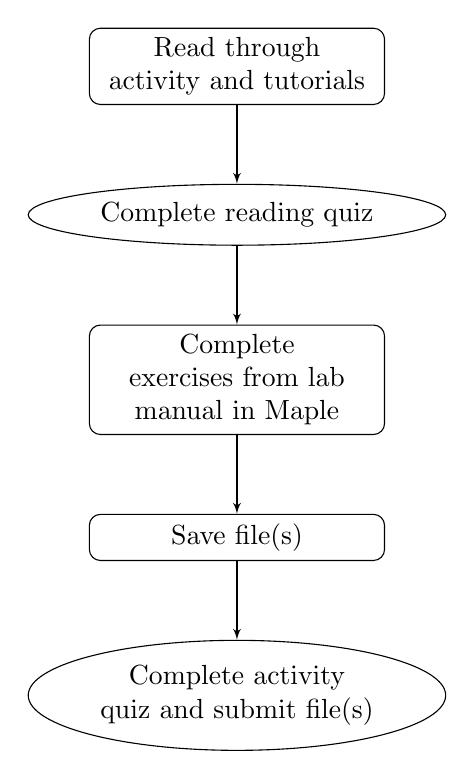
\begin{tikzpicture}[auto]
    	% place nodes
    	\node [rectangle, draw, text centered, rounded corners, text width=10em] (read) {Read through activity and tutorials};
    	\node [ellipse, draw, text centered, rounded corners, text width=10em, below=1cm of read] (readquiz) {Complete reading quiz};
    	\node [rectangle, draw, text centered, rounded corners, text width=10em, below=1cm of readquiz] (activity) {Complete exercises from lab manual in Maple};
    	\node [rectangle, draw, text centered, rounded corners, text width=10em, below=1cm of activity] (save) {Save file(s)};
    	\node [ellipse, draw, text centered, rounded corners, text width=10em, below=1cm of save] (quiz) {Complete activity quiz and submit file(s)};
    	% Draw edges
    	\path [draw, -latex'] (read) -- (readquiz);
    	\path [draw, -latex'] (readquiz) -- (activity);
    	\path [draw, -latex'] (activity) -- (save);
    	\path [draw, -latex'] (save) -- (quiz);
    \end{tikzpicture}
    \caption{Workflow for each weekly activity.}
\end{marginfigure}

\subsection*{Prior to lab} 
Before lab, read through the activity as well as the recommended tutorials from the back of the book. Once you have read through the instructions and tutorials, you will need to complete the \textbf{reading quiz} for the activity.

\marginnote[1cm]{Some lab computers take a couple minutes to log into. Always give yourself a few extra minutes at the start of lab to log in.}

\subsection*{Start of lab}
After logging into the school computer, you should begin by opening up the latest version of Maple as well your lab section's Moodle page. You are expected to have this lab manual with you during lab and you should complete all exercises in order. It is a great idea to have a pen or pencil handy to take notes in your manual while you complete the exercises. Your lab instructor will be available to assist you with the activity, though you will find that many of your questions can be answered by looking through the tutorial sections at the back of this book.

\marginnote[-.4cm]{Always bring your lab manual along to your lab. Take lots of notes in it!}

\subsection*{End of lab}
Once you have completed the exercises, make sure to save your work! You are now ready to complete the \textbf{activity quiz}. The questions in this quiz should be relatively quick to answer once you have completed the exercises from the activity. Often, you can simply copy and paste the output from Maple into the blanks on the quiz. You will be required to \textbf{submit your Maple work} in addition to the quiz.

\marginnote{The questions on your Moodle quiz relate to the exercises in this book. Make sure to finish your exercises prior to the quiz.}

\subsection*{Final lab}
During your final lab, you will be expected to complete an open-book \textbf{lab test}. The test will be based upon the activities that you have completed throughout the semester. You are permitted to have this manual during the test.

% \clearpage

% \section*{Evaluation}
% Your lab grade is determined as follows:
% %\begin{tcolorbox}
% \begin{table}[h]
% \centering
% \begin{tabular}{ll}
% Reading Quizzes                 & 15\%\\
% Activity Submission and Quizzes	& 60\%\\
% Lab Test		            	& 25\%\\
% \hline
% Total			            	& 100\%
% \end{tabular}
% \end{table}
% %\end{tcolorbox}
% \par Your lab grade is transferred to instructor of your lecture session at the end of the semester and accounts for 10\% of your overall Math 112/122 grade.

\section*{Lab Test}
During your lab test, you will be permitted the following materials:
\vspace*{-1ex}
\begin{multicols}{2}
\begin{itemize}
\item This lab manual
\item Handwritten notes
\item Maple help
\columnbreak
\item Previously completed activities
\vfill\null
\end{itemize}
\end{multicols}
\noindent The following are not allowed:
\vspace*{-1ex}
\begin{multicols}{2}
\begin{itemize}
\item Discussion with other students
\item Cell phones
\item Other electronic devices
\item Email
\item Internet (other than Moodle for file submission)
\vfill\null
\end{itemize}
\end{multicols}
You will be allowed to ask for clarification on questions, but will not be allowed to ask for assistance in completing a question or resolving an error in your work.
\par
You will be expected to submit your work electronically and any duplicate submissions will receive a grade of zero. It is important to save your work frequently in case your computer encounters a serious error.
\marginnote[-1cm]{Don't forget to save your file in your \textbf{network folder}. This folder is accessible from any computer. Saving your files is explained in detail in the next chapter.}

\chapter{Introduction to Maple}
\label{chp:introduction}

\section*{The Maple Computer Algebra System}
In lab, you will be using the latest version of Maple, which is a symbolic and numeric computing environment. Maple provides an interface for analyzing, exploring, visualizing, and solving mathematical problems. The interface also allows you to maintain an easy-to-follow document so that you can retrace your thought process. If you plan to pursue any branch of mathematics or field that relies on mathematics, having basic knowledge of a computer algebra system is a very useful tool.

\section*{How to Use This Manual}
This book is divided into two main parts:
\begin{itemize}
\item[\textbf{Part \ref{pt:Activities}}] consists of activities for you to complete. These activities are divided into two chapters: Math 112 and Math 122. Each activity focuses on one topic from that course and contains a list of exercises for you to complete with Maple. Some of these exercises may give very explicit instructions for typing a command into Maple, while others may require you to use your own intuition and understanding of the capabilities of Maple.
\item[\textbf{Part \ref{pt:Tutorials}}] consists of several chapters that provide examples of the usage of common commands in Maple. Many of these examples are designed to be minimalistic in order to show you their basic usage. Each of these examples was completed within Maple and should be reproducible on your own computer.
\end{itemize}
At the beginning of each activity, a list of the most relevant tutorials is given. It is expected that you read through those tutorials as you complete the exercises of that activity. Many activities build upon previously learned commands, so it is a good idea to thoroughly read through all of the relevant tutorials as you progress through lab.

\section*{Accessing Maple and Saving Your Work}
Maple is installed on all lab computers as well as on computers in the library. However, personal copies of Maple are not available through Okanagan College at this time.

\subsection*{Opening Maple on School Computers}

\begin{marginfigure}
\centering

\includegraphics[width=1cm]{introduction/figures/horizonvmware.png}
\caption{You may need to open the VMware Horizon Client first using this desktop icon.}
\end{marginfigure}

On some Windows computers, the most recent version of Maple may be installed directly. In this case, you can simply hit the Start Menu key on your keyboard (in the lower left corner) and begin typing the word "Maple". If Maple is installed directly, then Windows Search will automatically find the version installed and display a link to the application. Alternatively, you should be able to find Maple by browsing the list of installed programs on the Start Menu.

On other computers, you may need to log into a virtual machine to access Maple remotely. On these machines, you will typically find a link to VMware Horizon Client on the desktop. You will need to open this client and log into the remote machine using the same information as you previously used to log into the computer. Once the remote machine loads, you should find Maple in the Start Menu as described above.

\begin{marginfigure}[-5cm]
\centering
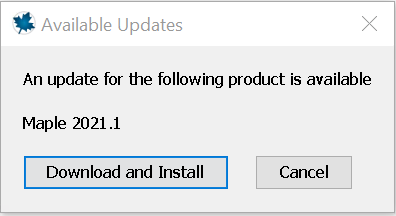
\includegraphics[width=5cm]{introduction/figures/mapleupdate.png}
\caption{After opening Maple, you may be prompted to update the version. You can click Cancel on this dialog box.}
\end{marginfigure}

\subsection*{Organizing Files in your Network Folder}

\begin{marginfigure}
\centering

\includegraphics[width=1.5cm]{introduction/figures/networkfoldershortcut.png}

\includegraphics[width=1cm]{introduction/figures/fileexplorer.png}
\caption{The shortcut for your network folder is on the desktop. You can also open File Explorer with the shortcut on the taskbar.}
\end{marginfigure}

You are given your own personal folder on the network in which to save your files. This folder is accessible from any computer on campus and from VMware Horizon, so you should save all of your work in this folder. You can find this folder by using the desktop shortcut or by opening up File Explorer and clicking on This PC.

\begin{figure}
\centering
\adjincludegraphics[width=0.9\textwidth,trim={0 {0.3\height} 0 0},clip]{introduction/figures/thispc}
\caption{Your network folder should appear under This PC when using File Explorer.}
\end{figure}

\clearpage

It is best to create a new subfolder in your network folder for your lab. This folder could be called something like "Math 112 Labs" so that it is easy to find and organize all of your saved Maple files. When you wish to save your file in Maple, now you can navigate to this folder and save your file with the name of the activity.

\begin{figure}
\centering
\adjincludegraphics[width=0.9\textwidth,trim={0 {0.3\height} 0 0},clip]{introduction/figures/fileorganization}
\caption{Make sure to create a folder for your lab inside your network folder. Save all of your files here using obvious names so that they are easy to find again later.}
\end{figure}

The files that Maple saves are only readable through Maple. However, you can find the Export As tool under the File menu. From there, you can change the file type to PDF and save your document. PDF files can be read by other programs, but cannot be edited by Maple.

\begin{figure}
\centering
\adjincludegraphics[width=0.3\textwidth,trim={0 {0.3\height} {0.2\width} 0},clip]{introduction/figures/exportas}
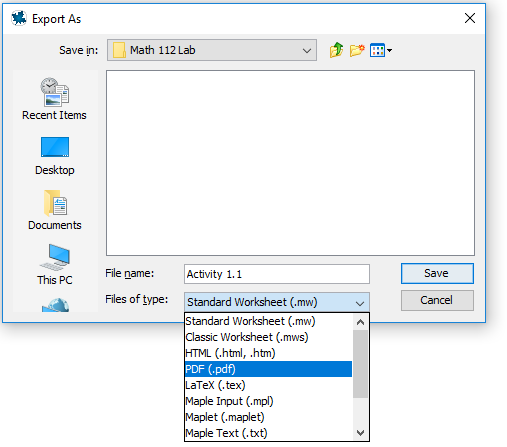
\includegraphics[width=0.6\textwidth]{introduction/figures/exportpdf.png}
\caption{You can export your Maple worksheet as a PDF file type, which can be opened on most devices without Maple. However, Maple cannot edit PDF files.}
\end{figure}

The files that you have saved on your network folder on campus can be accessed from home through a browser by using the following address:

\begin{center}
    \url{https://myfiles.okanagan.bc.ca/}
\end{center}

%----------------------------------------------------------------------------------------------
%----------------------------------------------------------------------------------------------
\mainmatter

\part{Activities}
\label{pt:Activities}

\chapter{Activities for Math 112}
\label{Calc1Activities}

The following list serves as a suggestion for which activities are considered core versus optional:
\begin{table}[h]
\begin{tabular}{lll}
\ref{sec:creating_a_maple_worksheet}
\nameref{sec:creating_a_maple_worksheet}					& pg. \pageref{sec:creating_a_maple_worksheet}					& Core\\
\ref{sec:basics}
\nameref{sec:basics}										& pg. \pageref{sec:basics}										& Core\\
\ref{sec:assignment_operator_and_creating_functions}
\nameref{sec:assignment_operator_and_creating_functions}	& pg. \pageref{sec:assignment_operator_and_creating_functions}	& Core\\
\ref{sec:transformations_of_graphs}
\nameref{sec:transformations_of_graphs}						& pg. \pageref{sec:transformations_of_graphs}					& Optional\\
\ref{sec:solving_equations_in_maple}
\nameref{sec:solving_equations_in_maple}					& pg. \pageref{sec:solving_equations_in_maple}					& Core\\
\ref{sec:limits}
\nameref{sec:limits}										& pg. \pageref{sec:limits}										& Core\\
\ref{sec:limits_and_asymptotes}
\nameref{sec:limits_and_asymptotes}							& pg. \pageref{sec:limits_and_asymptotes}						& Optional\\
\ref{sec:applied_limit_problem}
\nameref{sec:applied_limit_problem}							& pg. \pageref{sec:applied_limit_problem}						& Optional\\
\ref{sec:derivative_of_a_function}
\nameref{sec:derivative_of_a_function}						& pg. \pageref{sec:derivative_of_a_function}					& Core\\
\ref{sec:tangent_lines}
\nameref{sec:tangent_lines}									& pg. \pageref{sec:tangent_lines}								& Optional\\
\ref{sec:building_a_roller_coaster}
\nameref{sec:building_a_roller_coaster}						& pg. \pageref{sec:building_a_roller_coaster}					& Optional\\
\ref{sec:implicit_functions}
\nameref{sec:implicit_functions}							& pg. \pageref{sec:implicit_functions}							& Core\\
\ref{sec:orthogonal_curves}
\nameref{sec:orthogonal_curves}								& pg. \pageref{sec:orthogonal_curves}							& Optional\\
\ref{sec:newtons_method}
\nameref{sec:newtons_method}								& pg. \pageref{sec:newtons_method}								& Core\\
\ref{sec:shape_of_a_can}
\nameref{sec:shape_of_a_can}								& pg. \pageref{sec:shape_of_a_can}								& Optional\\
% \ref{sec:rainbows}
% \nameref{sec:rainbows}										& pg. \pageref{sec:rainbows}									& Optional\\
\ref{sec:sweet_16}
\nameref{sec:sweet_16}										& pg. \pageref{sec:sweet_16}									& Optional
\end{tabular}
\end{table}
		
\section{Creating a Maple Worksheet}
\label{sec:creating_a_maple_worksheet}	

\subsection*{Recommended Tutorials:}
\begin{itemize}[noitemsep]
	\item \nameref{chp:maple_environment}, pg. \pageref{chp:maple_environment}
	\item \nameref{chp:basics_of_maple_syntax}, pg. \pageref{chp:basics_of_maple_syntax}
		\item \nameref{chp:basic_operations}, pg. \pageref{chp:basic_operations}
\end{itemize}

\subsection*{Introduction:}

This activity will give you practice with:
\begin{itemize}
\item setting up a new worksheet in Maple for future activities.
\item switching between paragraphs for text and execution groups for Maple input.
\item evaluating expressions in exact and decimal form.
\end{itemize}

\subsection*{Exercises:}

\begin{enumerate}
	\item Open up Maple on your lab computer. If you are asked whether you would like to update Maple, you can select No. You should now have a blank worksheet for the following exercises.
	\marginnote[0.7cm]{The output of these commands is not useful on its own. However, you have now told Maple to clear its memory and that you would like numerical answers to be displayed with up to $15$ digit accuracy.} 
		
	\item On the first line of your worksheet you should be in Maple input, which is indicated by the \texttt{>} at the start of the line. Type in your first two commands, hitting Enter to run each command:
		\par \texttt{> restart;} \index{restart}
		\par \texttt{> Digits := 15;}\index{Digits}
		
	\item Create a new paragraph for text using 
\includegraphics[width=0.04\textwidth]{tutorials/figures/new_text.png} and type in the following information:
	\marginnote{Ctrl+Shift+J and Ctrl+Shift+K are useful shortcuts for creating paragraphs after or before the current line.}
	\begin{enumerate}
		\item Your first and last name.
		\item Your student number.
		\item The name of your instructor.
		\item The title of the activity.
	\end{enumerate}
	
	\item Open up the palettes menu on the top left-hand side of Maple by clicking the small black triangle that points to the right. You may wish to use the Expression palette for the next few exercises.
	
    \item \label{ex-maple-input} Create a new execution group by using the 
\includegraphics[width=0.05\textwidth]{tutorials/figures/new_input.PNG} button and evaluate $5 + 2(7-4)$.
    \marginnote[-0.7cm]{Ctrl+J and Ctrl+K are useful shortcuts for creating execution groups after or before the current line.}
    
    \item Create a new execution group and evaluate $\left(\dfrac{5^2 - 9}{9-5}\right)^2$.
    \marginnote[-0.4cm]{You can create a fraction by encasing the numerator, $5^2-9$, in a set of parentheses before dividing. Alternatively, you can highlight $5^2-9$ and hit the \texttt{/} key to make a fraction.}
    \clearpage
    \marginnote[0.2cm]{To input a square root, use the \texttt{sqrt()} command.} \index{mathematical functions!square root}
    \item Create a new execution group and evaluate $\sqrt{\dfrac{3+6^2}{4^2-3}}$.
    \marginnote[0.2cm]{Whenever possible, Maple will produce output in exact form. However, using decimals in a Maple input will produce output in decimal form (called a floating point decimal).}
    \item  Create a new execution group and evaluate $\sqrt{\dfrac{3.0+6.0^2}{4.0^2-3.0}}$. \label{ex-sqrt-digits}
    
    \item For each of the following, create a new execution group and evaluate the expression. \label{ex-builtin-functions}
    \begin{enumerate}
        	\marginnote[0.2cm]{The mathematical constant $\pi = 3.14\hdots$\index{Pi} must be typed into Maple as capitalized \texttt{Pi}. Do not type \texttt{pi}, as this is simply the Greek letter $\pi$.}
    	\item $\cos\!\left(\frac{\pi}{6}\right)$
    	\item $\arcsin\!\left(\frac{\sqrt{3}}{2}\right)$
    	\item $\exp(2)$
    	\marginnote{The \texttt{exp(x)}\index{mathematical functions!exponential} function is the exponential function, ${\rm e}^x$. If you type ${\rm e}^x$ using the 'e' key on the keyboard, Maple will not recognize it as the exponential function.}
    	\item $\ln\!\left(5^{\sfrac{1}{2}}\right)$
    \end{enumerate}
    
    \item \label{ex-evalf} On each of the four Maple inputs you created in exercise \ref{ex-builtin-functions}, add a semicolon at the end of the line, followed by the command \texttt{evalf(\%)}. For example:
    \par \texttt{> cos(Pi/6); evalf(\%);}
        \marginnote[-0.7cm]{The semicolon \texttt{;} separates commands if you want to run multiple commands on the same Maple input.}
    
    
    \item If you have accidentally created any additional paragraphs or execution groups that you wish to delete, then delete them now by clicking on that line and pressing Ctrl+Del on the keyboard.
    	\marginnote[0.1cm]{Use the 
\includegraphics[width=0.1\textwidth]{tutorials/figures/new_section.PNG} buttons to create or remove sections. Alternatively, the shortcuts Ctrl+. and Ctrl+, can be used to enclose execution groups of paragraphs in a section or remove any section enclosing an input.} 
    	
    \item Organize your work by using a new section for each of exercises \ref{ex-maple-input}-\ref{ex-evalf}. Be sure to clearly label each question by creating a section title immediately to the right of the arrow at the top of the section.
    \marginnote[0.1cm]{You can highlight several execution groups or paragraphs with the mouse before combining them into one section.}
    \item (Optional) Go back to the top of your worksheet and change the second line to:
    \par \texttt{> Digits := 50;}
    \par Now run each Maple input again by hitting Enter on each line or by pressing the 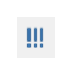
\includegraphics[width=0.05\textwidth]{activities/math112/figures/execute_button.eps} button. What changed?
    \marginnote[-1cm]{You do not need to have your cursor at the end of the line to run the command. Hitting Enter with your cursor anywhere on the Maple input will run the command.}
    
    \marginnote[0.2cm]{Pressing the 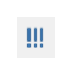
\includegraphics[width=0.05\textwidth]{activities/math112/figures/execute_button.eps}\index{execute entire worksheet} button executes every command in the entire worksheet.}
\end{enumerate}
\section{The Basics}
\label{sec:basics}

\subsection*{Recommended Tutorials:}
\begin{itemize}[noitemsep]
	\item \nameref{chp:basic_operations}, pg. \pageref{chp:basic_operations}
	\item \nameref{chp:plotting_functions}, pg. \pageref{chp:plotting_functions}
\end{itemize}

\subsection*{Introduction:}

In this activity, you will learn basic usage of some of the most common Maple commands:
\par
\begin{minipage}[t]{0.5\textwidth}
\begin{itemize}
\item \texttt{expand()}\index{expand}
\item \texttt{factor()}\index{factor}
\end{itemize}
\end{minipage}
\begin{minipage}[t]{0.5\textwidth}
\begin{itemize}
\item \texttt{simplify()}\index{simplify}
\item \texttt{plot()}\index{plot}
\end{itemize}
\end{minipage}

\subsection*{Exercises:}
\begin{enumerate}
    \item Expand the polynomial $(2x-y)^6$.
    \item Factor the polynomial $16x^4-160x^3y+600x^2y^2-1000xy^3+625y^4$.
    \marginnote{When two or more variables appear next to each other, be sure to include a \texttt{*} or space between them, so that Maple knows that they are multiplied together.}
    \item Simplify the expression $\dfrac{x^3-1}{x-1}$.
    \item Now we would like Maple perform all three commands together.
    \marginnote{It is a good practice when using the \% \index{ditto operator} shortcut to run the commands simultaneously on the same Maple input.}
    \begin{enumerate}
    	\item Have Maple expand the rational expression $\dfrac{(x-y)^2+(x+y)^2}{x^3-y^3}$.
    	\item Add a semicolon to the end of the line, followed by \texttt{simplify(\%)}.
    	\item Add another semicolon to the end of the line, followed by \texttt{factor(\%)}.
    	\item Hit Enter to run all three commands together.
    \end{enumerate}
    \marginnote{You can add a line break between commands without running them with Shift+Enter.}
    You should see three outputs now: expanding, simplifying, and factoring.
    \item (Optional) Consider polynomials of the form $x^p-1$, where $p$ is a prime number. Try factoring each of the following:
    \begin{enumerate}
		\begin{minipage}[t]{0.5\textwidth}
    	\item $x^2 - 1$
    	\item $x^3 - 1$
    	\item $x^5 - 1$
		\end{minipage}
		\begin{minipage}[t]{0.5\textwidth}
    	\item $x^7 - 1$
    	\item $x^{19} - 1$
		\end{minipage}
    \end{enumerate} 	
    Can you notice a pattern and show that these polynomials follow a particular form when factored? To explain your solution, use the 
\includegraphics[width=.04\textwidth]{tutorials/figures/new_text.PNG} button to create a new paragraph after the current line.
    \marginnote[-0.5cm]{Ctrl+Shift+J can also be used to create a paragraph after the current line.}
    \newpage
    \item Plot\index{plot} the following two functions using separate \texttt{plot()} commands and note the difference in domain:
    \begin{enumerate}
    	\item $x^{\sfrac{1}{3}}$
    	\item $\texttt{surd}(x,3)$\index{mathematical functions!nth root@$n$\textsuperscript{th} root}
    	\marginnote[-1cm]{The \texttt{surd(x,3)} function is equivalent to $\sqrt[3]{x}$. Similarly, \texttt{surd(x,5)} is equivalent to $\sqrt[5]{x}$, etc.}
    \end{enumerate}
    \item On a new Maple input, create a plot\index{plot} of the following list of functions
    \begin{center}
    \texttt{[ x\^{}2, x\^{}3, sqrt(x), surd(x,3), abs(x) ]}\index{plot!multiple functions}
    \end{center}
    and include the following options (separated by commas).
    \marginnote{Square brackets in Maple are used to create a comma-separated list of items in the specified order.}
    \begin{itemize}
    \item \texttt{x = -5..10} \hfill\textit{(This specifies the $x$-axis)}\index{plot!axes intervals}
    \item \texttt{y = -5..10} \hfill\textit{(This specifies the $y$-axis)}
    \item \texttt{colour = [red,blue,green,purple,orange]} \index{plot!colours}
    \end{itemize}
    \marginnote[-0.5cm]{An example of plotting multiple functions at once can be found on page \pageref{sec:plotting_multiple_functions}.}\index{plot!multiple functions}
\end{enumerate}
\section{The Assignment Operator and Creating Functions}
\label{sec:assignment_operator_and_creating_functions}		

\subsection*{Recommended Tutorials:}
\begin{itemize}[noitemsep]
	\item \nameref{chp:plotting_functions}, pg. \pageref{chp:plotting_functions}
	\item \nameref{chp:assignment_operator}, pg. \pageref{chp:assignment_operator}
\end{itemize}

\subsection*{Introduction:}

In this activity, you will be using the assignment operator \texttt{:=}, which allows you assign Maple output to a name of your choice. This is especially useful for assigning expressions and functions on one Maple input, before manipulating those expressions later on in your worksheet.

\subsection*{Exercises:}
\begin{enumerate}
    \item Assign the expression $ \dfrac{\sin(x)+3}{\cos(x)+1}$ to \texttt{expr} and then use the \texttt{subs()} command to substitute $x=3$ into \texttt{expr}. Evaluate this as a decimal with $15$ digits.
    \item Assign the expression $x^2+2^x$ to \texttt{expr2} and substitute $y = $~\texttt{expr2} into the expression $y^2+3y$. 
    \marginnote[0.2cm]{Instead of using the \texttt{subs} command multiple times, it is often a better practice to define a function and use function notation instead.}
    \item  Assign the expression $2x^2-4x+7$ to \texttt{poly} and then substitute $x=5+h$ into \texttt{poly} and simplify.
    
    \item Consider the function $f(x) = (1-x^2) {\rm e}^{-\sfrac{x^2}{2}}$. \marginnote{The exponential function, ${\rm e}^x$, in Maple is denoted as  \texttt{exp(x)}.}
    \index{mathematical functions!exponential}
    \begin{enumerate}
    	\item Assign the function to $f(x)$. 	
    	\marginnote[0.2cm]{When assigning the function to $f(x)$, use the $:=$ operator.}\index{assignment operator}
   		\item This function $f(x)$ is known as the \textit{Mexican Hat Function}. Can you see why? Plot the graph of $f(x)$.
    \end{enumerate}
    \item Maple, by default, does not know the function
    \marginnote{Often, this function is denoted as ${\rm sinc}_\pi(x)$ and ${\rm sinc}(x) = \frac{\sin (x)}{x}$.}
   	\[ sinc(x) = \dfrac{\sin(\pi x)}{\pi x}, \]
   	which is important in engineering. 
   	\marginnote[-0.3cm]{Be sure to include a multiplication symbol or space between $\pi$ and $x$.}\index{Pi}
   	\marginnote[0.1cm]{The mathematical constant $\pi = 3.14\hdots$ must be typed into Maple as \texttt{Pi}.}\index{Pi}
   	\begin{enumerate}
	   	\item Assign this function to $sinc(x)$.   	\marginnote[0.2cm]{When assigning the function to $sinc(x)$, use the $:=$ operator.}\index{assignment operator}
	   	\item Evaluate $sinc(3)$, $sinc\left(\frac{1}{2}\right)$, and $sinc(0.25)$.
	   	\item Plot the graph of $sinc(x)$.
   	\end{enumerate}
\end{enumerate}
\section{Transformations of Graphs}
\label{sec:transformations_of_graphs}

\subsection*{Recommended Tutorials:}
\begin{itemize}[noitemsep]
	\item \nameref{chp:plotting_functions}, pg. \pageref{chp:plotting_functions}
	\item \nameref{chp:assignment_operator}, pg. \pageref{chp:assignment_operator}
\end{itemize}

\subsection*{Introduction:}

In this activity, you will plot multiple functions at once to investigate basic transformations of functions.

\subsection*{Exercises:}
\begin{enumerate}
    \item Plot the graphs of $\sin (x)$ and $\cos (x)$ on the same set of axes. Use \textit{red} for $\sin (x)$ and \textit{blue} for $\cos (x)$.  
    \marginnote{If you do not specify the $x$-axis interval, Maple will default to increments of $\pi/8$ from $-2\pi$ to $2\pi$.}
    \begin{enumerate}
    	\item By what amount do you need to shift the graph of $\sin (x)$ \textit{to the left} (negative $x$ direction) so that it coincides with the graph of $\cos (x)$? Answer the question in sentence form by using the 
\includegraphics[width=0.04\textwidth]{tutorials/figures/new_text.PNG} button to create a new paragraph after the current line.
        \marginnote[-0.5cm]{An example of plotting multiple functions at once can be found on page \pageref{sec:plotting_multiple_functions}.}
    	\item By what amount do you need to shift the graph of $\sin (x)$ \textit{to the right} (positive $x$ direction) so that it coincides with the graph of $\cos (x)$? Write your answer in sentence form using a new paragraph.
    \end{enumerate}
    
    \item The graphs of ${\rm e}^x$ and $\ln(x)$ should appear to be reflected over the line $y=x$. Plot all three graphs on the same axes using \texttt{linestyle=[solid,solid,dash}].\index{plot!line style}
    \marginnote[-1.3cm]{The \texttt{exp(x)} function is the exponential function, ${\rm e}^x$.}
    \marginnote[-0.3cm]{When plotting functions of the form $y=f(x)$ using the \texttt{plot()} command, we omit the $y=$.}
    \marginnote[0.3cm]{When assigning the function to $f(x)$, use the $:=$ operator.}
        \index{assignment operator}
	\item Assign the function $f(x) = \sqrt{-x^2 + 4x + 21}$. \\Plot each of the following functions on the same set of axes:
	\[y = f(x), \, y = f(2x), \, y = 3f(x), \, y = f(-x), \, y = -f(x).\]
	Make sure that the graph is displayed with constrained scaling ($1:1$). Describe each transformation. Write your answer using a new paragraph.
	\marginnote[-1.2cm]{An example of plotting transformations of a function can be found on page \pageref{subsec:plotting_transformations}.}
	\marginnote[0cm]{It is always a good practice to specify the colours of multiple graphs in order to tell them apart. A list of plot colours can be found by typing \texttt{?colours} on a new Maple input.}\index{plot!colours}
	
    \item Plot each of the following graphs separately:
    \marginnote[0.5cm]{The absolute value function $|\cdot|$ in Maple is denoted as \texttt{abs( )}.}
\index{mathematical functions!absolute value}
    \begin{enumerate}
    	\item $y = \sin(x)$
    	\item $y = \sin(|x|)$
    	\item $y = |\sin(x)|$
    \end{enumerate}
    Create a new paragraph to describe the transformations of \\$y = \sin(x)$ in parts (b) and (c).
\end{enumerate}
\section{Solving Equations in Maple}
\label{sec:solving_equations_in_maple}		

\subsection*{Recommended Tutorials:}
\begin{itemize}[noitemsep]
	\item \nameref{chp:equation_solvers}, pg. \pageref{chp:equation_solvers}
\end{itemize}

\subsection*{Introduction:}

In this activity, students will be asked to assign expressions and then evaluate and manipulate them.

\subsection*{Exercises:}
\begin{enumerate} 
    \item Suppose we want to find the $x$-intercepts of the function \[ f(x) = x^5+x^4-4x^3-3x^2+3x+1.\] 
    \begin{enumerate}
        	\item Assign the function to $f(x)$.  \marginnote[-0.1cm]{When assigning the function to $f(x)$, use the $:=$ operator.}
        	\index{assignment operator}
    	\item Plot $f(x)$. Choose an interval for $x$ that shows all $x$-intercepts. How many do you see?
    	\item Factor $f(x)$. Does $f(x)$ factor? 
    	\item Solve $f(x)=0$ using both the \texttt{solve()} and \texttt{fsolve()} commands.
    	\marginnote[-1.2cm]{With \texttt{fsolve()}, you can also specify an interval for solutions if you wish to only find a particular solution. An example of this can be found on page \pageref{eg:fsolve_interval}.}
    	\index{solving equations!solve}	\index{solving equations!fsolve}
    \end{enumerate}
    \item Solve the quadratic equation $x^2+4x+6=0$ three ways:
    
    \begin{enumerate}
    	\item Using the quadratic formula by hand. \marginnote[-0.5cm]{Given a quadratic equation of the form $ax^2+bx+c=0$, the quadratic formula is
\[x=\dfrac{-b\pm \sqrt{b^2-4ac}}{2a}.\]}
    	\item Using \texttt{solve()}, followed by evaluating the result as a decimal.
    	\item Using \texttt{fsolve()}.
    \end{enumerate}
    Compare your results from (b) and (c).
    \marginnote[-0.2cm]{In Maple, $\sqrt{-1}$ is denoted as $I$.}\index{imaginary}

    \item Consider the curves $y=x^2$ and $y=\frac{3}{x}$.
        \marginnote[0.6cm]{An example that shows how to find the intersection point of two functions is given on page \pageref{subsec:functionintersection}.}
    \begin{enumerate}
    \item Find the point $(x,y)$ where the two curves intersect. Try using both the \texttt{solve()} and \texttt{fsolve()} commands.
    
    \item Plot the two curves on the same set of axes to verify that your intersection point from part (a) is correct.
    \marginnote[-0.4cm]{When plotting equations of the form $y=f(x)$ using the \texttt{plot()} command, we never include the $y=$.}
    \marginnote[0.2cm]{When multiple curves are plotted on the same set of axes, it is a good practice to specify the colour of each one, so that you can tell them apart.}
	\end{enumerate}     
    
\end{enumerate}
\section{Limits}
\label{sec:limits}

\subsection*{Recommended Tutorials:}
\begin{itemize}[noitemsep]
	\item \nameref{chp:limits}, pg. \pageref{chp:limits}
\end{itemize}

\subsection*{Introduction:}

In this activity, students will use the \texttt{limit()}\index{limit} command to find various limits.

\subsection*{Exercises:}
\begin{enumerate}
    \item Calculate the limit $\displaystyle\lim_{x \to 1} \dfrac{\ln(x^4+1)-1}{x-2}$.
\marginnote[-0.5cm]{There is a shortcut for limits on the palettes toolbar under Calculus.\begin{center}
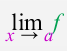
\includegraphics[scale=0.5]{tutorials/figures/palettelimit.png}
\end{center}}
    \item Plot the function 
    \[f(x)=\dfrac{|x|}{x}\] 
    over an appropriate range, and then use the \texttt{limit()}\index{limit} command to calculate the left-hand limit, the right-hand limit, and the two-sided limit as $x$ tends to zero.
    \marginnote[-1.8cm]{In Maple, the absolute value function $|\cdot|$ is denoted as \texttt{abs( )}.} \index{plot!discontinuities}
    \marginnote[-0.9cm]{Some versions of Maple may not properly display graphs of certain functions that contain discontinuities. In this case, include \texttt{discont=true} as a parameter in the \texttt{plot( )} command.}
    \item Consider the function $g(x)=\dfrac{x^2+x}{\sqrt{x^3+x^2}}.$
    \marginnote[0.1cm]{Use \texttt{sqrt()} to input a square root in Maple.}
			\begin{enumerate}
				\item Use the \texttt{plot()} command between $x=-2$ and $x=2$ to estimate the left-hand-limit, the right-hand limit, and the two-sided limit as $x$ tends to zero.
				\marginnote[0.1cm]{You need to find the limit as $x$ approaches zero, not as it approaches $-2$ or $2$.}
				\item Use the \texttt{limit()} command to verify your results from part (a).

			\end{enumerate}

    \item Estimate the value of 
    \[\displaystyle\lim_{t\to 0} \dfrac{\sin(t)}{\sin(\pi t)}\] 
    by using Maple's \texttt{plot()} command, and then check your answer with Maple's \texttt{limit()} command.
    	\marginnote[-1cm]{Do not forget to use \texttt{Pi} for $\pi$ and include multiplication between $\pi$ and $t$. You will also need to use $t$ instead of $x$ in your \texttt{plot()} command!}
		\item Calculate $\displaystyle\lim_{x \to \infty} \sqrt{x+1}-x$.\index{limit!at infinity}
    \marginnote[-0.2cm]{To denote $\infty$ in Maple, you need to type the word \texttt{infinity}.}
    \item Use the Limit Methods Tutor to explore the steps to calculate 
    \[\displaystyle\lim_{x \to -\infty} \sqrt{x^2+x+1}+x.\]\index{limit!at infinity}
    \marginnote[-1cm]{The Limit Methods Tutor is described on page \pageref{sec:limitmethodstutor}.}
    \index{limit!tutor}
\end{enumerate}
\section{Limits and Asymptotes}	
\label{sec:limits_and_asymptotes}	

\subsection*{Recommended Tutorials:}
\begin{itemize}[noitemsep]
	\item \nameref{chp:limits}, pg. \pageref{chp:limits}
\end{itemize}

\subsection*{Introduction:}

It is incorrect to assume that a vertical asymptote is always found whenever the denominator of a rational function is equal to zero. Instead, we say that $f(x)$ has a vertical asymptote at $x=a$ whenever
\[ \dlim{x}{a^+} f(x) = \infty \]
or
\[ \dlim{x}{a^-} f(x) = \infty. \]
In either case, the equation of the vertical asymptote\index{limit!one-sided}\index{asymptote!vertical} is $x=a$.

Similarly, a horizontal asymptote \index{limit!at infinity}\index{asymptote!horizontal}of $f(x)$ is also defined in terms of limits. A function $f(x)$ has a horizontal asymptote $y = L$ if
\[ \dlim{x}{\infty} f(x) = L \]
or
\marginnote{While a function may have many vertical asymptotes, it cannot have more than two horizontal asymptotes.}
\[ \dlim{x}{-\infty} f(x) = L. \]
In this case, the equation of the horizontal asymptote is $y=L$.

You will need to use both of these definitions while answering the following exercises.

\subsection*{Exercises:}
\begin{enumerate} \index{plot!discontinuities}
    \marginnote[-0.54cm]{Some versions of Maple may not properly display graphs of functions that contain vertical asymptotes. In this case, include \texttt{discont=true} as a parameter in the \texttt{plot( )} command. An example of finding vertical asymptotes is given on page \pageref{subsec:vertical_asymptotes}.}
    \item Plot the function $f(x)=\dfrac{x-1}{x^2-x-2}$ and estimate its vertical asymptotes. Use Maple to prove that your guesses are, in fact, the vertical asymptotes by taking the one-sided limits at those values. Insert a new paragraph and state the equations of the vertical asymptotes.
\marginnote[-0.3cm]{The 
\includegraphics[width=0.04\textwidth]{tutorials/figures/new_text.PNG} button or Ctrl+Shift+J can be used to create a paragraph after the current line.}       

    \item Consider the function $g(x)=\dfrac{x+2}{x^2-x-6}$.
    \begin{enumerate}
    \item Use Maple to factor the denominator of $g(x)$.
    \marginnote[-0.5cm]{If you use Maple's \texttt{denom()}\index{mathematical functions!denominator} command and type \texttt{denom($g(x)$)}, you will get the denominator of $g(x)$.}
    \item By factoring the denominator of $g(x)$, you might suspect that the vertical asymptotes are $x=-2$ and $x=3$. Plot $g(x)$ and show why this may or may not be the case.
    \end{enumerate}
    

    \item Consider the function $h(t)=\dfrac{\sin(t)}{t}$.\index{mathematical functions!sine}
    \begin{enumerate}
        \item Plot\index{plot} a graph of $h(t)$.
        \item Use Maple's \texttt{limit()}\index{limit} command to find the horizontal asymptote(s) of $h(t)$. 
        \marginnote{An example of finding horizontal asymptotes\index{asymptote!horizontal} is provided on page \pageref{subsec:horizontal_asymptotes}.}
        \item Insert a new paragraph and state the equation(s) of the horizontal asymptote(s)\index{asymptote!horizontal}.
      \end{enumerate}


\item Consider the function  $Q(x)=\dfrac{\sqrt{2x^2+1}}{3x+5}$.
\marginnote{The \texttt{sqrt()}\index{mathematical functions!square root} command is used to input a square root.}  
    \begin{enumerate}
        \item Plot a graph of $Q(x)$. Be sure to specify appropriate intervals for the $x$-axis and $y$-axis.
        % \marginnote[-0.6cm]{Does $Q(x)$ have any vertical asymptotes? If so, make sure to use \texttt{discont=true} as a plot option.}
        \item Use Maple's \texttt{limit()} command to find the horizontal asymptote(s) of $Q(x)$. 
        \item Insert a new paragraph and state the equation(s) of the horizontal asymptote(s).
        \marginnote[-0.6cm]{Maple provides a useful \texttt{Asymptotes()}\index{asymptote!asymptote command} command for finding the asymptotes of a function. Try typing \texttt{?Asymptotes} to learn more.}
\end{enumerate}     

\end{enumerate} 
\section{A Shrinking Circle Problem}
\label{sec:applied_limit_problem}

\subsection*{Recommended Tutorials:}
\begin{itemize}[noitemsep]
	\item \nameref{chp:equation_solvers}, pg. \pageref{chp:equation_solvers}
	\item \nameref{chp:limits}, pg. \pageref{chp:limits}
\end{itemize}

\subsection*{Introduction:}

Limits may seem trivial when you first learn them, but they are fundamental building blocks in calculus. They are used to explain terms like ``infinitesimally small'' and ``infinitely large''. It may be interesting to know that they can also be used in applied problems. This activity will explore a geometry problem and will solve it using limits, instead of an elementary geometric approach.

Figure \ref{fig:applied_limit} below shows two circles:
\begin{itemize}
	\item $C_1$, centred at the point $(1,0)$ with radius $1$ and equation \[(x-1)^2+y^2=1.\]
	\item $C_2$, centred at the origin with radius $r$ and equation \[x^2+y^2=r^2.\]
\end{itemize}

\begin{figure}[h]
\centering
\label{fig:applied_limit}
\caption{What happens to the point $R$ as the radius of the thicker circle $C_2$ shrinks?}
\pgfplotsset{compat=1.5.1}
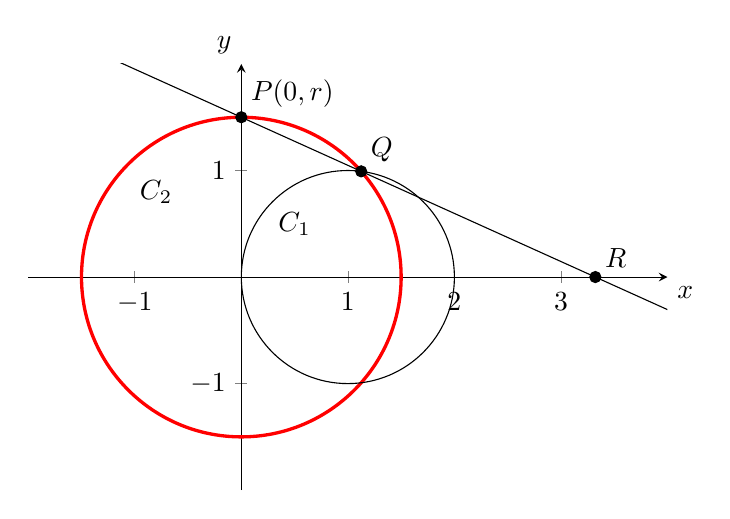
\begin{tikzpicture}[shift={(0,0)}]
	\begin{axis}[
	width=0.8\linewidth,
	axis lines=middle,
	xlabel={$x$},
	ylabel={$y$},
	xlabel style={below right},
	ylabel style={above left},
	xmin=-2, xmax=4, xtick={-1,0,1,2,3},
	ymin=-2, ymax=2, ytick={-1,0,1},
    axis equal image
	]
	\addplot[domain=-2:4] {1.500000000-.4514162296*x};
	\addplot[mark=*] coordinates {(0,1.5)} node [above right] {$P (0,r)$};
	\addplot[mark=*] coordinates {(1.125000000,0.9921567417)} node [above right] {$Q$};
	\addplot[mark=*] coordinates {(3.322875656,0)} node [above right] {$R$};
	\draw(axis cs:0,0) [very thick, red] circle[radius=1.5];
	\draw(axis cs:-0.8,0.8) node {$C_2$};
	\draw(axis cs:1,0) circle[radius=1];
	\draw(axis cs:0.5,0.5) node {$C_1$};
	\end{axis}
\end{tikzpicture}
\end{figure}

If we define $P$ as the point $(0,r)$ at the top of the circle $C_2$, and $Q$ as the upper point of intersection of the two circles, then we can construct the line $PQ$ and see that it crosses the $x$-axis. Let $R$ be the $x$-intercept of the line $PQ$.

\marginnote{Note that neither $P$ nor $Q$ is fixed as the radius of $C_2$ shrinks.}
Now, begin to shrink the radius of circle $C_2$; that is, let $r\rightarrow 0^{+}$. What happens to the point $R$ as $C_2$ shrinks?

\subsection*{Exercises:}

\begin{enumerate}
	\item Assign names to the equations of both circles, such as \texttt{C1} and \texttt{C2}.
    \item Find the point of intersection of $C_1$ and $C_2$ in quadrant I. This is the point $Q$. The coordinates of $Q$ should be expressions of $r$.
    \marginnote[-1cm]{You can find the point of intersection with a single \texttt{solve()} command, but you may need to include the optional parameter \texttt{explicit=true} to avoid the \textit{RootOf()} output.}\index{solving equations!removing \texttt{RootOf()}}
	\item We now have two points on the line, $P$ and $Q$, so we can construct the equation of this line. For parts (a) and (b), let $P = (0,r)$ be $(x_1,y_1)$ and let $Q$ (the point you found in exercise 2) be $(x_2,y_2)$.
	\begin{enumerate}
	\item Find the slope of the line $PQ$ using the slope equation \[ m = \frac{y_2 - y_1}{x_2 - x_1}. \]\index{lines!slope}
	\item Define the equation of the line $PQ$ using the slope from part (a) and the point-slope equation of a line	\[ y - y_0 = m (x - x_0). \]\index{lines!point-slope form}
	\end{enumerate}
	\marginnote{Remember that $R$ is the $x$-intercept of the line $PQ$, so its $y$-coordinate is $0$. The $x$-coordinate can be found using the \texttt{subs()}\index{subs}  and \texttt{solve()} \index{solving equations!solve} commands.}
	\item Using the equation of the line you just found, find the coordinates of $R$. 
	\item Now what happens as $r \to 0^+$?\index{limit}
	\marginnote{Use the \texttt{limit()} command as $r$ approaches $0$ from the right.}
\end{enumerate}

%\subsection*{Notes:}
%\begin{itemize}
  %  \item   Use 15 decimal places to find your answers, when applicable.

%\end{itemize}
\section{The Derivative of a Function}
\label{sec:derivative_of_a_function}

\subsection*{Recommended Tutorials:}
\begin{itemize}[noitemsep]
	\item \nameref{chp:assignment_operator}, pg. \pageref{chp:assignment_operator}
	\item \nameref{chp:equation_solvers}, pg. \pageref{chp:equation_solvers}
	\item \nameref{chp:derivative}, pg. \pageref{chp:derivative}
\end{itemize}

\subsection*{Introduction:}

In this activity, we will investigate the derivative of a function and use Maple's powerful computational skills to simplify the process of finding a derivative.

\subsection*{Exercises:}

\begin{enumerate}
    \item  Consider the function $f(x) = \sqrt{9 - x}$.
    \marginnote[-0.2cm]{To input a square root, use the \texttt{sqrt()} command.}  \index{mathematical functions!square root}
    \marginnote[0.2cm]{When assigning the function to $f(x)$, use the $:=$ operator.}
    \begin{enumerate}
    	\item Define this function in Maple.
    	\item Find the derivative\index{derivative}, $f'(x)$, using the \texttt{limit()}\index{limit} command and the limit definition of the derivative.
    	\marginnote[-0.3cm]{Don't forget! \[f'(x) = \dlim{h}{0}\dfrac{f(x+h)-f(x)}{h}\]}\index{limit!definition of a derivative}
    	\item Find the derivative, $f'(x)$, using the \texttt{diff()}\index{derivative!diff} command.
    	\item Find the derivative, $f'(x)$, using \texttt{'}\index{derivative!prime notation} notation.
%    	\item Define the equation of the tangent lines at $x=0$ and $x=5$.
%    	\item Plot $f(x)$ and the two tangent lines on the same axes.
    \end{enumerate}
    \item A toy rocket is fired straight upward, and its height (in metres) is given by: $h(t) = t + 10 - \sqrt{2t^2 + 100}$, with $0 \leq t \leq 20$, where $t$ is the time in seconds.
    \marginnote[-0.8cm]{If you decide to define a height function, be sure that the variable in your function name matches the variable in your function.}
    \begin{enumerate}
    	\item Plot\index{plot} a graph of height as a function of time.
    	\item Find a formula for velocity in terms of $t$.
    	\marginnote[-0.3cm]{Recall that the derivative of position with respect to time is velocity.}
    	\item At what time is the velocity $0$ m/s?
    	\item What is the maximum height that the rocket attains?
    	\marginnote[-0.5cm]{When the velocity of the rocket is $0$ m/s, the rocket has reached its maximum height.}
    	\marginnote[0.5cm]{An example of finding minimum and maximum values on a closed interval can be found on page \pageref{subsec:closed_interval_method}.}
    \end{enumerate}
    \item Molten lava can fill a chamber in the earth's crust before it builds up enough pressure to erupt. Let the pressure be modeled by $P(t) = 0.47 t^2 {\rm e}^{0.0035 t}$, where $t$ is the time in months.
    \marginnote[1cm]{Recall that \texttt{exp()} \index{mathematical functions!exponential} is used to denote the exponential function in Maple.}
    \begin{enumerate}
    	\item What is the rate of change of pressure with respect to time?
    	\item Suppose that an eruption is highly likely to occur if pressure increases at a rate greater than $20$. Is an eruption likely when $t=30$ months? Use a new paragraph to state your answer.
    \end{enumerate}
    \newpage
	\item Consider the function $g(x)=\sin(2\pi^2 x)$.\index{mathematical functions!sine}
		\marginnote[-0.1cm]{To type the mathematical constant $\pi = 3.14\hdots$\index{Pi}, be sure to use \texttt{Pi}. }
		\marginnote[0.1cm]{Don't forget to include multiplication between $\pi^2$ and $x$.}
	\begin{enumerate}
	\item Use Maple to find the first derivative, the second derivative, the third derivative, and the fourth derivative of $g(x)$. You should notice a pattern, so use a new paragraph to describe it.
	\marginnote[-0.1cm]{The $n$\textsuperscript{th} derivative\index{derivative!diff!higher derivatives}\index{derivative!prime notation!higher derivatives} of the function can be computed by using the \texttt{diff()} command or \texttt{'} notation. See page \pageref{chp:derivative} for more information. You can also make use of the Calculus palette:
	\begin{center} 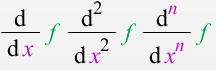
\includegraphics[scale=0.6]{tutorials/figures/palettediff.png}
 \end{center} }
	\item Use your answer from part (a) to predict what the $77$\textsuperscript{th} derivative of $g(x)$ is, and then verify that your prediction is correct by computing this derivative using Maple.
	\item (Optional) Use the information in Tutorial \ref{chp:conditional_statements_and_loops} on page \pageref{chp:conditional_statements_and_loops} to write a loop\index{loops} that will output the first $100$ derivatives of $g(x)$.
	\end{enumerate}
\end{enumerate}

%\subsection*{Notes:}
%\begin{itemize}
%    \item  
%\end{itemize}
\section{Tangent Lines}
\label{sec:tangent_lines}	

\subsection*{Recommended Tutorials:}
\begin{itemize}[noitemsep]
	\item \nameref{chp:assignment_operator}, pg. \pageref{chp:assignment_operator}
	\item \nameref{chp:equation_solvers}, pg. \pageref{chp:equation_solvers}
	\item \nameref{chp:derivative}, pg. \pageref{chp:derivative}
\end{itemize}

\subsection*{Introduction:}

In this activity, students will find tangent lines to various functions, and then will display the tangent lines and function on the same graph.\\

\noindent To find the tangent line to a function $f(x)$ at $x = a$, two pieces of information are needed:
\begin{itemize}
\item The point, $(a, f(a))$.
\item The slope of the tangent line, $f'(a)$.
\end{itemize}
\marginnote{A detailed example of finding and plotting tangent lines is described on page \pageref{subsec:equation_of_tangent_line}.}
Plugging these two pieces of information into the point-slope form of a line gives the following equation.
\begin{align}
y - y_0 &= m_{tan} \cdot (x-x_0) \nonumber\\ 
y - f(a) &= f'(a) \cdot (x-a) \nonumber\\
y &= f'(a) \cdot (x-a) + f(a) \label{eq:tanline}
\end{align}\index{lines!tangent line}\index{lines!slope of a tangent line}
We will use equation \eqref{eq:tanline} for the following exercises.

\subsection*{Exercises:}
\begin{enumerate}
	\item  Consider the function $f(x) = \sqrt{9 - x}$.
    \begin{enumerate} \marginnote[-0.5cm]{Be sure to choose different names for each tangent line. If you assign a new expression to an old name, the new expression will overwrite what was previously assigned.}
    	\item Define the equations of the tangent lines at $x=0$ and $x=5$.
    	
    	\item Plot $f(x)$ and the two tangent lines on the same axes.\index{plot!multiple functions}
    	\marginnote[0.1cm]{Since you are plotting more than one
tangent line on the same axes, it is a good idea to specify plot colours.}
    \end{enumerate}
    \item Consider the function $g(x)=x{\rm e}^{x}$.\index{mathematical functions!exponential}
    \marginnote[0.3cm]{In Maple, \texttt{exp(x)} is used to denote the exponential function, ${\rm e}^x$.}\index{mathematical functions!exponential}
		\begin{enumerate}
			\item Define the equations of the tangent lines at $x=1$ and $x=-1$.
			\item Plot $g(x)$ and the two tangent lines on the same axes.
		\end{enumerate}
	\item Consider the function $h(x)=x^3-x^2-9x+9$. 
	\begin{enumerate}
		\item Find the $x$-values where the function has tangent lines with slope equal to $1$. 
		\item Find the $x$-values where the function has horizontal tangent lines\index{lines!horizontal tangent line}.
		\marginnote[-0.5cm]{To solve part (b), you need to remember what the slope of a horizontal tangent line is.}
%		\item Find the equation of the tangent line at $x=2$, then plot the function and the tangent line on the same set of axes.
	\end{enumerate}
\end{enumerate}
%\subsection*{Notes:}
%\begin{itemize}
%    \item   
%\end{itemize}
\section{Building a Roller Coaster}
\label{sec:building_a_roller_coaster}

\subsection*{Recommended Tutorials:}
\begin{itemize}[noitemsep]
	\item \nameref{chp:assignment_operator}, pg. \pageref{chp:assignment_operator}
	\item \nameref{chp:equation_solvers}, pg. \pageref{chp:equation_solvers}
	\item \nameref{chp:derivative}, pg. \pageref{chp:derivative}
\end{itemize}

\subsection*{Introduction:}
You are in charge of designing the first hill of a new roller coaster. For an initial design, you connect a straight stretch of track for the lift hill followed by two parabolas, as shown in Figure \ref{fig:rollercoaster}.

\begin{figure*}[h]
\label{fig:rollercoaster}
\hspace{-3cm}
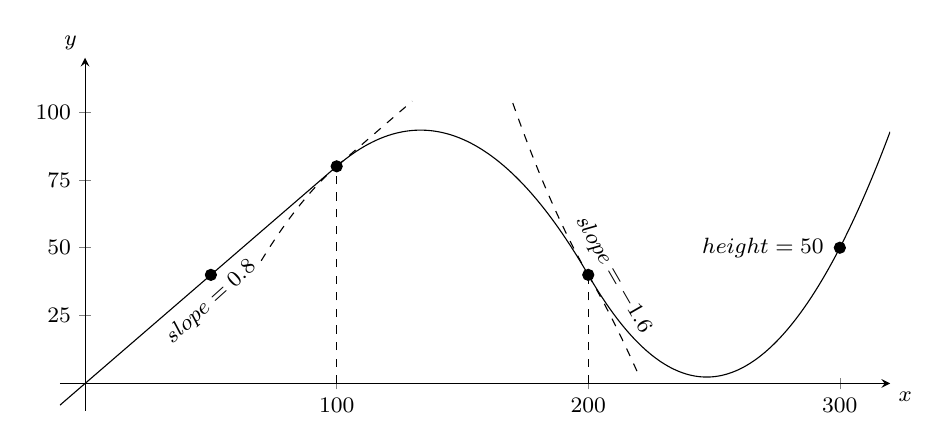
\begin{tikzpicture}
\footnotesize
\begin{axis}[
	width=\textwidth,
	height=0.5\textwidth,
	axis lines=middle,
	xlabel={$x$},
	ylabel={$y$},
	xlabel style={below right},
	ylabel style={above left},
	xmin=-10, xmax=320, xtick={0,100,200,300},
	ymin=-10, ymax=120, ytick={0,25,50,75,100}
]
	\addplot [domain=-10:100, samples=100] {0.8*x};
	\addplot [domain=100:130, samples=100, dashed] {0.8*x};
	\addplot [domain= 70:100, samples=100, dashed] {(-0.012)*x^2+3.2*x-120};
	\addplot [domain=100:200, samples=100] {(-0.012)*x^2+3.2*x-120};
	\addplot [domain=200:220, samples=100, dashed] {(-0.012)*x^2+3.2*x-120};
	\addplot [domain=170:200, samples=100, dashed] {0.017*x^2+((-1)*8.4)*x+1040};
	\addplot [domain=200:320, samples=100] {0.017*x^2+((-1)*8.4)*x+1040};
	\addplot[mark=*] coordinates {(50,40)};
	\draw [dashed] (axis cs:100,0) -- (axis cs:100,80);
	\addplot[mark=*] coordinates {(100,80)};
	\draw(axis cs:50,30) node [rotate=42] {$slope = 0.8$};
	\addplot[mark=*] coordinates {(200,40)};
	\draw [dashed] (axis cs:200,0) -- (axis cs:200,40);
	\draw(axis cs:210,40) node [rotate=-60] {$slope = -1.6$};
	\addplot[mark=*] coordinates {(300,50)} node [left] {$height=50~$};
\end{axis}
\end{tikzpicture}
\caption{A simple design for the initial hill of a roller coaster.}
\end{figure*}
% OLD PSTRICKS CODE
%	\psset{xunit=1.2pt,yunit=1.2pt}
%	\begin{pspicture}(-10,120)(320,-10)
%	\psaxes[ticksize=-2pt 2pt,Dx=50,Dy=20]{->}(0,0)(-10,-10)(320,120)
%	\psplot[algebraic=true,VarStep=true,showpoints=false,plotpoints=100,linewidth=1.0pt]{-10}{100}{0.8*x}
%	\psplot[algebraic=true,VarStep=true,showpoints=false,plotpoints=100,linewidth=1.0pt,linestyle=dashed]{100}{130}{0.8*x}
%	\psplot[algebraic=true,VarStep=true,showpoints=false,plotpoints=100,linewidth=1.0pt,linestyle=dashed]{70}{100}{(-0.012)*x^2+3.2*x-120}
%	\psplot[algebraic=true,VarStep=true,showpoints=false,plotpoints=100,linewidth=1.0pt]{100}{200}{(-0.012)*x^2+3.2*x-120}
%	\psplot[algebraic=true,VarStep=true,showpoints=false,plotpoints=100,linewidth=1.0pt,linestyle=dashed]{200}{220}{(-0.012)*x^2+3.2*x-120}
%	\psplot[algebraic=true,VarStep=true,showpoints=false,plotpoints=100,linewidth=1.0pt,linestyle=dashed]{170}{200}{0.017*x^2+((-1)*8.4)*x+1040}
%	\psplot[algebraic=true,VarStep=true,showpoints=false,plotpoints=100,linewidth=1.0pt]{200}{320}{0.017*x^2+((-1)*8.4)*x+1040}
%	\psline(100,0)(100,80)
%	\psline(200,0)(200,40)
%	\psline(300,0)(300,50)
%	\end{pspicture}
\noindent
The following criteria must be met to build the roller coaster:
\begin{itemize}
	\item The lift hill will have a slope of $0.8$.
	\item The straight section of the lift hill will cover a horizontal distance of $100$ ft.
	\item The slope of the first descent will reach a maximum magnitude of $1.6$ after another $100$ ft.
	\item The next hill will reach a height of $50$ ft after another $100$ ft.
	\item The track must be smooth (i.e. there cannot be any sudden changes in the slope of the track).
\end{itemize}

\clearpage

\subsection*{Exercises:}
The goal of the following exercises is to develop a piecewise function that satisfies all of the above criteria.

\begin{enumerate}
	\item Let $L(x)$ be the function for the lift hill, which is a linear function passing through the origin. 
	\begin{enumerate}
		\marginnote[0.5cm]{The lift hill function can easily expressed in $y=mx+b$ form.}\index{lines!slope-intercept form}
		\item Using the given criteria, assign the function $L(x)$ in Maple for the lift hill.
		\item Determine the $x$- and $y$-coordinates at which the lift hill connects to the first parabola, $f(x)$.
	\end{enumerate}
	
	\item Let $f(x)$ be the function for the first parabola, opening downward. We will define this function in a few steps.
	\begin{enumerate}
		\item Assign the function $f(x)=ax^2+bx+c$ as a general quadratic function. We will solve for the coefficients using the above criteria over the next two steps.
		\marginnote[0.5cm]{Be sure to include multiplication between variables.}
		\item We can solve for $a$, $b$, and $c$, by using three equations. Write an equation in function notation for each of the following conditions.
			\marginnote{Each of these equations can be written in the form of \[f(\alpha)=\beta\] or \[f'(\alpha)=\beta.\]}
			\begin{itemize}
			\item $f$ must pass through the point from exercise 1(b).
			\item The derivative of $f$ at $x=100$ is $0.8$, so that the track is smooth (differentiable) where it connects to the lift hill.
			\item The derivative of $f$ at $x=200$ is $-1.6$, according to the given criteria.
			\end{itemize}
	\item Use a \texttt{solve()}\index{solving equations!solve}	 or \texttt{fsolve()}\index{solving equations!fsolve}	 command and function notation to solve the system of equations for $a$, $b$, and $c$.
		\item Reassign the function $f(x)$ using the values you have just calculated.
		\item Determine the $x$- and $y$-coordinates at which the $f(x)$ connects to the next parabola (when $x=200$).
	\end{enumerate}
	
	\item Let $g(x)$ be the function for the second parabola, opening upward. We will define this function in a few steps.
	\begin{enumerate}
		\marginnote[0.5cm]{Be sure to include multiplication between variables.}
		\item Assign a function $g(x)=px^2+qx+r$ as a general quadratic function. We will solve for the coefficients using the above criteria over the next two steps.
		\item We can solve for $p$, $q$, and $r$, by using three equations. Write an equation in function notation for each of the following conditions.
			\begin{itemize}
			\item $g$ must pass through the point from exercise 2(e).
			\item The derivative of $g$ at $x=200$ is $-1.6$ so that the track is smooth (differentiable) where it connects to $f(x)$.
			\marginnote[-0.5cm]{Each of these equations can be written in the form of \[g(\alpha)=\beta\] or \[g'(\alpha)=\beta.\]}
			\item The height of $g$ at $x=300$ is $50$, according to the given criteria.
			\end{itemize}
		\item Use a \texttt{solve()} or \texttt{fsolve()} command and function notation to solve the system of equations for $p$, $q$, and $r$.
		\item Reassign the function $g(x)$ using the values you have just calculated.
	\end{enumerate}
	\marginnote[1cm]{The \texttt{piecewise()} command can be found on page \pageref{chp:assignment_operator}.}
	\item Use the \texttt{piecewise()} command to define a piecewise function\index{mathematical functions!piecewise} called \textit{coaster(x)} that consists of the three pieces:\\
		$coaster(x) = \left\lbrace
			\begin{array}{ll}
			L(x)	&	0 \leq x < 100 \\
			f(x)	&	100 \leq x < 200 \\
			g(x)	&	200 \leq x \leq 300
			\end{array}
		\right.$
	\item Plot the piecewise function, \textit{coaster(x)}.
\end{enumerate}
\section{Implicit Functions}
\label{sec:implicit_functions}	

\subsection*{Recommended Tutorials:}
\begin{itemize}[noitemsep]
	\item \nameref{chp:equation_solvers}, pg. \pageref{chp:equation_solvers}
	\item \nameref{chp:implicit_functions}, pg. \pageref{chp:implicit_functions}
\end{itemize}

\subsection*{Introduction:}

In this activity, we will learn how to plot implicit functions, as well as compute their derivatives.

\marginnote[-5cm]{There are a few important things to remember about the \texttt{implicitplot()} command during this activity:
	\begin{itemize}
	\item The \texttt{plots} package needs to be loaded using the \texttt{with()} command. 
	\item Some versions of Maple may not produce a smooth plot. In this case, include either \texttt{numpoints=30000} or \texttt{grid=[250,250]} as a parameter.
	\item The optional \texttt{scaling=constrained} parameter can be included to enforce $1:1$ scaling. Alternatively, the optional scaling can be performed by clicking on the graph and then clicking on the $1:1$ button in the plot toolbar at the top of the page.
	\item If you are plotting multiple graphs on the same set of axes, it is a good idea to specify plot colours.
	\end{itemize}
}

\vspace{2cm}

\subsection*{Exercises:}
\begin{enumerate}
    \marginnote{A similar example is described on page \pageref{subsec:implicittanline}.}
    \item  Consider the circle centred at the origin with radius $5$. 
    \marginnote[1cm]{The equation of a circle that is centred at the point $(a,b)$ and has radius $r$ is
    \[(x-a)^2+(y-b)^2=r^2.\]}\label{Mathematical function!Circle}
    \begin{enumerate}
    	\item Define the equation for this circle and plot it. Ensure that the circle appears smooth.
    	\item Find the $y$-coordinates of the points when $x=2$.
    	\item Compute the derivative, $\frac{dy}{dx}$\index{derivative}, of the circle.
    	\item Find the slopes of the lines tangent to the circle at $x=2$.
    	\marginnote[.3cm]{Recall that the tangent line\index{lines!tangent line} equation to the curve at the point $(x_0,y_0)$ is \[y=m\cdot(x-x_0)+y_0,\] where $m=\frac{dy}{dx}\Bigr|_{(x_0,y_0)}$.}
    	\item Define the equations of the tangent lines to the curve at both points when $x=2$. Be sure to assign different names for each tangent line and include $y=$ in the equations of the lines so that the \texttt{implicitplot()}\index{implicit functions!implicitplot} command can plot them. Expand each of these tangent line equations so that they are written in the form $y=mx+b$.
    	\item Plot the circle and the two tangent lines.
    \end{enumerate}
    
    \marginnote[.3cm]{Do not forget to include multiplication between variables.}
    \item Consider the Folium of Descartes: $x^3 + y^3 = 6xy.$

    \begin{enumerate}
    	\item Define this curve and plot it. Ensure the curve appears smooth.
    	\item Compute the derivative, $\frac{dy}{dx}$.
    	\marginnote{In exercise (c), try using the \texttt{solve()} command first, then change it to \texttt{fsolve()} if necessary.}
    	\item Find the equations of each of the tangent lines at the points where $x=1$. Plot the Folium of Descartes and the tangent lines on the same graph.
    	\marginnote{To solve part (d), you need to remember that the slope is zero when the tangent line is horizontal.\index{lines!horizontal tangent line} The equation $\frac{dy}{dx} = 0$ and the equation of the curve itself form a system of equations that can be solved by Maple to give the $x$ and $y$ value of each point. An example of solving a system of equations can be found on page \pageref{sec:solvingsystemeqs}.}
    	\item Find any points on the Folium of Descartes where the tangent lines are horizontal.
    \end{enumerate}
\end{enumerate}
\section{Orthogonal Curves}
\label{sec:orthogonal_curves}

\subsection*{Recommended Tutorials:}
\begin{itemize}[noitemsep]
	\item \nameref{chp:equation_solvers}, pg. \pageref{chp:equation_solvers}
	\item \nameref{chp:implicit_functions}, pg. \pageref{chp:implicit_functions}
\end{itemize}

\subsection*{Introduction:}

Orthogonal curves are curves that are perpendicular whenever they intersect. Perpendicular lines\index{lines!perpendicular lines} are an elementary example of this. We know that if $m_1$ and $m_2$ are the slopes of two perpendicular lines, then $m_1 m_2 = -1$. Similarly, two curves are orthogonal if their derivatives multiply to $-1$ whenever they intersect.

\marginnote[-6cm]{There are a few important things to remember about the \texttt{implicitplot()} command during this activity:\index{implicit functions!implicitplot}
	\begin{itemize}
	\item The \texttt{plots} package needs to be loaded using the \texttt{with()} command. 
	\item Some versions of Maple may not produce a smooth plot. In this case, include either \texttt{numpoints=30000} or \texttt{grid=[250,250]} as a parameter.
	\item The optional \texttt{scaling=constrained}\index{implicit functions!implicitplot!scaling} parameter can be included to enforce $1:1$ scaling. Alternatively, the optional scaling can be performed by clicking on the graph and then clicking on the $1:1$ button in the plot toolbar at the top of the page.
	\item If you are plotting multiple graphs on the same set of axes, it is a good idea to specify plot colours.\index{implicit functions!implicitplot!multiple plots}\index{implicit functions!implicitplot}
	\end{itemize}
}
\vspace{1cm}
\subsection*{Exercises:}

\begin{enumerate}
	\marginnote{Do not forget to include multiplication between $x$ and $y$.}
    \item Consider the curves $y^2 - x^2 = 3$ and $xy = 2$.
    \begin{enumerate}
    	\item Plot both of these curves on the same set of axes. Make sure both curves appear smooth.
    	\marginnote[-0.4cm]{In order to find points of intersection, Maple can solve a system of equations in one \texttt{solve()} \index{solving equations!solve} or \texttt{fsolve()}\index{solving equations!fsolve} command for both $x$ and $y$. If you choose to use the \texttt{solve()} command, you may need to include the optional parameter \texttt{explicit=true} to avoid the \textit{RootOf()} output.}
    	\item Find the $x$- and $y$-coordinates of the points of intersection.
    	\item Compute the derivatives of both curves.
    	\marginnote[0.3cm]{A similar example is detailed on page \pageref{subsec:orthocurves}.}
    	\item Are these curves orthogonal at the points of intersection? Confirm this using the fact that $m_1 m_2 = -1$ for perpendicular slopes.
    \end{enumerate}
    \index{solving equations!removing \texttt{RootOf()}}
    \vspace{0.8cm}
    \item Consider the two families of curves given by \[ y = cx^2 \] and \[ x^2 + 2y^2 = k, \] where $c$ and $k > 0$ are arbitrary constants. 
    \marginnote[0.8cm]{Be sure to include $y=$ when using the \texttt{implicitplot()} command to plot the curves for the first family.}
    \begin{enumerate}
    	\item Plot several curves of the first family using 
    	\[ c=-2,-1,0,1,2 \] 
    	\marginnote[0.2cm]{You may wish to make all curves of the same family the same colour.}
    	and several curves of the second family using
    	\[ k=1,4,9 \]
    	on the same axes.
    	\item Find the $x$ and $y$ coordinates of the four intersection points of the two families of curves. The coordinates of the points should be given in terms of $c$ and $k$.
    	\item Compute the derivative of each family of curves. 
    	\marginnote{It is a good idea to use the assignment operator $:=$ to assign each derivative in part (c) to a name. This will allow you to easily reference the derivatives when completing part (d).}
    	\item Show that the two families of curves are orthogonal at each of the four intersection points, regardless of $c$ and $k$.
    \end{enumerate}
\end{enumerate}
\section{Newton's Method}\index{Newton's method}
\label{sec:newtons_method}

\subsection*{Recommended Tutorials:}
\begin{itemize}[noitemsep]
	\item \nameref{chp:derivative}, pg. \pageref{chp:derivative}
	\item \nameref{chp:conditional_statements_and_loops}, pg. \pageref{chp:conditional_statements_and_loops}
\end{itemize}

\subsection*{Introduction:}

Newton's method is an algorithm that can be used to approximate the root of a continuous function. In class, we learned that the linear approximation for $f(x)$ at $x=a$ is given by the function
\marginnote{There are some practical considerations you should be aware of when using Newton's method including: 
\begin{enumerate}
\item how difficult it is to compute the derivative, 
\item poor initial guesses, and 
\item convergence to the wrong root.  
\end{enumerate} 
Any of these will lead Newton's method to be less useful.}
\[ L(x) = f'(a) (x-a) + f(a). \] \index{Newton's method!formula}
Now, suppose we are given a continuous function $f$ with a root $r$ and wish to approximate $r$. One way we could do this is to choose a value $a$ close to $r$, determine the linear approximation $L(x)$ at $x=a$ and find the root of $L(x)$ by setting it to zero:
\[ f'(a) (x-a) + f(a) = 0 .\]
This gives the root of $L(x)$ as
\marginnote{Newton's method will fail for a number of different reasons:
\begin{enumerate}
\item if the starting point leads to a cycle between two or more points, \item if the iteration point is at a critical point, or 
\item if the derivative is discontinuous.
\end{enumerate}   
Be careful of such situations.}
\[ x = a - \frac{f(a)}{f'(a)}. \]
Now, assuming that this value of $x$ is closer to $r$ than our initial value $a$, we could repeat this process again. Therefore, our formula for each new approximation can be simplified to \[x_{new} = x_{old} - \dfrac{f(x_{old})}{f^{\prime}(x_{old})}.\]  By repeated evaluation of this equation, we can continue to find better approximations of $r$.

\begin{figure}[h]
\label{fig:newtonsmethod}
\centering
\caption{Using three iterations of Newton's Method to approximate the root $r$.}
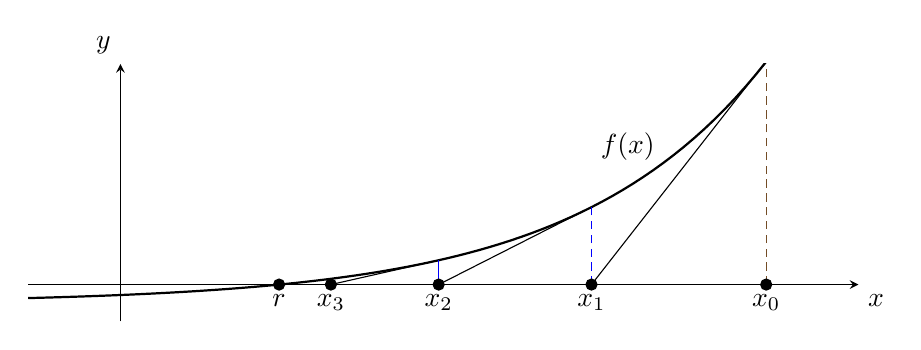
\begin{tikzpicture}
\begin{axis}[
	width=\linewidth,
	height=0.4\linewidth,
	axis lines=middle,
	xlabel={$x$},
	ylabel={$y$},
	xlabel style={below right},
	ylabel style={above left},
	xmin=-10, xmax=80, xtick={0},
	ymin=-20, ymax=120, ytick={0}
]
	\addplot [domain=-10:100, samples=100, thick] {1.05^(x+30)-10};
	\addplot [domain=51.06267696:70, samples=100] {6.415967957*x-327.6164992};
	\addplot [domain=34.49325000:51.06267696, samples=100] {2.546792633*x-87.84715498};
	\addplot [domain=22.80985278:34.49325000, samples=100] {1.134746996*x-25.88341192};
	\addplot[mark=*] coordinates {(17.19363282,0)} node [below] {$r$};
	\addplot[mark=*] coordinates {(70,0)} node [below] {$x_0$};
	\addplot +[mark=none] coordinates {(70,0) (70, 121.5012578)};
	\addplot[mark=*] coordinates {(51.06267696,0)} node [below] {$x_1$};
	\addplot +[mark=none] coordinates {(51.062676960,0) (51.06267696, 42.19889452)};
	\addplot[mark=*] coordinates {(34.49325000,0)} node [below] {$x_2$};
	\addplot +[mark=none] coordinates {(34.49325000,0) (34.49325000, 13.25769989)};
	\addplot[mark=*] coordinates {(22.80985278,0)} node [below] {$x_3$};
	\addplot +[mark=none] coordinates {(22.80985278,0) (22.80985278, 3.15236232)};
	\draw(axis cs:55,75) node {$f(x)$};
\end{axis}
\end{tikzpicture}
\end{figure}
\marginnote[-1.3cm]{Newton's method can be used to approximate the critical points (max or min) of a function.  Since a function $f$ has a maximum or minimum at a point $c$ for which $f^{\prime}(c) = 0$, we can simply change our Newton's method to be \[x_{new} = x_{old} - \dfrac{f^{\prime}(x_{old})}{f^{\prime \prime}(x_{old})}.\]}
In the following exercises, you can make use of the \texttt{NewtonsMethod()} command, provided as part of the \texttt{Student[Calculus1]} package. A useful example can be found in Tutorial \ref{sec:newtonsmethod} on page \pageref{sec:newtonsmethod}. However, it is also beneficial to try more advanced coding methods and implement a ``while" loop if you are interested; information regarding loops is given in Tutorial \ref{chp:conditional_statements_and_loops} on page \pageref{chp:conditional_statements_and_loops}.
\marginnote[-0.5cm]{To load the \texttt{Student[Calculus1]} package, the \texttt{with()} command needs to be used. Make sure you capitalize the appropriate letters in the package name, or else it will not load the necessary commands.}


\subsection*{Exercises:}

\begin{enumerate}
\marginnote[0.2cm]{Be sure to load the \texttt{Student[Calculus1]} package before using the \texttt{NewtonsMethod()} command. The package only needs to be loaded once in your document, not every time you use one of its commands.}\index{Newton's method!NewtonsMethod}
    \item  Use Maple's \texttt{NewtonsMethod()} command to determine the value of the root of the function $f(x) = x^2 - 2$.  Use an initial guess of $2$.  Iterate until you get $10$ decimal places of accuracy.
    \marginnote[0.4cm]{Adding the optional \texttt{iterations} parameter to the \texttt{NewtonsMethod()} command allows you to choose how many iterations are performed. By default, \texttt{NewtonsMethod()} carries out $5$ iterations.}
    
    \marginnote[0.4cm]{The output of Maple's \texttt{NewtonsMethod()} command can be displayed in different ways, depending on whether the \texttt{output} parameter is set equal to \texttt{value}, \texttt{plot}, \texttt{animation}, or \texttt{sequence}. See page \pageref{sec:newtonsmethod} for more information.}
    \item   Apply Newton's method to determine the value of the root of the function $f(x) = x^2 - 2$.  Use an initial guess of $-2$.  Iterate until you get $10$ decimal places of accuracy.
    \item   We cannot use Newton's method to find the root of the function $f(x) = x^2 - 2$ if we use an initial guess of $0$.  Use a graph to help explain why, and discuss your answer by using a new paragraph.
    \item   Suppose you wish to find the value of $\sqrt{7}$ using Newton's method.
	    \begin{enumerate}
	    \item What function would we use if we wanted to apply Newton's method to determine the value of $\sqrt{7}$? State your answer using a new paragraph.
	    \item Evaluate $\sqrt{7}$ to $15$ digits using \texttt{evalf()}. Apply Newton's method to the function from part (a) with an appropriate initial guess for $x$ and verify that the values agree.
	    \end{enumerate}
    \item   Newton's method converges with \textit{quadratic convergence}.  That roughly means that you will get twice as many correct digits for $x_{new}$ as you did for $x_{old}$. Iterate Newton's method for \[g(x) = x^2 - \sin(x) - 0.5\] with an initial guess of $x = 2$.  Find the value of the zero of $g(x)$ to $16$ decimal places.
    
   \item (Optional) Write a "while" loop that allows you to solve exercises 1 and 2.\index{loops}
\end{enumerate}
\section{The Shape of a Can}
\label{sec:shape_of_a_can}	

\subsection*{Recommended Tutorials:}
\begin{itemize}[noitemsep]
	\item \nameref{chp:equation_solvers}, pg. \pageref{chp:equation_solvers}
	\item \nameref{chp:derivative}, pg. \pageref{chp:derivative}
\end{itemize}

\subsection*{Introduction:}
Your goal in this question is to design the most economical shape of a perfectly cylindrical can. 
\begin{figure}[h]
\centering
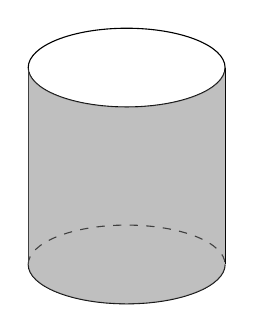
\begin{tikzpicture}
\draw (0,0) ellipse (1.25 and 0.5);
\draw (-1.25,0) -- (-1.25,-2.5);
\draw (-1.25,-2.5) arc (180:360:1.25 and 0.5);
\draw [dashed] (-1.25,-2.5) arc (180:360:1.25 and -0.5);
\draw (1.25,-2.5) -- (1.25,0);  
\fill [gray,opacity=0.5] (-1.25,0) -- (-1.25,-2.5) arc (180:360:1.25 and 0.5) -- (1.25,0) arc (0:180:1.25 and -0.5);
\end{tikzpicture}
\caption{A simple can in the shape of a circular cylinder.}
\end{figure}

First, let us assume the can has to hold a volume of 250 mL (250~cm$^3$). The cylindrical sides as well as the top and bottom circles are cut from sheets of aluminum. The material for the cylindrical sides of the cans is made from rectangles that are bent, so no material is wasted. However, some amount of material is always wasted when trying to cut circles from a sheet of metal. To make the most economical can, your goal is to reduce the \textit{total} amount of material needed, including any wasted metal.
%	\begin{center}
%	\psset{unit=0.8cm}
%    \begin{pspicture}(-1.5,-3)(1.5,1)
%    \psellipse(0,0)(1.5,0.7)
%    \psline(0,0)(1.5,0)
%    \psline(-1.5,0)(-1.5,-2)
%    \psline(1.5,0)(1.5,-2)
%    \psellipse(0,-2)(1.5,0.7)
%    \psframe*[linecolor=white](-1.47,-2)(1.47,-1)
%    \uput[u](0.75,-0.1){$r$}
%    \uput[d](1.8,-.8){$h$}
%    \end{pspicture}
%    \end{center}
%   	\caption{The can}
%   	\label{fig:can}
\begin{figure}[h]
\centering
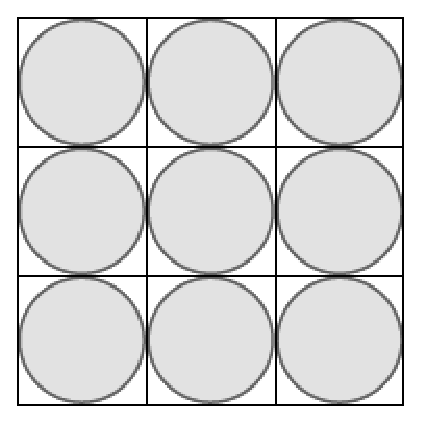
\includegraphics[scale=0.5]{activities/math112/figures/squares.eps}
\label{fig:square}
\caption{Cutting circles in a square pattern.}
\end{figure}
\begin{figure}[h]
\centering
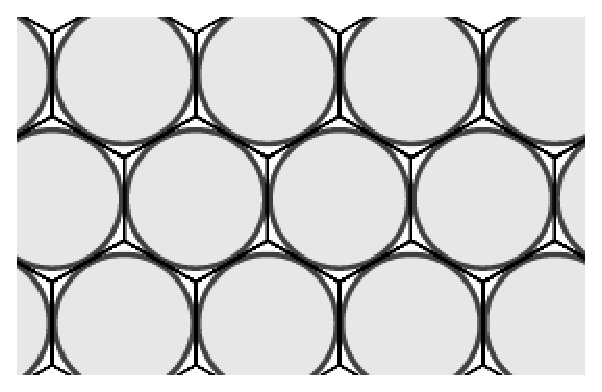
\includegraphics[scale=0.5]{activities/math112/figures/hexagons.eps}
\caption{Cutting circles in a hexagonal pattern.}
\label{fig:hexagon}
\end{figure}
    
If the circles are cut according to Figure \ref{fig:square}, then the total amount of material required for each can is a rectangle and two squares, which wastes a lot of material. If we plan to minimize the amount of material required, we will instead cut out circles according to Figure \ref{fig:hexagon}. The total area of material required for each can then becomes a rectangle and two hexagons.

\subsection*{Exercises:}
We will set up an equation for the total surface area of sheet metal required and then find when it is a minimum.
	\begin{enumerate}
	\marginnote[1cm]{Don't forget that the mathematical constant $\pi$ is represented in Maple as \texttt{Pi}.}\index{Pi}
	\item The side of the can is in the shape of a rectangle that has width $h$ and a length equal to the circumference of the lid. Give an equation for this area in terms of $r$ and $h$.
	\item The two hexagons that are needed for the top and bottom of the can circumscribe a circle of radius $r$. Give an equation for the area of this hexagon in terms of $r$. Figure \ref{hexagoncircle} may be helpful for splitting the hexagon up into six equilateral triangles.
\begin{figure}[h]
\caption{A hexagon circumscribing a circle.}
\centering
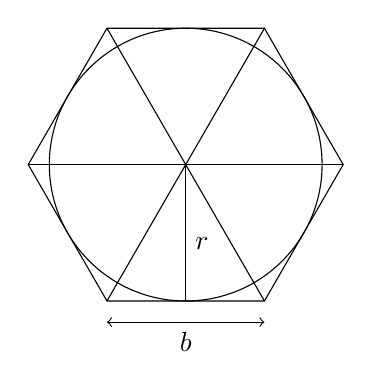
\begin{tikzpicture}
  \draw[] (0,0) circle (1.732050808cm);
  \node[regular polygon, regular polygon sides=6, draw, inner sep=1.2247cm] at (0,0) {};
  \draw (-1,1.732050808) -- (1,-1.732050808);
  \draw (-1,-1.732050808) -- (1,1.732050808);
  \draw (-2,0) -- (2,0);
  \draw (0,-1.732050808) -- (0,-1) node[right] {$r$} -- (0,0);
  \draw [<->] (-1,-2) -- (1,-2);
  \draw (0,-2) node [below] {$b$};
\end{tikzpicture}
%	\psset{unit=1cm}
%	\begin{pspicture}(-2,2)(2,-2)
%    \pspolygon(-1,1.732050808)(1,1.732050808)(2,0)(1,-1.732050808)(-1,-1.732050808)(-2,0)
%    \pscircle(0,0){1.732050808}
%    \psline(0,0)(-1,1.732050808)
%    \psline(0,0)(0,1.732050808)
%    \psline(0,0)(1,1.732050808)
%    \psline(0,0)(1.5,0.866025403)
%    \psline(0,0)(2,0)
%    \psline(0,0)(1.5,-0.866025403)
%    \psline(0,0)(1,-1.732050808)
%    \psline(0,0)(0,-1.732050808)
%    \psline(0,0)(-1,-1.732050808)
%    \psline(0,0)(-1.5,-0.866025403)
%    \psline(0,0)(-2,0)
%    \psline(0,0)(1.5,-0.866025403)
%    \psline(0,0)(-1.5,0.866025403)
%    \uput[60](0,0.866025403){$r$}
%    \end{pspicture}
\label{hexagoncircle}
\end{figure}
	\marginnote[-3cm]{Using trigonometric ratios of $\tfrac{\pi}{3}=60^\circ$ and $\tfrac{\pi}{6}=30^\circ$, it is possible to compute the length of $b$ in terms of $r$.}
	\marginnote[-1cm]{The area of each of the six triangles is $\tfrac{1}{2}br$.}
	\item Give an equation for the total area $A$ required (including waste) as a function of $r$ and $h$. This total area should include two hexagons and the rectangle that is used for the side of the can.
	\marginnote{The volume of a circular cylinder is \[ V=\pi r^2 h.\]}
	\item Given the required total volume $V=250$, use a substitution for $h$ to give the area from exercise 3 in terms of $r$ only. Assign this function as $A(r)$.
	\item Plot a graph of $A(r)$ over the interval $0 \leq r \leq 5$. Limit the vertical range to $-200 \leq A \leq  400$.
	\item Use the second derivative test to find the value of $r$ that minimizes the total area $A(r)$.
	\marginnote[-0.1cm]{For the second derivative test, find Type I critical numbers where $A'(r)=0$. Then show that $A''(r)>0$ for all $r>0$ to indicate that the area is an absolute minimum at this critical number.}
	\item Calculate the height of the can using this radius.
	\clearpage
	\marginnote{It can be shown that the ratio of height to radius of the optimized can is $\dfrac{h}{r} =~\dfrac{4\sqrt{3}}{\pi}$, regardless of volume.}
	\item Show that the ratio of height to radius is $\dfrac{h}{r} = \dfrac{4\sqrt{3}}{\pi} \approx 2.21$.
	\end{enumerate}

% \section{The Calculus of Rainbows}
\label{sec:rainbows}	

\subsection*{Recommended Tutorials:}
\begin{itemize}[noitemsep]
	\item \nameref{chp:equation_solvers}, pg. \pageref{chp:equation_solvers}
	\item \nameref{chp:derivative}, pg. \pageref{chp:derivative}
\end{itemize}

\subsection*{Introduction:}

Rainbows are created when raindrops scatter sunlight. In this project, we use the ideas of Descartes and Newton to explain the shape, location, and colours of rainbows.

\begin{figure}[h]
	\centering
	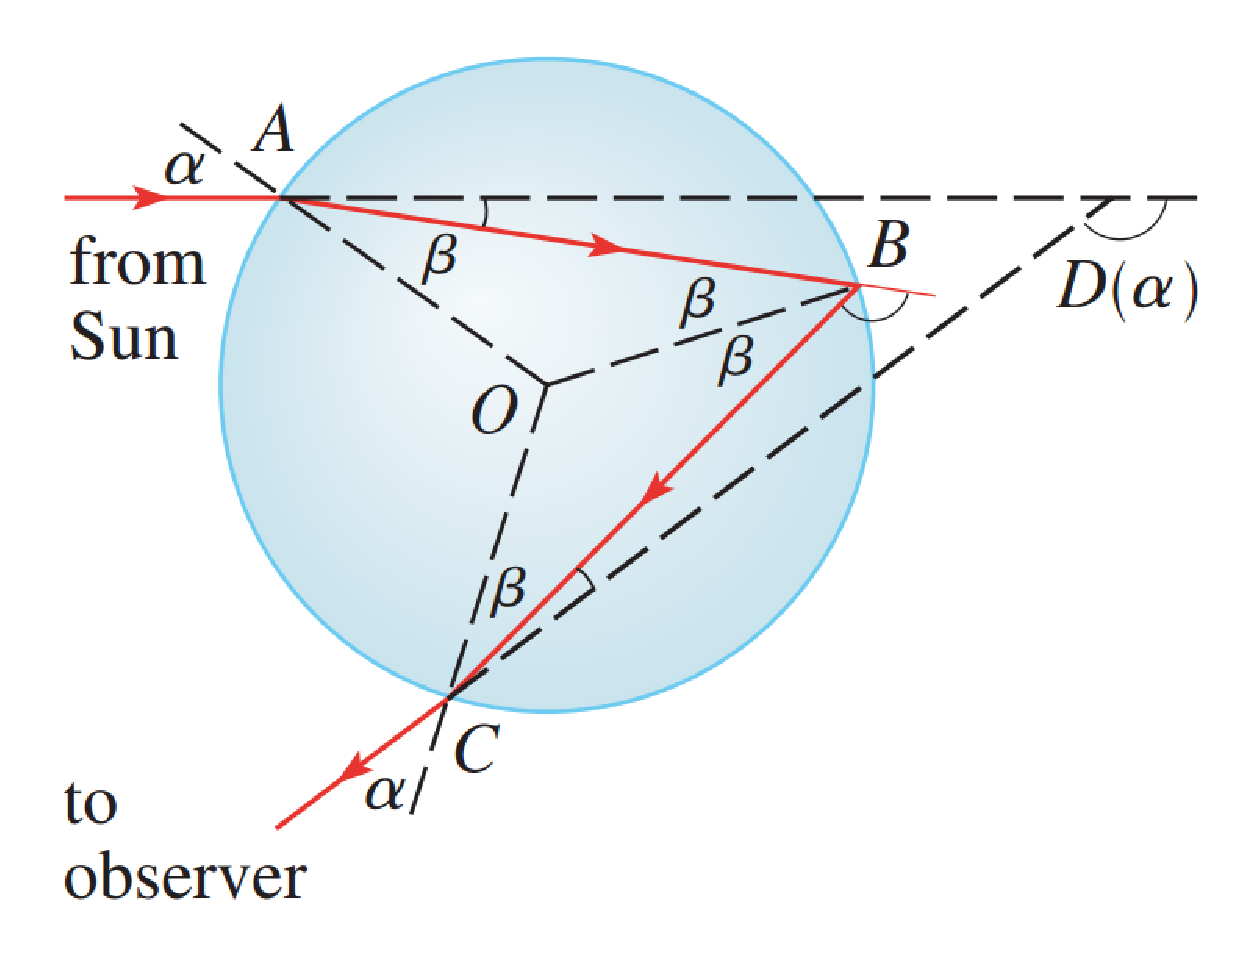
\includegraphics[scale=0.35]{activities/math112/figures/Rainbow.eps}
	\caption{Formation of the primary rainbow.}
	\label{fig:rainbow1}
\end{figure}

Figure \ref{fig:rainbow1} shows a ray of sunlight entering a spherical raindrop at $A$. Some of the light is reflected, but the line $AB$ shows the path of the part that enters the drop. Notice that the light is refracted toward the normal line $AO$ and in fact Snell's Law says that 
\begin{equation}
\label{eq:snellslaw}
\sin(\alpha)=k\sin(\beta),
\end{equation}
\index{mathematical functions!sine}
where $\alpha$ is the angle of incidence, $\beta$ is the angle of refraction, and $k \approx \frac{4}{3}$ is the index of refraction for water. At $B$, some of the light passes through the drop and is refracted into the air, but the line $BC$ shows the part that is reflected. 

\subsection*{Exercises:}
\begin{enumerate}
\item When the ray reaches $C$, part of it is reflected, but for the time being we are more interested in the part that leaves the raindrop at $C$. The angle of deviation $D(\alpha)$\index{greek letter!alpha}\index{greek letter!beta} is the amount of clockwise rotation that the ray has undergone during this three-stage process. The formula for the angle of deviation is given by
\marginnote{The Greek letters alpha ($\alpha$) and beta ($\beta$) can be found on the Greek palette, or typed out and autocompleted using ESC or Ctrl+Space.}
\begin{equation}
\label{eq:deviation1}
D(\alpha)=\pi + 2\alpha -4\beta.
\end{equation}
\clearpage
    \begin{enumerate}
    \marginnote{Make sure to use a lower case $d(\alpha)$ instead of $D(\alpha)$. Maple uses $D$ as a shorthand command for derivatives.}
    \item Solve Equation \eqref{eq:snellslaw} for $\beta$ and substitute this into Equation \eqref{eq:deviation1}.
    \item Show that the minimum value of the deviation is $D(\alpha) \approx 138^{\circ}$ and occurs when $\alpha \approx 59.4^\circ$. 
    \item Plot the Angle of Deviation function in Maple to verify your answer to (b). 
    \end{enumerate}
    \marginnote[-1cm]{You may use the closed interval method over the interval $\alpha \in \left[0,\tfrac{\pi}{2}\right]$. Note that Maple will give you answers in radians, so you will have to convert to degrees. }
\end{enumerate}

The significance of the minimum deviation is that when $\alpha \approx 59.4^\circ$, we have $D'(\alpha)\approx 0$, so $\Delta D/\Delta \alpha \approx 0$. This means that many rays with $\alpha \approx 59.4^\circ$ become deviated by approximately the same amount. It is the concentration of rays coming from near the direction of minimum deviation that creates the brightness of the primary rainbow. Figure \ref{fig:rainbow2} shows that the angle of elevation from the observer up to the highest point on the rainbow is $180^\circ - 138^\circ=42^\circ$. (This angle is called the rainbow angle.) The rainbow angle is found by subtracting the angle of deviation from $180^\circ$ (i.e. $180^\circ - D(\alpha)$).
\marginnote[-2cm]{The rainbow angle is found by \[180^\circ - D(\alpha).\]}
    
\begin{figure}[h]
	\centering
	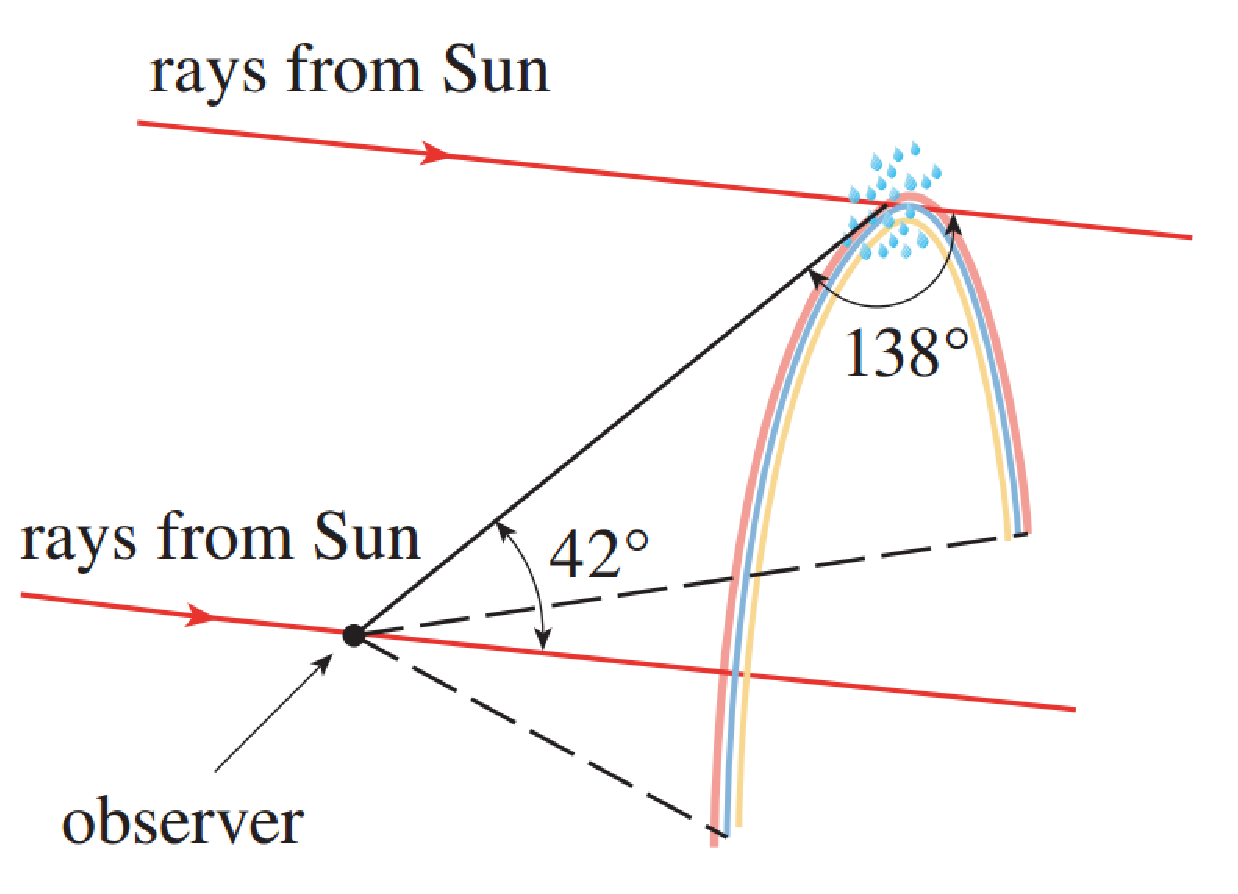
\includegraphics[scale=0.25]{activities/math112/figures/Rainbow2.eps}
	\caption{Angle of elevation from observer.}
	\label{fig:rainbow2}
\end{figure}

Exercise 1 explains the location of the primary rainbow, but how do we explain the colours? Sunlight comprises a range of wavelengths, from the red range through orange, yellow, green, blue, indigo, and violet (ROYGBIV! Ring a bell?). As Newton discovered in his prism experiments of $1666$, the index of refraction is different for each colour. (The effect is called dispersion.)

\begin{enumerate}
\setcounter{enumi}{1}
	\item For red light, the refractive index is $k \approx 1.3318$, whereas for violet light it is $k \approx 1.3435$. By repeating the calculation of exercise 1 for these values of $k$, show that the rainbow angle is about $42.3^\circ$ for the red bow and $40.6^\circ$ for the violet bow. So the rainbow really consists of seven individual bows corresponding to the seven colours.
	\marginnote[-3cm]{In this example, you will repeat exercise 1 using different refractive indices of different colours of light.}
\end{enumerate}

Perhaps you have seen a fainter secondary rainbow above the primary bow. That results from the part of a ray that enters a raindrop and is refracted at $A$, reflected twice (at $B$ and $C$), and refracted as it leaves the drop at $D$ (see Figure \ref{fig:rainbow3}). 
	
\begin{figure}[h]
	\label{fig:rainbow3}
	\centering
	\parbox{0.5\linewidth}{
		\includegraphics[scale=0.25]{activities/math112/figures/Rainbow3.eps}
		\caption{Formation of the secondary rainbow.}
	}
	\hspace{0.05\linewidth}
	\parbox{0.4\linewidth}{
		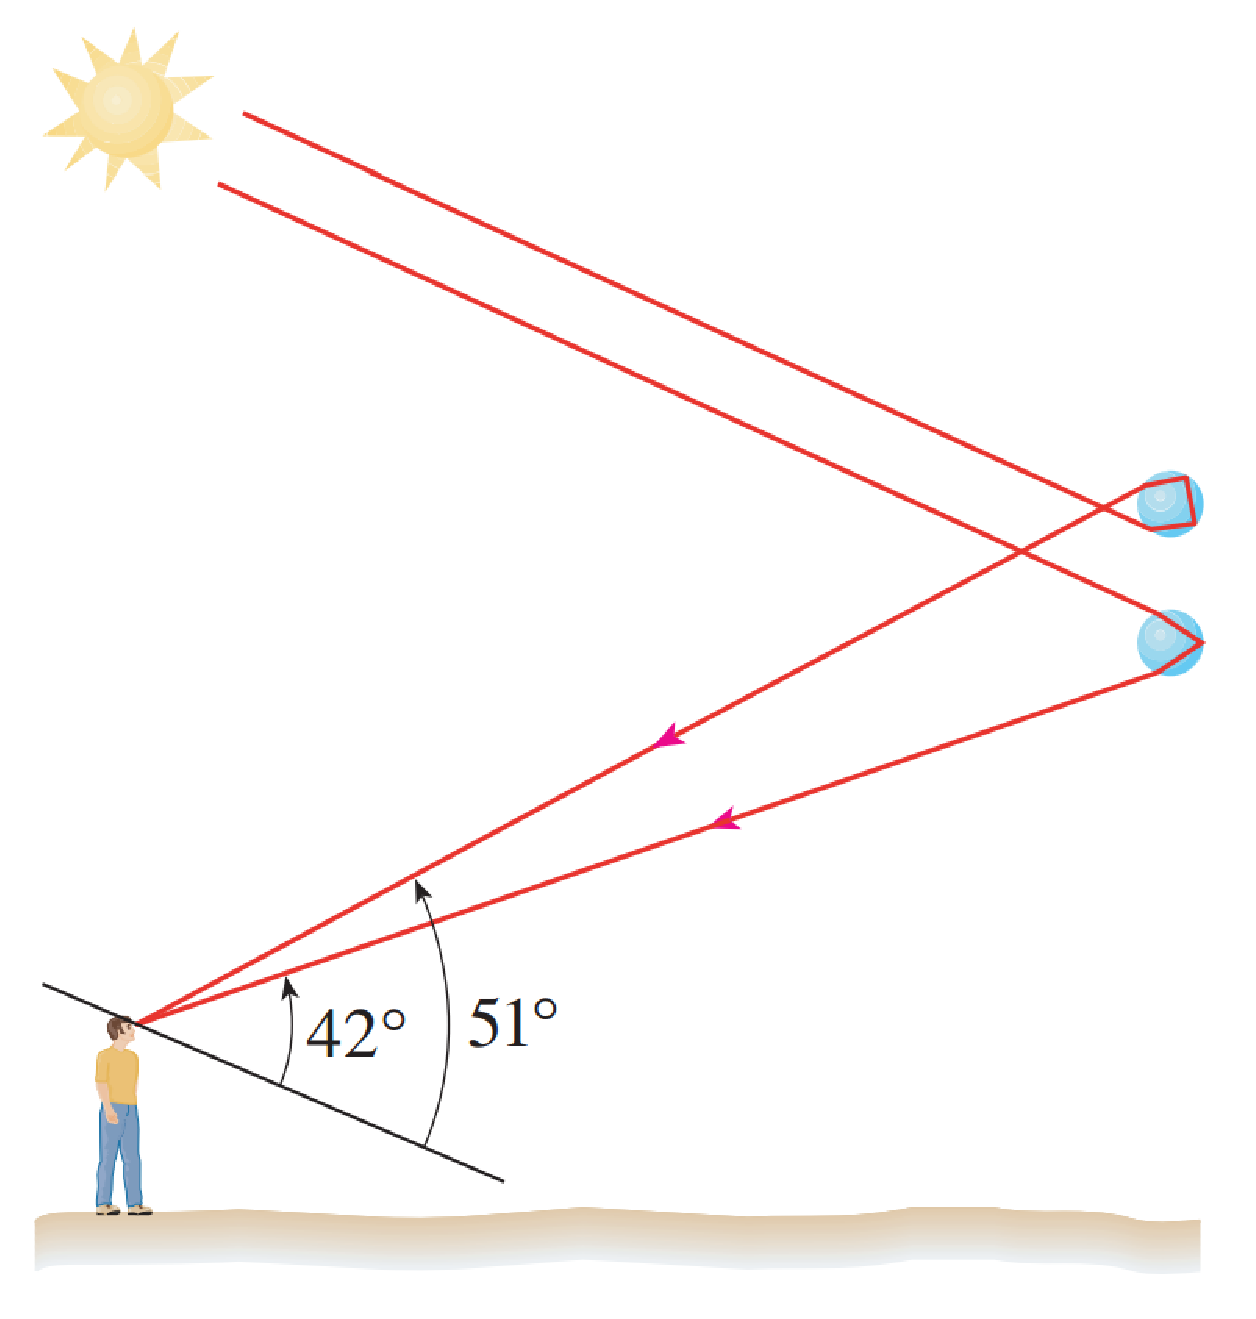
\includegraphics[scale=0.25]{activities/math112/figures/Rainbow4.eps}
		\caption{Angles of elevation from observer.}
	}
\end{figure}

\begin{enumerate}
\setcounter{enumi}{2}	
	\item This time the deviation angle $D(\alpha)$ is the total amount of counterclockwise rotation that the ray undergoes in this four-stage process. In this case, the angle of deviation is given by the formula
\begin{equation}
\label{eq:deviation2}
D(\alpha)=2\alpha-6\beta+2\pi,
\end{equation}
and $D(\alpha)$ has a minimum value when 
\begin{equation}
\label{eq:minvalue}
\cos(\alpha)=\sqrt{\dfrac{k^2-1}{8}}.
\end{equation} \index{mathematical functions!cosine}

\marginnote{It is still necessary to use Snell's Law (Equation \eqref{eq:snellslaw}) to determine the angle of deviation: \[\sin(\alpha)=k\sin(\beta)\]}
	\begin{enumerate}
	\item Solve Equation \eqref{eq:snellslaw} for $\beta$ and substitute this into Equation \eqref{eq:deviation2}. 
	\item When $k \approx \frac{4}{3}$, find the angle of incidence, $\alpha$, using Equation \eqref{eq:minvalue}.
	\item Find the angle of deviation, $D(\alpha)$, using your answers from exercises 3(a) and 3(b).
	\item Verify that the rainbow angle for the secondary rainbow is approximately $51^\circ$, as shown in Figure \ref{fig:rainbow3}.
	\marginnote[-0.5cm]{The rainbow angle is found by \[180^\circ - D(\alpha).\]}
	\end{enumerate}
\end{enumerate}
	

%\subsection*{Notes:}
%\begin{itemize}
%    \item   Use 15 decimal places to find your answers, when applicable.
    
 
%\end{itemize}
\section{Sweet 16}
\label{sec:sweet_16}

\subsection*{Recommended Tutorials:}
\begin{itemize}[noitemsep]
	\item \nameref{chp:equation_solvers}, pg. \pageref{chp:equation_solvers}
	\item \nameref{chp:limits}, pg. \pageref{chp:limits}
	\item \nameref{chp:derivative}, pg. \pageref{chp:derivative}
\end{itemize}

\subsection*{Introduction:}

\marginnote{If we remove the restriction that $a$ and $b$ have to be integers, this problem becomes a lot more interesting. \par It can be shown that for any value $N > {\rm e}^{\rm e}$, there exist real numbers $a$ and $b$ that satisfy $N = a^b = b^a$ with $a \neq b$. To prove this, one needs to be very careful in evaluating the limit \[\lim_{\substack{a \rightarrow 1\\ b \rightarrow \infty}} a^b.\]  It is not obvious that this limit goes to infinity. However, if it does, all $N > {\rm e}^{\rm e}$ will have the desired property. It may help to recall that \[\lim_{n \rightarrow \infty} \left(1 + \frac{1}{n} \right)^n = {\rm e}.\]  So, just because the base tends to $1$ and the exponent tends to infinity, the value of $a^b$ is not necessarily infinity.
}\index{limit}\index{limit!at infinity}\index{limit!definition of e}

We all know that $16$ exhibits the following interesting property: \[16 = 2^4 = 4^2\] Are there any other positive integers $N$ for which there exist positive integers $a$ and $b$ ($a \not = b$) such that \[N = a^b = b^a?\]  This activity will explore this question.

\subsection*{Exercises:}

Let's assume that for some $N \not = 16$, there are positive integers $a$ and $b$ such that $N = a^b = b^a$.

\begin{enumerate}
    \item   If $a^b = b^a$, can we solve for $a$ or $b$?  Why or why not?  Try to do this by hand and comment on the result in a new paragraph.
    \item   Rearrange the equation to separate the $a$'s and $b$'s, so that all $a$'s are on one side and all $b$'s are on the other side. Comment about what you notice about the left and right sides of the equation in a new paragraph.
    \item   Assign the function $f(x) = \ln(x)/x$.  Graph $f(x)$ using Maple.
    \item   Determine the critical point(s) and the maximum and minimum values (if they exist).\index{shapes of curves!critical number}\index{shapes of curves!maximum}\index{shapes of curves!minimum}
    \item   Insert a new paragraph and comment on what happens to $f(x)$ as $x \rightarrow \infty$.\index{shapes of curves!horizontal asymptote}\index{asymptote!horizontal}
    \item   On what intervals is $f(x)$ increasing and decreasing? Answer on a new paragraph.\index{shapes of curves!increasing}\index{shapes of curves!decreasing}
    \marginnote[-2cm]{\textbf{Rolle's Theorem:}\index{Rolle's theorem} Let $f$ be a function that satisfies the following three hypotheses:
    	\begin{enumerate}
    	\item $f$ is continuous on the closed interval $[a,b]$.
    	\item $f$ is differentiable on the open interval $(a,b)$.
    	\item $f(a) = f(b)$.
    	\end{enumerate}
    	Then there is a number $c$ in $(a,b)$ such that $f'(c) = 0$.
    }
    \item   If $f(a) = f(b)$ and $a < b$, what does that mean in terms of the graph? Answer on a new paragraph. \\(\textit{Hint: Rolle's Theorem})
    \item   If $f(a) = f(b)$ and $a < b$, prove that $a = 2$ is the only positive integer such that $a^b = b^a$.
\end{enumerate}

\chapter{Lab Test Review for Math 112}
\label{chp:lab_test_review_math_112}

The following exercises are provided as examples of potential questions on the final lab test at the end of the semester.

\subsection{The Basics}

\begin{enumerate}
\item Evaluate $\sqrt[3]{\dfrac{5.0^2 - 3.0}{1.5 + 9.0^2}}$ to $15$ digits.
\item Give the numerical value of ${\rm e}^2$ to $15$ digits.
\item Factor the given cubic to find its roots.\[ 2x^3 - 7x^2 + 7x -2 \]
\item Find the point of intersection of the curves $y = {\rm e}^x$ and $y = \frac{1}{x}$. Give both the $x$- and $y$-coordinates to $15$ digits.

\subsection{Limits}\index{limit}

\item Find the left- and right-hand limits of  \[ \dfrac{x^2 |x-2|}{x-2} \] at $x=2$. Does the two-sided limit at $x=2$ exist? Explain.
\item Consider the function \[ f(x)=\frac{\sin(x)}{x^2+1}+\arctan(x). \] Evaluate the following limits to $15$ digits.
	\begin{enumerate}
	\item $\dlim{x}{\infty} f(x)$
	\item $\dlim{x}{-\infty} f(x)$
	\end{enumerate}

\subsection{Vertical and Horizontal Asymptotes}\index{asymptote}

\item Sketch the plot of $y=\dfrac{ \sqrt{4x^2 + 1} }{2x - 1}$ and state the equations of vertical and horizontal asymptotes.
\item Find the horizontal asymptote of $\dfrac{5x^3 - 2x + 1}{1 - 8x^3}$.

\subsection{The Derivative of a Function}\index{derivative}

\item Consider the function \[ f(x) = (1-x^2) {\rm e}^{-x^2/2}. \] Find all critical numbers of $f$ to $15$ digits.
\item Consider the function \[ g(x) = \frac{x+2}{3\sqrt{x^2+5}}. \]
	\begin{enumerate}
	\item Plot $g(x)$, $g'(x)$, and $g''(x)$ on the same axes.
	\item Find the maximum value of $g(x)$.
	\item Find the maximum value of $g'(x)$.
	\end{enumerate}
\item The height in metres of a ball thrown from the top of a building is given by the function
\[ h(t) = -9.80t^2 + 5.00t + 40. \]
	\begin{enumerate}
	\item Find the velocity of the ball at $t=2$ seconds.
	\item At what time does the ball reach its maximum height?
	\item What is the maximum height of the ball?
	\end{enumerate}

\subsection{Tangent Lines}\index{lines}

\item Given the function \[ f(x) = {\rm e}^x \cos x, \] find the equation of the tangent line to $f(x)$ at $x=1$ in the form $y = mx + b$.
\item Given the function \[ g(x) = x^{\ln x}, \] find the equation of the tangent line to $g(x)$ at $x=5$ in the form $y = mx + b$.

\subsection{Implicit Functions}\index{implicit functions}

\item Given the Folium of Descartes,
\[ x^3 + y^3 = 6xy, \]
find the slopes of the tangent lines to the curve at $x=2$.
\item Find all points on the curve
\[ (x^2+y^2)^2 = 16(y^2-x^2) \]
where the slope of the tangent line to the curve is equal to $4$.\\
\textit{(Hint: Use the \texttt{fsolve()} command over different intervals to find the required points.)}
\end{enumerate}

\clearpage

\subsection{Solutions}

\begin{enumerate}
    \item $0.643659589737087$
    \item $7.38905609893068$
    \item $\left(x-1\right) \left(x-2\right) \left(2 x-1\right)$
    \item $x= 0.567143290409784, y= 1.76322283435190$
    \item $4$ from the right, $-4$ from the left. No, the two-sided limit at $x = 2$ does not exist because the left and right limits are different.
    \item (a) $1.57079632679490$\\ (b) $-1.57079632679490$
    \item Vertical asymptote: $x=\frac{1}{2}$; Horizontal asymptotes: $y=\pm 1$
    \item $y=-\frac{5}{8}$
    \item $0, 1.73205080756888,- 1.73205080756888$
    \item (b) Maximum value of $0.447213595499958$ at $x=2.5$. \\(c) Maximum value of $0.166566474658809$ at $x=-0.57767710879358$.
    \item (a) $- 34.20$ \\(b) $t=0.255102040816327$ seconds \\(c) $40.6377551020408$ metres
    \item $y=-0.818661347262959 x + 2.28735528717885$
    \item $y=8.58386825467852 x - 29.5856982226701$
    \item $-1.13715804260326, 0.742227198968559, 0.394930843634699$
    \item $(-1.35130857040332, -1.95308486464414)$, $(-1.36235641252506, 2.87932257596956)$, $(1.36235641252506, -2.87932257596956)$, $(1.35130857040332, 1.95308486464414)$
\end{enumerate}

\chapter{Activities for Math 122}
\label{Calc2Activities}

The following list serves as a suggestion for which activities are considered core versus optional:
\begin{table}[h]
\begin{tabular}{lll}
\ref{sec:riemann_sums_for_monotonic_functions}
\nameref{sec:riemann_sums_for_monotonic_functions}			& pg. \pageref{sec:riemann_sums_for_monotonic_functions}		& Core\\
\ref{sec:visualizing_the_net_change_theorem}
\nameref{sec:visualizing_the_net_change_theorem}			& pg. \pageref{sec:visualizing_the_net_change_theorem}			& Core\\
\ref{sec:approximate_integration}
\nameref{sec:approximate_integration}						& pg. \pageref{sec:approximate_integration}						& Optional\\
\ref{sec:max_and_min_problems_for_integrals}
\nameref{sec:max_and_min_problems_for_integrals}			& pg. \pageref{sec:max_and_min_problems_for_integrals}			& Optional\\
\ref{sec:applications_of_ftc}
\nameref{sec:applications_of_ftc}							& pg. \pageref{sec:applications_of_ftc}							& Optional\\
\ref{sec:average_value_of_function}
\nameref{sec:average_value_of_function}						& pg. \pageref{sec:average_value_of_function}					& Optional\\
\ref{sec:shark_attack}
\nameref{sec:shark_attack}									& pg. \pageref{sec:shark_attack}								& Optional\\
\ref{sec:area_problem}
\nameref{sec:area_problem}									& pg. \pageref{sec:area_problem}								& Core\\
\ref{sec:volumes_of_revolution}
\nameref{sec:volumes_of_revolution}							& pg. \pageref{sec:volumes_of_revolution}						& Optional\\
\ref{sec:golden_gate_bridge_problem}
\nameref{sec:golden_gate_bridge_problem}					& pg. \pageref{sec:golden_gate_bridge_problem}					& Optional\\
\ref{sec:infinite_integrals}
\nameref{sec:infinite_integrals}							& pg. \pageref{sec:infinite_integrals}							& Core\\
\ref{sec:probability}
\nameref{sec:probability}									& pg. \pageref{sec:probability}									& Optional\\
\ref{sec:motion_of_a_mass_connected_to_a_spring}
\nameref{sec:motion_of_a_mass_connected_to_a_spring}		& pg. \pageref{sec:motion_of_a_mass_connected_to_a_spring}		& Optional$^1$\\
\ref{sec:tank_mixing_problem}
\nameref{sec:tank_mixing_problem}							& pg. \pageref{sec:tank_mixing_problem}							& Optional$^1$\\
\ref{sec:direction_fields}
\nameref{sec:direction_fields}								& pg. \pageref{sec:direction_fields}							& Optional$^1$\\
\ref{sec:series_convergence_and_divergence}
\nameref{sec:series_convergence_and_divergence}				& pg. \pageref{sec:series_convergence_and_divergence}			& Core\\
\ref{sec:taylor_series}
\nameref{sec:taylor_series}									& pg. \pageref{sec:taylor_series}								& Core\\
%\ref{sec:approximations_of_pi}
%\nameref{sec:approximations_of_pi}							& pg. \pageref{sec:approximations_of_pi}						& Optional
\\
\multicolumn{3}{l}{$^1$One of these activities covering differential equations should be chosen as core.}
\end{tabular}
\end{table}

\section{Riemann Sums for Monotonic Functions}
\label{sec:riemann_sums_for_monotonic_functions}		

\subsection*{Recommended Tutorials:}
\begin{itemize}[noitemsep]
    \item \nameref{chp:limits}, pg. \pageref{chp:limits}
	\item \nameref{chp:riemann_sums_and_area_approximation}, pg. \pageref{chp:riemann_sums_and_area_approximation}
\end{itemize}

\subsection*{Introduction:}

A monotonic function is one that is strictly increasing or strictly decreasing. In this activity, we will use Maple's \texttt{ApproximateInt()} command to visualize and calculate Riemann sums\index{integral approximation!Riemann sum} for the area below the monotonic function \[ f(x) = x - 2\ln(x).\]
\index{integral approximation!ApproximateInt}
\marginnote{You will need to load the \texttt{Student[Calculus1]}\index{packages!Student[Calculus1]} package to use the \texttt{ApproximateInt()} command. You can do this by typing \texttt{with(Student[Calculus1]):} at the start of your worksheet.}
\index{integral approximation!ApproximateInt!method}\index{integral approximation!ApproximateInt!output options}

\subsection*{Exercises:}

\marginnote[1cm]{Using left and right endpoint methods, it is easy to come up with an overestimate and underestimate for monotonic functions.  In particular, to come up with an overestimate requires only one Riemann sum calculation.}
\begin{enumerate}
    \item Use the \texttt{ApproximateInt()} command for \[f(x) = x - 2\ln(x)\] on the interval $[2,10]$ with $10$ partitions.
        \index{integral approximation!ApproximateInt!partition}
    \begin{enumerate}
        \item Use the options \texttt{method=left} and \texttt{output=plot}.
        \item Repeat the command, but using \texttt{method=right} and \texttt{output=plot}.
    \end{enumerate}
\end{enumerate}
For exercises $2$ through $5$, answer the question in a new paragraph on your Maple worksheet.
\begin{enumerate}
	\setcounter{enumi}{1}
    \item   What do you notice about using the left-point method to estimate the area below a monotonically increasing function?
    \item   What do you notice about using the right-point method to estimate the area below a monotonically increasing function?
    \item   What do you suspect will happen if you use the left-point method to estimate the area below a monotonically decreasing function?
    \item   What do you suspect will happen if you use the right-point method to estimate the area below a monotonically decreasing function?
    \item   Repeat Exercise $1$, but change \texttt{output=plot} to \texttt{output=value}\index{integral approximation!ApproximateInt!output options}. Evaluate these areas to $15$ digits.
    \marginnote[-2cm]{Don't forget that you can convert an exact value to decimal using the \texttt{evalf()}\index{evalf} command. You can set the accuracy to $15$ digits at the top of your worksheet using the command \texttt{Digits := 15}. Note that the first letter is always capitalized in \texttt{Digits}.}\index{Digits}
    \item   Using $n$ partitions and \texttt{output=sum}, give the Riemann sum for $f(x)$ on the interval $[2,10]$. Use both left- and right-point methods.  What happens as $n \rightarrow \infty$?
    \item   Estimate the Riemann sum for $f(x)$ on the interval $[0.5, 3]$ using $10$ boxes and left- and right-point methods.  What do you notice about your answers?  Does this contradict your findings about monotonic functions?
    \marginnote[-1.5cm]{Any function that is not monotonic is not as easy to find an overestimate or underestimate for.}
\end{enumerate}


\section{The Net Change Theorem}
\label{sec:visualizing_the_net_change_theorem}

\subsection*{Recommended Tutorials:}
\begin{itemize}[noitemsep]
    \item \nameref{chp:limits}, pg. \pageref{chp:limits}
    \item \nameref{chp:riemann_sums_and_area_approximation}, pg. \pageref{chp:riemann_sums_and_area_approximation}
	\item \nameref{chp:definite_and_indefinite_Integrals}, pg. \pageref{chp:definite_and_indefinite_Integrals}
\end{itemize}

\subsection*{Introduction:}

The Net Change\index{integral!net change} Theorem states that if a quantity $Q = F(t)$ is a differentiable function on the interval $[a,b]$, then 
\begin{align*}
	\int_{a}^b F'(t) \; dt 
	&= F(b) - F(a) \\
	&= \text{ net change in } Q \text{ over } [a,b].
\end{align*}
    \index{integral!}
In other words, the Net Change Theorem states that the definite integral of the rate of change of $Q$ from $a$ to $b$ is given by the difference in the initial quantity and the final quantity.

We may also be interested in finding the total change of the quantity $Q$, given by the integral
\[
	\int_{a}^{b} |F'(t)| dt.
\]
\index{integral!total change}
In this case, all area is positive. 

We will use Maple's \texttt{ApproximateInt()}\index{integral approximation!ApproximateInt} command to help visualize the net change and total change of a function. In addition to the \texttt{method=left}\index{integral approximation!ApproximateInt!method} and \texttt{method=right} parameters, we can also use \newline\noindent\texttt{method=upper} and \texttt{method=lower} to ensure that our approximation is an overestimate or an underestimate, respectively.
\marginnote[-2cm]{You will need to load the \texttt{Student[Calculus1]}\index{packages!Student[Calculus1]} package to use the \texttt{ApproximateInt()} command. You can do this by typing \texttt{with(Student[Calculus1]):} at the start of your worksheet.}

\subsection*{Exercises:}

\begin{enumerate}
    \item   Define the function $f(x) = \dfrac{x}{x^2+4}$.  Plot $f(x)$ on the interval $[-5,10]$.
    \item   Use the \texttt{ApproximateInt()}\index{integral approximation!ApproximateInt!method} command to calculate the \textit{net} change of $f(x)$ on the interval $[-5,10]$ with $15$ partitions. Use both\\ \texttt{method=upper} and \texttt{method=lower}.
    \item   Use the \texttt{ApproximateInt()} command with \texttt{method=right} and $n$ partitions to give the Riemann sum for $f(x)$ on the interval $[-5,10]$.  Use the \texttt{limit()}\index{limit} command to find the limit of this value as $n$ goes to infinity. You may need to use the \texttt{value(\%)} command in order to get a numerical value.
    \marginnote[-1cm]{This \texttt{value(\%)}\index{value}\index{ditto operator} command will force Maple to evaluate the limit and produce a numerical value.}
    \item   Compute $\displaystyle\int_{-5}^{10} f(x) \; dx$ by using the \texttt{Int()} command.  Verify that this value matches the limit of the Riemann sum in the previous exercise.
    \item   Use the \texttt{ApproximateInt()}\index{integral approximation!ApproximateInt} command to calculate the \textit{total} change\index{integral!total change} of $f(x)$ on the interval $[-5,10]$ with $15$ partitions. Use both\\ \texttt{method=upper} and \texttt{method=lower}.\index{integral approximation!ApproximateInt!method}
    \marginnote{Recall that the \texttt{abs()}\index{mathematical functions!absolute value} command is used for absolute values in Maple.}
    \item   Use the \texttt{ApproximateInt()} command with \texttt{method=right} and $n$ partitions to give the Riemann sum\index{integral approximation!Riemann sum} for $|f(x)|$ on the interval $[-5,10]$.  Use the \texttt{limit()}\index{limit} command to find the limit of this value as $n$ goes to infinity. You may need to use the \texttt{value(\%)}\index{value}\index{ditto operator} command in order to get a numerical value.
    \item    Compute $\displaystyle\int_{-5}^{10} |f(x)| \; dx$ by using the \texttt{Int()} command\index{integral!Int}.  Verify that this value matches the limit of the Riemann sum in the previous exercise.
    \marginnote[-1.5cm]{Think about how you would evaluate this integral if you could not integrate the absolute value function.  In general, computing $\displaystyle\int_{a}^b \abs{f(x)} \, dx$ is difficult.}
    \item   In a new paragraph, describe the difference between the net area and the total area bounded by the function $f(x)$ and the $x$-axis on the interval $[-5,10]$.
    \marginnote[-1cm]{The net area and the total area between a curve and the $x$-axis can be different quantities.  It is important to know when they are different and when they are the same.}\index{integral!net change}
\end{enumerate}

\section{Other Integral Approximation Techniques}
\label{sec:approximate_integration}	

\subsection*{Recommended Tutorials:}
\begin{itemize}[noitemsep]
    \item \nameref{chp:derivative}, pg. \pageref{chp:derivative}
	\item \nameref{chp:riemann_sums_and_area_approximation}, pg. \pageref{chp:riemann_sums_and_area_approximation}
\end{itemize}

\subsection*{Introduction:}

The trapezoid rule, the midpoint rule, and Simpson's rule are all useful methods for approximating a definite integral of a function $f(x)$. However, each of these methods has some error in its approximation for a finite number of subintervals. It is possible to calculate an upper bound for this error, which relies on calculating the the maximum value of $|f''(x)|$ (or $|f^{(4)}(x)|$ for Simpson's rule) over the interval first.

In this activity, we will use Maple's \texttt{ApproximateInt()}\index{integral approximation!ApproximateInt} command to help visualize these three approximation methods and then calculate the error associated with them.

\subsection*{Exercises:}

Consider the definite integral $\displaystyle\int_{0}^1 {\rm e}^x\sin(x) \; dx$.\index{integral!}

\begin{enumerate}
    \item   Plot ${\rm e}^x\sin(x)$ on the interval $[0,1]$.
    \marginnote{Don't forget that the \texttt{exp()}\index{mathematical functions!exponential} function is used for ${\rm e}^x$. You cannot use the letter `e' on the keyboard for the exponential function.}
    \item   Consider the area under ${\rm e}^x\sin(x)$ using the \textbf{trapezoid} rule with \\ \texttt{partition=4} over the interval $[0,1]$.\index{integral approximation!ApproximateInt!method}
        \index{integral approximation!ApproximateInt!partition}
    \begin{enumerate}
    	\item Display this area using \texttt{output=plot}.
    	    \index{integral approximation!ApproximateInt!output options}
    	\item Display the sum for this area using \texttt{output=sum}.
    	\item Find the value of this area using \texttt{output=value}.
    \end{enumerate}
    \item   Consider the area under ${\rm e}^x\sin(x)$ using the \textbf{midpoint} rule with \\ \texttt{partition=4} subintervals over the interval $[0,1]$.\index{integral approximation!ApproximateInt!method}
    \begin{enumerate}
    	\item Display this area using \texttt{output=plot}.
    	\item Display the sum for this area using \texttt{output=sum}.
    	\item Find the value of this area using \texttt{output=value}.
    \end{enumerate}
    \item   Consider the area under ${\rm e}^x\sin(x)$ using \textbf{Simpson's} rule with \\ \texttt{partition=4} subintervals over the interval $[0,1]$.\index{integral approximation!ApproximateInt!method}
    \begin{enumerate}
    	\item Display this area using \texttt{output=plot}.
    	\item Display the sum for this area using \texttt{output=sum}.
    	\item Find the value of this area using \texttt{output=value}.
    \end{enumerate}
    \item The upper bounds for the errors of the \textbf{trapezoid} and \textbf{midpoint} rules over the interval $[a,b]$ are 
    \[\abs{E_T}\le\dfrac{K(b-a)^3}{12n^2} \quad\text{and}\quad \abs{E_M}\le\dfrac{K(b-a)^3}{24n^2},\] respectively. In both cases, $K$ is the maximum value of $\abs{f''(x)}$ over the interval and $n$ is the number of subintervals. Compute these error bounds by following the steps listed.
        \index{integral approximation!error}
    \begin{enumerate}
        \item Plot $|f''(x)|$ over the interval $[0,1]$. Notice that the maximum value of $|f''(x)|$ occurs at a critical number of $|f''(x)|$.
        \item Find the critical number of $|f''(x)|$ by solving $f'''(x)=0$ for $x$. Plug this $x$-value back into $|f''(x)|$ to find the maximum, $K$.
        \item Compute $|E_T|$ using the formula, $K$, and $n=4$.
        \item Compute $|E_M|$ using the formula, $K$, and $n=4$.
    \end{enumerate}
    \marginnote[1cm]{When using Simpson's rule with \texttt{partition=4}, this actually correponds to $n=8$, since there is an additional sample point in each partition.}
    \item  The upper bound for error of \textbf{Simpson's} rule over the interval $[a,b]$ is \[\abs{E_S}\le\dfrac{K(b-a)^5}{180n^4}\] where $\abs{f^{(4)}(x)}\le K$ and $n$ is \textbf{twice} the number of subintervals. Compute this error bound by following the steps listed.
    \index{integral approximation!error}
    \begin{enumerate}
        \item Plot $|f^{(4)}(x)|$ over the interval $[0,1]$. Notice that the maximum value of $|f^{(4)}(x)|$ occurs at an endpoint of the interval.
        \item Plug the $x$-value of this endpoint into $|f^{(4)}(x)|$ to find the maximum, $K$.
        \item Compute $|E_S|$ using the formula, $K$, and $n=8$.
    \end{enumerate}
\end{enumerate}

\section{Describing the Shapes of Integral Functions}
\label{sec:max_and_min_problems_for_integrals}	

\subsection*{Recommended Tutorials:}
\begin{itemize}[noitemsep]
	\item \nameref{chp:assignment_operator}, pg. \pageref{chp:assignment_operator}
	\item \nameref{chp:equation_solvers}, pg. \pageref{chp:equation_solvers}
	\item \nameref{chp:limits}, pg. \pageref{chp:limits}
	\item \nameref{chp:derivative}, pg. \pageref{chp:derivative}
	\item \nameref{chp:definite_and_indefinite_Integrals}, pg. \pageref{chp:definite_and_indefinite_Integrals}
\end{itemize}

\subsection*{Introduction:}

\marginnote[1cm]{Recall that a critical point of a function $f(x)$ occurs when $f'(x) = 0$ or when $f'(x)$ does not exist.} 
    \index{shapes of curves!critical number}
\marginnote[1cm]{An inflection point of $f(x)$ is a point at which the concavity of $f(x)$ changes.}
    \index{shapes of curves!inflection point}
In this activity, we will examine two functions that are defined by integrals, in the form
\[ f(x) = \int_0^x g(t) \, dt.\] 
    \index{integral!}
We may view these integral functions as the accumulated area under the function $g(t)$ over an interval from $0$ to $x$. Integral functions frequently appear in analysis and in differential equations.  Determining critical points and inflection points is incredibly important in the analysis of these types of problems.

\subsection*{Exercises:}

\begin{enumerate}
    \item The sine integral function
    \[Si(x) = \begin{cases} \displaystyle\int_{0}^x \dfrac{\sin(t)}{t}\, dt & x \neq 0 \\ 1 & x = 0 \end{cases}\]
        \index{mathematical functions!piecewise}
    is important in electrical engineering. By defining $Si(0)=1$ in the piecewise definition above, $Si(x)$ is a continuous function.
    \begin{enumerate}
        \item The sine integral function is already defined in Maple by typing \texttt{Si(x)}. Plot\index{plot} the graph of $Si(x)$ over the interval $[-15,15]$.
        \marginnote[.2cm]{When you use the \texttt{fsolve()}\index{solving equations!fsolve} command, you can specify an interval in which you wish to search for solutions. An example of this can be found on page \pageref{eg:fsolve_interval}.}
        \item On the graph of $Si(x)$, you will notice that there are many local minimum and maximum values. Use the \texttt{fsolve()} command to find the critical numbers\index{shapes of curves!critical number} of $Si(x)$ corresponding to the location of the absolute minimum and maximum values.
        \index{shapes of curves!minimum}
        \index{shapes of curves!maximum}
        \item What are the absolute minimum and maximum values of $Si(x)$?
        \marginnote[-1.cm]{By the Fundamental Theorem of Calculus, \[\dfrac{d}{dx} Si(x) = \dfrac{\sin(x)}{x} = \text{sinc}(x)\] ($x \not = 0$).  This function is used in signal processing and the theory of Fourier transforms.}
        \vspace{-.5cm}
        \item There is an inflection point just to the right of the absolute maximum value. Use the second derivative $Si''(x)$ and the \texttt{fsolve()} command to find its location.
        \index{shapes of curves!inflection point}
        \index{solving equations!fsolve}
        \marginnote[.4cm]{Recall that if \[\lim_{x\rightarrow\infty} f(x) = L ~\text{or}~ \lim_{x\rightarrow-\infty} f(x) = L\] and $L$ is finite, then $y=L$ is a horizontal asymptote of $f(x)$.}
        \item Use the \texttt{limit()} command to find the horizontal asymptote(s) of $Si(x)$.
            \index{limit}
            \index{asymptote!horizontal}
    \end{enumerate}
    \item   Consider the integral function: \[f(x) = \displaystyle\int_{0}^x \dfrac{1}{1 + t + t^2} \, dt.\]
        \index{integral!}
    \begin{enumerate}
        \item Define $f(x)$ in Maple.
        \item Plot\index{plot} the integral function, $f(x)$. Try to specify a plot interval that gives you a good idea of the shape of $f(x)$.
        \item Use the second derivative\index{derivative}, $f''(x)$, to determine where $f(x)$ is concave up and where $f(x)$ is concave down.
        \item Determine the inflection points of $f(x)$.
            \index{shapes of curves!inflection point}
    \end{enumerate}
\end{enumerate}

\section{Applications of the Fundamental Theorem of Calculus}
\label{sec:applications_of_ftc}			

\subsection*{Recommended Tutorials:}
\begin{itemize}[noitemsep]
	\item \nameref{chp:limits}, pg. \pageref{chp:limits}
	\item \nameref{chp:equation_solvers}, pg. \pageref{chp:equation_solvers}
	\item \nameref{chp:derivative}, pg. \pageref{chp:derivative}
	\item \nameref{chp:definite_and_indefinite_Integrals}, pg. \pageref{chp:definite_and_indefinite_Integrals}
\end{itemize}

\subsection*{Introduction:}

In this activity, you will need to make use of the Fundamental Theorem of Calculus in order to solve two applied problems. In particular, you will need to use the result \[ \frac{d}{dx} \int_a^x f(t) \, dt = f(x). \]
    \index{integral!}

\vspace{-.5cm}
\subsection*{Exercises:}

\begin{enumerate}        
    \item In this exercise, our goal is to evaluate $\displaystyle\lim_{x \rightarrow 0} \dfrac{\int_{0}^x \sin(t^2) \; dt}{x^3}.$
\index{limit}
        \index{plot}
        \index{limit!l'H\^opital}
    \begin{enumerate}
        \marginnote[1cm]{L'H\^opital's Rule states that if the limit \[\lim_{x\rightarrow a}\frac{f(x)}{g(x)}\] is indeterminate of the form $0/0$ or $\infty/\infty$, if $f$ and $g$ are differentiable at $a$, and if $g'(x) \neq 0$ near $a$, then \[\lim_{x\rightarrow a}\frac{f(x)}{g(x)} = \lim_{x\rightarrow a}\frac{f'(x)}{g'(x)},\] assuming that this limit exists.}
        \item Define the function $s(x) = \dfrac{\int_{0}^x \sin(t^2) \; dt}{x^3}$.  Plot the graph of $s(x)$ over the interval $[-1,1]$. Try to estimate $\displaystyle\lim_{x\rightarrow0}s(x)$.
        \item Is there an easy integration technique that you could use to integrate $\displaystyle\int_{0}^x \sin(t^2) \; dt$ by hand?  If not, why?
        \item What is the indeterminate form of the limit?
        \item Apply L'H\^opital's Rule by hand, in the space below. Check your answer by using the \texttt{limit()} command to evaluate $\displaystyle\lim_{x\rightarrow0}s(x)$.
    \end{enumerate}
    \begin{fullwidth}
    \fbox{\parbox{1\linewidth}{$\displaystyle\lim_{x \rightarrow 0} \dfrac{\displaystyle\int_{0}^x \sin(t^2) \; dt}{x^3}=$ \vspace{6cm} }}
    \end{fullwidth}
\clearpage
    \item In this exercise, our goal is to find a function $f$ and a number $a$ that satisfy the equation 
    \begin{equation}
        \label{eq:ftc_equation}
        6 + \displaystyle\int_{a}^x \dfrac{f(t)}{t^2} dt = 2\sqrt{x}.
    \end{equation}
    \begin{enumerate}
        \item Assign equation \eqref{eq:ftc_equation} to a name of your choice, such as \texttt{eqn}.
        \marginnote[0.5cm]{The \texttt{diff()}\index{derivative!diff} command can be used to differentiate an equation with respect to an independent variable.}
        \item In the space below, differentiate both sides of the equation with respect to $x$ and apply the Fundamental Theorem of Calculus. Check your answer by using the \texttt{diff()} command on the equation you assigned in the previous step.
        \begin{fullwidth}
        \fbox{\parbox{1\linewidth}{\[6 + \displaystyle\int_{a}^x \dfrac{f(t)}{t^2} dt = 2\sqrt{x}\] \vspace{3cm} }}
        \end{fullwidth}
     \index{solving equations!solve}
        \item Solve the resulting equation for $f(x)$ using the \texttt{solve()} command. 
        \item Replace $f(t)$ in equation \eqref{eq:ftc_equation} with the function that you solved for in part (c). Make sure to use $t$ as the variable. Assign this to a new name in Maple.
        \item Evaluate the integral in the equation and solve for $a$ in Maple.
    \end{enumerate}
\end{enumerate}
\section{Average Value of a Function on a Shrinking Interval}
\label{sec:average_value_of_function}	

\subsection*{Recommended Tutorials:}
\begin{itemize}[noitemsep]
	\item \nameref{chp:limits}, pg. \pageref{chp:limits}
	\item \nameref{chp:definite_and_indefinite_Integrals}, pg. \pageref{chp:definite_and_indefinite_Integrals}
\end{itemize}

\subsection*{Introduction:}

The average value of a function\index{average value of a function} $f$ on the interval $[a,b]$ is defined as 
\[ f_{ave} = \frac{1}{b-a} \int_{a}^{b} f(x) \, dx. \]
In this activity, we will investigate the function 
\[ f(x) = \sqrt{1 + x^3} \]
over a shrinking interval where $a = 2$ fixed and $b$ approaches $a$. To do this, we can let $b=2+h$ and take the limit as $h \rightarrow 0$. Specifically, we will determine the value of the integral
\[\displaystyle\lim_{h \rightarrow 0} \dfrac{1}{h} \displaystyle\int_{2}^{2+h} \sqrt{1 + x^3}\, dx.\]
For convenience, we can view 
\[avg(h) = \frac{1}{h}\displaystyle\int_{2}^{2+h} \sqrt{1 + x^3}\, dx\]
as a function of $h$. This function gives the average value of \\\noindent $f(x) = \sqrt{1 + x^3}$ over the interval $[2,2+h]$.

\subsection*{Exercises:}

\begin{enumerate}
    \marginnote{Note that you should use $h$ as the independent variable of this function.}
    \item Assign the function $avg(h) = \dfrac{1}{h} \displaystyle\int_{2}^{2+h} \sqrt{1 + x^3}\, dx$.
    \item Use this function to find the average value of $f(x) = \sqrt{1+x^3}$ on the interval $[2,4]$.
    \item Plot\index{plot} $avg(2)$ and $\sqrt{1+x^3}$ on the same axes over the interval $[2,4]$. Does $avg(2)$ appear to be the average value of $f(x) = \sqrt{1+x^3}$ on the interval $[2,4]$?
    \item Plot $avg(h)$ over the interval $h\in[-1,1]$. Estimate the value $\displaystyle\lim_{h \rightarrow 0} \dfrac{1}{h} \displaystyle\int_{2}^{2+h} \sqrt{1 + x^3}\, dx$ from your graph.
    \item Is there an easy integration technique that you could use to integrate $\displaystyle\int_{2}^{2+h} \sqrt{1 + x^3}\, dx$ by hand? If not, why?
    \item Determine $\displaystyle\lim_{h \rightarrow 0} \dfrac{1}{h} \displaystyle\int_{2}^{2+h} \sqrt{1 + x^3} \,dx$ by hand using L'H\^opital's Rule in the space below. Make sure to state the indeterminate form. 
    \label{ex:average_value_limit}
    \marginnote[-.7cm]{L'H\^opital's Rule states that if the limit \[\lim_{x\rightarrow a}\frac{f(x)}{g(x)}\] is indeterminate of the form $0/0$ or $\infty/\infty$, if $f$ and $g$ are differentiable at $a$, and if $g'(x) \neq 0$ near $a$, then \[\lim_{x\rightarrow a}\frac{f(x)}{g(x)} = \lim_{x\rightarrow a}\frac{f'(x)}{g'(x)},\] assuming that this limit exists.}
    \index{limit!l'H\^opital}
    \par
    \fbox{\parbox{1\linewidth}{$\displaystyle\lim_{h \rightarrow 0} \dfrac{\displaystyle\int_{2}^{2+h} \sqrt{1 + x^3} \,dx}{h}=$ \vspace{8cm} }}
    \item Check your answer to question \ref{ex:average_value_limit} by using the \texttt{limit()} command to evaluate $\displaystyle\lim_{h\rightarrow0}avg(h)$.
        \index{limit}
\end{enumerate}


\section{Shark Attack}
\label{sec:shark_attack}	

\subsection*{Recommended Tutorials:}
\begin{itemize}[noitemsep]
	\item \nameref{chp:assignment_operator}, pg. \pageref{chp:assignment_operator}
	\item \nameref{chp:equation_solvers}, pg. \pageref{chp:equation_solvers}
	\item \nameref{chp:definite_and_indefinite_Integrals}, pg. \pageref{chp:definite_and_indefinite_Integrals}
\end{itemize}

\subsection*{Introduction:}

In this activity, you will determine whether you can swim to safety before a shark attacks. You will need to use piecewise functions and the Net Change Theorem to find the outcome. 

\tikzset{
   ragged border/.style={ decoration={random steps, segment length=1mm, amplitude=0.5mm},
           decorate,
   }
}
\begin{figure}[h]
\centering
\begin{tikzpicture}
    \fill[cyan!30] decorate[ragged border]{ (0,2) -- (8,2) } -- (8,0) -- (0,0) -- cycle;
    \fill[yellow!30] decorate[ragged border]{ (8,2) -- (8,0) } -- (9,0) -- (9,2) -- cycle;
    \draw (1.5,1) node {\scalebox{-0.2}[0.2]{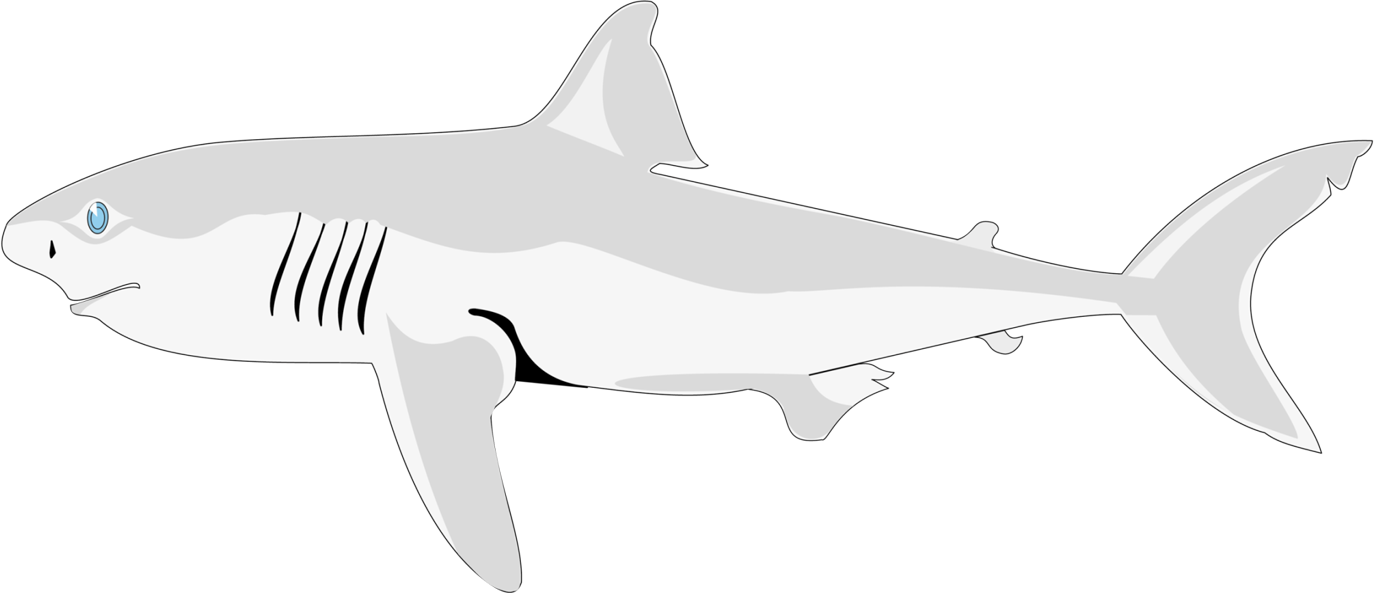
\includegraphics{activities/math122/figures/shark.png}}};
    \draw (5,1) node {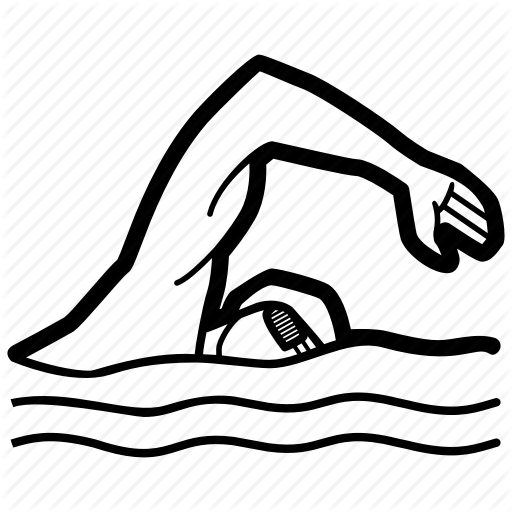
\includegraphics[scale=0.075]{activities/math122/figures/swimmer.png}};
    \draw[|-|] (1.5,3) node [above] {$\SI{0}{m}$} -- (5,3) node [above] {$\SI{50}{m}$};
    \draw[|-|] (5,3) -- (8,3) node [above] {$\SI{70}{m}$};
\end{tikzpicture}
\caption{An illustration of the shark trying to catch you as you swim to shore.}
\label{fig:shark_attack}
\end{figure}

Suppose that you are surfing on the ocean and there is a shark $\SI{50}{m}$ behind you, at rest (i.e. $v(0)=0$). \\

The shark senses you and begins accelerating toward you at a rate of $\SI{5}{m/s^2}$, up to a top speed of $\SI{13}{m/s}$.
You see the shark coming and begin swimming towards shore at a speed of $\SI{2}{m/s}$. Assume there is no time needed for you to accelerate up to your top speed. If the shore is $\SI{20}{m}$ away from you (and $\SI{70}{m}$ away from the shark), do you make it to shore before the shark attacks?

\begin{marginfigure}[-2cm]
\centering
\begin{tikzpicture}
\begin{axis}[
	width=\textwidth,
	height=0.8\textwidth,
	clip=false,
	axis lines=middle,
	xlabel={$t$},
	ylabel={$v$},
	xlabel style={below right},
	ylabel style={above left},
	xmin=-0.5, xmax=8, xtick={0},
	ymin=-2, ymax=15, ytick={0,13}
]
	\addplot [domain=0:2.6, samples=100] {5*x};
	\addplot [domain=2.6:8, samples=100] {13};
	\draw [dashed] (axis cs:2.6,13) -- (axis cs:2.6,0);
	\draw (axis cs:2.6,0) node [below] {$t_1$};
\end{axis}
\end{tikzpicture}
\caption{The shark speeds up to its top speed of $\SI{13}{m/s}$ with a constant acceleration of $\SI{5}{m/s^2}$. This results in a piecewise defined function $v(t)$ shown here.}
\label{fig:sharkvelocity}
\end{marginfigure}

\subsection*{Exercises:}

\begin{enumerate}
    \item Calculate the time $t_1$ it takes for the shark to reach its top speed of $13$ m/s if it accelerates at $5$ m/s\textsuperscript{2}. Note that the shark will no longer accelerate after $t_1$ seconds, since it has reached its top speed. \label{ex:sharktime}
    \marginnote[-1.5cm]{The shark's velocity will contain an acceleration term for $0 \le t \le t_1$ (where $t_1$ is the time you find in exercise \ref{ex:sharktime}) but will not have an acceleration term after $t_1$ seconds.}
    \item Define a piecewise function for the shark's velocity using the \texttt{piecewise()} command and assign this to $sharkvelocity(t)$. This velocity function should be linearly increasing if $0 \leq t \leq t_1$ and constant if $t > t_1$.
    \marginnote[-0.5cm]{You can read how to define piecewise functions on page \pageref{sec:piecewise}.}
    \index{mathematical functions!piecewise}
    \item Integrate $sharkvelocity(t)$ to find the distance function for the shark.
    \item Since your velocity is constant at $2$ m/s, assign the function $swimvelocity(t) = 2$.
    \item Integrate $swimvelocity(t)$ to find your distance function. 
    \marginnote[1.5cm]{Try using the \texttt{solve()} command first, then change it to \texttt{fsolve()} if necessary.}
    \index{solving equations!solve}\index{solving equations!fsolve}
    \item Since you start $50$ m ahead of the shark ($d(0)=50$), add the $50$ m to your distance function and set this equal to the distance function for the shark. Solve this equation to find the total time required for the shark to catch up to you.
    \marginnote[0.5cm]{For convenience, we will let the shark's initial position be $0$ m and your initial position be $50$ m. This means the shore is at a position of $70$ m.}
    \item Plug this time into the shark's distance formula to determine the distance the shark travels while it is pursuing you. Will you make it to the shore safely? Explain your answer in a new paragraph.
    \marginnote[1cm]{You may wish to specify colours for each function so that you can tell which function is which.}
    \item Plot the distance functions for you and the shark on the same graph. Be sure to include your $50$ m head start in your distance function. Adjust your plot so that you can see the moment that the shark catches up to you.
    \item Instead of swimming, let's suppose you surf the nearest wave away from the shark, accelerating you at $2$ m/s$^2$. Starting from rest, the wave accelerates you to a top speed of $4$ m/s. Define a new piecewise function and assign it to $surfvelocity(t)$. Repeating your previous steps, determine the distance that the shark must travel before it catches you. Will you make it to the shore safely?
    \marginnote[-1cm]{In this case, your surfing velocity function will be similar to the shark's velocity function.}
\end{enumerate}
\section{Areas Between Curves}
\label{sec:area_problem}

\subsection*{Recommended Tutorials:}
\begin{itemize}[noitemsep]
	\item \nameref{chp:equation_solvers}, pg. \pageref{chp:equation_solvers}
	\item \nameref{chp:definite_and_indefinite_Integrals}, pg. \pageref{chp:definite_and_indefinite_Integrals}
\end{itemize}

\subsection*{Introduction:}

Consider two functions, $f(x)$ and $g(x)$. We can find the \textit{total} area between these two curves, over an interval $a \le x \le b$, by integrating the absolute value of the difference between these two functions. In other words, 
\[ \text{Total Area} = \displaystyle\int_a^b \abs{f(x)-g(x)}\,dx. \]
\index{integral!total area}
If $f(x) \ge g(x)$ over that interval, then the absolute value can be dropped. If $g(x) \ge f(x)$ over that interval, then the absolute value can be dropped and the order of subtraction reversed.

\marginnote[-1cm]{If $f(x)\ge g(x)$ for some subintervals of $a \le x \le b$ and $g(x) \ge f(x)$ for other subintervals of $a \le x \le b$, then the intersection points of the two functions must be found and the integral must be split into multiple parts for each subinterval. Maple handles this process automatically.}

In other circumstances, we may be interested in the \textit{net} area between $f(x)$ and $g(x)$. For example, if $f(x)$ and $g(x)$ both represent rates of change of some quantity, then the net area 
\[ \text{Net Area} = \displaystyle\int_a^b \left(f(x)-g(x)\right)\,dx \]
will give us the net difference between the two quantities over an interval.
\index{integral!net area}

\subsection*{Exercises:}

\begin{enumerate}
    \item In this exercise, we will find the area of the region bounded by the curves 
    \[ y = x^2 - c^2 \;\; \text{and} \;\; y = c^2 - x^2 \] 
    and ultimately, determine the value of $c$ that gives an exact area of 576.
    \begin{enumerate}
    \marginnote[-0.5cm]{Maple will not be able to plot these two curves on the $xy$-plane, since there is an unexpected third variable, $c$. You will need to choose a value of $c$ to see an example.}
        \item To begin, we should view the region between the two curves. Repeat the following steps for at least two different choices of $c$.
        \begin{enumerate}
            \item Plot $y = x^2 - c^2$ and $y=c^2 - x^2$ on the same axes using your choice of $c$.
            \item Adjust the axes so that you can view the entire region.
            \item Once the entire region is shown on your plot, estimate the $x$-coordinates of the two points of intersection.
        \end{enumerate}
        \marginnote[0.5cm]{An example of finding intersection points is provided on page \pageref{subsec:functionintersection}.}
        \item Now, using the \texttt{solve()} (or \texttt{fsolve()}) command, find the $x$-coordinates of the two intersection points of $y = x^2 - c^2$ and $y = c^2 - x^2$. These $x$-coordinates should be dependant on $c$.
            \index{solving equations!solve}
        \item Set up an integral using the \texttt{int()} command to find the area between $y = x^2 - c^2$ and $y = c^2 - x^2$.
        \item Set this area equal to $576$ and solve for $c$.
    \end{enumerate}
    \marginnote[1cm]{Since velocity is a rate of change of position, integrating velocity over an interval of time gives the net change in position, called displacement. Integrating the difference of two velocity functions gives the net difference between the two displacements.}
    \item Suppose that two runners are competing in a $2$-minute sprint. After $t$ seconds, the velocity of runner A is given by 
    \[ v_A(t) = \frac{64.8 {\rm e}^{-0.018t}}{(1 + 3{\rm e}^{-0.018t})^2}\]
    and the velocity of runner B is given by
    \[ v_B(t) = \frac{90.0 {\rm e}^{-0.015t}}{(1 + 4{\rm e}^{-0.015t})^2}.\]
    Both velocities are in m/s.
    \marginnote[-0.5cm]{Don’t forget that the \texttt{exp()} function is used for ${\rm e}^x$. You cannot use the letter `e’ on the keyboard for the exponential function.}
        \index{mathematical functions!exponential}
    \begin{enumerate}
        \marginnote[1cm]{It is a good idea to choose colours for each function so that you can tell them apart on your plot.}
        \item Plot both velocity functions on the same axes for duration of $2$ minutes (use $0 \leq t \leq 120$, since $t$ is in seconds).
        \item Using your graph, try to guess which runner makes it the farthest distance in $2$ minutes.
        \item Find the net area between $v_A(t)$ and $v_B(t)$ on the interval $[0,120]$. This corresponds to the net difference in displacement during the race.
        \item Which runner made it the farthest distance in $2$ minutes? By how many metres?
    \end{enumerate}
\end{enumerate}

\section{Volumes of Revolution}\index{volume of revolution}
\label{sec:volumes_of_revolution}	

\subsection*{Recommended Tutorials:}
\begin{itemize}[noitemsep]
	\item \nameref{chp:equation_solvers}, pg. \pageref{chp:equation_solvers}
	\item \nameref{chp:implicit_functions}, pg. \pageref{chp:implicit_functions}
	\item \nameref{chp:definite_and_indefinite_Integrals}, pg. \pageref{chp:definite_and_indefinite_Integrals}
\end{itemize}

\subsection*{Introduction:}

Volumes of Revolution are often very challenging to visualize on paper. Luckily, Maple has an interactive way of visualizing the volume obtained by revolving a region about a central axis. In this activity, we will use the Volume of Revolution Tutor to find and plot the volume of a region rotated about a vertical axis or horizontal axis.

\subsection*{Exercises:}

\begin{enumerate}
    \item Define the two functions $f(x)=x^5-x^3$ and $g(x)=\sin(x)$ in Maple.
    \item 
    \begin{enumerate}
        \item Plot the graphs of $f(x)$ and $g(x)$ on the same set of axes.
            \index{plot}
        \item Find the points of intersection of the curves $f(x)$ and $g(x)$, where $x\geq0$.  You can assign this to an expression and use the expression name in the tutor.
    \end{enumerate}
    \marginnote[-1cm]{An example of finding intersection points is given on page \pageref{sec:solvingsystemeqs}.}
        \index{solving equations!intersection points}
    \item Suppose that the region between the curves $f(x)$ and $g(x)$, with $x \geq 0$, is revolved around the line $x=\pi$ to obtain a solid.
    \begin{enumerate}
        \item Using the \texttt{Int()} command, calculate the volume of revolution.
        \item Use the Volume of Revolution Tutor to plot the solid and confirm your answer in part (a).
        \marginnote[-1cm]{An example of using the Volume of Revolution Tutor can be found on page \pageref{sec:volume_of_revolution_tutor}.}
    \end{enumerate}
    \item Suppose that the region between the curves $f(x)$ and $g(x)$, with $x \geq 0$, is revolved around the line $y=-4$ to obtain a solid.
    \begin{enumerate}
        \item Use the Volume of Revolution Tutor to calculate the volume of the solid. Before closing the tutor, copy the text at the bottom (in the Maple Command box).
        \marginnote{You will need to include the \texttt{Student[Calculus1]} package by typing \texttt{with(Student[Calculus1]):} on a new line before the \texttt{VolumeOfRevolution()} command will work.}
            \index{volume of revolution!VolumeOfRevolution}
        \item Paste this command onto a new line and change \texttt{'output'=plot} to \texttt{'output'=value} to output the volume of the resulting solid.
            \index{volume of revolution!VolumeOfRevolution!output options}
    \end{enumerate}
    \clearpage
    \item Suppose you want to find the volume of an egg that has an elliptical shape defined in the $xy$-plane by $\dfrac{x^2}{2}+y^2=1$.
    \begin{enumerate}
        \marginnote{Don't forget to include the \texttt{plots} package before using \texttt{implicitplot()}.}
        \item Plot the curve using the \texttt{implicitplot()} command.
        \marginnote[1.5cm]{When plotting the ellipse, it may initially look like a circle. This is because Maple does not use the same scaling for each axis. Try clicking on the plot and using the 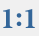
\includegraphics[scale=0.5]{tutorials/figures/1-1.png} button in the top menu.}
            \index{packages!plots}
        \item Solve the equation of the curve for $y$ to get the equations of the top and bottom halves of the ellipse.
        \item Find the $x$-intercepts of this ellipse.
        \item Use the Volume of Revolution Tutor or the \texttt{Int()} command to calculate the area of the solid obtained by revolving the top half of the ellipse about the $x$-axis.
            \index{integral!Int}
    \end{enumerate}
\end{enumerate}
\section{Arc Length and The Golden Gate Bridge Problem}
\label{sec:golden_gate_bridge_problem}	

\subsection*{Recommended Tutorials:}
\begin{itemize}[noitemsep]
    \item \nameref{chp:plotting_functions}, pg. \pageref{chp:plotting_functions}
    \item \nameref{chp:equation_solvers}, pg. \pageref{chp:equation_solvers}
	\item \nameref{chp:definite_and_indefinite_Integrals}, pg. \pageref{chp:definite_and_indefinite_Integrals}
\end{itemize}

\subsection*{Introduction:}
Arc length\index{arc length} is the distance between two points along a section of a curve. If this curve can be represented by a function $f(x)$, then we can calculate the length of this curve from $x=a$ to $x=b$ with the formula
\begin{equation}
    \label{eq:arclength}
    L = \displaystyle\int_{a}^b \sqrt{1 + [f^{\prime}(x)]^2}\, dx.
\end{equation}

In this activity, we will determine the arc length of a variety of functions and curves. We can then apply equation \eqref{eq:arclength} above to determine the length of the cable that holds up the Golden Gate Bridge.

\marginnote[-2cm]{You will have to use the \texttt{sqrt()} command to enter this into Maple.}\index{mathematical functions!square root}

\subsection*{Exercises:}

\begin{enumerate}
    \item Consider the function $y = \cos(\sin(x))$.
    \begin{enumerate}
        \item Plot the graph of the function.
        \item Determine the arc length of this curve between the points $(0,1)$ and $(\pi,1)$.\index{Pi}
    \end{enumerate}
    \marginnote[-0.7cm]{Remember that you must type \texttt{Pi} in Maple for $\pi$.}
    \item Consider the curve $y^2 = x^3$.
    \begin{enumerate}
        \item Plot the graph of the curve using \texttt{implicitplot()}.
            \index{packages!plots}
        \item Solve the equation of the curve for $y$ to get the equations of the top and bottom halves of the curves as functions.
        \item Determine the arc length of this curve between the points $(1,1)$ and $(4,8)$.
    \end{enumerate}
    \item Consider the function $x = \frac{1}{3}\sqrt{y}\,(y-3)$.\marginnote[0.1cm]{Don't forget to include multiplication between $\sqrt{y}$ and $(y-3)$.}
   
    \begin{enumerate} \marginnote[0.2cm]{In this exercise, since $x$ is a function of $y$, equation \eqref{eq:arclength} should be an integral in terms of $y$.}
        \item Plot the graph of the function. Since $x$ is defined as a function of $y$, try plotting the equation of the curve using \texttt{implicitplot()}.
        \item Determine the arc length of this curve for $1 \leq y \leq 9$.
    \end{enumerate}
    \item The main span of the Golden Gate Bridge is $1280$ m long, as shown in Figure \ref{fig:goldengate}. The top of each of the towers is 230 m above the surface of the water. To find the length of the cables between these two towers, we will assume that a freely hanging cable between two towers takes the form of a \textbf{catenary}. 
    \marginnote[-2cm]{A catenary is a curve that an idealized hanging chain or cable assumes under its own weight when supported only at its ends. The Golden Gate Bridge cable is almost a catenary and almost a parabola, but not quite either (because of the weight of the cables, the suspender ropes, and the roadway).}
    \clearpage
    \marginnote[0.5cm]{Functions like $\cosh()$ and $\sinh()$ are called hyperbolic functions. These functions are analogs of the ordinary trigonometric, or circular, functions; just as the points $(\cos(t), \sin(t))$ form a circle with a unit radius, the points $(\cosh(t), \sinh(t))$ form the right half of the equilateral hyperbola.}
        \index{mathematical functions!hyperbolic functions!sinh}
         \index{mathematical functions!hyperbolic functions!cosh}
    The general form for a catenary passing through its lowest point at $(0,k)$ is 
    \begin{equation}
        \label{eq:catenary}
        f(x) = a\left(\cosh\left(\tfrac{x}{a}\right)-1\right)+k,
    \end{equation}
    or equivalently,
    \[f(x) = a\left(\frac{{\rm e}^{x/a} + {\rm e}^{-x/a}}{2}-1\right)+k.\]
	
	\begin{figure*}[h]
        \label{fig:goldengate}
        \centering
    	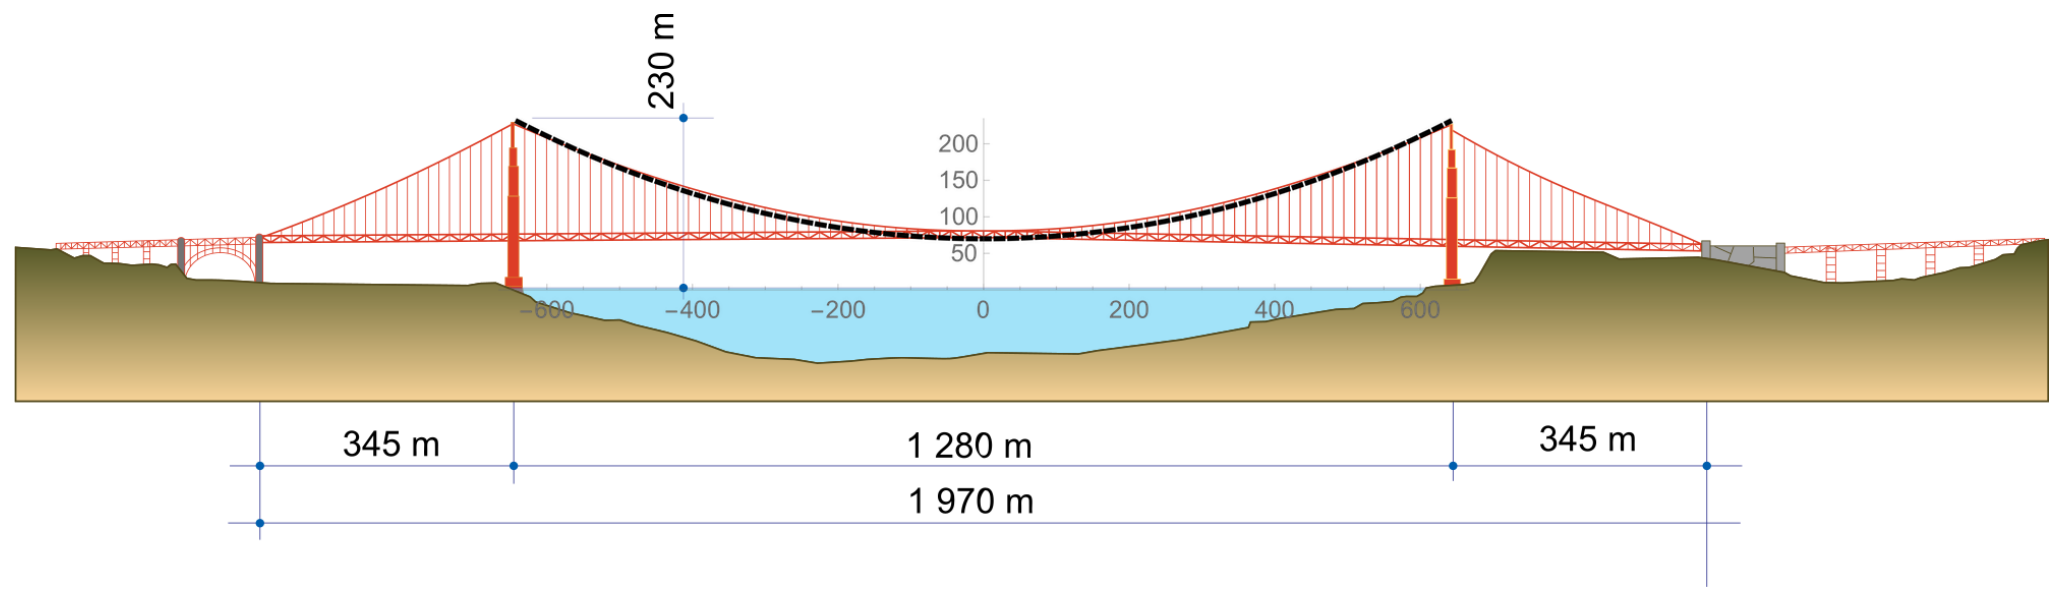
\includegraphics[width=1\linewidth]{activities/math122/figures/goldengate.png}
    	\caption{The portion of the cable for the main span (in black) is approximately the shape of a catenary. The total length of each cable is actually $2{,}332$ m, including the main span and the lengths from both shores.}
    \end{figure*}
    
    Assume that the Golden Gate Bridge cable takes the shape of a catenary over the main span with its lowest point at $(0,70)$, corresponding to a height of $70$ m above the water.
    \begin{enumerate}
        \item Using equation \eqref{eq:catenary} and the points provided in Figure \ref{fig:goldengatesimple}, what is the value of $k$?
        \item Substitute the value of $k$ into \eqref{eq:catenary} and assign this function in Maple.
        \item Use the coordinates of the top of one of the towers from Figure \ref{fig:goldengatesimple}, as well as the \texttt{fsolve()} command to determine the value of $a$ for this catenary.
            \index{solving equations!fsolve}
        \item Using equation \eqref{eq:catenary} with the values of $a$ and $k$ that you have found, determine the length of one of the cables for the main span.
    \end{enumerate}
    
    \begin{marginfigure}[-4cm]
        \hspace{-4cm}
        \centering
        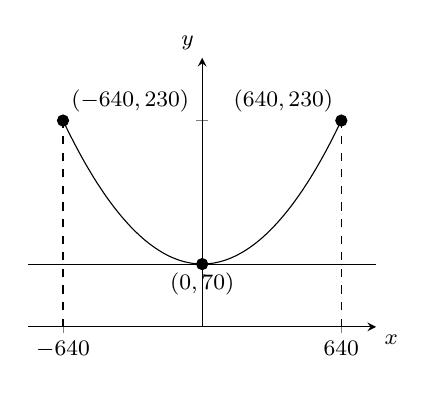
\begin{tikzpicture}
        \footnotesize
        \begin{axis}[
        	width=6cm,
        	height=5cm,
        	axis lines=middle,
        	xlabel={$x$},
        	ylabel={$y$},
        	xlabel style={below right},
        	ylabel style={above left},
        	xmin=-800, xmax=800, xtick={-640,0,640},
        	ymin=0, ymax=300, ytick={0,70,230}, yticklabels={}
        ]
        	\addplot [domain=-640:640, samples=100] {1305.828246*cosh(0.0007657974952*x) - 1235.828246}; %catenary
        	\addplot [domain=-800:800, samples=100] {70}; %bridge deck
        	\addplot[mark=*] coordinates {(-640,230)}; %left tower point
        	\draw(axis cs:-640,230) node [above right] {$(-640,230)$};
        	\addplot[mark=*] coordinates {(640,230)}; %right tower point
        	\draw(axis cs:640,230) node [above left] {$(640,230)$};
        	\addplot[mark=*] coordinates {(0,70)}; %lowest point
        	\draw(axis cs:0,70) node [below] {$(0,70)$};
        	\draw [dashed] (axis cs:-640,0) -- (axis cs:-640,230); %left tower
        	\draw [dashed] (axis cs:640,0) -- (axis cs:640,230); %right tower
        \end{axis}
        \end{tikzpicture}
        \caption{A simplified model of the main bridge span.}
        \label{fig:goldengatesimple}
    \end{marginfigure}
    
    \marginnote[1.5cm]{Interesting fact: The main cables of the Golden Gate Bridge are nearly one meter in diameter (actually, $0.91$ m) and the total length of galvanized steel wire used in both main cables is $129{,}000$ km.}
\end{enumerate}

\section{Infinite Integrals}\index{integral!improper}
\label{sec:infinite_integrals}

\subsection*{Recommended Tutorials:}
\begin{itemize}[noitemsep]
	\item \nameref{chp:plotting_functions}, pg. \pageref{chp:plotting_functions}
	\item \nameref{chp:assignment_operator}, pg. \pageref{chp:assignment_operator}
	\item \nameref{chp:definite_and_indefinite_Integrals}, pg. \pageref{chp:definite_and_indefinite_Integrals}
\end{itemize}

\subsection*{Introduction:}

Infinite integrals are used in a variety of applications, including finding solutions to differential equations by way of the Laplace transform. Infinite integrals can be challenging to evaluate by hand, but in this activity we will see that Maple can handle infinite integrals easily.

\subsection*{Exercises:}

\begin{enumerate}
    \item   
    \begin{enumerate} 
    	\item Define the function $f(x) = \dfrac{1}{\sqrt{2-x}}$ in Maple.
    	\marginnote{Don't forget to use \texttt{sqrt()} when defining this function.}
    	    \index{mathematical functions!square root}
    	\item Plot $f(x)$.
    	    \index{plot!}
    	\item Evaluate the integral $\displaystyle\int_{-\infty}^{-1} f(x) dx$.
    	    \index{integral!}
    \end{enumerate}
    \marginnote[-0.5cm]{It is important to check that the function does not have any points of discontinuity before you integrate.}
    \item   
    \begin{enumerate} 
    	\item Define the function $g(x) = x{\rm e}^{-x^2}$ in Maple.
    	\marginnote{Don't forget to use \texttt{exp()} when defining this function.}
    	\item Plot $g(x)$.
    	\item Evaluate the integral $\displaystyle\int_{-\infty}^{\infty} g(x) dx$.
    \end{enumerate}
    
    \item 
    \begin{enumerate} 
    	\item Define the function $h(x) = \dfrac{\ln x}{x}$ in Maple.
    	\item Plot $h(x)$.
    	\item Evaluate the integral $\displaystyle\int_{1}^{\infty} h(x) dx$.
    \end{enumerate}
    \item   The Laplace transform for a function $J(t)$ is given by the improper integral 
    \[F(s) = \displaystyle\int_{0}^{\infty} J(t){\rm e}^{-st} dt.\]
    \begin{enumerate}
        \item We will assume that $s$ is positive. You will need to type \\
        \texttt{assume(s, positive)} on a new line so that Maple will understand this assumption.
            \index{assume}
        \marginnote{In your output, $s\!\sim$ means that $s$ is now assumed to be a positive value.}
        \item Evaluate the Laplace transform of $J(t) = t$.
    \end{enumerate}
\end{enumerate}

\section{Probability}\index{probability!}
\label{sec:probability}	

\subsection*{Recommended Tutorials:}
\begin{itemize}[noitemsep]
    \item \nameref{chp:assignment_operator}, pg. \pageref{chp:assignment_operator}
	\item \nameref{chp:definite_and_indefinite_Integrals}, pg. \pageref{chp:definite_and_indefinite_Integrals}
\end{itemize}

\subsection*{Introduction:}
In this activity, we define probability density functions (pdf) for some continuous probability distributions. Let’s define our probability function as $f(x)$. If $f(x)$ is a valid probability function, then
\[ \int_{-\infty}^{\infty} f(x)dx=1, \]
and $ 0  \leq f(x) \leq 1$. 
 \index{integral!improper}
 
If we want to compute the probability that a given observation is less than $a$, then we calculate
\[ P(x<a)=\int_{-\infty}^{a} f(x)dx. \]
If we want to compute the probability that the given observation is more than $a$, then we calculate
\[ P(x>a)=\int_{a}^{\infty} f(x)dx. \]
If we want to compute the probability that the given observation is between two values $a$ and $b$, then we calculate 
\[ P(a<x<b)=\int_{a}^{b} f(x)dx. \]

\begin{marginfigure}[-0.5cm]
    \hspace{-4cm}
    \centering
    \begin{tikzpicture}
    \footnotesize
    \begin{axis}[
    width=6cm,
    height=5cm,
    axis lines=middle,
    xlabel={$x$},
    ylabel={$f(x)$},
    xlabel style={below right},
    ylabel style={above left},
    xmin=0, xmax=12, xtick={0,5}, xticklabels={,$\lambda$},
    ymin=0, ymax=0.22, ytick={0,0.2}, yticklabels={,$\frac{1}{\lambda}$}
    ]
        \addplot [domain=0:12, samples=100] {1/5*exp(-1/5*x)};
    \end{axis}
    \end{tikzpicture}
    \caption{The exponential probability density function.}
    \label{fig:exponential_dist}
\end{marginfigure}
    
The exponential distribution is defined as 
\begin{equation}
    \label{eq:exponential_dist}
    f(x) = 
    \begin{cases}
        \lambda{\rm e}^{-\lambda x} & \text{if } x \geq 0 \\
        0 & \text{if } x<0,
    \end{cases}
\end{equation}
    \index{probability!exponential density function}
where $\frac{1}{\lambda}$ is the mean and standard deviation of the probability distribution.

\begin{marginfigure}
    \hspace{-4cm}
    \centering
    \begin{tikzpicture}
    \footnotesize
    \begin{axis}[
    width=6cm,
    height=5cm,
    axis lines=middle,
    xlabel={$x$},
    ylabel={$f(x)$},
    xlabel style={below right},
    ylabel style={above left},
    xmin=0, xmax=12, xtick={0,2,4,6,8,10}, xticklabels={,,,$\mu$,,},
    ymin=0, ymax=0.3, ytick={0,5}, yticklabels={,$\lambda$}
    ]
        \addplot [domain=0:12, samples=100] {1/(2*sqrt(2*pi))*exp(-(x-6)^2/(2*2^2))};
    \end{axis}
    \end{tikzpicture}
    \caption{The normal probability density function.}
    \label{fig:normal_dist}
\end{marginfigure}
    \index{probability!normal probability density function}

Define the normal distribution as 
\begin{equation}
    \label{eq:normal_dist}
    f(x) = \frac{1}{\sigma \sqrt{2\pi}}{\rm e}^{-\frac{(x-\mu)^2}{2\sigma^2}},
\end{equation} 
where $\sigma$ is the standard deviation and $\mu$ is the mean.

\subsection*{Exercises:}

\begin{enumerate}
\item Suppose that the lifetime of a certain tire is exponentially distributed with mean $\frac{1}{\lambda}=45,000$ miles.
\begin{enumerate}
    \marginnote{Examples of the \texttt{piecewise()} command can be found on page \pageref{sec:piecewise}.}
        \index{mathematical functions!piecewise}
	\item Use the \texttt{piecewise()} command to assign the function from equation \eqref{eq:exponential_dist} using $\lambda = \frac{1}{45000}$.
	\item Verify that this function is a valid pdf.
	\marginnote{Hint: take the integral and plot the function to verify this.}
	\item Find the probability that a given tire will last more than $40{,}000$ miles.
	\item Find the probability that a given tire will last less than $50{,}000$ miles.
	\item Find the probability that a given tire will last between $40{,}000$ and $50{,}000$ miles.
	\item Find the probability that a given tire will last exactly $40{,}000$ miles.
\end{enumerate}
\item Suppose that the height of a male is normally distributed with mean $\mu= 178$ cm and standard deviation  $\sigma= 10$ cm.
\begin{enumerate}
    \item Assign the function from equation \eqref{eq:normal_dist} using these values of $\mu$ and $\sigma$.
    \marginnote{The commands \texttt{exp()}, \texttt{sqrt()}, and \texttt{Pi} will all have to be used for this function in Maple.}
    \item Verify that this function is a valid pdf.
        \index{mathematical functions!exponential}
        \index{mathematical functions!square root}
        \index{Pi}
    \item You have a friend who is $7$ ft tall ($213$ cm). Find the probability that a given individual is that height or taller.
    \item Find the probability that a given individual is $213$ cm or smaller.
    \item What is the probability of selecting an individual with a height of exactly $213$ cm?
\end{enumerate}

\end{enumerate}
\section{Motion of a Mass Connected to a Spring}
\label{sec:motion_of_a_mass_connected_to_a_spring}	

\subsection*{Recommended Tutorials:}
\begin{itemize}[noitemsep]
	\item \nameref{chp:differential_equations}, pg. \pageref{chp:differential_equations}
	    \index{differential equations!}
\end{itemize}

\subsection*{Introduction:}
\begin{marginfigure}
    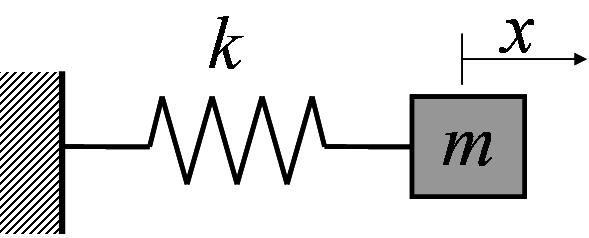
\includegraphics[scale=0.5]{activities/math122/figures/mass_spring.png}
    \caption{A mass on a spring, where $k$ is the spring constant and $x$ measures the displacement of the mass from the equilibrium position ($x=0$).}
    \label{fig:mass_spring}
\end{marginfigure}
According to Hooke's law ($F=-kx$) and Newton's second law ($F=ma$), the differential equation for the motion of a mass ($m$) on the end of a spring is 
\begin{equation*}
m \frac{d^2x}{dt^2}=-kx,
\end{equation*}
    \index{differential equations!hooke's law}
where $k$ is the spring constant (a measure of the stiffness of the spring). This equation assumes no damping (resistance). The displacement of the mass from equilibrium is denoted by $x$, and thus $\frac{dx}{dt}$ is the velocity, and $\frac{d^2x}{dt^2}$ is the acceleration. 

If we add damping (resistance) to the spring, then the damping is opposite the direction of the motion and proportional to the velocity. Therefore we have the equation,
\[ m \frac{d^2x}{dt^2}=-kx-c\frac{dx}{dt}, \]
where $c$ is the damping constant. 

For the exercises, we will assume that the mass is $m=2$-kg and the spring constant is $k=3$ kg/s$^2$. We will look at the equation of motion with no damping ($c=0$), overdamping ($c=4$ kg/s), and underdamping ($c=0.5$ kg/s).

In all cases, we will use the initial conditions $x(0)=1$ m and $x'(0)=-1$ m/s.

\subsection*{Exercises:}

\begin{enumerate}
\item Consider the equation of motion of a $2$-kg mass attached to a spring with $k=3$ kg/s$^2$.
\label{ex:mass_spring_nodamping}
\[ 2 x''(t) = -3 x(t). \]
\begin{enumerate}
    \item Solve the differential equation using the given initial conditions.
    \item Plot the solution of the differential equation.
    \marginnote{The \texttt{rhs()} command may be used to refer to only the right hand side of the differential equation solution. You can use this command to assign a name to the solution.}
    \item Insert a new paragraph and describe what you observe about the motion of a mass on the spring.
        \index{differential equations!rhs()}
\end{enumerate}
\clearpage



\item Consider the equation of motion of a $2$-kg mass attached to a spring with $k=3$ kg/s$^2$ and a damping constant of $c=4$ kg/s. This is considered \textbf{overdamping}.
\[2 x''(t) = -3 x(t) - 4 x'(t).\] \marginnote[-2.5cm]{The solutions to these differential equations will be sine and cosine functions of the form \[\sin(kt) \text{ and } \cos(kt).\] The period $T$ of these oscillations may be found using the formula \[T=\frac{2\pi}{k}.\] }
    \index{mathematical functions!sine}
     \index{mathematical functions!cosine}
     \vspace{-.8cm}
\begin{enumerate}
    \item Solve the differential equation using the given initial conditions.
    \item Plot the solution of the differential equation.
    \item Insert a new paragraph and describe what you observe about the motion of a mass on the spring with overdamping.
\end{enumerate}

\item Consider the equation of motion of a $2$-kg mass attached to a spring with $k=3$ kg/s$^2$ and a damping constant of $c=0.5$~kg/s. This is considered \textbf{underdamping}.
\label{ex:mass_spring_underdamping}
\[ 2 x''(t) = -3 x(t) - 0.5 x'(t). \]
\begin{enumerate}
    \item Solve the differential equation using the given initial conditions.
    \item Plot the solution of the differential equation.
    \item Insert a new paragraph and describe what you observe about the motion of a mass on the spring with underdamping.
\end{enumerate}

\marginnote[-3cm]{To solve these differential equations algebraically you assume that solutions are of the form $x(t)={\rm e}^{rt}$ and then plug it into the differential equation to get the ``characteristic equation" to solve for $r$. If the roots are complex, you will have oscillations (sine and cosine functions) and if the roots are real, then you have strictly exponential solutions. Notice that the overdamped case has no oscillations whereas the underdamping and no-damping cases have oscillations in their solutions.}
     \index{mathematical functions!exponential}

\item Suppose we wish to force the spring to oscillate at a given frequency. Let's add a forcing term $3 \sin(2t)$ to the undamped equation of motion from exercise \ref{ex:mass_spring_nodamping}.
\label{ex:mass_spring_forcing}
\[ 2x''(t) = -3 x(t) + 3\sin(2t) \]
\begin{enumerate}
    \item Solve the differential equation using the given initial conditions.
    \item Plot the differential equation solution.
    \item Insert a new paragraph and describe what you observe about the motion of a mass on the spring with \textbf{forcing and no damping}.
\end{enumerate}

\item Let's add damping to equation of motion from exercise \ref{ex:mass_spring_forcing} with a damping constant of $0.5$ kg/s.
\[ 2x''(t) = -3 x(t) - 0.5 x'(t) + 3\sin(2t) \] 
\begin{enumerate}
    \item Solve the differential equation using the given initial conditions.
    \item Plot the differential equation solution.
    \item Insert a new paragraph and describe what you observe about the motion of a mass on the spring with \textbf{forcing and underdamping}.
\end{enumerate}

\end{enumerate}
\section{Tank Mixing Problem}
\label{sec:tank_mixing_problem}	

\subsection*{Recommended Tutorials:}
\begin{itemize}[noitemsep]
    \item \nameref{chp:equation_solvers}, pg. \pageref{chp:equation_solvers}
    \item \nameref{chp:limits}, pg. \pageref{chp:limits}
        \index{limit!}
	\item \nameref{chp:differential_equations}, pg. \pageref{chp:differential_equations}
	    \index{differential equations!}
\end{itemize}

\subsection*{Introduction:}
\marginnote[-1cm]{Concentration is defined as \[\text{concentration}=\frac{\text{mass}}{\text{volume}}.\] If we wish to determine mass, then we can rearrange the equation to obtain \[\text{mass}=\text{concentration}\times\text{volume}.\]}
Suppose you are having a wedding and you start with a $5$ L tank of coffee that has a concentration of \SI{60}{\gram/\liter}. The wedding guests are drinking the coffee at a rate of \SI{0.2}{\liter/\minute}. You are refilling the tank at a rate of \SI{0.15}{\liter/\minute} with coffee of a concentration of \SI{50}{\gram/\liter}.

\tikzset{
   ragged border/.style={ decoration={random steps, segment length=1mm, amplitude=0.5mm},
           decorate,
   }
}
\begin{figure}[h]
\begin{tikzpicture}
    \fill[cyan!30]
    decorate[ragged border]{
        (0,2) -- (6,2)
    }
    -- (6,1) -- (6.5,1) -- (6.5,0.5) -- (6,0.5) --(6,0) -- (0,0) -- cycle;
    \fill[cyan!30] (-0.5,2.5) -- (0,2.5) to[in=120,out=0](0.7,1.9)-- (1.4,1.9)
                  to[out=120,in=0] (0,3) -- (-0.5,3) -- cycle;
    \draw (-0.5,2.5) -- (0,2.5) -- (0,0) -- (6,0) -- (6,0.5) -- (6.5,0.5);
    \draw (-0.5,3) -- (0,3) -- (0,3.5) -- (6,3.5) -- (6,1) -- (6.5,1);
    \draw[|-|] (-0.3,0) --
        node[fill=white,font=\footnotesize,inner ysep=2pt,inner
                xsep=0]{$V(t)$}(-0.3,2);
    \draw[stealth-] (-0.5,2.75) -- (-1,2.75)
            node[anchor=east,font=\footnotesize,align=right]{\SI{0.15}{\liter/\minute}\\\SI{50}{\gram/\liter}};
    \draw[-stealth] (6.5,0.75) -- (7.2,0.75)
            node[anchor=west,font=\footnotesize]{\SI{0.2}{\liter/\minute}};
    \node[anchor=north,font=\footnotesize] at (3,3.5) {
        $\begin{array}{l}
             V(t)=? \\
             m(t)=? \\
             C(t)=?
        \end{array}$
    };
    \node[anchor=north,font=\footnotesize] at (3,1.5) {
        $\begin{array}{l}
             V(0)=\SI{5}{\liter}  \\
             m(0)=\SI{300}{\gram} \\
             C(0)=\SI{60}{\gram/\liter}
        \end{array}$
    };
\end{tikzpicture}
\caption{An illustration of the tank of coffee. The initial conditions for the volume and mass of coffee are shown.}
\label{fig:coffe_tank}
\end{figure}
\vspace{-1.4cm}

\subsection*{Exercises:}

\begin{enumerate}
\item 
\begin{enumerate}
    \item Setup a differential equation for the volume of coffee in the tank using $V'(t) = (\text{rate in}) - (\text{rate out}).$
    \item Solve this differential equation using the initial condition to obtain a formula for the volume $V(t)$ after $t$ minutes.
    \item Use the \texttt{solve()}\index{solving equations!solve} command to compute how long it will be until you run out of coffee.
\end{enumerate}
\item 
\begin{enumerate}
    \item Set up a differential equation for the mass of coffee in the tank using 
    \[m'(t) = \lrp{\begin{array}{l}
         \text{concentration}  \\
         \text{entering tank} 
    \end{array}}
    \lrp{\begin{array}{l}
         \text{volume}  \\
         \text{rate in} 
    \end{array}}
    -
    \lrp{\begin{array}{l}
         \text{concentration}  \\
         \text{in tank at time }t 
    \end{array}}
    \lrp{\begin{array}{l}
         \text{volume}  \\
         \text{rate out} 
    \end{array}}.\]
    \item Solve the differential equation for mass using your initial condition for the mass of the coffee $m(t)$ after $t$ minutes.
\end{enumerate}
\item Determine the function for the concentration of the coffee in the tank $C(t)$ after $t$ minutes using $C(t) = m(t)/V(t)$.
\item Plot $V(t)$, $m(t)$, and $C(t)$ on separate graphs to see what happens to the mass, volume, and concentration over time.
\item Use the \texttt{limit()}\index{limit} command to determine the concentration of coffee as you approach the last drop of coffee.
\end{enumerate}	
\section{Direction Fields}
\label{sec:direction_fields}	

\subsection*{Recommended Tutorials:}
\begin{itemize}[noitemsep]
	\item \nameref{chp:differential_equations}, pg. \pageref{chp:differential_equations}
	    \index{differential equations}
\end{itemize}

\subsection*{Introduction:}
In this activity, you will use direction fields to predict the population dynamics for a population of rabbits. Suppose that you have a population of rabbits and $P(t)$ is the number of rabbits at time $t$. 

\marginnote{You will need to include the \texttt{DETools} package to use the \texttt{DEplot()} command.}
    \index{differential equations!DETools}
    \index{packages!differential equations!DETools!DEplot()}

We can model the population of rabbits using a basic model
\begin{equation}
\label{eq:rabbits_basic}
\frac{dP}{dt}=\alpha P - \beta P,
\end{equation}
where $\alpha$ is the birth rate and $\beta$ is the death rate.

Equation \eqref{eq:rabbits_basic} does not consider limitations due to habitat and food supply. If we wish to use a more accurate model, then we can consider the logistic growth model
\begin{equation}
\label{eq:rabbits_logistic}
\frac{dP}{dt}= kP \left(1-\frac{P}{M}\right),
\end{equation}
where $k$ is the relative growth rate and $M$ is the carrying capacity (the maximum population that is sustainable). 

The death rate of the rabbits (due to hunting) can be added to this logistic model to obtain the differential equation
\begin{equation}
\label{eq:rabbits_logistic_hunted}
\frac{dP}{dt}=kP \left(1-\frac{P}{M}\right)-bP,
\end{equation}
where $b$ is the hunting rate. 

We will examine solutions to equations \eqref{eq:rabbits_basic}--\eqref{eq:rabbits_logistic_hunted} using two different initial conditions: $P(0)=1$ and $P(0)=50$.

\subsection*{Exercises:}

\marginnote[0.5cm]{Remember to use $P(t)$ and not just $P$ in your differential equation.}
\begin{enumerate}
\item Consider the basic population model in equation \eqref{eq:rabbits_basic}.
\begin{enumerate}
    \item Draw the direction field using $\alpha=2$ and $\beta=1$, including both initial conditions given.
    \item Draw the direction field using $\alpha=1$ and $\beta=2$, including both initial conditions given.
    \item In a new paragraph in your worksheet, describe what you can conclude about the importance of the death to birth rate comparison.
\end{enumerate}
\clearpage
\item Consider the logistic growth model in equation \eqref{eq:rabbits_logistic}.
\label{ex:rabbits_logistic}
\begin{enumerate}
    \item Draw the direction field using $k=2$ and $M=30$, including both of the initial conditions given.
        \index{differential equations!DEplot}
    \item In a new paragraph, describe what you observe about the solutions.
\end{enumerate}
\item Consider the logistic growth model in equation \eqref{eq:rabbits_logistic_hunted}.
\begin{enumerate}
    \item Draw the direction field using $k=2$, $M=30$, and $b=1$, including both of the initial conditions given.
    \item In a new paragraph in your worksheet, describe what changed from exercise \ref{ex:rabbits_logistic} by adding the death rate to the differential equation.
\end{enumerate} 
\end{enumerate}

Most mammal population growth is dependent upon other species in the region, via an interconnected food web. One simple predator-prey model is the Lotka-Volterra model
\begin{align}
\label{eq:rabbits_lotka_volterra}
\frac{dx}{dt} &= \alpha x-\beta xy\\
\frac{dy}{dt} &= \gamma xy-\delta y,\nonumber
\end{align}
\marginnote[-1.25cm]{Make sure you insert multiplication between $x(t)$ and $y(t)$ here, otherwise Maple will think you want to use a variable called $xy$.}
where $x(t)$ is the population of prey and $y(t)$ is the population of predators. In this equation, the prey grow and are eaten by predators. The predators' growth depends on eating the prey and the predators have a death rate.

\begin{enumerate}
\setcounter{enumi}{3}
\item Consider the Lotka-Volterra model in equation \eqref{eq:rabbits_lotka_volterra}.
\begin{enumerate}
    \item Go to Tools, Tutors, Differential Equations, DE Plots, select Lotka-Volterra Model, and then DEPlot. If you want, you can change the parameters or the initial conditions. Then click quit to plot it on your Maple worksheet. 
    \item In a new paragraph, explain what the prey and predator populations do on this direction field. Notice that the prey is on the $x$-axis and the predator is on the $y$-axis of the direction field.
    \index{differential equations!DETools}
    \index{packages!differential equations!DETools!DEplot()}
\end{enumerate}
\end{enumerate}

\section{Series Convergence and Divergence}
\label{sec:series_convergence_and_divergence}	

\subsection*{Recommended Tutorials:}
\begin{itemize}[noitemsep]
    \item \nameref{chp:definite_and_indefinite_Integrals}, pg. \pageref{chp:definite_and_indefinite_Integrals}
        \index{integral}
        \index{integral!improper}
	\item \nameref{chp:sequence_and_sseries}, pg. \pageref{chp:sequence_and_sseries}
	    \index{sequences and series!}
\end{itemize}

\subsection*{Introduction:}

An infinite series is a summation of the form
\[ \sum_{n=0}^{\infty} a_n = a_0 + a_1 + a_2 + \dots. \]
For example, we can look at the geometric series
\begin{equation}
    \label{eq:geometric_series}
    \sum_{n=0}^{\infty} \frac{1}{2^n} = 1 + \frac{1}{2} + \frac{1}{4} + \frac{1}{8} + \dots.
\end{equation}
To understand the result of the sum in equation \eqref{eq:geometric_series}, we can add the first few terms, one at a time. 
\begin{align*}
    1+\frac{1}{2} &= \frac{3}{2}\\
    1+\frac{1}{2}+\frac{1}{4} &= \frac{7}{4}\\
    1+\frac{1}{2}+\frac{1}{4}+\frac{1}{8} &= \frac{15}{8}\\
\end{align*}
By looking at these partial sums, we can see that the sum is approaching the value $2$. We say that this series is \textit{convergent}. In other cases, the partial sums do not approach a finite value. We say that these series are \textit{divergent.}
    \index{sequences and series!divergent}
    \index{sequences and series!convergent}

In this activity, we will use Maple to evaluate whether a series is convergent or divergent. Maple will give the value of the sum for a convergent series and will give the value $\infty$ or $-\infty$ if the series is divergent.\index{infinity}

\subsection*{Exercises:}

\begin{enumerate}
\item For each of the following series, set up the series symbolically using the \texttt{Sum()} command. Then, use the \texttt{value(\%)} command to evaluate the sum and determine if it converges.
    \index{sequences and series!Sum}
    \index{value}
    \index{ditto operator}
\marginnote[0.5cm]{For (b), make sure you use "\texttt{Pi}" for $\pi$ and place multiplication between the $n$ and \texttt{Pi}.}
    \index{Pi}
\begin{multicols}{2}
\begin{enumerate}
    \item $\displaystyle\sum_{n=0}^{\infty} \dfrac{4^n}{n!}$
    \item $\displaystyle\sum_{n=0}^{\infty} \sin(n\pi)\arctan(n)$
    \item $\displaystyle\sum_{n=1}^{\infty} \ln(n)$
    \item $\displaystyle\sum_{n=1}^{\infty} \dfrac{n!}{n^2}$
\end{enumerate}
\end{multicols}
\end{enumerate}
\clearpage
The Integral Test for Convergence states that for a non-negative, monotonically decreasing function $f(n)$ and an integer $N$, the infinite series $$\sum_{n=N}^{\infty} f(n)$$ converges to a real number if and only if the improper integral $$\int_N^{\infty} f(x)\,dx$$ is finite. From this, we can also conclude that if the integral diverges, then the series diverges as well.\\
\begin{enumerate}
\setcounter{enumi}{1}
\item Consider the series
\[ \sum_{n=3}^{\infty}\dfrac{3}{n^2-3n+2}. \]
\begin{enumerate}
    
    \item Graph the function $f(x) = \dfrac{3}{x^2-3x+2}$ to see that the function is non-negative and monotonically decreasing over the interval $[3,\infty)$.
    \marginnote[-1.5cm]{After plotting $f(x)$, try to think about why this series starts at $n=3$.}
    \item Use the Integral Test to determine whether or not the series converges or diverges.
\end{enumerate}
\end{enumerate}
\section{Taylor and Maclaurin Series}
\label{sec:taylor_series}	

\subsection*{Recommended Tutorials:}
\begin{itemize}[noitemsep]
	\item \nameref{chp:sequence_and_sseries}, pg. \pageref{chp:sequence_and_sseries}  
	    \index{sequences and series}
\end{itemize}

\subsection*{Introduction:}
The Taylor series of a function $f$ centred at $a$ is given by the equation
    \index{sequences and series!Taylor and Maclaurin series}
\begin{align*}
f(x) 
&= \sum_{n=0}^{\infty} \frac{f^{(n)}(a)}{n!}(x-a)^n\\
&= f(a) + \frac{f'(a)}{1!}(x-a) + \frac{f''(a)}{2!}(x-a)^2 + \frac{f'''(a)}{3!}(x-a)^3 + \cdots.
\end{align*}
The Maclaurin series is a special case of the Taylor series, where $a=0$:
    \index{sequences and series!Taylor and Maclaurin series!formula}
\[
f(x) 
= \sum_{n=0}^{\infty} \frac{f^{(n)}(0)}{n!}x^n 
= f(0) + \frac{f'(0)}{1!}x + \frac{f''(0)}{2!}x^2 + \frac{f'''(0)}{3!}x^3 + \cdots.
\]

In both series, we can use partial sums to approximate the shape of the function $f(x)$ in a region centred at $a$ by a polynomial. In this activity, we will compute and plot Taylor and Maclaurin series approximations to understand how the radius of convergence works.
\marginnote[-0.5cm]{The radius of convergence for a Taylor series is the values of $x$ for which a Taylor series will converge to the function $f(x)$.}

\subsection*{Exercises:}

\begin{enumerate}
\item Consider the function $f(x) = \cos(x)$.
	\begin{enumerate}
	\marginnote{Examples of finding and plotting Taylor series can be found on page \pageref{sec:taylor_and_maclaurin_series}.}
	\item Compute the Maclaurin series of $f(x)$ accurate to order $3$ using \\
	\texttt{taylor(cos(x), x=0, 3)}. Convert this to a polynomial and assign it to \textit{poly3} using the command \\
	\texttt{poly3 := convert(\%, polynom)}.
	    \index{sequences and series!Taylor and Maclaurin series!taylor}
	    \index{sequences and series!Taylor and Maclaurin series!convert to polynomial}
	    \index{ditto operator}
	\item Repeat part (a) using orders $6$, $12$, and $24$. Assign each of these polynomials to a different name.
    \marginnote[0.5cm]{You may want to choose different colours for each of these four curves to keep track of which is which if you plan to plot all of them on the same set of axes.} 
    \item Plot the graph of $f(x)$ and the Maclaurin series from parts (a) and (b).
        \index{plot}
    \item In a new paragraph, describe what happens to the graph of the Maclaurin series approximation as we increase its order (that is, have higher degree polynomials).
    \item If we increase our order to infinity, we expect that the approximation will converge to the radius of convergence on either side of $0$. In a new paragraph in your worksheet, state what you expect the radius of convergence to be.
	\end{enumerate}
	\clearpage
\item Consider the function $g(x) = \ln(1+x)$.
	\begin{enumerate}
	\item Find the Maclaurin series of $g(x)$.
    \item Compute the Maclaurin series of $g(x)$ accurate to orders $3$, $6$, $12$, and $24$. 
    \item Plot the graph of $g(x)$ and the Maclaurin series from part (b).
    \marginnote[-0.5cm]{You may want to choose different colours for each curve to keep track of which is which.} 
    \item In a new paragraph in your worksheet, state what you expect the radius of convergence to be.
	\end{enumerate}
	
\item It turns out that the full Taylor series for the functions from exercises $1$ and $2$ are
\begin{align*}
\cos(x)&=\sum_{n=0}^{\infty} \frac{(-1)^n x^{2n}}{(2n)!} \\
\ln(1+x)&=\sum_{n=0}^{\infty} \frac{(-1)^{n-1} x^n}{n}
\end{align*}

Find the radius of convergence for these two series by hand in the space below. In a new paragraph, confirm whether or not it matches your predictions from your Maple plots.

\begin{fullwidth}
    \fbox{\parbox{1\linewidth}{$\displaystyle\cos(x)=\sum_{n=0}^{\infty} \frac{(-1)^n x^{2n}}{(2n)!}$ \vspace{5cm} }}
    \fbox{\parbox{1\linewidth}{$\displaystyle\ln(1+x)=\sum_{n=0}^{\infty} \frac{(-1)^{n-1} x^n}{n}$ \vspace{5cm} }}
\end{fullwidth}

\end{enumerate}
%\section{Approximations of $\pi$}
\label{sec:approximations_of_pi}		

\subsection*{Recommended Tutorials:}
\begin{itemize}[noitemsep]
	\item \nameref{chp:sequence_and_sseries}, pg. \pageref{chp:sequence_and_sseries}
\end{itemize}
\subsection*{Introduction:}

In this activity, we will see how Taylor series can be used in order to approximate $\pi$.

We know that the Taylor series of $\arctan(x)$ centred at $0$ is
\[\arctan(x) = \sum_{n=0}^{\infty} \dfrac{(-1)^n x^{2n+1}}{2n+1}.\]
From this, we can use the $k$\textsuperscript{th} partial sum 
\begin{equation}
    \label{eq:arctan_partial_sum}
    \sum_{n=0}^{k} \dfrac{(-1)^n x^{2n+1}}{2n+1}
\end{equation}
to approximate $\pi$ to as many digits as necessary. How quickly can we determine the value of $\pi$ accurate to $15$ digits using equation \eqref{eq:arctan_partial_sum}?
\marginnote[-1.5cm]{Borwein, Bailey, and Plouffe published a formula for $\pi$ that allows someone to find the $n^{th}$ binary digit of $\pi$ without needing to find any preceding digit.  Their formula, 
\begin{align*}
\scriptsize \pi = \displaystyle\sum_{k=0}^{\infty} &\left[\dfrac{1}{16^k}\left(\dfrac{4}{8k+1} - \dfrac{2}{8k+4}\right.\right.\\
		&\left.\left. - \dfrac{1}{8k+5} - \dfrac{1}{8k+6}\right)\right],
\end{align*}
\noindent was published in the paper ``On the Rapid Computation of Various Polylogarithmic Constants'' in which they compute the $10$ billionth hexadecimal digit of $\pi$.  Can you see how this formula lends itself well for this type of calculation?}

\subsection*{Exercises:}

\begin{enumerate}
    \item   As $k \rightarrow \infty$, we know that $\arctan(1) = \pi/4$.  How large does $k$ need to be in order to approximate $\pi$ accurate to $15$ digits?
    \item   As $k \rightarrow \infty$, we know that $\arctan(1/2) + \arctan(1/3) = \pi/4$.  How large does $k$ need to be in order to approximate $\pi$ accurate to $15$ digits?
    \item   As $k \rightarrow \infty$, we know that $2\arctan(1/2) - \arctan(1/7) = \pi/4$.  How large does $k$ need to be in order to approximate $\pi$ accurate to $15$ digits?
    \item   As $k \rightarrow \infty$, we know that $2\arctan(1/3) + \arctan(1/7) = \pi/4$.  How large does $k$ need to be in order to approximate $\pi$ accurate to $15$ digits?
    \marginnote[-1cm]{Many other formulas exist that can be used to approximate $\pi$ including $\dfrac{\pi}{4} = 5\arctan(1/7) + 2\arctan(3/79)$.}
    \item   As $k \rightarrow \infty$, we know that $4\arctan(1/5) - \arctan(1/239) = \pi/4$.  How large does $k$ need to be in order to approximate $\pi$ accurate to $15$ digits?
    \marginnote[-1cm]{The only possible formulas with two terms using $\arctan(1/k)$ to approximate $\pi/4$ are the ones listed in the exercises in this activity (Borwein and Bailey $2003$).}
    \item   As $k \rightarrow \infty$, we know that $\arctan(1/2) + \arctan(1/5) + \arctan(1/8) = \pi/4$.  How large does $k$ need to be in order to approximate $\pi$ accurate to $15$ digits?
    \marginnote[-0.5cm]{It is important to understand why some of these series converge quicker than others.}
    \item   On a separate sheet of paper, use the power series for $\arctan(x)$ to prove that \\
    \[\pi = 2\sqrt{3} \displaystyle\sum_{n=0}^{\infty} \dfrac{(-1)^n}{(2n+1)3^n}.\]  It may help to recall that $\arctan(1/\sqrt{3}) = \pi/6$.
\end{enumerate}


\chapter{Lab Test Review for Math 122}

The following exercises are provided as examples of potential questions on the final lab test at the end of the semester.

\begin{enumerate}

\section*{Riemann Sums}\index{integral approximation!Riemann sum}

\item Assign the function $f(x) = x \lrp{1-x^2 {\rm e}^{-\frac{1}{6}x^2}}$ in Maple.
	\begin{enumerate}
	\item Evaluate the Riemann sum over the interval $\lrb{-4,2}$ using the \texttt{method=lower} option with $8$ partitions.
	\item Evaluate the Riemann sum over the interval $\lrb{-4,2}$ using the \texttt{method=upper} option with $8$ partitions.
	\end{enumerate}
	
\section*{Integral Approximation Techniques}
    \index{integral approximation!ApproximateInt}

\item Assign the following function in Maple: \[ g(x) = \sqrt{x} \sin(x) \]
	\begin{enumerate}
	\item Give an approximate value of $\dint_{1}^{8} g(x)~dx$ using the midpoint rule and $10$ partitions.
	\item Give an approximate value of $\dint_{1}^{8} g(x)~dx$ using the trapezoid rule and $10$ partitions.
	\item Give an approximate value of $\dint_{1}^{8} g(x)~dx$ using Simpson's rule and $10$ partitions.
	\item Give the exact value of the definite integral $\dint_{1}^{8} g(x)~dx$ and evaluate as a decimal with $15$ digits.
	\end{enumerate}

\section*{Integral Functions and the Fundamental Theorem of Calculus}\index{integral}

\item Consider the function \[ f(x) = \dint_{0}^{x} 10 {\rm e}^{-0.5 t} \sin(t) \: dt. \]
	\begin{enumerate}
	\item Assign the function to $f(x)$ and plot it over the interval $[0,10]$.
	\item What is the derivative, $f'(x)$?
	\item At what value in the interval $[0,10]$ does $f(x)$ reach its maximum?
	\item What is the maximum value of $f(x)$ over the interval $[0,10]$?
	\end{enumerate}

\section*{Areas Between Curves}\index{integral!net area}\index{integral!total area}

\item Assign the following function in Maple: $$h(x) = \dfrac{2x}{x^2+6}$$
	\begin{enumerate}
	\item Find the \textbf{net} area bounded by $h(x)$ and the $x$--axis on the interval $\lrb{-2,6}$.
	\item Find the \textbf{total} area bounded by $h(x)$ and the $x$--axis on the interval $\lrb{-2,6}$.
	\end{enumerate}

\item Plot the region between the curves $f(x) = \tan^2(x)$ and $g(x) = \sqrt{x}$ and compute the area to $15$ digits.

\section*{Average Value of a Function}\index{average value of a function}

\item Find the average value of $f(x) = 2\sin(x) - \sin(2x)$ on the interval $[0,\pi]$.
	
\section*{Volumes of Revolution}\index{volume of revolution}

\item Find the volume of the egg-shaped solid obtained by revolving the region bounded by the implicit curve \[ 4x^2 + y^2 = 12 \] about the $x$-axis.

\item Find the volume bounded by the curves $y^2 - x^2 = 1$ and $y=2$ rotated about the $x$-axis.

\section*{Arc Length}\index{arc length}

\item Determine the arc length of the curve $f(x) = x\sqrt[3]{4-x}$ over the interval $[0,4]$ to $15$ digits.

\section*{Infinite Integrals and Probability}
    \index{integral!improper}
    \index{probability}

\item At an annual triathlon, the finishing times for male athletes can be modeled by the probability density function
\[ p(x) = \dfrac{1}{\sigma \sqrt{2\pi}} {\rm e}^{-(x-\mu)^2/2\sigma^2}, \]
where $\mu = 4313$ seconds (the average finish time) and $\sigma = 583$ seconds (the standard deviation of finish times). Define this function in Maple using the specified values of $\mu$ and $\sigma$.
	\begin{enumerate}
	\item Plot the function over the interval $[0,6500].$
	\item What is the probability that a male athlete finishes the triathlon in under $3600$ seconds ($1$ hour)?
	\item What is the probability that a male athlete finishes the triathlon in over $4200$ seconds ($1$ hour $10$ min)?
	\item What is the probability that a male athlete takes between $3600$ and $5400$ seconds to finish the triathlon ($1$ hour to $1.5$ hours)?
	\end{enumerate}
	
\section*{Differential Equations}
    \index{differential equations}

\item After $500$ fish are introduced to a lake, the rate of growth for the population of fish is given by the differential equation
\[ \frac{dN}{dt} = \dfrac{N\lrp{7000 - N}}{10000}, \]
where $N=N(t)$ is the population of fish after $t$ years. Define this differential equation in Maple.
	\begin{enumerate}
	\item Use \texttt{dsolve()} to give the solution to the differential equation for $N(t)$ using the initial condition $N(0)=500$.
	\item How many fish will there be after $6$ years (to the nearest fish)?
	\item What does the population of fish approach after a long time? (Take the limit as $t$ tends to infinity or use a plot).
	\end{enumerate}

\section*{Taylor Series}
    \index{sequences and series!Taylor and Maclaurin series}

\item Find the Taylor series expansion of $f(x) = {\rm e}^{2x} \tan(x)$ centred at $x=0$ (Maclaurin series) and give the coefficient of the $x^8$ term.

\end{enumerate}

\clearpage

\section*{Solutions}

\begin{enumerate}
    \item (a) $1.06499989996052$ \\(b) $7.98649893432598$
    \item (a) $0.87353651353133$ \\(b) $0.799055557908822$ \\(c) $0.848709528323826$ \\(d) $0.848559602278512$
    \item (b) $10 {\mathrm e}^{- 0.5 x} \sin\! \left(x\right)$ \\(c) $3.14159265358979$ \\(d) $9.66303661080610$
    \item (a) $1.43508452528932$ \\(b) $2.45673577282130$
    \item $0.251416829858820$
    \item $1.27323954473516$
    \item $87.0623694832426$
    \item $21.7655923708106$
    \item $7.79878582727266$
    \item (b) $0.110667763524550$ \\(c) $0.576843561268247$ \\(d) $0.858206054544922$
    \item (a) $N\! \left(t\right)=\frac{7000}{1+13 {\mathrm e}^{-7 t/10}}$ \\(b) $5858.02246368622$ \\(c) $7000$
    \item $2/5$
\end{enumerate}

%----------------------------------------------------------------------------------------------

\part{Tutorials}
\label{pt:Tutorials}

\setcounter{chapter}{0}
\renewcommand{\thechapter}{\Alph{chapter}}
\renewcommand{\theHchapter}{otherchapter\thechapter}

\chapter{The Maple Environment}
\label{chp:maple_environment}			

\section{Execution Groups}
\label{sec:execution_groups}

Maple input is used for computations and must use recognizable commands. Maple output gives the result of the computation after hitting the Enter key. Together, Maple input and output are called an \textit{execution group}.
\begin{itemize}
\item Place a new execution group after the current line with the 
\includegraphics[width=0.05\textwidth]{tutorials/figures/new_input.PNG} button.
\item Place a new execution group after the current line with Ctrl+J.
\item Place a new execution group before the current line with Ctrl+K.
\end{itemize}
Maple input is preceded by the $>$ character (sometimes called a "carrot"). Maple output is displayed in the centre of the following line.

\begin{marginfigure}
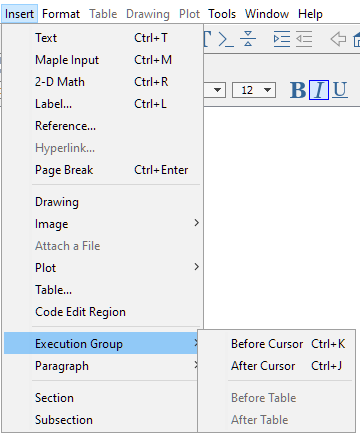
\includegraphics[scale=0.5]{tutorials/figures/InsertInput.png}
\caption{Using the Insert menu to include a new Maple execution group.}
\end{marginfigure}

\begin{maplegroup}
\begin{mapleinput}
\mapleinline{active}{1d}{2 + 2;
}{}
\end{mapleinput}
\mapleresult
\begin{maplelatex}
\mapleinline{inert}{2d}{4}{\[\displaystyle 4\]}
\end{maplelatex}
\end{maplegroup}
\begin{maplegroup}
\begin{mapleinput}
\mapleinline{active}{1d}{8 / 2;
}{}
\end{mapleinput}
\mapleresult
\begin{maplelatex}
\mapleinline{inert}{2d}{4}{\[\displaystyle 4\]}
\end{maplelatex}
\end{maplegroup}

If at any point you wish to correct a previous Maple input line, you may simply go back to that line and modify it. However, there will be no change to the output until you hit Enter. You do not need to be at the end of the line in order to run it.

You may wish to have more than one calculation or command on a single Maple input. For more information on this, see Tutorial \ref{chp:basics_of_maple_syntax} on page \pageref{chp:basics_of_maple_syntax}.

\section{Paragraphs}
\label{sec:paragraphs}

\begin{marginfigure}
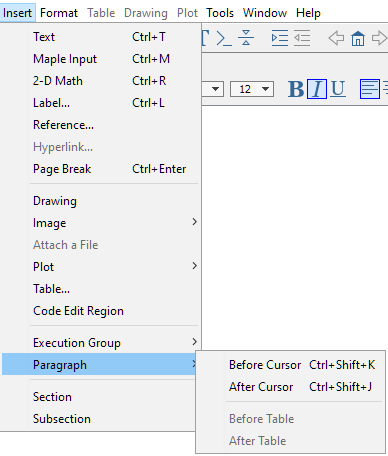
\includegraphics[scale=0.5]{tutorials/figures/InsertParagraph.png}
\caption{Using the Insert menu to include a new text paragraph.}
\end{marginfigure}

\textit{Paragraphs} are used for text, rather than for computation. Hitting Enter simply creates a new line of text and does not try to display a result.
\begin{itemize}
\item Create new text after the current line with the 
\includegraphics[width=0.04\textwidth]{tutorials/figures/new_text.PNG} button.
\item Create new text after the current line with Ctrl+Shift+J.
\item Create new text before the current line with Ctrl+Shift+K.
\end{itemize}

\section{Deleting Inputs}
\label{sec:deleting_intputs}

\marginnote{It's a good habit to delete unnecessary Maple inputs.}
Delete a section of Maple Input or Text using Ctrl+Delete. You will notice that hitting backspace will not delete a section by default.

\section{Three Font Styles}
\label{sec:three_font_styles}

There are two font styles that are commonly used in execution groups.
\begin{itemize}
\item ``2D Math" (the default in modern versions)
	\begin{itemize}
	\item In this mode, mathematical expressions are formatted nicely, as one would write them on paper. 
	\item Text will appear in \textit{italic}, with the exception of common mathematical functions and constants.
	\item An example of an expression in 2D Math: \[\displaystyle {\frac {{x}^{5}}{{\rm e}^{x}+\sin \left( x \right) }}. \]
	\item Switch to 2D Math using Ctrl+R.
	\end{itemize}
	\marginnote[-2cm]{While 2D Math has the advantage of looking prettier, it often treats spaces as multiplication and it doesn't always treat brackets as multiplication when desired. Maple Input causes fewer issues with how Maple interprets what has been typed, but it often requires the use of many more parenthesis. This lab manual will make frequent use of Maple Input for clarity, but you will likely use 2D Math for most of your exercises.}
\item ``Maple Input" (the default for old versions)
	\begin{itemize}
	\item In this mode, mathematical expressions are displayed inline, with no additional formatting. 
	\item All text is shown in \texttt{monospaced font}.
	\item The above expression in Maple input: 
		\begin{verbatim}
		x^5/(exp(x)+sin(x))
		\end{verbatim}
	\item Switch to Maple Input using Ctrl+M.
	\end{itemize}
\end{itemize}
Finally, paragraphs use a third style of font.
\begin{itemize}
\item ``Plain Text"
\marginnote{It can be useful to switch to 2D Math in paragraphs for an expression or equation, then switch back to text afterwards.}
	\begin{itemize}
	\item In this mode, mathematical expressions are displayed inline, with no additional formatting. 
	\item All text is shown in a standard font, such as this line.
	\item Switch to Plain Text using Ctrl+T.
	\end{itemize}
\end{itemize}

\section{Using Sections}
\label{sec:using_sections}

\textit{Sections} are groups of one or more execution groups or paragraphs that are indented together. At the top of a section, you can create a section title. An arrow to the left of the title will allow you to expand or collapse that section. Subsections may be created inside other sections.

\begin{itemize}
\marginnote{You may wish to highlight several execution groups or paragraphs with the mouse before combining them into one section.}
\item Use the 
\includegraphics[width=0.1\textwidth]{tutorials/figures/new_section.PNG} buttons to create or remove sections.
\item Use Ctrl+. to enclose input in a section.
\item Use Ctrl+, to remove any section enclosing an input.
\end{itemize}

\section{Palettes Toolbar}
\label{sec:palettes_toolbar}

You can open or close the palettes toolbar by clicking on the black arrows at the left side of the page.
\begin{figure}
\adjincludegraphics[width=0.495\textwidth]{tutorials/figures/palettes1.png}\hspace{.2cm}
\adjincludegraphics[width=0.505\textwidth]{tutorials/figures/palettes2.png}
\caption{Opening and closing the palettes toolbar.}
\end{figure}

With the palettes toolbar open, you can see several palettes that are available. These can be used to quickly access common operations and procedures by clicking on the appropriate buttons. Each palette can be expanded or closed. The Expression palette is especially useful for common functions.

\begin{marginfigure}
\centering
\adjincludegraphics[scale=0.6,trim={0 {.3\height} 0 0},clip]{tutorials/figures/palettes3.png}
\caption{The first few default palettes expanded.}
\end{marginfigure}

\chapter{Basics of Maple Syntax}
\label{chp:basics_of_maple_syntax}

\section{Algebraic Operations}

At its elementary level, Maple can be used as a really large, powerful calculator. It can do any arithmetic operation including, but not limited to, addition (+), subtraction (-), multiplication (*), division (/), powers (\textasciicircum), and other more complicated operations such as radicals (roots), logarithms, and exponentials. Anytime Maple performs an arithmetic operation, it is creating an \textit{expression}.

\begin{maplegroup}
\begin{mapleinput}
\mapleinline{active}{1d}{a + b;
}{}
\end{mapleinput}
\mapleresult
\begin{maplelatex}
\mapleinline{inert}{2d}{a+b}{\[\displaystyle a+b\]}
\end{maplelatex}
\end{maplegroup}

\begin{maplegroup}
\begin{mapleinput}
\mapleinline{active}{1d}{a - b;
}{}
\end{mapleinput}
\mapleresult
\begin{maplelatex}
\mapleinline{inert}{2d}{a-b}{\[\displaystyle a-b\]}
\end{maplelatex}
\end{maplegroup}

\begin{maplegroup}
\begin{mapleinput}
\mapleinline{active}{1d}{a * b;
}{}
\end{mapleinput}
\mapleresult
\begin{maplelatex}
\mapleinline{inert}{2d}{a*b}{\[\displaystyle ab\]}
\end{maplelatex}
\end{maplegroup}

\marginnote{In 2D Math mode (the default font), it is also possible to perform multiplication by including a space between two variables. However, do not use brackets for multiplication. Maple has no way of knowing whether $a(b)$ is meant as multiplication or as a function of $b$.}

\begin{maplegroup}
\begin{mapleinput}
\mapleinline{active}{1d}{a / b;
}{}
\end{mapleinput}
\mapleresult
\begin{maplelatex}
\mapleinline{inert}{2d}{a/b}{\[\displaystyle {\frac {a}{b}}\]}
\end{maplelatex}
\end{maplegroup}

\begin{maplegroup}
\begin{mapleinput}
\mapleinline{active}{1d}{a \symbol{94} b;
}{}
\end{mapleinput}
\mapleresult
\begin{maplelatex}
\mapleinline{inert}{2d}{a^b}{\[\displaystyle {a}^{b}\]}
\end{maplelatex}
\end{maplegroup}

\section{Maple Commands}

If we wish to do anything more complicated than basic arithmetic in Maple, we likely need to use a special \textit{command} to perform the desired task. Commands have two parts:
\begin{itemize}
\item the \textit{command name}: this is usually one or more words with no spaces that describes what the command does.
\item the \textit{parameters} of the command: these are the objects that the command needs to be given so that it can complete its procedure.
\end{itemize}
The syntax of a command is as follows:
\marginnote{Never include a space between the name of the command and the parentheses around the parameters. Maple will erroneously treat this space as multiplication.}
\begin{center}
\texttt{command( parameter1, parameter2, ... )}
\end{center}
You should note that the parameters are always enclosed in parentheses \texttt{( )} and there is no space between the name of the command and the first parenthesis. 

Some commands only need one parameter, while others need multiple parameters. In many cases, additional, optional parameters can be added to perform a more specialized procedure.

\section{Radical Functions}

For your first commands, you should know how to type a square root or other root into Maple. The \texttt{sqrt()} command can be used for square roots, while it is usually better to use \texttt{surd()} for higher roots.

\begin{maplegroup}
\begin{mapleinput}
\mapleinline{active}{1d}{sqrt(a); \index{mathematical functions!square root}
}{}
\end{mapleinput}
\mapleresult
\begin{maplelatex}
\mapleinline{inert}{2d}{sqrt(a)}{\[\displaystyle  \sqrt{a}\]}
\end{maplelatex}
\end{maplegroup}

\marginnote{The \texttt{sqrt()} command can also be found in the Expression palette by clicking $\sqrt{a}$. However, the \texttt{surd()} command is better than using the $\sqrt[n]{a}$ button in most cases.}

\begin{maplegroup}
\begin{mapleinput}
\mapleinline{active}{1d}{surd(a, 3);}{}
\index{mathematical functions!nth root@$n$\textsuperscript{th} root}
\end{mapleinput}
\mapleresult
\begin{maplelatex}
\mapleinline{inert}{2d}{a^(1/3)}{\[\displaystyle \sqrt [3]{a}\]}
\end{maplelatex}
\end{maplegroup}

\begin{maplegroup}
\begin{mapleinput}
\mapleinline{active}{1d}{surd(a, 4);
}{}
\end{mapleinput}
\mapleresult
\begin{maplelatex}
\mapleinline{inert}{2d}{a^(1/4)}{\[\displaystyle \sqrt [4]{a}\]}
\end{maplelatex}
\end{maplegroup}

\marginnote{Note that capitalization is important in Maple. Capitalizing a character that is not supposed to be capitalized will result in an error or useless output.}

\section{Absolute Value Function} \index{mathematical functions!absolute value}

The absolute value function in Maple can be typed out using the \texttt{abs()} command. There is also an absolute value button under the Expression palette if you prefer that method.

\begin{maplegroup}
\begin{mapleinput}
\mapleinline{active}{1d}{abs(a);
}{}
\end{mapleinput}
\mapleresult
\begin{maplelatex}
\mapleinline{inert}{2d}{abs(a)}{\[\displaystyle {|a|}\]}
\index{mathematical functions!absolute value}
\end{maplelatex}
\end{maplegroup}

\section{Exponential and Logarithmic Functions} \index{mathematical functions!exponential} \index{mathematical functions!logarithmic}

Another common command that we will frequently use is \texttt{exp()}. This is meant to be used as the exponential function. Unfortunately, simply typing in ${\rm e}^x$ using the `e' key on the keyboard will not perform the correct operation. Instead, Maple treats `e' as it does any other letter, such as `x' or `y'.

\marginnote{The \texttt{exp()} command can also be found in the Expression palette by clicking the ${\rm e}^a$ button. Similarly, you can get the numerical value ${\rm e}$ by clicking on its button in the Common Symbols palette.}

\begin{maplegroup}
\begin{mapleinput}
\mapleinline{active}{1d}{exp(a);
}{}
\end{mapleinput}
\mapleresult
\begin{maplelatex}
\mapleinline{inert}{2d}{exp(a)}{\[\displaystyle {{\rm e}^{a}}\]}
\index{mathematical functions!exponential function}
\end{maplelatex}
\end{maplegroup}

We will mostly be using the natural logarithm in calculus, but Maple provides commands for logarithms with different bases:

\begin{multicols}{3}	
\begin{mapleinput} 
\mapleinline{active}{1d}{ln( );}{}
\index{mathematical functions!logarithmic@natural logarithmic}
\end{mapleinput}
\begin{mapleinput} \mapleinline{active}{1d}{log( );}{}
\index{mathematical functions!logarithmic}
\end{mapleinput}
\begin{mapleinput} \mapleinline{active}{1d}{log10( );}{} 
\index{mathematical functions!logarithmic}
\end{mapleinput}
\end{multicols}

\section{Trigonometric and Inverse Trigonometric Functions}

Trigonometric functions can be typed directly into a Maple input using parentheses. For inverse trigonometric functions, it is generally considered better to use the $\arctan()$ notation instead of $\tan^{-1}()$ notation.

\index{mathematical functions!inverse cosine}
\index{mathematical functions!inverse cotangent}
\index{mathematical functions!inverse cosecant}
\index{mathematical functions!inverse secant}
\index{mathematical functions!inverse sine}
\index{mathematical functions!inverse tangent}
\index{mathematical functions!cosine}
\index{mathematical functions!cotangent}
\index{mathematical functions!cosecant}
\index{mathematical functions!secant}
\index{mathematical functions!sine}
\index{mathematical functions!tangent}

\marginnote{In recent versions of Maple, you can type $\sin^2(x)$ and Maple will correctly interpret this as $\big(\sin(x)\big)^2$.}
\begin{multicols}{3}	
\begin{mapleinput} \mapleinline{active}{1d}{arccos( )}{} \end{mapleinput}
\begin{mapleinput} \mapleinline{active}{1d}{arccot( )}{} \end{mapleinput}
\begin{mapleinput} \mapleinline{active}{1d}{arccsc( )}{} \end{mapleinput}
\begin{mapleinput} \mapleinline{active}{1d}{arcsec( )}{} \end{mapleinput}
\begin{mapleinput} \mapleinline{active}{1d}{arcsin( )}{} \end{mapleinput}
\begin{mapleinput} \mapleinline{active}{1d}{arctan( )}{} \end{mapleinput}
\begin{mapleinput} \mapleinline{active}{1d}{cos( )}{} \end{mapleinput}
\begin{mapleinput} \mapleinline{active}{1d}{cot( )}{} \end{mapleinput}
\begin{mapleinput} \mapleinline{active}{1d}{csc( )}{} \end{mapleinput}
\begin{mapleinput} \mapleinline{active}{1d}{sec( )}{} \end{mapleinput}
\begin{mapleinput} \mapleinline{active}{1d}{sin( )}{} \end{mapleinput}
\begin{mapleinput} \mapleinline{active}{1d}{tan( )}{} \end{mapleinput}
\vfill\null
\end{multicols}

\section{Other Common Functions}

Maple possesses many other useful built-in functions for performing common mathematical operations. They include, but are not limited to, commands that compute the factorial of a number, find the floor or ceiling of a numerical value, return the numerator or denominator of an expression, or determine the maximum or minimum of a collection of arguments.

\index{mathematical functions!factorial}
\index{mathematical functions!floor}
\index{mathematical functions!minimum}
\index{mathematical functions!maximum}
\index{mathematical functions!ceiling}
\index{mathematical functions!denominator}
\index{mathematical functions!numerator}

\marginnote[.7cm]{Factorial notation \text{!} works much like algebraic operations and does not need parentheses. However, a \texttt{factorial()} command is also available.}
\begin{multicols}{3}	
\begin{mapleinput} \mapleinline{active}{1d}{!}{} \end{mapleinput}
\begin{mapleinput} \mapleinline{active}{1d}{floor( )}{} \end{mapleinput}
\begin{mapleinput} \mapleinline{active}{1d}{ceil( )}{} \end{mapleinput}

\begin{mapleinput} \mapleinline{active}{1d}{numer( )}{} \end{mapleinput}
\begin{mapleinput} \mapleinline{active}{1d}{denom( )}{} \end{mapleinput}
\begin{mapleinput} \mapleinline{active}{1d}{max( )}{} \end{mapleinput}
\begin{mapleinput} \mapleinline{active}{1d}{min( )}{} \end{mapleinput}

\vfill\null
\end{multicols}

\section{Maple Help}

\index{help}

For more information on any of these or other commands (for example, the ``sin'' command), you can type a question mark followed by the command name: \begin{mapleinput} \mapleinline{active}{1d}{?sin}{} \end{mapleinput}  
\noindent A help menu will open, which describes the required parameters in the order they must be listed, as well as a few examples. These examples can be very useful for more complicated procedures. There may also be several options described for you to customize the procedure.

If you are unsure of the command name for a procedure that you think Maple should have built in, you can also search Maple help. For example,
\begin{mapleinput} \mapleinline{active}{1d}{?gcd}{} \end{mapleinput}  
\noindent will give a description of commands for finding the greatest common divisor and lowest common multiple of two values.

\section{Autocompleting Commands}

For convenience, Maple can automatically fill in the command that you wish to type. To do this, type in the first few letters of the command  and then hit ESC. 
\marginnote{Ctrl+Space is another shortcut for this feature, if you find it more convenient while typing.}
For example, typing in \texttt{exp} and hitting ESC will provide the following list of commands.
\begin{figure}
\centering
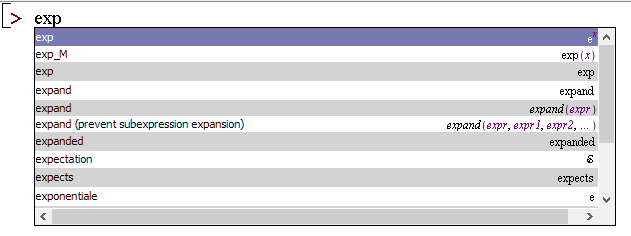
\includegraphics[width=\textwidth]{tutorials/figures/autocomplete.png}
\caption{Using autocomplete with ESC gives a menu of possible commands you are trying to use.}
\end{figure}
From here, you can select the \texttt{exp} command for the exponential function, or possibly the \texttt{expand} command, which we will look at later. If the command requires a parameter, it should already be highlighted so that you can type in its value. If a command has multiple parameters, you can hit the Tab key to highlight the next parameter.

\section{Multiple Commands at Once}

As you may have noticed, each time that we have used Maple input in this tutorial, there is a semicolon \texttt{;} at the end of the line. This used to be required in older versions of Maple, though it is no longer mandatory in modern versions.

\index{mathematical functions!exponential}
\index{mathematical functions!nth root@$n$\textsuperscript{th} root}

The reason why the semicolon continues to be important is because it tells Maple when one command ends and another begins. You can use this to run multiple commands within one Maple input:

\marginnote{Multiple commands can be run at the same time by placing a semicolon \texttt{;} in between them.}
\begin{maplegroup}
\begin{mapleinput}
\mapleinline{active}{1d}{surd(x,3); exp(x);
}{}
\end{mapleinput}
\mapleresult
\begin{maplelatex}
\mapleinline{inert}{2d}{surd(x,3)}{\[\displaystyle \sqrt[3]{x} \]}
\end{maplelatex}
\begin{maplelatex}
\mapleinline{inert}{2d}{exp(x)}{\[\displaystyle {\rm e}^{x} \]}
\end{maplelatex}
\end{maplegroup}
\marginnote{If you use a full colon \texttt{:} instead of a semicolon, then the output of that command is hidden from the screen when it is executed.}

\section{The \% Shortcut}\label{percentage}

\index{ditto operator}

Many of the exercises in the activities will involve executing multiple commands to obtain the answer. Often, this means running a command and then running a second command on the result of the first. Although copying and pasting the result from the first command takes less time than typing it out, it often causes many syntax problems.

Fortunately, Maple provides us with the \% shortcut, also called the ditto operator. Every time a command is run, its output is temporarily stored, much like a scientific calculator will remember what is currently on its screen. Using the \% symbol within another command will use the result of the first command automatically. 

The trouble with this shortcut comes from the fact that you can run Maple input anywhere on the page \textit{in any order}! In the example below, you will only get the correct output if you run the second line \textit{immediately} after running the first line.

\begin{maplegroup}
\begin{mapleinput}
\mapleinline{active}{1d}{x\symbol{94}2 + 5;
}{}
\end{mapleinput}
\mapleresult
\begin{maplelatex}
\mapleinline{inert}{2d}{x^2+5}{\[\displaystyle {x}^{2}+5\]}
\end{maplelatex}
\end{maplegroup}
\index{mathematical functions!square root}
\begin{maplegroup}
\begin{mapleinput}
\mapleinline{active}{1d}{sqrt(%);
}{}
\end{mapleinput}
\mapleresult
\begin{maplelatex}
\mapleinline{inert}{2d}{sqrt(x^2+5)}{\[\displaystyle \sqrt{{x}^{2}+5}\]}
\end{maplelatex}
\end{maplegroup}

To make better use of the \% shotcut, it is the best practice to combine the two consecutive commands on the same Maple input:

\marginnote{The \% shorcut in Maple works much like the \textit{ANS} button on many scientific calculators. The \% will only remember the output of whatever input was run most recently.}

\begin{maplegroup}
\begin{mapleinput}
\mapleinline{active}{1d}{x\symbol{94}2 - 4; sqrt(%);
}{}
\end{mapleinput}
\mapleresult
\begin{maplelatex}
\mapleinline{inert}{2d}{x^2-4}{\[\displaystyle {x}^{2}-4\]}
\end{maplelatex}
\begin{maplelatex}
\mapleinline{inert}{2d}{sqrt(x^2+5)}{\[\displaystyle \sqrt{{x}^{2}+5}\]}
\end{maplelatex}
\end{maplegroup}		
\chapter{Basic Operations}
\label{chp:basic_operations}

\section{Expressing a Result as a Decimal}

Maple tries to use exact, symbolic values whenever it can. If you need a decimal representation of a value or expression, you can use the \texttt{evalf()} command as seen below.

\index{evalf}
\index{mathematical functions!square root}
\index{Digits}
\index{Pi}

\begin{maplegroup}
\begin{mapleinput}
\mapleinline{active}{1d}{sqrt(2);
}{}
\end{mapleinput}
\mapleresult
\begin{maplelatex}
\mapleinline{inert}{2d}{sqrt(2)}{\[\displaystyle  \sqrt{2}\]}
\end{maplelatex}
\end{maplegroup}

\begin{maplegroup}
\begin{mapleinput}
\mapleinline{active}{1d}{evalf(sqrt(2));
}{}
\end{mapleinput}
\mapleresult
\begin{maplelatex}
\mapleinline{inert}{2d}{1.414213562}{\[\displaystyle  1.414213562\]}
\end{maplelatex}
\end{maplegroup}

\marginnote[-.8cm]{Maple will default to a decimal approximation anytime the input already uses decimals. For example, try \texttt{sqrt(2.0)} and see the result.}

It is often useful to give the exact value as well as the decimal approximation in one execution group, using the \% shortcut: 
\marginnote[.5cm]{Recall that using the \% symbol within another command will use the result of the first command automatically. } 

\begin{maplegroup}
\begin{mapleinput}
\mapleinline{active}{1d}{sqrt(2); evalf(%);
}{}
\end{mapleinput}
\mapleresult
\begin{maplelatex}
\mapleinline{inert}{2d}{sqrt(2)}{\[\displaystyle  \sqrt{2}\]}
\end{maplelatex}
\begin{maplelatex}
\mapleinline{inert}{2d}{1.414213562}{\[\displaystyle  1.414213562\]}
\end{maplelatex}
\end{maplegroup}

By default, Maple will express a decimal with $10$-digit accuracy. This default can be changed by assigning a new value to \texttt{Digits}, or you can specify the number of digits anytime you use the \texttt{evalf()} command.

\marginnote{The first letter of \texttt{Digits} must be capitalized and there must be a colon included before the equals sign.}

\begin{maplegroup}
\begin{mapleinput}
\mapleinline{active}{1d}{Digits := 15;
}{}
\end{mapleinput}
\mapleresult
\begin{maplelatex}
\mapleinline{inert}{2d}{Digits := 15}{\[\displaystyle {\it Digits}\, := \,15\]}
\end{maplelatex}
\end{maplegroup}

\marginnote{The assignment operator \texttt{:=} is explained in detail in Tutorial \ref{chp:assignment_operator} on page \pageref{chp:assignment_operator}.}

\begin{maplegroup}
\begin{mapleinput}
\mapleinline{active}{1d}{Pi;
}{}
\end{mapleinput}
\mapleresult
\begin{maplelatex}
\mapleinline{inert}{2d}{Pi}{\[\displaystyle \pi \]}
\end{maplelatex}
\end{maplegroup}

\begin{maplegroup}
\begin{mapleinput}
\mapleinline{active}{1d}{evalf(Pi);
}{}
\end{mapleinput}
\mapleresult
\begin{maplelatex}
\mapleinline{inert}{2d}{3.14159265358979}{\[\displaystyle  3.14159265358979\]}
\end{maplelatex}
\end{maplegroup}

\begin{maplegroup}
\begin{mapleinput}
\mapleinline{active}{1d}{evalf(Pi,50);
}{}
\end{mapleinput}
\mapleresult
\begin{maplelatex}
\mapleinline{inert}{2d}{3.1415926535897932384626433832795028841971693993751}{\[\displaystyle  3.1415926535897932384626433832795028841971693993751\]}
\end{maplelatex}
\end{maplegroup}

\section{Expanding Expressions}

You can ask Maple to expand any expression with the \texttt{expand()} command, including products of polynomials and rational functions. Maple will also expand various logarithmic and trigonometric expressions.

\index{expand}
\index{mathematical functions!cosine}
\index{mathematical functions!tangent}

\marginnote{The multiplication operation * (or a space in 2D Math mode) is not required between numerical coefficients and variable. However, multiplication between multiple variables is required.}
\begin{maplegroup}
\begin{mapleinput}
\mapleinline{active}{1d}{expand((2*x + 3*y)\symbol{94}6);
}{}
\end{mapleinput}
\mapleresult
\begin{maplelatex}
\mapleinline{inert}{2d}{64*x^6+576*x^5*y+2160*x^4*y^2+4320*x^3*y^3+4860*x^2*y^4+2916*x*y^5+729*y^6}{\[\displaystyle 64\,x^6+576\,x^5y+2160\,x^4y^2+4320\,x^3y^3+4860\,x^2y^4+2916\,xy^5+729\,y^6\]}
\end{maplelatex}
\end{maplegroup}

\begin{maplegroup}
\begin{mapleinput}
\mapleinline{active}{1d}{expand(cos(2*x));
}{}
\end{mapleinput}
\mapleresult
\begin{maplelatex}
\mapleinline{inert}{2d}{2*cos(x)^2-1}{\[\displaystyle 2\, \left( \cos \left( x \right)  \right) ^{2}-1\]}
\end{maplelatex}
\end{maplegroup}

\begin{maplegroup}
\begin{mapleinput}
\mapleinline{active}{1d}{expand(tan(a + b));
}{}
\end{mapleinput}
\mapleresult
\begin{maplelatex}
\mapleinline{inert}{2d}{(tan(a)+tan(b))/(1-tan(a)*tan(b))}{\[\displaystyle {\frac {\tan \left( a \right) +\tan \left( b \right) }{1-\tan \left( a \right) \tan \left( b \right) }}\]}
\end{maplelatex}
\end{maplegroup}


\section{Factoring Expressions}

Maple can also factor expressions with the \texttt{factor()} command. It will factor polynomials (including those with multiple variables) and will even factor more complicated expressions (like those involving trig functions as seen below).

\index{factor}
\index{mathematical functions!sine}

\begin{maplegroup}
\begin{mapleinput}
\mapleinline{active}{1d}{factor(x\symbol{94}2 - 1);
}{}
\end{mapleinput}
\mapleresult
\begin{maplelatex}
\mapleinline{inert}{2d}{(x-1)*(x+1)}{\[\displaystyle  \left( x-1 \right)  \left( x+1 \right) \]}
\end{maplelatex}
\end{maplegroup}

\marginnote[12pt]{In some cases, Maple may factor the expression and perform some additional basic simplification.}
\begin{maplegroup}
\begin{mapleinput}
\mapleinline{active}{1d}{factor((x\symbol{94}2 + 2*x - 15)/(x\symbol{94}2 + 7*x + 10));
}{}
\end{mapleinput}
\mapleresult
\begin{maplelatex}
\mapleinline{inert}{2d}{(x-1)/(x+1)}{\[\displaystyle  \frac{x-3}{x+2} \]}
\end{maplelatex}
\end{maplegroup}

\begin{maplegroup}
\begin{mapleinput}
\mapleinline{active}{1d}{factor(sin(x)\symbol{94}2 - 3*sin(x) + 2);
}{}
\end{mapleinput}
\mapleresult
\begin{maplelatex}
\mapleinline{inert}{2d}{(sin(x)-1)*(sin(x)-2)}{\[\displaystyle  \left( \sin \left( x \right) -1 \right)  \left( \sin \left( x \right) -2 \right) \]}
\end{maplelatex}
\end{maplegroup}

\marginnote{If Maple cannot factor the expression given, it will output the original expression.}

\begin{maplegroup}
\begin{mapleinput}
\mapleinline{active}{1d}{factor(x\symbol{94}2 + 1);
}{}
\end{mapleinput}
\mapleresult
\begin{maplelatex}
\mapleinline{inert}{2d}{x^2+1}{\[\displaystyle {x}^{2}+1\]}
\end{maplelatex}
\end{maplegroup}

Maple will factor expressions with multiple variables as well. Be sure to include multiplication (*) between variables.

\begin{maplegroup}
\begin{mapleinput}
\mapleinline{active}{1d}{factor(a\symbol{94}3 + 3*a\symbol{94}2*b + 3*a*b\symbol{94}2 + b\symbol{94}3);
}{}
\end{mapleinput}
\mapleresult
\begin{maplelatex}
\mapleinline{inert}{2d}{(a+b)^3}{\[\displaystyle (a+b)^3\]}
\end{maplelatex}
\end{maplegroup}

\section{Simplifying Expressions}

Likewise, you can also simplify any expression with \texttt{simplify()}. This includes basic simplifications such as collecting like terms as well as more complicated algebraic simplifications such as canceling and simplifying radicals, exponents, logarithms, trigonometric functions, etc.

\index{simplify}
\index{mathematical functions!sine}
\index{mathematical functions!cosine}
\index{mathematical functions!tangent}
\index{mathematical functions!logarithmic@natural logarithmic}

\begin{maplegroup}
\begin{mapleinput}
\mapleinline{active}{1d}{simplify(3*sin(x)\symbol{94}2 + 3*cos(x)\symbol{94}2);
}{}
\end{mapleinput}
\mapleresult
\begin{maplelatex}
\mapleinline{inert}{2d}{3}{\[\displaystyle 3\]}
\end{maplelatex}
\end{maplegroup}

\marginnote{The \texttt{simplify()} command can sometimes produce unexpected results. In some cases, the \texttt{factor} command may be more appropriate. In other cases, you may need to include some optional parameters in the command.}

\begin{maplegroup}
\begin{mapleinput}
\mapleinline{active}{1d}{simplify(4*(tan(x)\symbol{94}2 + 1));
}{}
\end{mapleinput}
\mapleresult
\begin{maplelatex}
\mapleinline{inert}{2d}{4/cos(x)^2}{\[\displaystyle 4\, \left( \cos \left( x \right)  \right) ^{-2}\]}
\end{maplelatex}
\end{maplegroup}

\begin{maplegroup}
\begin{mapleinput}
\mapleinline{active}{1d}{simplify(ln(3*x\symbol{94}3*y));
}{}
\end{mapleinput}
\mapleresult
\begin{maplelatex}
\mapleinline{inert}{2d}{ln(3)+ln(x^3*y)}{\[\displaystyle \ln  \left( 3 \right) +\ln  \left( {x}^{3}y \right) \]}
\end{maplelatex}
\end{maplegroup}

\marginnote{Sometimes additional parameters need to be supplied in order for Maple to simplify the expression as you intend. Here, we add the assumption that all variables are positive so that $\ln(x)$ and $\ln(y)$ are defined.}

\begin{maplegroup}
\begin{mapleinput}
\mapleinline{active}{1d}{simplify(ln(3*x\symbol{94}3*y), assume=positive);}{}
\end{mapleinput}
\mapleresult
\begin{maplelatex}
\mapleinline{inert}{2d}{ln(3)+3*ln(x)+ln(y)}{\[\displaystyle \ln  \left( 3 \right) +3\,\ln  \left( x \right) +\ln  \left( y \right) \]}
\end{maplelatex}
\end{maplegroup}
\chapter{Basics of Plotting}
\label{chp:plotting_functions}

\section{Plotting a Single Function}
\label{sec:plotting_a_single_function}

You can plot a function in Maple by using the \texttt{plot()} command. The only required parameter is the function you wish to plot. However, there are many additional parameters you can add to customise the way that the graph looks.

\marginnote{By default, Maple will plot trigonometric functions with an $x$-axis from $-2\pi$ to $2\pi$.}

\begin{maplegroup}
\begin{mapleinput}
\mapleinline{active}{1d}{plot(sin(cos(x)));
}{}
\index{plot}
\end{mapleinput}
\mapleresult
\mapleplot{tutorials/figures/Plotting_Functionsplot2d1a-eps-converted-to.pdf}
\end{maplegroup}

It is often useful to specify the interval for the $x$-axis. Choose left and right endpoint for the $x$-axis that are appropriate for your graph.\index{plot!axes intervals}

\marginnote{If you are plotting a function of $t$, then make sure to specify the interval as \texttt{t=a..b}.}

\begin{maplegroup}
\begin{mapleinput}
\mapleinline{active}{1d}{plot(sin(cos(x)), x=-10..10);
}{}
\end{mapleinput}
\mapleresult
\mapleplot{tutorials/figures/Plotting_Functionsplot2d1b-eps-converted-to.pdf}
\end{maplegroup}

\marginnote[1cm]{The order of the parameters in the \texttt{plot()} command is important. The interval for the $x$-axis must be listed before the interval for the $y$-axis.}
You can also specify the interval for the $y$-axis for your graph.\index{plot!axes intervals}

\begin{maplegroup}
\begin{mapleinput}
\mapleinline{active}{1d}{plot(sin(cos(x)), x=-10..10, y=-5..5);\index{plot!axes intervals}
}{}
\end{mapleinput}
\mapleresult
\mapleplot{tutorials/figures/Plotting_Functionsplot2d1c-eps-converted-to.pdf}
\end{maplegroup}

\section{Common Plot Options}
\label{sec:common_plot_options}

Table \ref{tbl:plot_options} lists the most frequently used optional parameters.

\begin{table}
\label{tbl:plot_options}
\centering
\begin{tabular}{lp{2.5in}}
\hline
Parameter & Description\\
\hline
\texttt{x=a..b}						& Plot over the interval $x\in[a,b]$.
    \index{plot!axes intervals}
    \\
\texttt{y=c..d}						& Plot over the interval $y\in[c,d]$.
    \index{plot!axes intervals}
    \\
\texttt{colour=}\textit{cname}		& Specify the colour of the graph.
    \index{plot!colours}
    \\
\texttt{discont=true}				& Show discontinuities in a function.
    \index{plot!axes intervals}
    \index{plot!discontinuities}
    \\
\texttt{linestyle=}\textit{lstyle}	& Specify the style of the line (\texttt{solid}, \texttt{dash}, \texttt{dot}, etc.).
    \index{plot!line style}
    \\
\texttt{gridlines=true}				& Include gridlines.
    \index{plot!gridlines}
    \\
\texttt{numpoints=}\textit{n}		& Set the minimum number of points plotted for a smoother graph (Default $200$).
    \index{plot!plot resolution}
    \\
\texttt{grid=[$m$,$n$]}				& Set the number of initial points used to plot a graph (Default $26 \times 26$).
    \index{plot!plot resolution}
    \\
\texttt{scaling=constrained}		& Force axes to use the same scale (so a circle should appear perfectly round).
    \index{plot!scaling}
    \\
\hline
\end{tabular}
\caption{A list of common optional parameters for the \texttt{plot()} command.}
\end{table}
\marginnote[-6cm]{A list of plot colours can be found by typing \texttt{?colours} on a new Maple input.}
\marginnote[-4cm]{Plotting commands often generate more than the minimum number of points. Setting \texttt{numpoints = 30000} may help if a graph does not appear smooth. Using too large of a value may cause Maple to become unresponsive (see Tutorial \ref{chp:implicit_functions}).}

The \texttt{discont=true} parameter may need to be included to properly display the discontinuities in certain functions when you plot them.

\begin{marginfigure}[-.1cm]
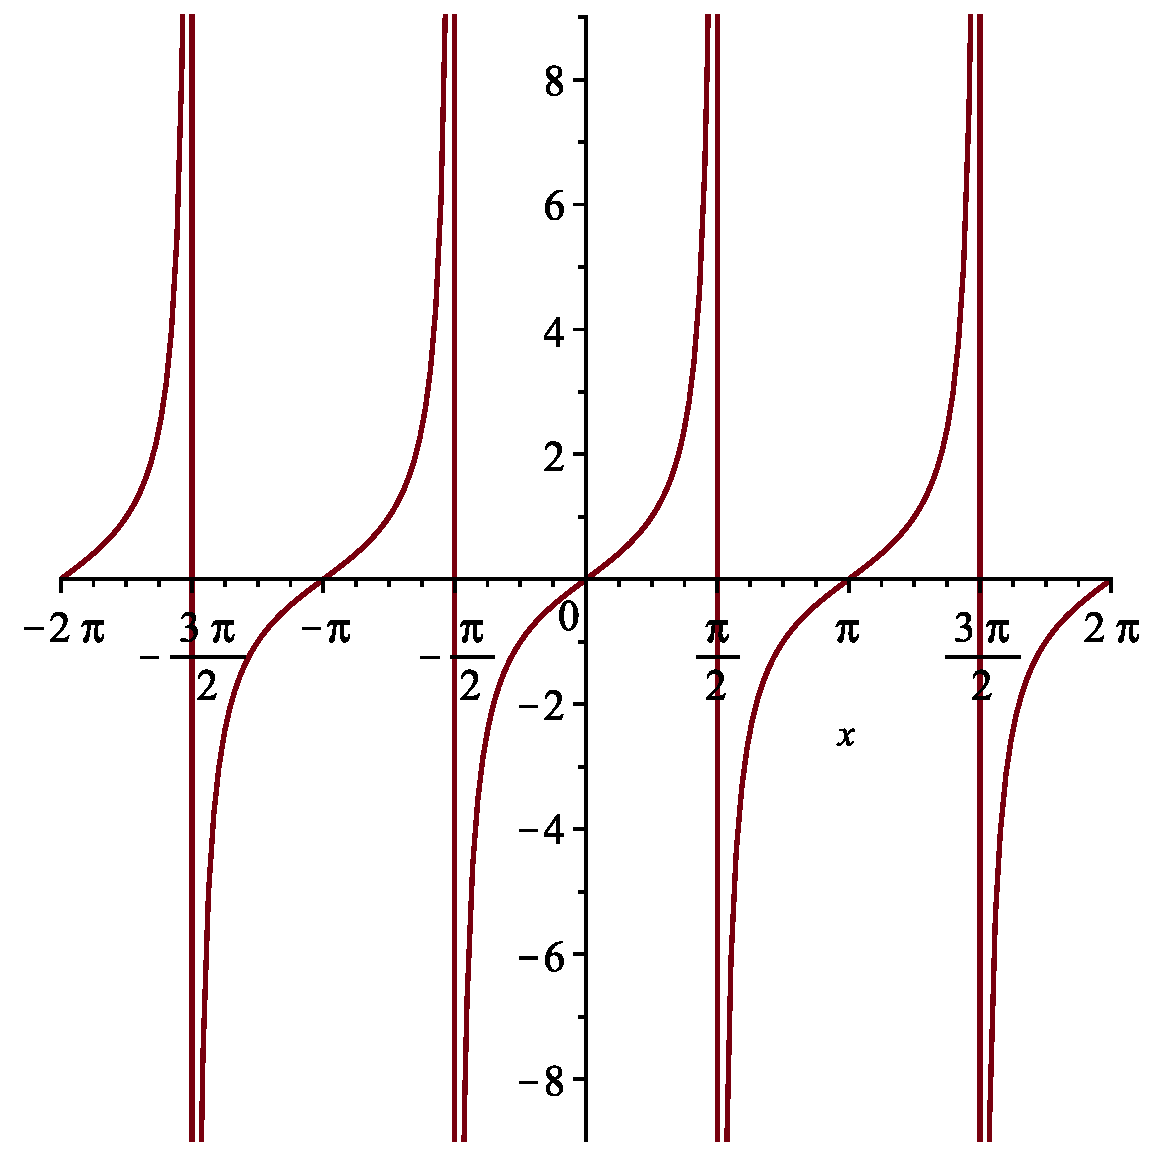
\includegraphics[width=5cm]{tutorials/figures/Plotting_Functionsplot2d2b-eps-converted-to.pdf}
\caption{Some versions of Maple may not correctly display the discontinuities in the graph of $\tan(x)$, as shown here. In this case, you need to include the \texttt{discont=true} parameter. Notice that the \texttt{linestyle=dashed} option was also excluded here.}
\end{marginfigure}

\begin{maplegroup}
\begin{mapleinput}
\mapleinline{active}{1d}{plot(tan(x), x=-2*Pi..2*Pi, y=-10..10, linestyle=dash, discont=true);
}{}
\end{mapleinput}
\mapleresult
\mapleplot{tutorials/figures/Plotting_Functionsplot2d3-eps-converted-to.pdf}
\end{maplegroup}
\begin{marginfigure}[-.8cm]
An example of a function that cannot be properly displayed without the \texttt{discont=true} parameter can be found on page \pageref{sec:limits_and_piecewise_functions}.
\end{marginfigure}
In some modern versions of Maple, the graph of $\tan(x)$ above can be obtained even without including the \texttt{discont=true} option in the \texttt{plot( )} command.

\section{Plotting Multiple Functions}
\label{sec:plotting_multiple_functions}

You can also plot multiple expressions and functions on the same graph using the \texttt{plot()} command. Instead of specifying a single function as your first parameter, create a list of functions using square brackets.

Similarly, instead of specifying a single colour, specify a list of colours using square brackets. The order of the functions matches the order of the colours.

\marginnote{If a list of colours is not specified when plotting multiple functions on the same graph, it may be difficult to match each curve to its corresponding function. The first three colours in Maple's default palette are dull shades of red, blue, and green.}
\begin{maplegroup}
\begin{mapleinput}
\mapleinline{active}{1d}{plot([exp(x), sin(x) + cos(x)], x=-10..10, y=-5..5, colour=[black, blue]);
}{}
\label{Plot!Plot multiple functions}
\end{mapleinput}
\mapleresult
\mapleplot{tutorials/figures/Plotting_Functionsplot2d2a-eps-converted-to.pdf}
\end{maplegroup}

If you need several complicated graphs to display at once, you may wish to explore the potential of the \texttt{display()} command, found in section \ref{sec:display_command} on page \pageref{sec:display_command}.
\chapter{The Assignment Operator and Defining Functions}
\label{chp:assignment_operator}

\section{Assigning Expressions}
\label{sec:assigning_expressions}

Having to retype the same expression multiple times is tedious, but using copy and paste in Maple can sometimes produce unwanted effects. A better way to reuse an expression multiple times is to assign a name to it. You can assign any expression to a name of your choice (with some exceptions that Maple has protected) by using the \text{:=} operator.
\index{assignment operator}
\index{mathematical functions!exponential}
\index{mathematical functions!square root}
\marginnote{Protected names include common functions such as \texttt{exp}. For example, \begin{center}\texttt{> exp := 2*x;}\end{center} would cause an error.}

\begin{maplegroup}
\begin{mapleinput}
\mapleinline{active}{1d}{poly := 3*x\symbol{94}4 - 2*x + 1;
}{}
\end{mapleinput}
\mapleresult
\begin{maplelatex}
\mapleinline{inert}{2d}{poly := 3*x^4-2*x+1}{\[\displaystyle {\it poly}\, := \,3\,{x}^{4}-2\,x+1\]}
\end{maplelatex}
\end{maplegroup}

\begin{maplegroup}
\begin{mapleinput}
\mapleinline{active}{1d}{poly;
}{}
\end{mapleinput}
\mapleresult
\begin{maplelatex}
\mapleinline{inert}{2d}{3*x^4-2*x+1}{\[\displaystyle 3\,{x}^{4}-2\,x+1\]}
\end{maplelatex}
\end{maplegroup}

\marginnote[0.5cm]{Never assign anything to single-letter names such as $x$ or $y$. It is best to keep single letters as arbitrary variables.}
\begin{maplegroup}
\begin{mapleinput}
\mapleinline{active}{1d}{poly\symbol{94}2;
}{}
\end{mapleinput}
\mapleresult
\begin{maplelatex}
\mapleinline{inert}{2d}{(3*x^4-2*x+1)^2}{\[\displaystyle  \left( 3\,{x}^{4}-2\,x+1 \right) ^{2}\]}
\end{maplelatex}
\end{maplegroup}

\begin{maplegroup}
\begin{mapleinput}
\mapleinline{active}{1d}{expr := (4\symbol{94}x - x\symbol{94}4) / exp(x + 1);
}{}
\end{mapleinput}
\mapleresult
\begin{maplelatex}
\mapleinline{inert}{2d}{expr:=(4^x-x^4)/exp(x+1)}{\[\displaystyle {\it expr}\, := \,{\frac {{4}^{x}-{x}^{4}}{{{\rm e}^{x+1}}}}\]}
\end{maplelatex}
\end{maplegroup}

\marginnote{It is important to assign expressions to names that make sense to you and are easy to remember. It is also recommended not to reuse a name in the same document. If you assign a new expression to an old name, the new expression will overwrite what was previously assigned.}
\begin{maplegroup}
\begin{mapleinput}
\mapleinline{active}{1d}{expr;
}{}
\end{mapleinput}
\mapleresult
\begin{maplelatex}
\mapleinline{inert}{2d}{(4^x-x^4)/exp(x+1)}{\[\displaystyle {\frac {{4}^{x}-{x}^{4}}{{{\rm e}^{x+1}}}}\]}
\end{maplelatex}
\end{maplegroup}

\begin{maplegroup}
\begin{mapleinput}
\mapleinline{active}{1d}{sqrt(expr);
}{}
\end{mapleinput}
\mapleresult
\begin{maplelatex}
\mapleinline{inert}{2d}{sqrt((4^x-x^4)/exp(x+1))}{\[\displaystyle  \sqrt{{\frac {{4}^{x}-{x}^{4}}{{{\rm e}^{x+1}}}}}\]}
\end{maplelatex}
\end{maplegroup}

\section{Making a Substitution into an Expression}
\label{sec:making_substitutions}

Let's suppose you have assigned an expression a name, and wish to replace one of its variables with a value or expression. As an example, we will assign an expression a name of \texttt{expr} and then substitute the numerical value for $\pi$, which is denoted as \texttt{Pi} in Maple, into \texttt{expr}. The command used to substitute a value into an expression is \texttt{subs()}.

\begin{maplegroup}
\begin{mapleinput}
\mapleinline{active}{1d}{expr := sin(x) - 1;
}{}
\end{mapleinput}
\mapleresult
\begin{maplelatex}
\mapleinline{inert}{2d}{expr := sin(x)-1}{\[\displaystyle {\it expr}\, := \,\sin \left( x \right) -1\]}
\end{maplelatex}
\end{maplegroup}
\marginnote[-.2cm]{Always be sure to use a capital P in \texttt{Pi} for the mathematical constant. You can also find $\pi$ in the palettes toolbar.}
\index{Pi}
\index{mathematical functions!sine}
\index{mathematical functions!exponential}
\index{ditto operator}
\index{mathematical functions!tangent}


\begin{maplegroup}
\begin{mapleinput}
\mapleinline{active}{1d}{subs(x = Pi, expr);
}{}
\end{mapleinput}
\mapleresult
\begin{maplelatex}
\mapleinline{inert}{2d}{sin(Pi)-1}{\[\displaystyle \sin \left( \pi  \right) -1\]}
\end{maplelatex}
\end{maplegroup}
\marginnote[0.1cm]{The order of the parameters in the \texttt{subs()} command is important. For example, \begin{center}\texttt{> subs(expr,x = Pi);}\end{center} would cause an error.}
You can make use of the \% shortcut if you wish, but recall that it is best used on the same Maple input:

\begin{maplegroup}
\begin{mapleinput}
\mapleinline{active}{1d}{x\symbol{94}2 + 3*x - 4; subs(x = 2, %);
}{}
\end{mapleinput}
\mapleresult\begin{maplelatex}
\mapleinline{inert}{2d}{x^2+3*x-4}{\[\displaystyle {x}^{2}+3\,x-4\]}
\end{maplelatex}
\begin{maplelatex}
\mapleinline{inert}{2d}{6}{\[\displaystyle 6\]}
\end{maplelatex}
\end{maplegroup}



You can also substitute one expression into another:
\marginnote{Note that using the \texttt{subs()} command does not permanently assign the substitution.}
\begin{maplegroup}
\begin{mapleinput}
\mapleinline{active}{1d}{expr2 := tan(2*x) + 1;
}{}
\end{mapleinput}
\mapleresult
\begin{maplelatex}
\mapleinline{inert}{2d}{expr2 := tan(2*x)+1}{\[\displaystyle {\it expr2}\, := \,\tan \left( 2\,x \right) +1\]}
\end{maplelatex}
\end{maplegroup}

\begin{maplegroup}
\begin{mapleinput}
\mapleinline{active}{1d}{subs(x = a+h, expr2);
}{}
\end{mapleinput}
\mapleresult
\begin{maplelatex}
\mapleinline{inert}{2d}{tan(2*a+2*h)+1}{\[\displaystyle \tan \left( 2\,a+2\,h \right) +1\]}
\end{maplelatex}
\end{maplegroup}
\begin{maplegroup}
\begin{mapleinput}
\mapleinline{active}{1d}{}{}
\end{mapleinput}
\end{maplegroup}

\section{Defining a Function}
\label{sec:define_function}

Instead of defining an expression, it is sometimes more useful to define a function. A function specifies the variables that are included in the expression. This allows us to substitute values into our functions easily using function notation, such as $f(5)$.

\marginnote[-0.5cm]{If you have properly defined a function, you should see an arrow ($\rightarrow$) in your output. If you do not see an arrow within the output, then you have not defined the function properly.}

\begin{maplegroup}
\begin{mapleinput}
\mapleinline{active}{1d}{f(x) := sin(x) - exp(x);
}{}
\end{mapleinput}
\mapleresult
\begin{maplelatex}
\mapleinline{inert}{2d}{f := proc (x) options operator, arrow; sin(x)-exp(x) end proc}{\[\displaystyle f\, := \,x\mapsto \sin \left( x \right) -{{\rm e}^{x}}\]}
\end{maplelatex}
\end{maplegroup}

\marginnote[0.5cm]{Make sure that the variable in the function name matches the variable in the function.}

\begin{maplegroup}
\begin{mapleinput}
\mapleinline{active}{1d}{g(t) := -4.9*t\symbol{94}2 + 5*t + 20;
}{}
\end{mapleinput}
\mapleresult
\begin{maplelatex}
\mapleinline{inert}{2d}{g := proc (t) options operator, arrow; (-1)*4.9*t^2+5*t+20 end proc}{\[\displaystyle g\, := \,t\mapsto - 4.9\,{t}^{2}+5\,t+20\]}
\end{maplelatex}
\end{maplegroup}

A function's name does not have to be a single letter. In fact, it is often a good idea to have a function's name correspond to what the function represents.

\begin{maplegroup}
\begin{mapleinput}
\mapleinline{active}{1d}{area(r) := Pi*r\symbol{94}2;
}{}
\end{mapleinput}
\mapleresult
\begin{maplelatex}
\mapleinline{inert}{2d}{area := proc (r) options operator, arrow; Pi*r^2 end proc}{\[\displaystyle {\it area}\, := \,r\mapsto \pi\,{r}^{2}\]}
\end{maplelatex}
\end{maplegroup}

\begin{marginfigure}
\centering
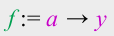
\includegraphics[scale=0.8]{tutorials/figures/palettefunc.png}
\caption{You can find a shortcut for defining functions in the palettes toolbar under Expression. This button makes use of the arrow notation.}
\end{marginfigure}

\section{Using Function Notation}
\label{sec:function_notation}

Once we have defined a function, we can use function notation much like we would in class. For example, instead of defining an expression involving $x$ to a name such as \texttt{expr} and then using the \texttt{subs()} command to substitute $x=0$ into \texttt{expr}, we can now use the function $f(x)$ as assigned in Section \ref{sec:define_function} and type $f(0)$.

\begin{maplegroup}
\begin{mapleinput}
\mapleinline{active}{1d}{f(0);
}{}
\end{mapleinput}
\mapleresult
\begin{maplelatex}
\mapleinline{inert}{2d}{-1}{\[\displaystyle -1\]}
\end{maplelatex}
\end{maplegroup}

It is easy to substitute an expression into a function using function notation.

\begin{maplegroup}
\begin{mapleinput}
\mapleinline{active}{1d}{g(x) := 2*x\symbol{94}2 - 3*x;
}{}
\end{mapleinput}
\mapleresult
\begin{maplelatex}
\mapleinline{inert}{2d}{g := proc (x) options operator, arrow; 2*x^2-3*x end proc}{\[\displaystyle g\, := \,x\mapsto 2\,{x}^{2}-3\,x\]}
\end{maplelatex}
\end{maplegroup}

\begin{maplegroup}
\begin{mapleinput}
\mapleinline{active}{1d}{g(x+1);
}{}
\end{mapleinput}
\mapleresult
\begin{maplelatex}
\mapleinline{inert}{2d}{2*(x+1)^2-3*x-3}{\[\displaystyle 2\, \left( x+1 \right) ^{2}-3\,x-3\]}
\end{maplelatex}
\end{maplegroup}

\section{Operations on Functions}
\label{sec:operations_on_functions}

Once one or more functions are assigned, we can make expressions using function notation, or perform other operations on those functions.

\begin{maplegroup}
\begin{mapleinput}
\mapleinline{active}{1d}{f(x) := 2*x\symbol{94}3;
}{}
\end{mapleinput}
\mapleresult
\begin{maplelatex}
\mapleinline{inert}{2d}{f := proc (x) options operator, arrow; 2*x^3 end proc}{\[\displaystyle f\, := \,x\mapsto 2\,{x}^{3}\]}
\end{maplelatex}
\end{maplegroup}
\begin{maplegroup}
\begin{mapleinput}
\mapleinline{active}{1d}{g(t) := t+1;
}{}
\end{mapleinput}
\mapleresult
\begin{maplelatex}
\mapleinline{inert}{2d}{g := proc (t) options operator, arrow; t+1 end proc}{\[\displaystyle g\, := \,t\mapsto t+1\]}
\end{maplelatex}
\end{maplegroup}
\begin{maplegroup}
\begin{mapleinput}
\mapleinline{active}{1d}{f(g(t)); expand(%);
}{}
\end{mapleinput}
\mapleresult
\begin{maplelatex}
\mapleinline{inert}{2d}{2*(t+1)^3}{\[\displaystyle 2\, \left( t+1 \right) ^{3}\]}
\end{maplelatex}
\mapleresult
\begin{maplelatex}
\mapleinline{inert}{2d}{2*t^3+6*t^2+6*t+2}{\[\displaystyle 2\,{t}^{3}+6\,{t}^{2}+6\,t+2\]}
\end{maplelatex}
\end{maplegroup}
\begin{maplegroup}
\begin{mapleinput}
\mapleinline{active}{1d}{plot(f(x), x=-5..5);
}{}
\end{mapleinput}
\mapleresult
\mapleplot{tutorials/figures/funtionnotationplot2d1-eps-converted-to.pdf}
\end{maplegroup}

\index{expand}
\index{plot}
\index{plot!axes intervals}

\subsection{Average Rate of Change of a Function over an Interval}

In this example, we will find the average rate of change of the function $f(x) = -2x^3 + 25x^2 + 15$ over the interval $[2,7]$. We begin by defining the function:

\begin{maplegroup}
\begin{mapleinput}
\mapleinline{active}{1d}{f(x) := -2*x\symbol{94}3 + 25*x\symbol{94}2 + 15;
}{}
\end{mapleinput}
\mapleresult
\begin{maplelatex}
\mapleinline{inert}{2d}{f := proc (x) options operator, arrow; -2*x^3+25*x^2+15 end proc}{\[\displaystyle f\, := \,x\mapsto -2\,{x}^{3}+25\,{x}^{2}+15\]}
\end{maplelatex}
\end{maplegroup}

Once the function is defined, we can calculate the average rate of change over an interval $[a,b]$ by using the formula \[ \frac{f(b)-f(a)}{b-a}. \] 
In this case, we let $a=2$ and $b=7$:

\marginnote{This fraction will look much nicer on your screen if you use 2D Math font.}
\begin{maplegroup}
\begin{mapleinput}
\mapleinline{active}{1d}{(f(7) - f(2))/(7 - 2);
}{}
\end{mapleinput}
\mapleresult
\begin{maplelatex}
\mapleinline{inert}{2d}{91}{\[\displaystyle 91\]}
\end{maplelatex}
\end{maplegroup}
\begin{maplegroup}
\begin{mapleinput}
\mapleinline{active}{1d}{}{}
\end{mapleinput}
\end{maplegroup}

\noindent
The average rate of change over the interval $[2,7]$ is $91$. The units of this rate would be given in (units of $y$)/(units of $x$).

\subsection{Plotting Transformations of Functions}
\label{subsec:plotting_transformations}

Suppose that we start with a sinusoidal function $g(x)$ with amplitude $2$ and period $2$.

\begin{maplegroup}
\begin{mapleinput}
\mapleinline{active}{1d}{g(x) := 2*sin(Pi*x);
}{}
\end{mapleinput}
\end{maplegroup}

\begin{maplegroup}
\begin{mapleinput}
\mapleinline{active}{1d}{plot(g(x), x=0..4, y=-4..4);
}{}
\end{mapleinput}
\mapleresult
\mapleplot{tutorials/figures/transformationsplot2d1-eps-converted-to.pdf}
\end{maplegroup}

\index{plot}
\index{Pi}
\index{plot!axes intervals}
\index{plot!multiple functions}

We can then plot the original function $g(x)$ and and the transformation $\frac{1}{2}g(x)$ on the same axes to see that the amplitude has been halved.

\begin{maplegroup}
\begin{mapleinput}
\mapleinline{active}{1d}{plot([g(x), 0.5*g(x)], x=0..4, y=-4..4);
}{}
\end{mapleinput}
\mapleresult
\mapleplot{tutorials/figures/transformationsplot2d2-eps-converted-to.pdf}
\end{maplegroup}

We can also see how an absolute value transformation of $g(x)$ compares to the original function. The result here is known as a fully rectified sine wave.

\begin{maplegroup}
\begin{mapleinput}
\mapleinline{active}{1d}{plot([ g(x), abs(g(x)) ], x=0..4, y=-4..4);
}{}
\end{mapleinput}
\mapleresult
\mapleplot{tutorials/figures/transformationsplot2d3-eps-converted-to.pdf}
\end{maplegroup}

\index{mathematical functions!absolute value}
\index{plot!axes intervals}
\index{plot!multiple functions}

\section{Assigning Piecewise Functions}
\label{sec:piecewise}

A piecewise-defined function is a function defined by multiple sub-functions. Each sub-function applies to a certain interval of the domain, called a sub-domain. We can define piecewise functions in Maple by using the \texttt{piecewise()} command. The sub-domain of each sub-function is specified before its expression.

\index{mathematical functions!piecewise}

\begin{maplegroup}
\begin{mapleinput}
\mapleinline{active}{1d}{P(x) := piecewise(x<=-1, x\symbol{94}2, -1<x<=1, -x, 1<x, x-4);
}{}
\index{mathematical functions!piecewise}
\end{mapleinput}
\mapleresult
\begin{maplelatex}
\mapleinline{inert}{2d}{P := proc (x) options operator, arrow; piecewise(x <= -1, x^2, -1 < x <= 1, -x, 1 < x, x-4) end proc}{\[\displaystyle P\, := \,x\mapsto \begin{cases}{x}^{2}&x\leq -1 \\ -x&-1< x\leq 1 \\ x-4&1<x\end{cases}\]}
\end{maplelatex}
\end{maplegroup}

\begin{maplegroup}
\begin{mapleinput}
\mapleinline{active}{1d}{P(x);
}{}
\end{mapleinput}
\mapleresult
\begin{maplelatex}
\mapleinline{inert}{2d}{piecewise(x <= -1, x^2, -1 < x <= 1, -x, 1 < x, x-4)}{\[\displaystyle \begin{cases}{x}^{2}& x\leq -1 \\ -x& -1 < x\leq 1 \\ x-4&1<x\end{cases}\]}
\end{maplelatex}
\end{maplegroup}

\section{Functions of More than One Variable}
\label{sec:functions_multiple_variables}

We can also define functions of multiple variables and use the notation the same way as one variable functions.

\index{mathematical functions!sine}
\index{mathematical functions!cosine}
\index{mathematical functions!multivariable functions}

\begin{maplegroup}
\begin{mapleinput}
\mapleinline{active}{1d}{g(x,y) := sin(x) - cos(y);
}{}
\end{mapleinput}
\mapleresult
\begin{maplelatex}
\mapleinline{inert}{2d}{g := proc (x, y) options operator, arrow; sin(x)-cos(y) end proc}{\[\displaystyle g\, := \,( {x,y} )\mapsto \sin \left( x \right) -\cos \left( y \right) \]}
\end{maplelatex}
\end{maplegroup}

\noindent
Evaluating at a point:

\begin{maplegroup}
\begin{mapleinput}
\mapleinline{active}{1d}{g(0, Pi);
}{}
\end{mapleinput}
\mapleresult
\begin{maplelatex}
\mapleinline{inert}{2d}{1}{\[\displaystyle 1\]}
\end{maplelatex}
\end{maplegroup}

\index{Pi}

An example of a function of more than one variable is the volume of a circular cylinder.

\begin{maplegroup}
\begin{mapleinput}
\mapleinline{active}{1d}{cylindervol(r,h) := Pi*r\symbol{94}2*h;
}{}
\end{mapleinput}
\mapleresult
\begin{maplelatex}
\mapleinline{inert}{2d}{cylindervol := proc (r, h) options operator, arrow; Pi*r^2*h end proc}{\[\displaystyle {\it cylindervol}\, := \,( {r,h} )\mapsto \pi\,{r}^{2}h\]}
\end{maplelatex}
\end{maplegroup}

\begin{maplegroup}
\begin{mapleinput}
\mapleinline{active}{1d}{cylindervol(3,5);
}{}
\end{mapleinput}
\mapleresult
\begin{maplelatex}
\mapleinline{inert}{2d}{45*Pi}{\[\displaystyle 45\,\pi\]}
\end{maplelatex}
\end{maplegroup}

\section{Assigning Plots and the \texttt{display()} Command}
\label{sec:display_command}

You can use the assignment operator to assign just about any type of output to a variable name, including plots. This can be useful when different types of plots need to be displayed on the same graph. You can assign the output of several \texttt{plot()} commands to variables and then 'display' them all on the same set of axes. 

To make use of the \texttt{display()} command, you need to include the \texttt{plots} package. Packages are loaded using the \texttt{with()} command, where the name of the package appears within the parentheses. The command
\index{packages!plots}
\index{packages!with}
\begin{maplegroup}
\begin{mapleinput}
\mapleinline{active}{1d}{with(plots);
}{}
\end{mapleinput}
\mapleresult
\begin{maplelatex}
\mapleinline{inert}{2d}{[plots:-animate, plots:-animate3d, plots:-animatecurve, plots:-arrow, plots:-changecoords, plots:-complexplot, plots:-complexplot3d, plots:-conformal, plots:-conformal3d, plots:-contourplot, plots:-contourplot3d, plots:-coordplot, plots:-coordplot3d, plots:-densityplot, plots:-display, plots:-dualaxisplot, plots:-fieldplot, plots:-fieldplot3d, plots:-gradplot, plots:-gradplot3d, plots:-implicitplot, plots:-implicitplot3d, plots:-inequal, plots:-interactive, plots:-interactiveparams, plots:-intersectplot, plots:-listcontplot, plots:-listcontplot3d, plots:-listdensityplot, plots:-listplot, plots:-listplot3d, plots:-loglogplot, plots:-logplot, plots:-matrixplot, plots:-multiple, plots:-odeplot, plots:-pareto, plots:-plotcompare, plots:-pointplot, plots:-pointplot3d, plots:-polarplot, plots:-polygonplot, plots:-polygonplot3d, plots:-polyhedra_supported, plots:-polyhedraplot, plots:-rootlocus, plots:-semilogplot, plots:-setcolors, plots:-setoptions, plots:-setoptions3d, plots:-shadebetween, plots:-spacecurve, plots:-sparsematrixplot, plots:-surfdata, plots:-textplot, plots:-textplot3d, plots:-tubeplot]}{\[\displaystyle [{\it animate},{\it animate3d},{\it animatecurve}
\hdots
\mbox{}]\]}
\end{maplelatex}
\end{maplegroup}
\noindent
will display all of the commands that are included in the package. If a full colon is added, then the package is loaded but the output is hidden.

\begin{maplegroup}
\begin{mapleinput}
\mapleinline{active}{1d}{with(plots):
}{}
\end{mapleinput}
\end{maplegroup}

With the \texttt{plots} package loaded, plotting options can be defined for each plot individually and assigned to a name. Multiple plots can then be displayed together.

\marginnote{A package does not need to be loaded more than once in your document. However, you will need to reload the package if you have previously closed the document.}
\begin{maplegroup}
\begin{mapleinput}
\mapleinline{active}{1d}{p1(x) := (x+2)\symbol{94}2 + 2*(x+2) - 5;
p2(x) := 3*(x-4)\symbol{94}3 - 2*(x-4)\symbol{94}2 - (x-4) + 1;
p3(x) := x - 3;
}{}
\end{mapleinput}
\mapleresult
\begin{maplelatex}
\mapleinline{inert}{2d}{p1 := proc (x) options operator, arrow; (x+2)^2+2*x-1 end proc}{\[\displaystyle {\it p1}\, := \,x\mapsto  \left( x+2 \right) ^{2}+2\,x-1\]}
\end{maplelatex}
\mapleresult
\begin{maplelatex}
\mapleinline{inert}{2d}{p2 := proc (x) options operator, arrow; 3*(x-4)^3-2*(x-4)^2-x+5 end proc}{\[\displaystyle {\it p2}\, := \,x\mapsto 3\, \left( x-4 \right) ^{3}-2\, \left( x-4 \right) ^{2}-x+5\]}
\end{maplelatex}
\mapleresult
\begin{maplelatex}
\mapleinline{inert}{2d}{p3 := proc (x) options operator, arrow; x-3 end proc}{\[\displaystyle {\it p3}\, := \,x\mapsto x-3\]}
\end{maplelatex}
\end{maplegroup}

\index{plot}
\index{plot!axes intervals}
\index{plot!line style}
\index{display}

\marginnote[0.5cm]{Full colons are used at the end of each line here to hide the output of the individual plot.}
\begin{maplegroup}
\begin{mapleinput}
\mapleinline{active}{1d}{A := plot(p1(x), x=-6..0, y=-6..3, linestyle=dot):
}{}
\end{mapleinput}
\end{maplegroup}
\begin{maplegroup}
\begin{mapleinput}
\mapleinline{active}{1d}{B := plot(p2(x), x=-0..10, y=-10..10, style=point):
}{}
\end{mapleinput}
\end{maplegroup}
\begin{maplegroup}
\begin{mapleinput}
\mapleinline{active}{1d}{C := plot(p3(x), x=-10..10, y=-10..10):
}{}
\end{mapleinput}
\end{maplegroup}
\begin{maplegroup}
\begin{mapleinput}
\mapleinline{active}{1d}{display([A,B,C]);
}{}
\end{mapleinput}
\mapleresult
\mapleplot{tutorials/figures/Plotting_Functionsplot2d4-eps-converted-to.pdf}
\end{maplegroup}
\begin{maplegroup}
\begin{mapleinput}
\mapleinline{active}{1d}{}{}
\end{mapleinput}
\end{maplegroup}
\begin{Maple Normal}{
\begin{Maple Normal}{
\mapleinline{inert}{2d}{}{\[\displaystyle \]}
}\end{Maple Normal}
}\end{Maple Normal}
\begin{Maple Normal}{
\begin{Maple Normal}{
\mapleinline{inert}{2d}{}{\[\displaystyle \]}
}\end{Maple Normal}
}\end{Maple Normal}
\chapter{Equation Solvers}
\label{chp:equation_solvers}		

\section{Assigning Equations}

The assignment operator \text{:=} can be used to assign a name to nearly any type of output. Often, it is useful to assign an equation (involving a regular $=$ sign) a name. Some of the operations that we discussed in Tutorial \ref{chp:basic_operations} (such as simplifying, expanding, substituting, etc.) can then be applied to that equation.

\index{subs}
\index{factor}
\index{solving equations!solve}
\index{solving equations!fsolve}

\begin{maplegroup}
\begin{mapleinput}
\mapleinline{active}{1d}{circle := x\symbol{94}2 + y\symbol{94}2 = 25;
}{}
\end{mapleinput}
\mapleresult
\begin{maplelatex}
\mapleinline{inert}{2d}{circle:=x^2+y^2 = 25}{\[\displaystyle {\it circle}\, := \,{x}^{2}+{y}^{2}=25\]}
\end{maplelatex}
\end{maplegroup}

\marginnote[-.5cm]{Recall that $x^2+y^2=25$ represents a circle of radius 5 centred at the origin. The point $(3,4)$ lies on this circle because $x=3$ and $y=4$ satisfy the equation.}

\begin{maplegroup}
\begin{mapleinput}
\mapleinline{active}{1d}{subs(x = 3, y = 4, circle);
}{}
\end{mapleinput}
\mapleresult
\begin{maplelatex}
\mapleinline{inert}{2d}{25 = 25}{\[\displaystyle 25=25\]}
\end{maplelatex}
\end{maplegroup}

\begin{maplegroup}
\begin{mapleinput}
\mapleinline{active}{1d}{eqn := x\symbol{94}4 + 1 = 2*x\symbol{94}2;
}{}
\end{mapleinput}
\mapleresult
\begin{maplelatex}
\mapleinline{inert}{2d}{eqn := x^4+1 = 2*x^2}{\[\displaystyle {\it eqn}\, := \,{x}^{4}+1=2\,{x}^{2}\]}
\end{maplelatex}
\end{maplegroup}

\marginnote[.5cm]{Here we can see that it is possible to add or subtract a value from both sides of an equation and factor the result.}

\begin{maplegroup}
\begin{mapleinput}
\mapleinline{active}{1d}{eqn - 2*x\symbol{94}2; factor(%);
}{}
\end{mapleinput}
\mapleresult
\begin{maplelatex}
\mapleinline{inert}{2d}{x^4-2*x^2+1 = 0}{\[\displaystyle {x}^{4}-2\,{x}^{2}+1=0\]}
\end{maplelatex}
\mapleresult
\begin{maplelatex}
\mapleinline{inert}{2d}{(x-1)^2*(x+1)^2 = 0}{\[\displaystyle  \left( x-1 \right) ^{2} \left( x+1 \right) ^{2}=0\]}
\end{maplelatex}
\end{maplegroup}

\section{Two Types of Solvers}

We will make use of two different equations solvers in Maple:
\begin{itemize}
\item \texttt{solve()}
	\begin{itemize}
	\item This solver attempts to solve an equation and then display the solutions in their exact form.
	\marginnote{Maple will give complex solutions using \mapleinline{inert}{2d}{I = sqrt(-1)}{$\displaystyle I= \sqrt{-1}$}. For most of the exercises in the activities, these solutions can be ignored.}
	\item This solver will give both real and complex solutions.
	\item Solutions to high-degree polynomials can be very large and may be displayed symbolically using ``\textit{RootOf}" placeholders.
	\end{itemize}
\item \texttt{fsolve()}
	\begin{itemize}
	\item This solver uses numerical approximation methods and displays the solutions in decimal form. 
	\item This solver will give real solutions with the number of digits assigned to \texttt{Digits}.
	\marginnote{It is a good idea to see the output of both solvers to decide which output is more useful. A good strategy is to use \texttt{solve()} and see if the output is helpful. If it is not, then type an \texttt{f} at the start of that input and rerun the new command.}
	\item Some solutions may not be found by the methods used by the solver.
	\end{itemize}
\end{itemize}

\section{Solving an Equation of One Variable}

The parameters of \texttt{solve()} and \texttt{fsolve()} are the same in most cases. You must include the equation to be solved and you can specify the variable that you wish to solve for.

\begin{maplegroup}
\begin{mapleinput}
\mapleinline{active}{1d}{solve(x\symbol{94}2 = 5, x);
}{}
\end{mapleinput}
\mapleresult
\begin{maplelatex}
\mapleinline{inert}{2d}{sqrt(5), -sqrt(5)}{\[\displaystyle  \sqrt{5},\,- \sqrt{5}\]}
\end{maplelatex}
\end{maplegroup}

\begin{maplegroup}
\begin{mapleinput}
\mapleinline{active}{1d}{fsolve(x\symbol{94}2 = 5, x);
}{}
\end{mapleinput}
\mapleresult
\begin{maplelatex}
\mapleinline{inert}{2d}{-2.236067977, 2.236067977}{\[\displaystyle - 2.236067977,\, 2.236067977\]}
\end{maplelatex}
\end{maplegroup}

If there is only one variable in the equation, then it is not necessary to specify the desired variable.

\marginnote{It may not make sense to use \textit{both} \texttt{solve()} and \texttt{fsolve()}. Choose the solver that produces the most useful output.}
\begin{maplegroup}
\begin{mapleinput}
\mapleinline{active}{1d}{solve(x\symbol{94}2 = 5);
}{}
\end{mapleinput}
\mapleresult
\begin{maplelatex}
\mapleinline{inert}{2d}{sqrt(5), -sqrt(5)}{\[\displaystyle  \sqrt{5},\,- \sqrt{5}\]}
\end{maplelatex}
\end{maplegroup}
\begin{maplegroup}
\begin{mapleinput}
\mapleinline{active}{1d}{fsolve(x\symbol{94}2 = 5);
}{}
\end{mapleinput}
\mapleresult
\begin{maplelatex}
\mapleinline{inert}{2d}{-2.236067977, 2.236067977}{\[\displaystyle - 2.236067977,\, 2.236067977\]}
\end{maplelatex}
\end{maplegroup}

If you provide \texttt{solve()} or \texttt{fsolve()} with an \textit{expression} rather than an \textit{equation}, then the solver will set that expression equal to $0$ and solve the resulting equation.

\marginnote{Note that \texttt{solve(x\symbol{94}2 - 5)} is equivalent to typing \texttt{solve(x\symbol{94}2 - 5 = 0, x)}.}
\begin{maplegroup}
\begin{mapleinput}
\mapleinline{active}{1d}{solve(x\symbol{94}2 - 5, x);
}{}
\end{mapleinput}
\mapleresult
\begin{maplelatex}
\mapleinline{inert}{2d}{sqrt(5), -sqrt(5)}{\[\displaystyle  \sqrt{5},\,- \sqrt{5}\]}
\end{maplelatex}
\end{maplegroup}

\begin{maplegroup}
\begin{mapleinput}
\mapleinline{active}{1d}{fsolve(x\symbol{94}2 - 5, x);
}{}
\end{mapleinput}
\mapleresult
\begin{maplelatex}
\mapleinline{inert}{2d}{-2.236067977, 2.236067977}{\[\displaystyle - 2.236067977,\, 2.236067977\]}
\end{maplelatex}
\end{maplegroup}

Maple will give complex solutions using \mapleinline{inert}{2d}{I = sqrt(-1)}{$\displaystyle I= \sqrt{-1}$} when using \texttt{solve()}. Typically, \texttt{fsolve()} will not display complex solutions.

\begin{maplegroup}
\begin{mapleinput}
\mapleinline{active}{1d}{poly := 12*x\symbol{94}3-14*x\symbol{94}2+13*x-6;
}{}
\end{mapleinput}
\mapleresult
\begin{maplelatex}
\mapleinline{inert}{2d}{poly := 12*x^3-14*x^2+13*x-6}{\[\displaystyle {\it poly}\, := \,12\,{x}^{3}-14\,{x}^{2}+13\,x-6\]}
\end{maplelatex}
\end{maplegroup}

\begin{maplegroup}
\begin{mapleinput}
\mapleinline{active}{1d}{factor(poly = 0);
}{}
\end{mapleinput}
\mapleresult
\begin{maplelatex}
\mapleinline{inert}{2d}{(4*x^2-2*x+3)*(3*x-2) = 0}{\[\displaystyle  \left( 4\,{x}^{2}-2\,x+3 \right)  \left( 3\,x-2 \right) =0\]}
\end{maplelatex}
\end{maplegroup}
\begin{maplegroup}
\begin{mapleinput}
\mapleinline{active}{1d}{solve(poly = 0, x);
}{}
\end{mapleinput}
\mapleresult
\begin{maplelatex}
\mapleinline{inert}{2d}{1/4-(1/4*I)*sqrt(11), 1/4+(1/4*I)*sqrt(11), 2/3}{\[\displaystyle 1/4-I/4 \sqrt{11},\,1/4+I/4 \sqrt{11},\,2/3\]}
\end{maplelatex}
\end{maplegroup}
\begin{maplegroup}
\begin{mapleinput}
\mapleinline{active}{1d}{fsolve(poly = 0, x);
}{}
\end{mapleinput}
\mapleresult
\begin{maplelatex}
\mapleinline{inert}{2d}{.6666666667}{\[\displaystyle  0.6666666667\]}
\end{maplelatex}
\end{maplegroup}

When trying to solve high-degree polynomials, solutions may be displayed symbolically using \texttt{solve()}, while \texttt{fsolve()} may display a more useful output.

\begin{maplegroup}
\begin{mapleinput}
\mapleinline{active}{1d}{high := x\symbol{94}4 + 133*x + 200;
}{}
\end{mapleinput}
\mapleresult
\begin{maplelatex}
\mapleinline{inert}{2d}{high := x^4+133*x+200}{\[\displaystyle {\it high}\, := \,{x}^{4}+133\,x+200\]}
\end{maplelatex}
\end{maplegroup}

\marginnote{This output is Maple's way of representing four solutions to the quartic symbolically. Switching to \texttt{fsolve()}, we see only two real solutions. The other two solutions are either complex or were not found using the methods used in \texttt{fsolve()}.}
\begin{maplegroup}
\begin{mapleinput}
\mapleinline{active}{1d}{solve(high);
}{}
\end{mapleinput}
\mapleresult
\begin{maplelatex}
\mapleinline{inert}{2d}{RootOf(_Z^4+133*_Z+200, index = 1), RootOf(_Z^4+133*_Z+200, index = 2), RootOf(_Z^4+133*_Z+200, index = 3), RootOf(_Z^4+133*_Z+200, index = 4)}{\[\displaystyle \begin{array}{l}{\it RootOf} \left( {{\it \_Z}}^{4}+133\,{\it \_Z}+200,{\it index}=1 \right) ,\,\\
{\it RootOf} \left( {{\it \_Z}}^{4}+133\,{\it \_Z}+200,{\it index}=2 \right) ,\,\\
{\it RootOf} \left( {{\it \_Z}}^{4}+133\,{\it \_Z}+200,{\it index}=3 \right) ,\,\\
{\it RootOf} \left( {{\it \_Z}}^{4}+133\,{\it \_Z}+200,{\it index}=4 \right)\end{array} \]}
\end{maplelatex}
\end{maplegroup}

\begin{maplegroup}
\begin{mapleinput}
\mapleinline{active}{1d}{fsolve(high);
}{}
\end{mapleinput}
\mapleresult
\begin{maplelatex}
\mapleinline{inert}{2d}{-4.448682310, -1.546800745}{\[\displaystyle - 4.448682310,\,- 1.546800745\]}
\end{maplelatex}
\end{maplegroup}

When using the \texttt{fsolve()} command, you may also specify an interval in which to look for a solution.

\marginnote{In this example, solutions will only be found on the interval $[5,10]$.}
\label{eg:fsolve_interval}
\begin{maplegroup}
\begin{mapleinput}
\mapleinline{active}{1d}{fsolve(cos(x) = tan(x), x = 5..10);
}{}
\end{mapleinput}
\mapleresult
\begin{maplelatex}
\mapleinline{inert}{2d}{6.949424740}{\[\displaystyle  6.949424740\]}
\end{maplelatex}
\end{maplegroup}

\subsection{Finding the Intersection of Two Functions}
\label{subsec:functionintersection}

In this example, we will find the intersection point of $f(x) = x\ln(x)$ and $g(x) = \sin(x)$.

\index{mathematical functions!sine}
\index{mathematical functions!logarithmic@natural logarithmic}
\index{solving equations!system}

\begin{maplegroup}
\begin{mapleinput}
\mapleinline{active}{1d}{f(x) := x*ln(x);
}{}
\end{mapleinput}
\mapleresult
\begin{maplelatex}
\mapleinline{inert}{2d}{f := proc (x) options operator, arrow; x*ln(x) end proc}{\[\displaystyle f\, := \,x\mapsto x\ln  \left( x \right) \]}
\end{maplelatex}
\end{maplegroup}

\begin{maplegroup}
\begin{mapleinput}
\mapleinline{active}{1d}{g(x) := sin(x);
}{}
\end{mapleinput}
\mapleresult
\begin{maplelatex}
\mapleinline{inert}{2d}{g := proc (x) options operator, arrow; sin(x) end proc}{\[\displaystyle g\, := \,x\mapsto \sin \left( x \right) \]}
\end{maplelatex}
\end{maplegroup}

Equating $f(x) = g(x)$, we can use either \texttt{solve()} or \texttt{fsolve()} to obtain a solution. Since this is an equation in $x$ only, we will get the $x$-coordinate of the point.

\marginnote[0.5cm]{Sometimes when Maple cannot solve an expression algebraically, the \texttt{solve()} command will output a symbolic solution, using \textit{RootOf()} to describe the solution. In these cases, you may wish to try the \texttt{fsolve()} command instead.}
\begin{maplegroup}
\begin{mapleinput}
\mapleinline{active}{1d}{solve(f(x) = g(x));
}{}
\end{mapleinput}
\mapleresult
\begin{maplelatex}
\mapleinline{inert}{2d}{RootOf(_Z*ln(_Z)-sin(_Z))}{\[\displaystyle {\it RootOf} \left( {\it \_Z}\,\ln  \left( {\it \_Z} \right) -\sin \left( {\it \_Z} \right)  \right) \]}
\end{maplelatex}
\end{maplegroup}

\begin{maplegroup}
\begin{mapleinput}
\mapleinline{active}{1d}{fsolve(f(x) = g(x));
}{}
\end{mapleinput}
\mapleresult
\begin{maplelatex}
\mapleinline{inert}{2d}{1.752677281}{\[\displaystyle  1.752677281\]}
\end{maplelatex}
\end{maplegroup}

We can use this result and substitute into $f(x)$ or $g(x)$ to determine the corresponding $y$-coordinate.

\begin{maplegroup}
\begin{mapleinput}
\mapleinline{active}{1d}{f(%);
}{}
\end{mapleinput}
\mapleresult
\begin{maplelatex}
\mapleinline{inert}{2d}{.9835052055}{\[\displaystyle  0.9835052055\]}
\end{maplelatex}
\end{maplegroup}

So, the point of intersection is $(1.752677281,0.9835052055)$. This can be verified by plotting both functions.

\begin{maplegroup}
\begin{mapleinput}
\mapleinline{active}{1d}{plot([f(x), g(x)], x=0..2);
}{}
\end{mapleinput}
\mapleresult
\mapleplot{tutorials/figures/functionintersectionplot2d1-eps-converted-to.pdf}
\end{maplegroup}
\marginnote[-1.5cm]{Although it appears that there is another intersection point at $x=0$, $f(0)$ is undefined.}

\section{Solving a System of Equations in Multiple Variables}
\label{sec:solvingsystemeqs}

We can also solve a system of equations by placing the various equations in a list (by using curly brackets) inside the \texttt{solve()} command.

\label{eg:solve_intersection_point}
\begin{maplegroup}
\begin{mapleinput}
\mapleinline{active}{1d}{eq1 := x - y = 2;
}{}
\end{mapleinput}
\mapleresult
\begin{maplelatex}
\mapleinline{inert}{2d}{eq1 := x-y = 2}{\[\displaystyle {\it eq1}\, := \,x-y=2\]}
\end{maplelatex}
\end{maplegroup}

\begin{maplegroup}
\begin{mapleinput}
\mapleinline{active}{1d}{eq2 := y = x\symbol{94}2 - 4;
}{}
\end{mapleinput}
\mapleresult
\begin{maplelatex}
\mapleinline{inert}{2d}{eq2 := y = x^2-4}{\[\displaystyle {\it eq2}\, := \,y={x}^{2}-4\]}
\end{maplelatex}
\end{maplegroup}

\begin{maplegroup}
\begin{mapleinput}
\mapleinline{active}{1d}{solve(\{eq1, eq2\}, \{x, y\});
}{}
\end{mapleinput}
\mapleresult
\begin{maplelatex}
\mapleinline{inert}{2d}{[x = 2, y = 0], [x = -1, y = -3]}{\[\displaystyle  \left\{ x=2,y=0 \right\} ,\, \left\{ x=-1,y=-3 \right\} \]}
\end{maplelatex}
\end{maplegroup}

\index{solving equations!solve}
\index{solving equations!system}
\index{mathematical functions!logarithmic@natural logarithmic}
\index{mathematical functions!sine}

\subsection{Finding the Intersection of Two Functions (Continued)}

Using a system of equations, we can complete the example from \ref{subsec:functionintersection} with either a single \texttt{solve()} or \texttt{fsolve()} command.

\begin{maplegroup}
\begin{mapleinput}
\mapleinline{active}{1d}{solve(\{y = x*ln(x), y = sin(x)\}, \{x,y\});
}{}
\end{mapleinput}
\mapleresult
\begin{maplelatex}
\mapleinline{inert}{2d}{{x = RootOf(_Z*ln(_Z)-sin(_Z)), y = sin(RootOf(_Z*ln(_Z)-sin(_Z)))}}{\[\displaystyle  \begin{array}{l}\left\{ x={\it RootOf} \left( {\it \_Z}\,\ln  \left( {\it \_Z} \right) -\sin \left( {\it \_Z} \right)  \right) ,\right.\\
\left. y=\sin \left( {\it RootOf} \left( {\it \_Z}\,\ln  \left( {\it \_Z} \right) \mbox{}-\sin \left( {\it \_Z} \right)  \right)  \right)  \right\}\end{array} \]}
\end{maplelatex}
\end{maplegroup}

\marginnote{Once again, we find that \texttt{fsolve()} provides a more useful output.}
\begin{maplegroup}
\begin{mapleinput}
\mapleinline{active}{1d}{fsolve(\{y = x*ln(x), y = sin(x)\}, \{x,y\});
}{}
\end{mapleinput}
\mapleresult
\begin{maplelatex}
\mapleinline{inert}{2d}{{x = 1.752677281, y = .9835052061}}{\[\displaystyle  \left\{ x= 1.752677281,y= 0.9835052061 \right\} \]}
\end{maplelatex}
\end{maplegroup}
\chapter{Limits}
\label{chp:limits}				

\section{Limits}
\marginnote[0.3cm]{The order of the parameters in the \texttt{limit()} command is important. An error message will be displayed if you switch the order of the parameters in the command and then try to execute it.}
We can use the \texttt{limit()} command to evaluate the limit of a function as $x$ approaches $a$. The \texttt{limit()} command needs two parameters. The first parameter is the expression and the second parameter gives the value for a variable to approach.

\begin{maplegroup}
\begin{mapleinput}
\mapleinline{active}{1d}{f(x) := x\symbol{94}2 + 2*x -4;
}{}
\end{mapleinput}
\mapleresult
\begin{maplelatex}
\mapleinline{inert}{2d}{f := proc (x) options operator, arrow; x^2+2*x-4 end proc}{\[\displaystyle f\, := \,x\mapsto {x}^{2}+2\,x-4\]}
\end{maplelatex}
\end{maplegroup}

\begin{maplegroup}
\begin{mapleinput}
\mapleinline{active}{1d}{limit(f(x), x=3);
}{}
\index{limit}
\end{mapleinput}
\mapleresult
\begin{maplelatex}
\mapleinline{inert}{2d}{11}{\[\displaystyle 11\]}
\end{maplelatex}
\end{maplegroup}

\marginnote{It is important to note that $h=0$ here means that $h$ \textit{approaches} $0$, but we are not simply substituting $h=0$ into the expression.}
\begin{maplegroup}
\begin{mapleinput}
\mapleinline{active}{1d}{limit((f(x+h) - f(x))/h, h=0);
}{}
\end{mapleinput}
\mapleresult
\begin{maplelatex}
\mapleinline{inert}{2d}{2x+2}{\[\displaystyle 2x+2\]}
\end{maplelatex}
\end{maplegroup}

\begin{marginfigure}
\centering
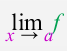
\includegraphics[scale=0.8]{tutorials/figures/palettelimit.png}
\index{limit}
\caption{You can find a shortcut for limits in the palettes toolbar under Calculus.}
\end{marginfigure}

\section{One-Sided Limits}

For one-sided limits, you will need to add an additional parameter to the \texttt{limit()} command, specifying which side (left or right) to approach the value from. In the case of a vertical asymptote, these limits will be equal to $\pm \infty$.

\begin{maplegroup}
\begin{mapleinput}
\mapleinline{active}{1d}{L(x) := 1/x;
}{}
\end{mapleinput}
\mapleresult
\begin{maplelatex}
\mapleinline{inert}{2d}{L := proc (x) options operator, arrow; 1/x end proc}{\[\displaystyle L\, := \,x\mapsto {x}^{-1}\]}
\end{maplelatex}
\end{maplegroup}

\marginnote[0.5cm]{Some versions of Maple may not properly display graphs of functions that contain vertical asymptotes. Include \texttt{discont=true} as a parameter in the \texttt{plot( )} command when required. \index{plot!discontinuities}}
\begin{maplegroup}
\begin{mapleinput}
\mapleinline{active}{1d}{plot(L(x), x=-3..3, y=-5..5);
}{}
\end{mapleinput}
\mapleresult
\mapleplot{tutorials/figures/Limitsplot2d1-eps-converted-to.pdf}
\end{maplegroup}

\begin{maplegroup}
\begin{mapleinput}
\mapleinline{active}{1d}{limit(L(x), x=0, right);
}{}
\index{limit!one-sided}
\end{mapleinput}
\mapleresult
\begin{maplelatex}
\mapleinline{inert}{2d}{infinity}{\[\displaystyle \infty \]}
\end{maplelatex}
\end{maplegroup}

\begin{maplegroup}
\begin{mapleinput}
\mapleinline{active}{1d}{limit(L(x), x=0, left);
}{}
\index{limit!one-sided}
\end{mapleinput}
\mapleresult
\begin{maplelatex}
\mapleinline{inert}{2d}{-infinity}{\[\displaystyle -\infty \]}
\end{maplelatex}
\end{maplegroup}

\begin{maplegroup}
\begin{mapleinput}
\mapleinline{active}{2d}{}{\[\]}
\end{mapleinput}
\end{maplegroup}

\subsection{Vertical Asymptotes and One-Sided Limits}
\label{subsec:vertical_asymptotes}

In this example, we will examine a rational function and use limits to determine its vertical asymptotes.

\begin{maplegroup}
\begin{mapleinput}
\mapleinline{active}{1d}{f(x) := (x\symbol{94}2-x-6)/(x\symbol{94}2-8*x+15);
}{}
\end{mapleinput}
\mapleresult
\begin{maplelatex}
\mapleinline{inert}{2d}{f := proc (x) options operator, arrow; (x^2-x-6)/(x^2-8*x+15) end proc}{\[\displaystyle f\, := \,x\mapsto {\frac {{x}^{2}-x-6}{{x}^{2}-8\,x+15}}\]}
\end{maplelatex}
\end{maplegroup}

\noindent
We can factor the denominator to find the domain of $f(x)$ and predict where we might find vertical asymptotes.

\marginnote{There is a useful \texttt{denom()}\index{mathematical functions!denominator} command that Maple provides. You can type \texttt{denom(f(x))} to get the denominator of $f(x)$.}
\begin{maplegroup}
\begin{mapleinput}
\mapleinline{active}{1d}{factor(x\symbol{94}2-8*x+15);
}{}
\end{mapleinput}
\mapleresult
\begin{maplelatex}
\mapleinline{inert}{2d}{(x-3)*(x-5)}{\[\displaystyle  \left( x-3 \right)  \left( x-5 \right) \]}
\end{maplelatex}
\end{maplegroup}

\noindent
It looks like $x=3$ and $x=5$ are not in the domain of $f(x)$. We can find the limit of $f(x)$ as $x \rightarrow 3$.

\begin{maplegroup}
\begin{mapleinput}
\mapleinline{active}{1d}{limit(f(x), x=3);
}{}
\end{mapleinput}
\mapleresult
\begin{maplelatex}
\mapleinline{inert}{2d}{-5/2}{\[\displaystyle -5/2\]}
\end{maplelatex}
\end{maplegroup}

\noindent
Since this limit exists but $f(3)$ does not, this is a \textit{removable discontinuity} and not a vertical asymptote. Now we can find the limit of $f(x)$ as $x \rightarrow 5$.

\begin{maplegroup}
\begin{mapleinput}
\mapleinline{active}{1d}{limit(f(x), x=5);
}{}
\end{mapleinput}
\mapleresult
\begin{maplelatex}
\mapleinline{inert}{2d}{undefined}{\[\displaystyle {\it undefined}\]}
\end{maplelatex}
\end{maplegroup}

\noindent
Even though this limit does not exist, we cannot automatically conclude that $f(x)$ has a vertical asymptote at $x=5$. We need to compute the one-sided limits to see if there is asymptotic behaviour.

\marginnote{Maple provides an \texttt{Asymptotes()} command that you can investigate using Maple help. Try typing \texttt{?Asymptotes} to learn more.}
\begin{maplegroup}
\begin{mapleinput}
\mapleinline{active}{1d}{limit(f(x), x=5, left);
}{}
\end{mapleinput}
\begin{mapleinput}
\mapleinline{active}{1d}{limit(f(x), x=5, right);
}{}
\end{mapleinput}
\mapleresult
\begin{maplelatex}
\mapleinline{inert}{2d}{-infinity}{\[\displaystyle -\infty \]}
\end{maplelatex}
\mapleresult
\begin{maplelatex}
\mapleinline{inert}{2d}{infinity}{\[\displaystyle \infty \]}
\end{maplelatex}
\end{maplegroup}

\noindent
Since these limits are given as $\pm \infty$, we know that $f(x)$ has a vertical asymptote at $x=5$.

\section{Limits at Infinity}

To take the limit of a function as $x$ becomes infinitely large, Maple recognizes \texttt{infinity} and \texttt{-infinity}. These can be used to find horizontal asymptotes. If the function does not have a horizontal asymptote, the limit may result in $\pm \infty$.

\begin{maplegroup}
\begin{mapleinput}
\mapleinline{active}{1d}{g(x) := (3*x\symbol{94}2 + 5*x - 10) / (5*x\symbol{94}2 - 20*x + 1);
}{}
\end{mapleinput}
\mapleresult
\begin{maplelatex}
\mapleinline{inert}{2d}{g := proc (x) options operator, arrow; (3*x^2+5*x-10)/(5*x^2-20*x+1) end proc}{\[\displaystyle g\, := \,x\mapsto {\frac {3\,{x}^{2}+5\,x-10}{5\,{x}^{2}-20\,x+1}}\]}
\end{maplelatex}
\end{maplegroup}
\index{limit!at infinity}
\begin{maplegroup}
\begin{mapleinput}
\mapleinline{active}{1d}{limit(g(x), x=infinity);
}{}
\end{mapleinput}
\mapleresult
\begin{maplelatex}
\mapleinline{inert}{2d}{3/5}{\[\displaystyle 3/5\]}
\end{maplelatex}
\end{maplegroup}

\begin{maplegroup}
\begin{mapleinput}
\mapleinline{active}{2d}{}{\[\]}
\end{mapleinput}
\end{maplegroup}

An oscillating function such as $\sin(x)$ may not have a definable limit. Maple will attempt to determine a range for the minimum and maximum of the function.

\begin{maplegroup}
\begin{mapleinput}
\mapleinline{active}{1d}{h(x) := sin(x);
}{}
\end{mapleinput}
\mapleresult
\begin{maplelatex}
\mapleinline{inert}{2d}{h := proc (x) options operator, arrow; sin(x) end proc}{\[\displaystyle h\, := \,x\mapsto \sin \left( x \right) \]}
\end{maplelatex}
\end{maplegroup}

\marginnote{Since $\sin(x)$ oscillates between $-1$ and $1$, Maple cannot determine a unique value for the limit as $x \rightarrow -\infty$.}
\begin{maplegroup}
\begin{mapleinput}
\mapleinline{active}{1d}{limit(h(x), x=-infinity);
}{}
\index{limit!at infinity}
\end{mapleinput}
\mapleresult
\begin{maplelatex}
\mapleinline{inert}{2d}{-1 .. 1}{\[\displaystyle {-1\ldots 1}\]}
\end{maplelatex}
\end{maplegroup}

\subsection{Horizontal Asymptotes and Limits at Infinity}
\label{subsec:horizontal_asymptotes}

In this example, we will examine the function
\[ f(t) = \frac{2000}{1+{\rm e}^{-t+2}}, \]
which is known as a logistic function.
\index{mathematical functions!logistic function}
\index{mathematical functions!exponential function}
\index{plot}
\begin{maplegroup}
\begin{mapleinput}
\mapleinline{active}{1d}{logistic(t) := 2000/(1 + exp(-t+2));
}{}
\end{mapleinput}
\mapleresult
\begin{maplelatex}
\mapleinline{inert}{2d}{logistic := proc (t) options operator, arrow; 2000/(1+exp(-t+2)) end proc}{\[\displaystyle {\it logistic}\, := \,t\mapsto \frac{2000}{1+{{\rm e}^{-t+2}}}\]}
\end{maplelatex}
\end{maplegroup}

\noindent
Judging by the plot of the logistic function, it appears that the function may have horizontal asymptotes.

\marginnote{Logistic functions have many applications, such as population modeling.}
\begin{maplegroup}
\begin{mapleinput}
\mapleinline{active}{1d}{plot(logistic(t));}{}
\end{mapleinput}
\mapleresult
\mapleplot{tutorials/figures/logisticasymptotesplot2d1-eps-converted-to.pdf}
\end{maplegroup}

To find the right-hand asymptote, we take the limit as $t \rightarrow \infty$.
\marginnote{Here we are using \texttt{t=infinity} rather than $x$, since the variable of this function is $t$.}

\begin{maplegroup}
\begin{mapleinput}
\mapleinline{active}{1d}{limit(logistic(t), t=infinity);
}{}
\end{mapleinput}
\mapleresult
\begin{maplelatex}
\mapleinline{inert}{2d}{2000}{\[\displaystyle 2000\]}
\end{maplelatex}
\end{maplegroup}

To find the left-hand asymptote, we take the limit as $t \rightarrow -\infty$.

\begin{maplegroup}
\begin{mapleinput}
\mapleinline{active}{1d}{limit(logistic(t), t=-infinity);
}{}
\end{mapleinput}
\mapleresult
\begin{maplelatex}
\mapleinline{inert}{2d}{0}{\[\displaystyle 0\]}
\end{maplelatex}
\end{maplegroup}

\section{Limits and Piecewise Functions}
\label{sec:limits_and_piecewise_functions}
A piecewise function is a good opportunity to practice plotting discontinuities and investigating one- and two-sided limits.
\index{mathematical functions!piecewise}
\begin{maplegroup}
\begin{mapleinput}
\mapleinline{active}{1d}{P(x) := piecewise(x<=-1, x\symbol{94}2, x<=1, -x, 1<x, x-4);
}{}
\end{mapleinput}
\mapleresult
\begin{maplelatex}
\mapleinline{inert}{2d}{P := proc (x) options operator, arrow; piecewise(x <= -1, x^2, x <= 1, -x, 1 < x, x-4) end proc}{\[\displaystyle P\, := \,x\mapsto \begin{cases}{x}^{2}&x\leq -1 \\ -x&x\leq 1 \\ x-4&1<x\end{cases}\]}
\end{maplelatex}
\end{maplegroup}

\begin{maplegroup}
\begin{mapleinput}
\mapleinline{active}{1d}{P(x);
}{}
\end{mapleinput}
\mapleresult
\begin{maplelatex}
\mapleinline{inert}{2d}{piecewise(x <= -1, x^2, x <= 1, -x, 1 < x, x-4)}{\[\displaystyle \begin{cases}{x}^{2}& x\leq -1 \\ -x& x\leq 1 \\ x-4&1<x\end{cases}\]}
\end{maplelatex}
\end{maplegroup}
\marginnote[.3cm]{It is necessary to include the \texttt{discont=true} parameter in the \texttt{plot(~)} command here so that the jump discontinuity is properly displayed in the graph of this piecewise function.}
\marginnote[1cm]{Unfortunately, even with the \texttt{discont=true} option, Maple does not include an open dot at $(1,-3)$.}
\begin{maplegroup}
\begin{mapleinput}
\mapleinline{active}{1d}{plot(P(x), x=-4..4, y=-5..5, discont=true);
}{}
\end{mapleinput}
\mapleresult
\mapleplot{tutorials/figures/Limitsplot2d2-eps-converted-to.pdf}
\end{maplegroup}
\index{plot}
 \index{plot!discontinuities}
\index{limit}
\index{limit!one-sided}
\begin{maplegroup}
\begin{mapleinput}
\mapleinline{active}{1d}{limit(P(x), x=1);
}{}
\end{mapleinput}
\mapleresult
\begin{maplelatex}
\mapleinline{inert}{2d}{undefined}{\[\displaystyle {\it undefined}\]}
\end{maplelatex}
\end{maplegroup}

\begin{maplegroup}
\begin{mapleinput}
\mapleinline{active}{1d}{limit(P(x), x=1, left);
}{}
\end{mapleinput}
\mapleresult
\begin{maplelatex}
\mapleinline{inert}{2d}{-1}{\[\displaystyle -1\]}
\end{maplelatex}
\end{maplegroup}

\begin{maplegroup}
\begin{mapleinput}
\mapleinline{active}{1d}{limit(P(x), x=1, right);
}{}
\end{mapleinput}
\mapleresult
\begin{maplelatex}
\mapleinline{inert}{2d}{-3}{\[\displaystyle -3\]}
\end{maplelatex}
\end{maplegroup}

\section{The Limit Methods Tutor}\index{limit!tutor}
\label{sec:limitmethodstutor}

The Limit Methods tutor will walk you through each step needed to evaluate a limit, including all of the limit laws learned in class. The tutor will open in a new interactive window and will output all steps in your Maple worksheet once the window is closed.

\begin{figure}[h]
\caption{Opening up the Limit Methods tutor using menus.}
\centering
\adjincludegraphics[width=\textwidth]{tutorials/figures/LimitTutorLoad-eps-converted-to.pdf}
\end{figure}

\begin{figure}[h]
\caption{Opening up the Limit Methods tutor using commands. The \texttt{Student[Calculus1]} package is required.}
\centering
\adjincludegraphics[width=\textwidth]{tutorials/figures/LimitTutorLoad2-eps-converted-to.pdf}
\end{figure}

\newpage

\subsection{Using Limit Laws for a One-sided Limit}
\index{limit!tutor!one-sided}
This example will illustrate all of the steps required to evaluate \[ \displaystyle\lim_{x \rightarrow 2^+} \frac{x-2}{x^2-x-2}. \]
\begin{figure}[h]
\caption{Begin by typing out the function, the variable name, and the value that you want the variable to approach. The direction can be specified in the drop down menu to the right of the variable information. Hit Start. You can click on individual limit laws to see whether they apply to the given limit.}
\centering
\adjincludegraphics[width=0.9\textwidth,trim={0 {0.2\height} 0 0},clip]{tutorials/figures/LimitTutorQ1-1-eps-converted-to.pdf}
\vspace{-1cm}
\end{figure}
\marginnote[-2.9cm]{When typing out the function in the tutor, you will not have access to the palettes toolbar in Maple. You will need to type out commands such as \texttt{sqrt()} for square roots. You must also include the symbol * for multiplication.}

\begin{figure}[h]
\caption{You can press the Next Step or All Steps buttons to have Maple show you a step-by-step solution.}
\centering
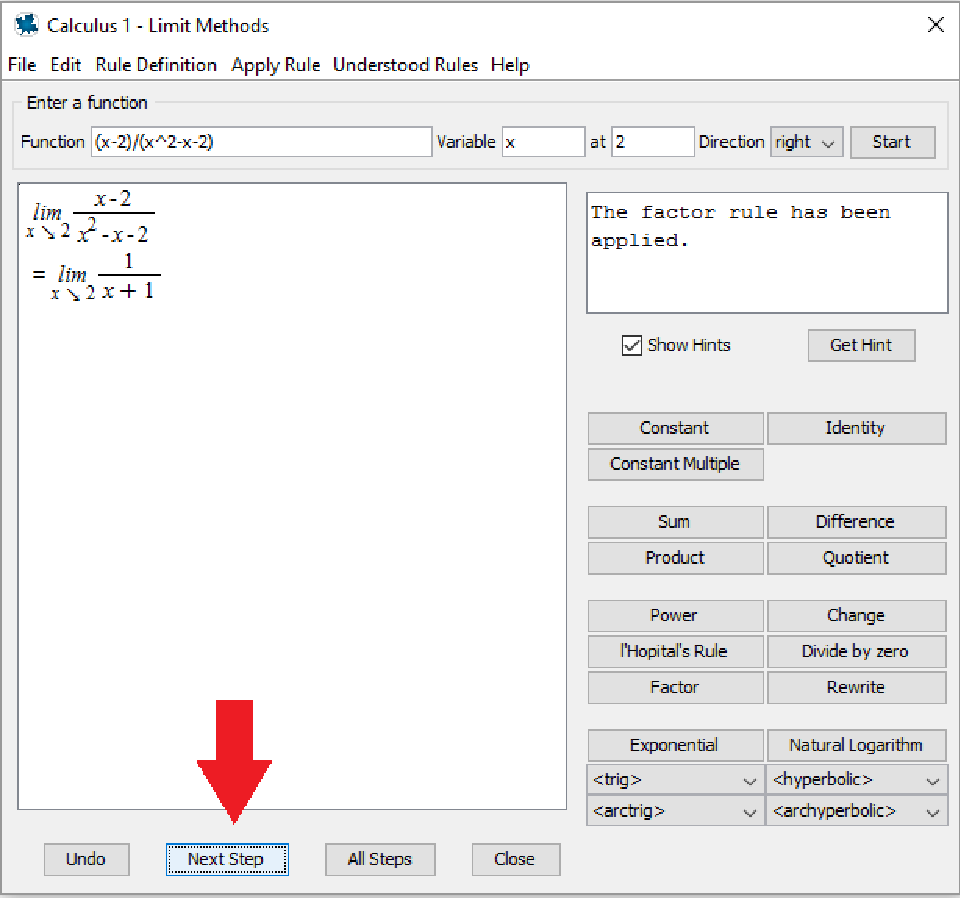
\includegraphics[width=0.9\textwidth]{tutorials/figures/LimitTutorQ1-2-eps-converted-to.pdf}
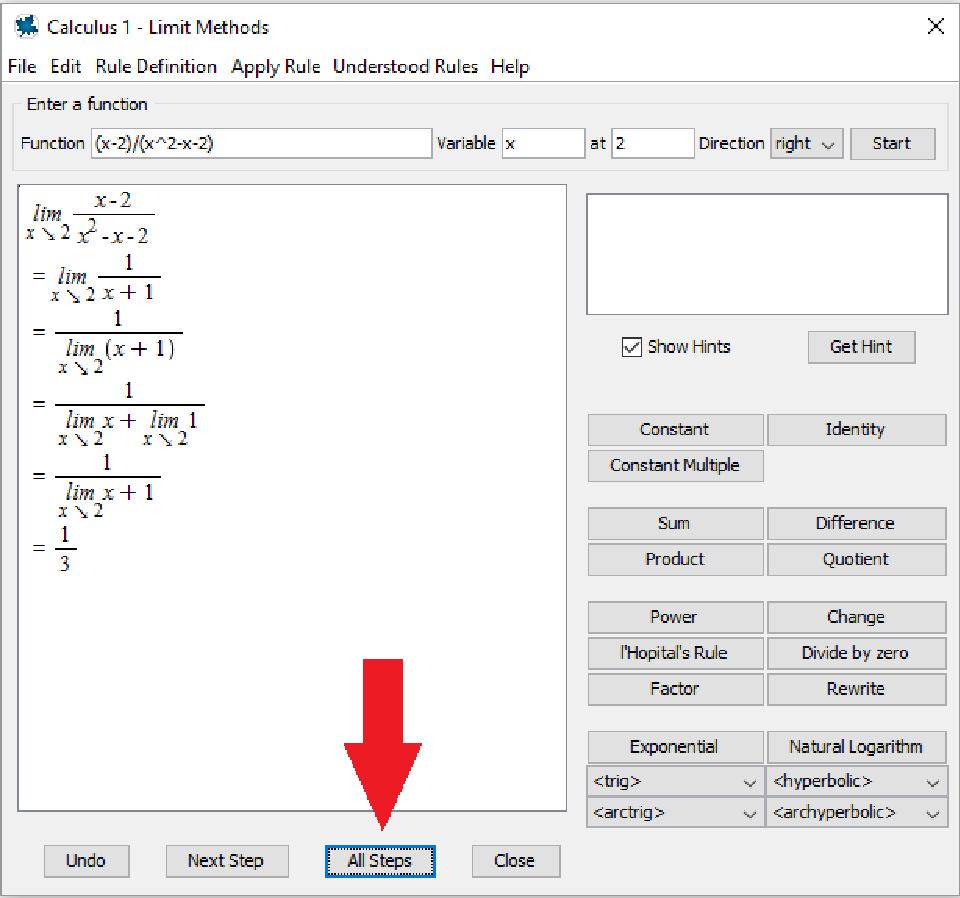
\includegraphics[width=0.9\textwidth]{tutorials/figures/LimitTutorQ1-3-eps-converted-to.pdf}
\end{figure}
\newpage

\clearpage

\subsection{Using Limit Laws for a Limit at Infinity}
\index{limit!tutor!at infinity}
In this example, we will see all of the limit laws used to evaluate \[ \displaystyle\lim_{x \rightarrow -\infty} \frac{2x-1}{\sqrt{x^2-x+3}}. \]

\begin{figure}[h]
\caption{For a limit as $x \rightarrow \infty$ or $x \rightarrow -\infty$, Maple recognizes the word \texttt{infinity}.}
\centering
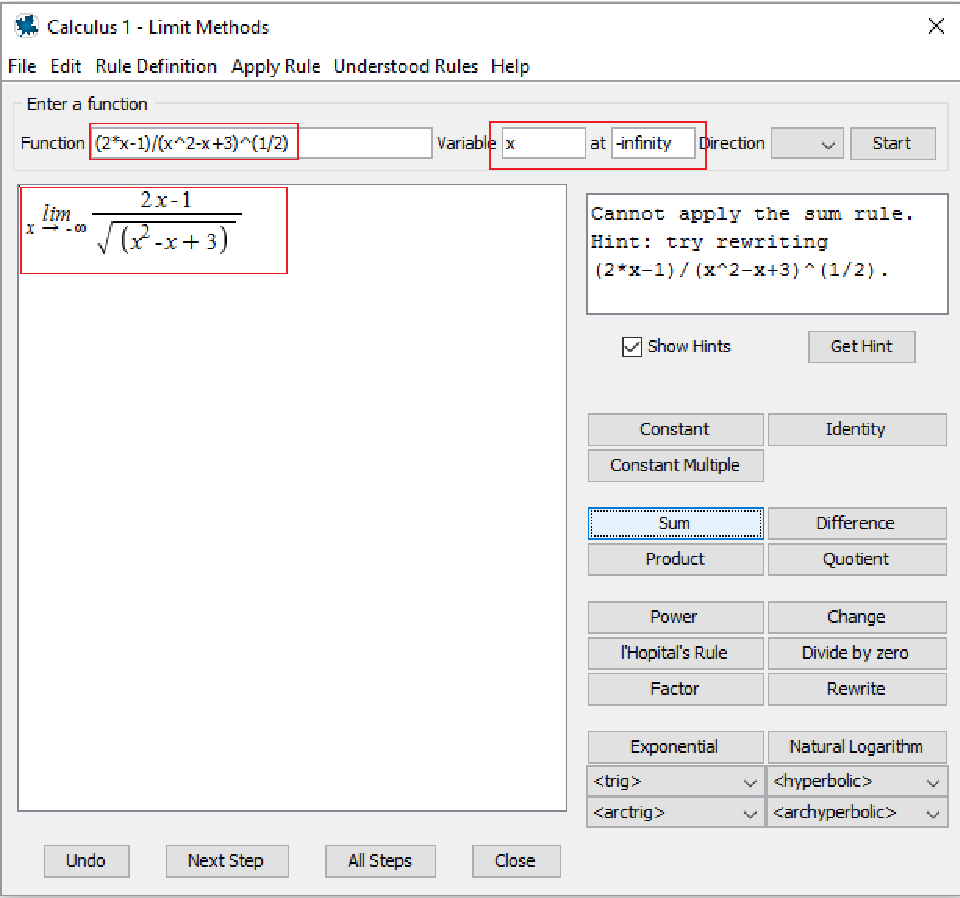
\includegraphics[width=\textwidth]{tutorials/figures/LimitTutorQ2-1-eps-converted-to.pdf}
\end{figure}
\marginnote[-3cm]{An alternate method for inputting the function into the tutor involves the \texttt{sqrt()} command.}

\begin{figure}[h]
\caption{You can click the Next Step or All Steps buttons to have Maple show you a step-by-step solution.}
\centering
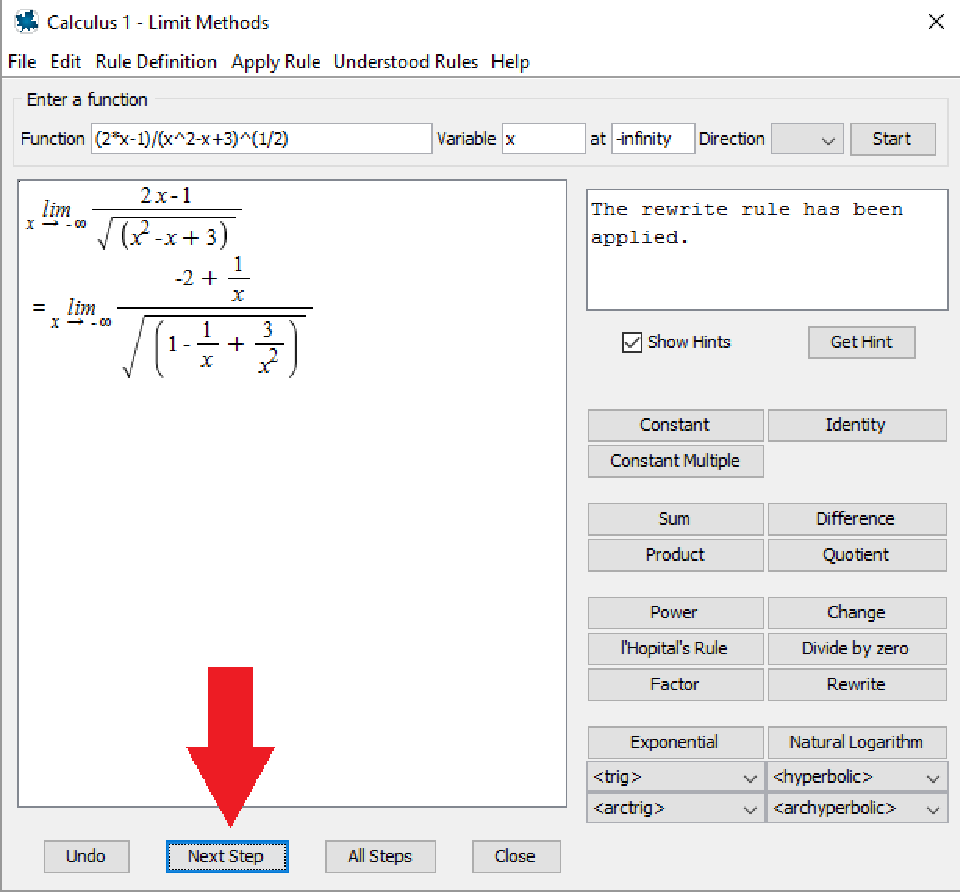
\includegraphics[width=\textwidth]{tutorials/figures/LimitTutorQ2-2-eps-converted-to.pdf}
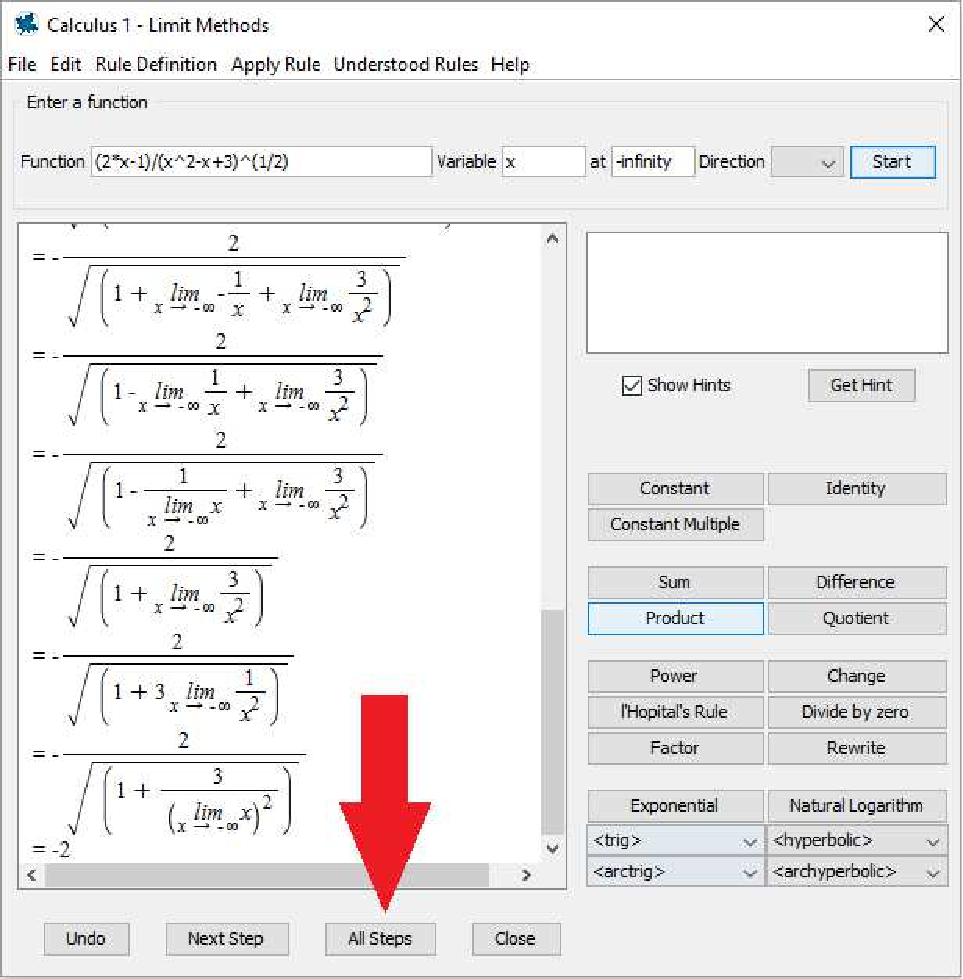
\includegraphics[width=\textwidth]{tutorials/figures/LimitTutorQ2-3-eps-converted-to.pdf}
\end{figure}
\chapter{The Derivative}
\label{chp:derivative}			

\section{The \texttt{diff()} Command}

The \texttt{diff()} command is probably the most basic way of finding the derivative of an expression. The first parameter is the expression to be differentiated and the second parameter is the variable that the expression is to be differentiated with respect to.
\index{derivative!diff}
\index{mathematical functions!inverse tangent}
\index{mathematical functions!sine}
\index{subs}
\index{simplify}
\index{ditto operator}
\index{Pi}
\begin{maplegroup}
\begin{mapleinput}
\mapleinline{active}{1d}{diff(arctan(t), t);
}{}
\end{mapleinput}
\mapleresult
\begin{maplelatex}
\mapleinline{inert}{2d}{1/(t^2+1)}{\[\displaystyle  \frac{1}{{t}^{2}+1}\]}
\end{maplelatex}
\end{maplegroup}

If you have assigned a function, then make sure to use proper function notation inside the \texttt{diff()} command.

\begin{maplegroup}
\begin{mapleinput}
\mapleinline{active}{1d}{f(x) := sin(x);
}{}
\end{mapleinput}
\mapleresult
\begin{maplelatex}
\mapleinline{inert}{2d}{f := proc (x) options operator, arrow; sin(x) end proc}{\[\displaystyle f\, := \,x\mapsto \sin \left( x \right) \]}
\end{maplelatex}
\end{maplegroup}

\marginnote{Make sure that you are taking the derivative with respect to the desired variable.}
\begin{maplegroup}
\begin{mapleinput}
\mapleinline{active}{1d}{deriv1 := diff(f(x), x);
}{}
\end{mapleinput}
\mapleresult
\begin{maplelatex}
\mapleinline{inert}{2d}{deriv1 := cos(x)}{\[\displaystyle {\it deriv1}\, := \,\cos \left( x \right) \]}
\end{maplelatex}
\end{maplegroup}

\begin{maplegroup}
\begin{mapleinput}
\mapleinline{active}{1d}{slope := subs(x = Pi/2, deriv1); simplify(%);
}{}
\end{mapleinput}
\mapleresult
\begin{maplelatex}
\mapleinline{inert}{2d}{slope := cos((1/2)*Pi)}{\[\displaystyle {\it slope}\, := \,\cos \left( \pi/2 \right) \]}
\end{maplelatex}
\mapleresult
\begin{maplelatex}
\mapleinline{inert}{2d}{0.}{\[\displaystyle  0\]}
\end{maplelatex}
\end{maplegroup}

\subsection{Higher Derivatives using \texttt{diff()}}

Higher derivatives can be evaluated by applying the \texttt{diff()} command multiple times, by specifying the variable repetitively, or using the \$ notation, as shown below.
\index{derivative!diff!higher derivatives}
\begin{maplegroup}
\begin{mapleinput}
\mapleinline{active}{1d}{diff(arctan(t), t); diff(%,t); 
}{}
\end{mapleinput}
\mapleresult
\begin{maplelatex}
\mapleinline{inert}{2d}{1/(t^2+1)}{\[\displaystyle  \frac{1}{{t}^{2}+1}\]}
\end{maplelatex}
\mapleresult
\begin{maplelatex}
\mapleinline{inert}{2d}{-2*t/(t^2+1)^2}{\[\displaystyle -\,{\frac {2t}{ \left( {t}^{2}+1 \right) ^{2}}}\]}
\end{maplelatex}
\end{maplegroup}

\begin{maplegroup}
\begin{mapleinput}
\mapleinline{active}{1d}{diff(f(x), x, x);
}{}
\end{mapleinput}
\mapleresult
\begin{maplelatex}
\mapleinline{inert}{2d}{-sin(x)}{\[\displaystyle -\sin \left( x \right) \]}
\end{maplelatex}
\end{maplegroup}

\begin{marginfigure}
\centering
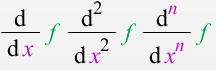
\includegraphics[scale=0.8]{tutorials/figures/palettediff.png}
\caption{You can also make use of quick shortcuts from the Calculus palette.}
\end{marginfigure}

\begin{maplegroup}
\begin{mapleinput}
\mapleinline{active}{1d}{diff(f(x), x$2);
}{}
\end{mapleinput}
\mapleresult
\begin{maplelatex}
\mapleinline{inert}{2d}{-sin(x)}{\[\displaystyle -\sin \left( x \right) \]}
\end{maplelatex}
\end{maplegroup}

\section{Using Function Notation}

If you have properly defined a function $f(x)$, you may also make use of the familiar $f'(x)$ notation used in class.
\index{derivative!prime notation}
\index{mathematical functions!sine}
\index{Pi}
\begin{maplegroup}
\begin{mapleinput}
\mapleinline{active}{1d}{f(x) := sin(x) + x\symbol{94}2;
}{}
\end{mapleinput}
\mapleresult
\begin{maplelatex}
\mapleinline{inert}{2d}{f := proc (x) options operator, arrow; sin(x)+x^2 end proc}{\[\displaystyle f\, := \,x\mapsto \sin \left( x \right) +{x}^{2}\]}
\end{maplelatex}
\end{maplegroup}

\begin{maplegroup}
\begin{mapleinput}
\mapleinline{active}{1d}{deriv1 := f'(x);
}{}
\end{mapleinput}
\mapleresult
\begin{maplelatex}
\mapleinline{inert}{2d}{deriv1 := cos(x)+2*x}{\[\displaystyle {\it deriv1}\, := \,\cos \left( x \right) +2\,x\]}
\end{maplelatex}
\end{maplegroup}

\noindent
This notation is especially useful for evaluating the derivative at a value, without using the \texttt{subs()} command separately.

\begin{maplegroup}
\begin{mapleinput}
\mapleinline{active}{1d}{slope1 := f'(0);
}{}
\end{mapleinput}
\mapleresult
\begin{maplelatex}
\mapleinline{inert}{2d}{1}{\[\displaystyle {\it deriv1}\, := \, 1\]}
\end{maplelatex}
\end{maplegroup}

\marginnote{While using $m$ is a common choice for slope, it is a good idea to avoid overusing it in your Maple worksheet.}
\begin{maplegroup}
\begin{mapleinput}
\mapleinline{active}{1d}{slope2 := f'(Pi);
}{}
\end{mapleinput}
\mapleresult
\begin{maplelatex}
\mapleinline{inert}{2d}{1}{\[\displaystyle {\it slope2}\, := \, -1 + 2\pi\]}
\end{maplelatex}
\end{maplegroup}


\subsection{Higher Derivatives using Prime Notation}

Higher derivatives are also notated in much the same way as in class. Rather than using a string of tick marks, we use a raised exponent in parentheses to specify the $n$\textsuperscript{th} derivative.
\index{derivative!prime notation!higher derivatives}
\begin{maplegroup}
\begin{mapleinput}
\mapleinline{active}{1d}{deriv2 := f''(x);
}{}
\end{mapleinput}
\mapleresult
\begin{maplelatex}
\mapleinline{inert}{2d}{deriv2 := -sin(x)+2}{\[\displaystyle {\it deriv2}\, := -\sin \left( x \right) +2\]}
\end{maplelatex}
\end{maplegroup}

\begin{maplegroup}
\begin{mapleinput}
\mapleinline{active}{1d}{deriv3 := f\textsuperscript{(3)}(x);
}{}
\end{mapleinput}
\mapleresult
\begin{maplelatex}
\mapleinline{inert}{2d}{deriv3 := -cos(x)}{\[\displaystyle {\it deriv3}\, := -\cos \left( x \right)\]}
\end{maplelatex}
\end{maplegroup}

\section{Applications of the Derivative}

In these examples, we will use the function notation method for derivatives, though the \texttt{diff()} command may also be used.

\subsection{Finding the Equation of a Tangent Line}
\label{subsec:equation_of_tangent_line}
\index{lines!tangent line}
\index{mathematical functions!square root}
In this example, we will find the equation of the tangent line to the function $f(x)=6\sqrt{x} - 2x$ at $x=4$. We start by assigning the function a name.

\begin{maplegroup}
\begin{mapleinput}
\mapleinline{active}{1d}{f(x) := 6*sqrt(x) - 2*x;
}{}
\end{mapleinput}
\mapleresult
\begin{maplelatex}
\mapleinline{inert}{2d}{f := proc (x) options operator, arrow; 6*sqrt(x)-2*x end proc}{\[\displaystyle f\, := \,x\mapsto 6\,\sqrt {x}-2\,x\]}
\end{maplelatex}
\end{maplegroup}

\begin{maplegroup}
\begin{mapleinput}
\mapleinline{active}{1d}{f'(x);
}{}
\end{mapleinput}
\mapleresult
\begin{maplelatex}
\mapleinline{inert}{2d}{3/sqrt(x)-2}{\[\displaystyle \frac{3}{\sqrt{x}}-2\]}
\end{maplelatex}
\end{maplegroup}

The $y$-coordinate and the slope can be found by substituting $x=4$ into the function and its derivative, respectively.

\begin{maplegroup}
\begin{mapleinput}
\mapleinline{active}{1d}{f(4);
}{}
\end{mapleinput}
\mapleresult
\begin{maplelatex}
\mapleinline{inert}{2d}{4}{\[\displaystyle 4\]}
\end{maplelatex}
\end{maplegroup}

\marginnote{Sometimes Maple output can be easily simplified, such as $\sqrt{4}$ here. Alternatively, an \texttt{evalf(\%)} command would produce a decimal output.}
\begin{maplegroup}
\begin{mapleinput}
\mapleinline{active}{1d}{f'(4); simplify(%);
}{}
\end{mapleinput}
\mapleresult
\begin{maplelatex}
\mapleinline{inert}{2d}{(3/4)*sqrt(4)-2}{\[\displaystyle \frac{3}{4}\, \sqrt{4}-2\]}
\end{maplelatex}
\mapleresult
\begin{maplelatex}
\mapleinline{inert}{2d}{-1/2}{\[\displaystyle -\frac{1}{2}\]}
\end{maplelatex}
\end{maplegroup}
\index{simplify}
\index{ditto operator}
\noindent
The equation of the tangent line at $x=a$ is 
\begin{equation*}
L(x) = f'(a) (x-a) + f(a).
\end{equation*} 
In this case, the tangent line is at $x=4$.
\marginnote{The equation of a tangent line is a major topic of Math 112. Make sure you know this equation well!}

\begin{maplegroup}
\begin{mapleinput}
\mapleinline{active}{1d}{line := f'(4)*(x-4) + f(4); expand(line);
}{}
\end{mapleinput}
\mapleresult
\begin{maplelatex}
\mapleinline{inert}{2d}{line := ((3/4)*sqrt(4)-2)*(x-4)+4}{\[\displaystyle {\it line}\, := \, \left( \frac{3}{4}\, \sqrt{4}-2 \right)  \left( x-4 \right) +4\]}
\end{maplelatex}
\mapleresult
\marginnote{After expanding the equation, we have the equation of a line in standard $y=mx+b$ form.}
\begin{maplelatex}
\mapleinline{inert}{2d}{-(1/2)*x+6}{\[\displaystyle -\frac{1}{2}x+6\]}
\end{maplelatex}
\end{maplegroup}

\index{expand}
\index{plot}
\index{plot!multiple functions}
\index{plot!axes intervals}

\noindent
Notice that the line is only defined as an expression and is not in function notation. We can now plot the function and the line.

\begin{maplegroup}
\begin{mapleinput}
\mapleinline{active}{1d}{plot([f(x),line], x=-1..10);}{}
\end{mapleinput}
\mapleresult
\mapleplot{tutorials/figures/TangentLine-eps-converted-to.pdf}
\end{maplegroup}
\marginnote[-2cm]{It is a good idea to specify plot colours, especially if plotting more than one tangent line on the same axes.}

\subsection{The Closed Interval Method for Min/Max Problems}
\label{subsec:closed_interval_method}

\index{shapes of curves!maximum}
\index{shapes of curves!minimum}

\index{shapes of curves!closed interval method}

In this example, we will find the absolute minimum and maximum values of 
\begin{equation*}
\displaystyle f(x) = \frac {-x^4+5x^3+20}{\sqrt{x^2+1}}
\end{equation*}
on the interval $[-1,5]$. It is best to define the function and plot it first to get an idea of where the critical numbers are located.

\index{mathematical functions!square root}
\marginnote[2cm]{Here we have chosen to plot the function $f(x)$ on the interval $[-1.5, 5.5]$.}
\begin{maplegroup}
\begin{mapleinput}
\mapleinline{active}{1d}{f(x) := (20 + 5*x\symbol{94}3 - x\symbol{94}4)/sqrt(x\symbol{94}2 + 1);
}{}
\index{assignment operator}
\end{mapleinput}
\mapleresult
\begin{maplelatex}
\mapleinline{inert}{2d}{f := proc (x) options operator, arrow; (20+5*x^3-x^4)/sqrt(x^2+1) end proc}{\[\displaystyle f\, := \,x\mapsto {\frac {-{x}^{4}+5\,{x}^{3}+20}{\sqrt {{x}^{2}+1}}}\]}
\end{maplelatex}
\end{maplegroup}

\index{plot}
\index{plot!axes intervals}

\begin{maplegroup}
\begin{mapleinput}
\mapleinline{active}{1d}{plot(f(x), x=-1.5..5.5);
}{}
\label{Plot!plot}
\end{mapleinput}
\mapleresult
\mapleplot{tutorials/figures/ExtremeValues-eps-converted-to.pdf}
\end{maplegroup}

By factoring the derivative, we can see that $x=0$ is a critical number. We can use the \texttt{fsolve()} command over smaller intervals to find the remaining critical numbers.

\index{factor}
\index{shapes of curves!critical number}
\index{solving equations!fsolve}
\index{derivative!prime notation}
\index{solving equations!fsolve!interval}

\begin{maplegroup}
\begin{mapleinput}
\mapleinline{active}{1d}{factor(f'(x));
}{}
\end{mapleinput}
\mapleresult
\begin{maplelatex}
\mapleinline{inert}{2d}{-x*(3*x^4-10*x^3+4*x^2-15*x+20)/(x^2+1)^(3/2)}{\[\displaystyle -{\frac {x \left( 3\,{x}^{4}-10\,{x}^{3}+4\,{x}^{2}-15\,x+20 \right) }{ \left( {x}^{2}+1 \right) ^{3/2}}}\]}
\end{maplelatex}
\end{maplegroup}

\marginnote{If a closed interval was not specified, we could use the second derivative test to find local minima and maxima.
	
	\begin{maplegroup}
	\begin{mapleinput}
	\mapleinline{active}{1d}{f''(CN1); f''(CN2); f''(CN3);
	}{}
	\end{mapleinput}
	\mapleresult
	\begin{maplelatex}
	\mapleinline{inert}{2d}{-20}{\[\displaystyle -20\]}
	\end{maplelatex}
	\mapleresult
	\begin{maplelatex}
	\mapleinline{inert}{2d}{8.886020129}{\[\displaystyle  8.886020129\]}
	\end{maplelatex}
	\mapleresult
	\begin{maplelatex}
	\mapleinline{inert}{2d}{-8.221546325}{\[\displaystyle - 8.221546325\]}
	\end{maplelatex}
	\end{maplegroup}
	
	\noindent
	Since $f(x)$ is concave down at \texttt{CN1} and \texttt{CN3}, we have found two local maxima. Since $f(x)$ is concave up at \texttt{CN2}, we have found one local minimum.
}

\begin{maplegroup}
\begin{mapleinput}
\mapleinline{active}{1d}{CN1:=0;
}{}
\end{mapleinput}
\mapleresult
\begin{maplelatex}
\mapleinline{inert}{2d}{CN1 := 0}{\[\displaystyle {\it CN1}\, := \,0\]}
\end{maplelatex}
\end{maplegroup}

\begin{maplegroup}
\begin{mapleinput}
\mapleinline{active}{1d}{CN2:=fsolve(f'(x)=0, x=1..2);
}{}
\end{mapleinput}
\mapleresult
\begin{maplelatex}
\mapleinline{inert}{2d}{CN2 := 1.078091128}{\[\displaystyle {\it CN2}\, := \, 1.078091128\]}
\end{maplelatex}
\end{maplegroup}

\begin{maplegroup}
\begin{mapleinput}
\mapleinline{active}{1d}{CN3:=fsolve(f'(x)=0, x=3..4);
}{}
\end{mapleinput}
\mapleresult
\begin{maplelatex}
\mapleinline{inert}{2d}{CN3 := 3.201521345}{\[\displaystyle {\it CN3}\, := \, 3.201521345\]}
\end{maplelatex}
\end{maplegroup}

To apply the closed interval method, we must evaluate the function at all critical numbers in the interval as well as the two endpoints.

\index{shapes of curves!closed interval method}
\index{evalf}

\begin{maplegroup}
\begin{mapleinput}
\mapleinline{active}{1d}{f(CN1); f(CN2); f(CN3); 
}{}
\end{mapleinput}
\mapleresult
\begin{maplelatex}
\mapleinline{inert}{2d}{20}{\[\displaystyle 20\]}
\end{maplelatex}
\mapleresult
\begin{maplelatex}
\mapleinline{inert}{2d}{16.94310958}{\[\displaystyle  16.94310958\]}
\end{maplelatex}
\mapleresult
\begin{maplelatex}
\mapleinline{inert}{2d}{23.55848432}{\[\displaystyle  23.55848432\]}
\end{maplelatex}
\end{maplegroup}

\begin{maplegroup}
\begin{mapleinput}
\mapleinline{active}{1d}{f(-1): evalf(%);
}{}
\end{mapleinput}
\mapleresult
\begin{maplelatex}
\mapleinline{inert}{2d}{9.899494934}{\[\displaystyle  9.899494934\]}
\end{maplelatex}
\end{maplegroup}

\marginnote{The full colon \texttt{:} here hides the output of inputting the endpoint into the function. Only the output of the \texttt{evalf(\%)} command is displayed.}
\begin{maplegroup}
\begin{mapleinput}
\mapleinline{active}{1d}{f(5): evalf(%);
}{}
\end{mapleinput}
\mapleresult
\begin{maplelatex}
\mapleinline{inert}{2d}{3.922322703}{\[\displaystyle  3.922322703\]}
\end{maplelatex}
\end{maplegroup}

Comparing these values, we see that $x=3.201521345$ gives an absolute maximum of $23.55848432$ and that $x=5$ gives an absolute minimum of $3.922322703$ on the interval $[-1,5]$.

\clearpage

\section{The Derivatives Tutor}

\index{derivative!tutor}

The Derivatives tutor is a useful way for visualising the graphs of the first (and second) derivatives of a given function.

\begin{figure}[h]
\caption{Opening up the Derivatives tutor using menus.}
\centering
\adjincludegraphics[width=\textwidth]{tutorials/figures/DerivativeTutorLoad1-eps-converted-to.pdf}
\end{figure}

\begin{figure}[h]
\caption{Opening up the Derivatives tutor using commands. The \texttt{Student[Calculus1]} package is required.}
\centering
\adjincludegraphics[width=\textwidth]{tutorials/figures/DerivativeTutorLoad2-eps-converted-to.pdf}
\end{figure}

\subsection{Visualising the Derivative of $(x-1)^2\sin(x)$}

\begin{figure}[h]
\caption{The Derivatives tutor displays the given function $f(x)$ as well as its derivative(s) $f'(x)$ (and optionally $f''(x)$).}
\centering
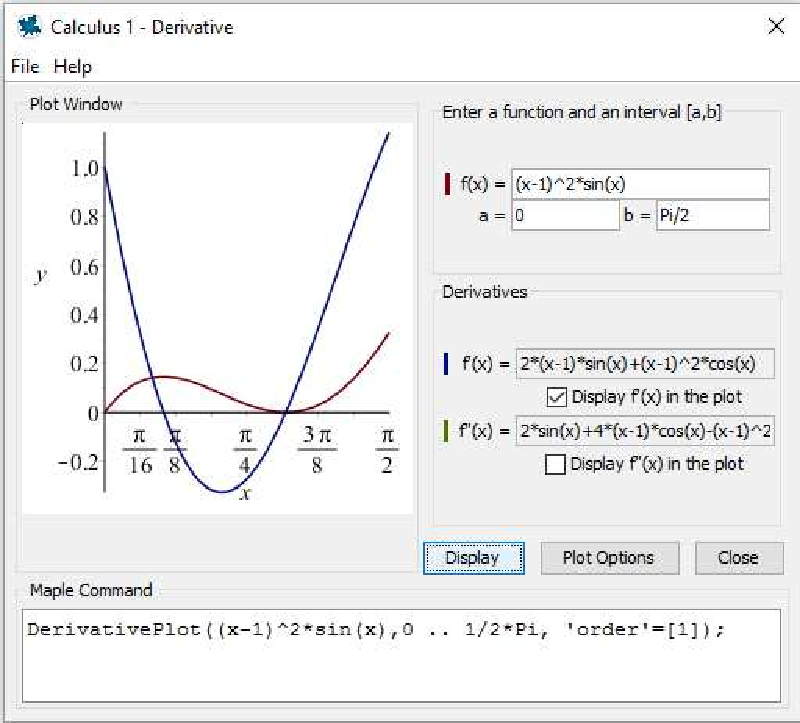
\includegraphics[width=0.8\textwidth]{tutorials/figures/DerivativeTutorQ1-1-eps-converted-to.pdf}
\vspace{-1cm}
\end{figure}
\marginnote[-4cm]{When typing out the function in the tutor, you will not have access to the palettes toolbar in Maple. You will need to type out commands such as \texttt{sqrt()} for square roots. You must also include the symbol * for multiplication.}

\begin{figure}[h]
\caption{You can optionally specify the axes ranges as well as $1:1$ scaling.}
\centering
\adjincludegraphics[width=\textwidth,trim={{0.2\width} 0 0 0},clip]{tutorials/figures/DerivativeTutorQ1-2-eps-converted-to.pdf}
\end{figure}

\section{The Differentiation Methods Tutor}

The Differentiation Methods tutor is useful for showing each individual differentiation rule as a separate step when finding the derivative of a given function.

\begin{figure}[h]
\caption{Opening up the Differentiation Methods tutor using menus.}
\centering
\adjincludegraphics[width=\textwidth]{tutorials/figures/DiffTutorLoad1-eps-converted-to.pdf}
\end{figure}

\begin{figure}[h]
\caption{Opening up the Differentiation Methods tutor using commands. The \texttt{Student[Calculus1]} package is required.}
\centering
\adjincludegraphics[width=\textwidth]{tutorials/figures/DiffTutorLoad2-eps-converted-to.pdf}
\end{figure}

\clearpage

\subsection{Differentiating $x^2\cos(x)$ using Product and Power Rules}

\begin{figure}[h]
\caption{Using the Get Hint button gives you suggestions as to what differentiation rule to use.}
\centering
\adjincludegraphics[width=0.8\textwidth,trim={0 {0.6\height} 0 0},clip]{tutorials/figures/DiffTutorQ1-1-eps-converted-to.pdf}
\adjincludegraphics[width=0.8\textwidth,trim={0 {0.3\height} 0 0},clip]{tutorials/figures/DiffTutorQ1-2-eps-converted-to.pdf}
\end{figure}

\marginnote[-4cm]{When typing out the function in the tutor, you will not have access to the palettes toolbar in Maple. You will need to type out commands such as \texttt{sqrt()} for square roots. You must also include the symbol * for multiplication.}

\begin{figure}[h]
\caption{If a rule cannot be applied, then the tutor will provide additional hints.}
\centering
\adjincludegraphics[width=0.8\textwidth,trim={0 {0.28\height} 0 0},clip]{tutorials/figures/DiffTutorQ1-3-eps-converted-to.pdf}
\end{figure}

\clearpage

\begin{figure}[h]
\caption{Using the product rule, the power rule, and the derivative of $\cos(x)$ to differentiate $x^2\cos(x)$.}
\centering
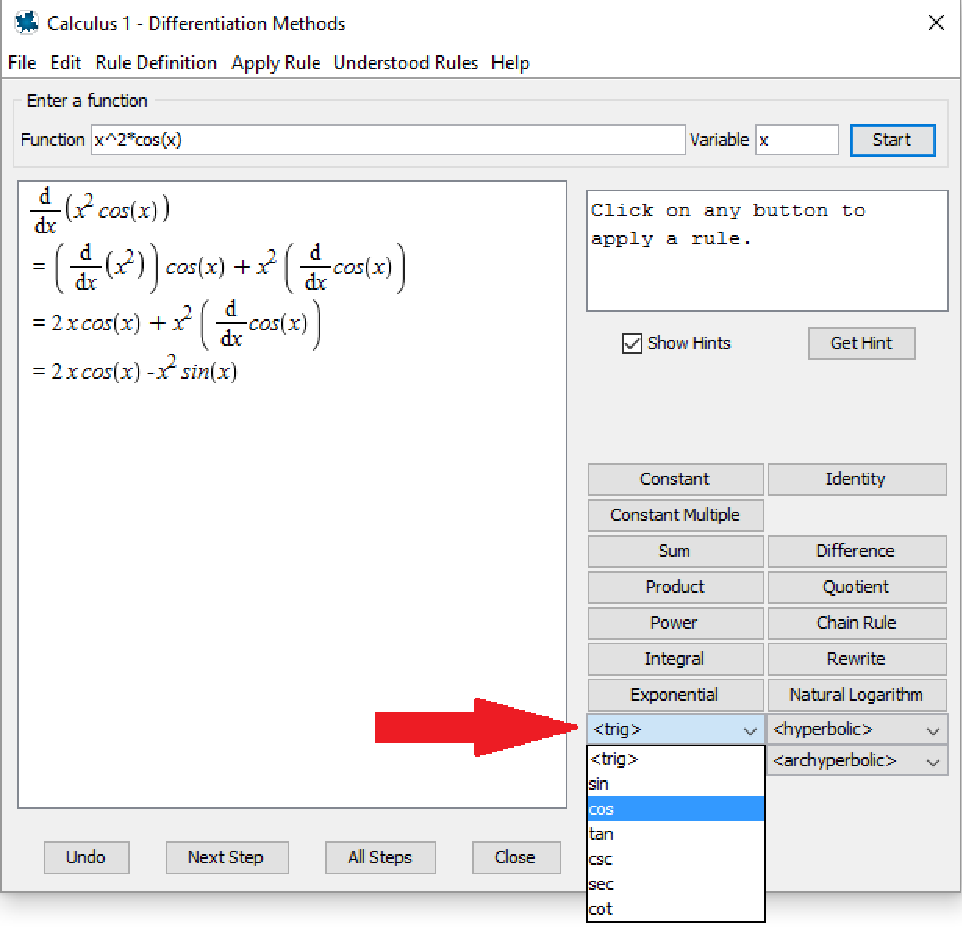
\includegraphics[width=0.8\textwidth]{tutorials/figures/DiffTutorQ1-4-eps-converted-to.pdf}\\
\end{figure}

\subsection{Differentiating $\frac{\sin(x)}{x\tan(x)}$ using Rewrite and Quotient Rule}

\begin{figure}[h]
\caption{Using the Rewrite button allows you to replace an expression with another equivalent expression.}
\centering
\adjincludegraphics[width=0.8\textwidth,trim={0 {0.2\height} 0 0},clip]{tutorials/figures/DiffTutorQ2-1-eps-converted-to.pdf}
%\adjincludegraphics[width=0.8\textwidth,trim={0 {0.7\height} 0 0},clip]{tutorials/figures/DiffTutorQ2-2-eps-converted-to.pdf}
\end{figure}

\clearpage

\begin{figure}[h]
\caption{Applying the quotient rule to differentiate $\frac{\sin(x)}{x\tan(x)}$.}
\centering
\adjincludegraphics[width=0.8\textwidth,trim={0 {0.3\height} 0 0},clip]{tutorials/figures/DiffTutorQ2-3-eps-converted-to.pdf}
\end{figure}

\section{Newton's Method} \label{sec:newtonsmethod}

Suppose we start with the function $f(x) = {\rm e}^x - 2$. We know that the root of this function is $x = \ln 2$. If we wish to evaluate $\ln 2$ as a decimal, we can simply use \texttt{fsolve()}.

\index{mathematical functions!exponential}
\index{solving equations!fsolve}

\index{packages!Student[Calculus1]}

\begin{maplegroup}
\begin{mapleinput}
\mapleinline{active}{1d}{f(x) := exp(x) - 2;
}{}
\end{mapleinput}
\mapleresult
\begin{maplelatex}
\mapleinline{inert}{2d}{f := proc (x) options operator, arrow; exp(x)-2 end proc}{\[\displaystyle f\, := \,x\mapsto {{\rm e}^{x}}-2\]}
\end{maplelatex}
\end{maplegroup}

\begin{maplegroup}
\begin{mapleinput}
\mapleinline{active}{1d}{fsolve(f(x) = 0);
}{}
\end{mapleinput}
\mapleresult
\begin{maplelatex}
\mapleinline{inert}{2d}{.6931471806}{\[\displaystyle  0.6931471806\]}
\end{maplelatex}
\end{maplegroup}

We can also find this root by applying Newton's method with an initial guess of $x=2$. We need to load the \texttt{Student[Calculus1]} package before we use the \texttt{NewtonsMethod()} command. 

Optional parameters may be included to change how the result is displayed and how many iterations of the method are performed.

\index{Newton's method!NewtonsMethod!output options}
\index{Newton's method!NewtonsMethod!iterations}

\begin{table}
\label{tbl:newtonsmethod_options}
\centering
\begin{tabular}{lp{2.5in}}
\hline
Parameter & Description\\
\hline
\texttt{output = value}			& Outputs the numerical result of Newton's method.\\
\texttt{output = plot}			& Outputs a plot showing the tangent line approximation approach to finding the root.\\
\texttt{output = animation}		& Much like the \texttt{plot} output, only with each iteration as a separate frame.\\
\texttt{output = sequence}		& Outputs the original guess and the result of each iteration of Newton's method.\\
\texttt{iterations = }$n$		& Specifies the number of iterations to perform in Newton's method.\\
\hline
\end{tabular}
\caption{A list of optional parameters for the \texttt{NewtonsMethod()} command.}
\end{table}

\clearpage

\begin{maplegroup}
\begin{mapleinput}
\mapleinline{active}{1d}{with(Student[Calculus1]):
}{}
\end{mapleinput}
\end{maplegroup}

\index{packages!with}
\index{packages!Student[Calculus1]}

\begin{maplegroup}
\begin{mapleinput}
\mapleinline{active}{1d}{NewtonsMethod(f(x), x=2, output=plot);
}{}
\end{mapleinput}
\mapleresult
\mapleplot{tutorials/figures/newtonsmethodplot2d1-eps-converted-to.pdf}
\end{maplegroup}

If we wish to simply evaluate the root, the \texttt{output=plot} option may be omitted. For more accuracy, the algorithm can be run with additional iterations.

\index{Newton's method!NewtonsMethod}

\begin{maplegroup}
\begin{mapleinput}
\mapleinline{active}{1d}{NewtonsMethod(f(x), x=2);
}{}
\end{mapleinput}
\mapleresult
\begin{maplelatex}
\mapleinline{inert}{2d}{.6931471814}{\[\displaystyle  0.6931471814\]}
\end{maplelatex}
\end{maplegroup}

\index{Newton's method!NewtonsMethod!output options}
\index{Newton's method!NewtonsMethod!iterations}

\marginnote[1cm]{The default number of iterations for \texttt{NewtonsMethod()} with the parameter \texttt{ouput=sequence} is $5$.}
\begin{maplegroup}
\begin{mapleinput}
\mapleinline{active}{1d}{NewtonsMethod(f(x), x=2, output=sequence);
}{}
\end{mapleinput}
\mapleresult
\begin{maplelatex}
\mapleinline{inert}{2d}{2, 1.270670566, .8319573035, .7023505839, .6931894021, .6931471814}{\[\displaystyle \begin{array}{l}2,\, 1.270670566,\, 0.8319573035,\, 0.7023505839,\, \\ 0.6931894021,\, 0.6931471814 \end{array}\]}
\end{maplelatex}
\end{maplegroup}

\begin{maplegroup}
\begin{mapleinput}
\mapleinline{active}{1d}{NewtonsMethod(f(x), x=2, iterations=10);
}{}
\end{mapleinput}
\mapleresult
\begin{maplelatex}
\mapleinline{inert}{2d}{.6931471804}{\[\displaystyle  0.6931471804\]}
\end{maplelatex}
\end{maplegroup}

\begin{maplegroup}
\begin{mapleinput}
\mapleinline{active}{1d}{}{}
\end{mapleinput}
\end{maplegroup}
\chapter{Implicit Functions}
\label{chp:implicit_functions}

\index{implicit functions}
\index{assignment operator!implicit function}

\section{Implicit Functions}
\label{sec:implicit_functions_tutorial}

An implicit function cannot be defined as a normal function. Instead, the curve is defined as an \textit{equation} of multiple variables. It is easiest to assign a name to the entire equation, including the $=$ sign.

\begin{maplegroup}
\begin{mapleinput}
\mapleinline{active}{1d}{E := y\symbol{94}2 = x\symbol{94}3 - 2*x + 1;
}{}
\end{mapleinput}
\mapleresult
\begin{maplelatex}
\mapleinline{inert}{2d}{E := y^2 = x^3-2*x+1}{\[\displaystyle E\, := \,{y}^{2}={x}^{3}-2\,x+1\]}
\end{maplelatex}
\end{maplegroup}

\index{subs}
\index{solving equations!solve}
\index{ditto operator}

\noindent
To find points on the curve, we can substitute a value for $x$ and solve for $y$.

\begin{maplegroup}
\begin{mapleinput}
\mapleinline{active}{1d}{subs(x=2, E);
}{}
\end{mapleinput}
\mapleresult
\begin{maplelatex}
\mapleinline{inert}{2d}{y^2 = 5}{\[\displaystyle {y}^{2}=5\]}
\end{maplelatex}
\end{maplegroup}

\begin{maplegroup}
\begin{mapleinput}
\mapleinline{active}{1d}{solve(%, y);
}{}
\end{mapleinput}
\mapleresult
\begin{maplelatex}
\mapleinline{inert}{2d}{sqrt(5), -sqrt(5)}{\[\displaystyle  \sqrt{5},\,- \sqrt{5}\]}
\end{maplelatex}
\end{maplegroup}

Many implicit functions cannot be expressed as a single function $y=f(x)$. However, it may be possible to split up implicit functions into explicit functions by solving for $y$.

\index{mathematical functions!nth root@$n$\textsuperscript{th} root}

\begin{maplegroup}
\begin{mapleinput}
\mapleinline{active}{1d}{L := x\symbol{94}2 + (y - root[3](x\symbol{94}2))\symbol{94}2 = 1;
}{}
\end{mapleinput}
\mapleresult
\begin{maplelatex}
\mapleinline{inert}{2d}{L := x^2+(y-(x^2)^(1/3))^2 = 1}{\[\displaystyle L\, := \,{x}^{2}+ \left( y-\sqrt [3]{{x}^{2}} \right) ^{2}=1\]}
\end{maplelatex}
\end{maplegroup}

\marginnote[-1cm]{Here, the command \texttt{root[3]()} is equivalent to $\sqrt[3]{(~)}$.}

\begin{maplegroup}
\begin{mapleinput}
\mapleinline{active}{1d}{solve(L, y);
}{}
\end{mapleinput}
\mapleresult
\begin{maplelatex}
\mapleinline{inert}{2d}{(x^2)^(1/3)+sqrt(-x^2+1), (x^2)^(1/3)-sqrt(-x^2+1)}{\[\displaystyle \sqrt [3]{{x}^{2}}+ \sqrt{-{x}^{2}+1},\,\sqrt [3]{{x}^{2}}- \sqrt{-{x}^{2}+1}\]}
\end{maplelatex}
\end{maplegroup}

\section{Plotting Implicit Functions}
\label{sec:plotting_implicit_functions}

The \texttt{implicitplot()} command can be used to plot implicit functions. It requires use of the \texttt{plots} package. Unlike the normal \texttt{plot()} command, each curve that is being plotted must be in the form of an \textit{equation} of two variables, including the $=$ sign. Additionally, you must specify an interval for \textit{both} variables.
\marginnote[.6cm]{The \texttt{plots} package can be loaded using the \texttt{with()} command. This only needs to be loaded once per Maple worksheet and needs to be run each time you open a new or previously closed document.}
\index{packages!with}
\index{packages!plots}

\begin{maplegroup}
\begin{mapleinput}
\mapleinline{active}{1d}{with(plots):
}{}
\end{mapleinput}
\end{maplegroup}

\begin{maplegroup}
\begin{mapleinput}
\mapleinline{active}{1d}{implicitplot(E, x=-5..5, y=-5..5);
}{}\index{implicit functions!implicitplot!changing axes}
\end{mapleinput}
\mapleresult
\mapleplot{tutorials/figures/Implicit_Functions_and_Graphsplot2d2-eps-converted-to.pdf}
\end{maplegroup}

Most of the implicit functions used in this lab manual will produce smooth curves when plotted. See Figure \ref{fig:plotresolution} if your plot appears to have jagged edges.
\begin{marginfigure}
\index{implicit functions!implicitplot!plot resolution}
\centering
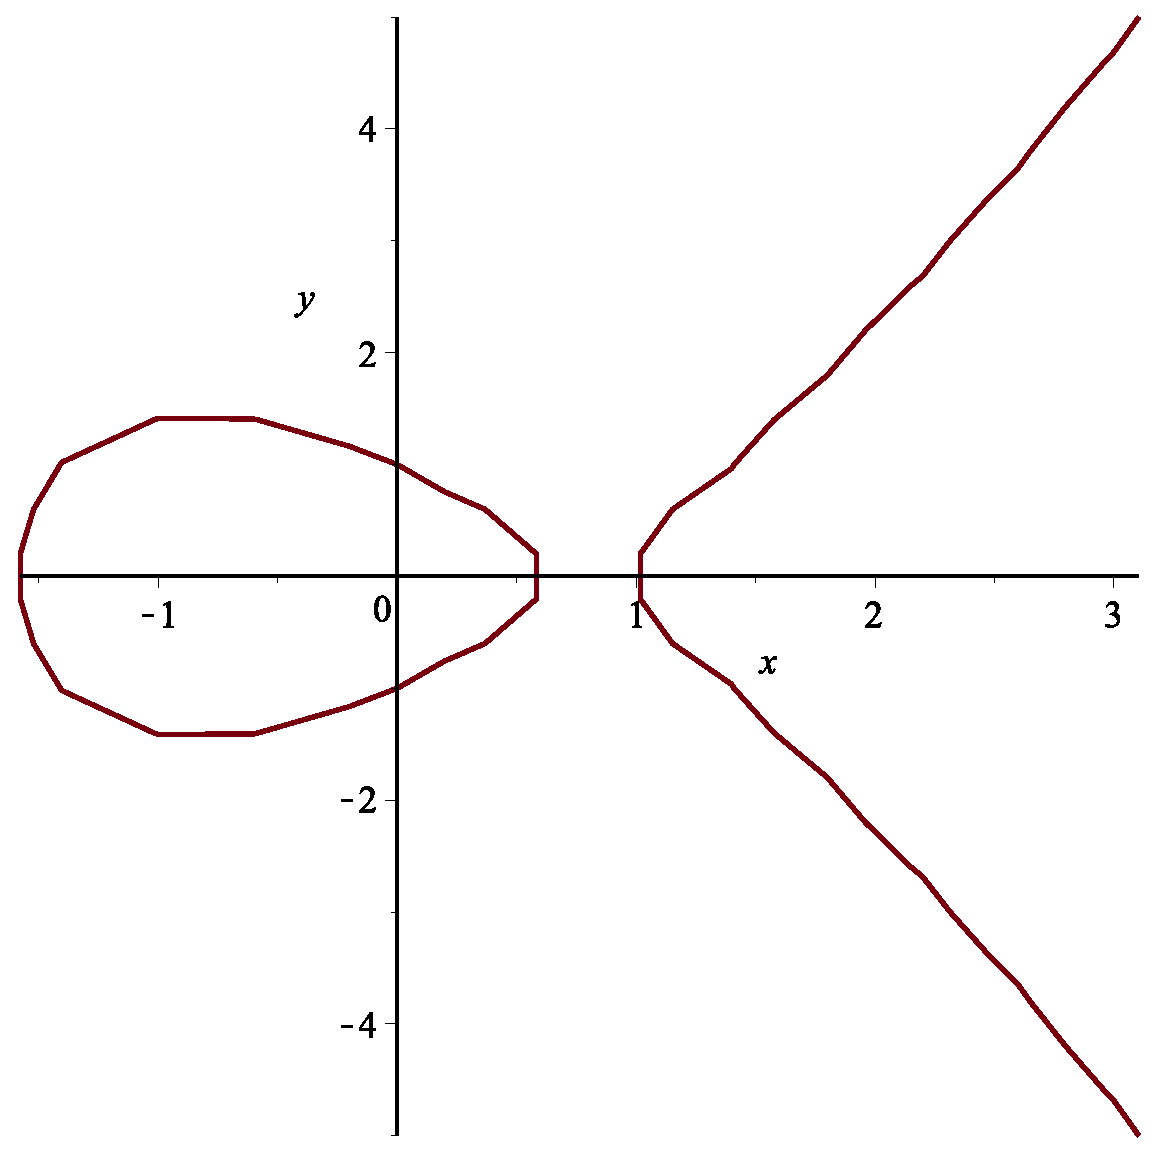
\includegraphics[scale=0.25]{tutorials/figures/Implicit_Functions_and_Graphsplot2d1-eps-converted-to.pdf}
\caption{Some versions of Maple may not produce a smooth plot of a curve, as shown here. In this case, you may need to increase the minimum number of points plotted by \texttt{implicitplot}. For example,\\
\texttt{> implicitplot(E, x=-5..5, y=-5..5, numpoints=30000);} \\
or \\
\texttt{> implicitplot(E, x=-5..5, y=-5..5, grid=[200,200]);} \\
Be careful not to choose too large of a value, otherwise the output may take a very long time to produce.}
\label{fig:plotresolution}
\end{marginfigure}

\index{implicit functions!implicitplot!filledregions}
\begin{maplegroup}
\begin{mapleinput}
\mapleinline{active}{1d}{implicitplot(L, x=-1.2..1.2, y=-1.2..1.8, coloring = ["red","blue"], filledregions=true);
}{}
\index{implicit functions!implicitplot!colour}
\end{mapleinput}
\mapleresult
\mapleplot{tutorials/figures/Implicit_Functions_and_Graphsplot2d3-eps-converted-to.pdf}
\end{maplegroup}

\section{Implicit Differentiation}
\label{sec:implicit_differentiation}

We need to use the \texttt{implicitdiff()} command to find the derivative of an implicit function. It is easiest to first assign a name to the equation.

\begin{maplegroup}
\begin{mapleinput}
\mapleinline{active}{1d}{E := y = x\symbol{94}2 + x;
}{}
\end{mapleinput}
\mapleresult
\begin{maplelatex}
\mapleinline{inert}{2d}{E := y = x^2+x}{\[\displaystyle E\, := \,y={x}^{2}+x\]}
\end{maplelatex}
\end{maplegroup}

\index{assignment operator!implicit function}
\index{packages!with}
\index{packages!plots}
\index{implicit functions!implicitplot!changing axes}
\index{implicit functions!implicitplot!plot resolution}
\index{implicit functions!implicitdiff}

\begin{maplegroup}
\begin{mapleinput}
\mapleinline{active}{1d}{with(plots):
}{}
\end{mapleinput}
\end{maplegroup}

\begin{maplegroup}
\begin{mapleinput}
\mapleinline{active}{1d}{implicitplot(E, x=-5..5, y=-5..5);
}{}
\end{mapleinput}
\mapleresult
\mapleplot{tutorials/figures/Implicit_Functions_and_Differentiationplot2d1-eps-converted-to.pdf}
\end{maplegroup}

\begin{maplegroup}
\begin{mapleinput}
\mapleinline{active}{1d}{dydx := implicitdiff(E, y, x);
}{}
\end{mapleinput}
\mapleresult
\begin{maplelatex}
\mapleinline{inert}{2d}{dydx := 2*x+1}{\[\displaystyle {\it dydx}\, := \,2\,x+1\]}
\end{maplelatex}
\end{maplegroup}

The order in which you list the variables matters; the first variable is treated as the dependent variable and the second variable is treated as the independent variable.
\marginnote{To find $dy/dx$, you must use \texttt{implicitdiff(E,y,x)} and to find $dx/dy$, you  must use \texttt{implicitdiff(E,x,y)}.}

\begin{maplegroup}
\begin{mapleinput}
\mapleinline{active}{1d}{dxdy := implicitdiff(E, x, y);
}{}
\end{mapleinput}
\mapleresult
\begin{maplelatex}
\mapleinline{inert}{2d}{dxdy := 1/(2*x+1)}{\[\displaystyle {\it dxdy}\, := \, \frac{1}{2\,x+1}\]}
\end{maplelatex}
\end{maplegroup}

When trying to find the slope of a tangent line at a point on an implicit curve, it helps to plot the curve first.

\index{mathematical functions!nth root@$n$\textsuperscript{th} root}

\begin{maplegroup}
\begin{mapleinput}
\mapleinline{active}{1d}{L := x\symbol{94}2 + (y - root[3](x\symbol{94}2))\symbol{94}2 = 1;
}{}
\end{mapleinput}
\mapleresult
\begin{maplelatex}
\mapleinline{inert}{2d}{L := x^2+(y-(x^2)^(1/3))^2 = 1}{\[\displaystyle L\, := \,{x}^{2}+ \left( y-\sqrt [3]{{x}^{2}} \right) ^{2}=1\]}
\end{maplelatex}
\end{maplegroup}

\begin{maplegroup}
\begin{mapleinput}
\mapleinline{active}{1d}{implicitplot(L, x=-1.2..1.2, y=-1.2..1.8);
}{}
\end{mapleinput}
\mapleresult
\mapleplot{tutorials/figures/Implicit_Functions_and_Differentiationplot2d2-eps-converted-to.pdf}
\end{maplegroup}

\noindent
To find the points on the curve at a specific $x$ value, you must first substitute the value and then solve for the $y$-coordinates.

\index{subs}
\index{solving equations!fsolve}

\begin{maplegroup}
\begin{mapleinput}
\mapleinline{active}{1d}{subs(x=0.5, L); yCoords := fsolve(%, y);
}{}
\end{mapleinput}
\mapleresult
\begin{maplelatex}
\mapleinline{inert}{2d}{.25+(y-.6299605249)^2 = 1}{\[\displaystyle  0.25+ \left( y- 0.6299605249 \right) ^{2}=1\]}
\end{maplelatex}
\marginnote{Notice that a list of two $y$-coordinates is assigned to a single name here. You could assign the individual values to unique names.}
\begin{maplelatex}
\mapleinline{inert}{2d}{yCoords := 1.495985929, -.2360648789}{\[\displaystyle {\it yCoords}\, := \, 1.495985929,\,- 0.2360648789\]}
\end{maplelatex}
\end{maplegroup}

\noindent
Then you can find the slopes of the tangent lines by computing the derivative with \texttt{implicitdiff()} and substituting the $x$ and $y$ values for each point.

\begin{maplegroup}
\begin{mapleinput}
\mapleinline{active}{1d}{dydx := implicitdiff(L, y, x);
}{}
\end{mapleinput}
\mapleresult
\begin{maplelatex}
\mapleinline{inert}{2d}{dydx := x*(-3*(x^2)^(2/3)-2*(x^2)^(1/3)+2*y)/(3(x^2)^(2/3)*y-x^2)}{\[\displaystyle {\it dydx}\, := \,{\frac {x \left( -3\, \left( {x}^{2} \right) ^{2/3}-2\,\sqrt [3]{{x}^{2}}+2\,y \right) }{ 3\left(y\left( {x}^{2} \right) ^{2/3}-{x}^{2}\right)}}\]}
\end{maplelatex}
\end{maplegroup}

\begin{maplegroup}
\begin{mapleinput}
\mapleinline{active}{1d}{subs(x=0.5, y=yCoords[1], dydx);
}{}
\end{mapleinput}
\mapleresult
\begin{maplelatex}
\mapleinline{inert}{2d}{.2625970976}{\[\displaystyle  0.2625970976\]}
\end{maplelatex}
\end{maplegroup}

\marginnote{\texttt{yCoords} is the name that both values are assigned to. To refer to an individual value, we use the index of the desired value in square brackets after the name \texttt{yCoords}.}

\begin{maplegroup}
\begin{mapleinput}
\mapleinline{active}{1d}{subs(x=0.5, y=yCoords[2], dydx);
}{}
\end{mapleinput}
\mapleresult
\begin{maplelatex}
\mapleinline{inert}{2d}{1.417297636}{\[\displaystyle  1.417297636\]}
\end{maplelatex}
\end{maplegroup}

\section{Applications of Implicit Differentiation}
\label{sec:applications_of_implicit_differentiation}

In these examples, we will make use of the \texttt{implicitdiff()} and \texttt{implicitplot()} commands.

\subsection{Finding the Equation of a Tangent Line}
\label{subsec:implicittanline}

\index{lines!tangent line!implicit function}

In this example, we will find the equations of the tangent lines to the circle of radius $4$, centred at the point $(1,1)$, where $x=3$. 
\marginnote{The equation of a circle that is centred at the point $(a,b)$ and has radius $r$ is
\[ (x-a)^2+(y-b)^2=r^2. \]}

\begin{maplegroup}
\begin{mapleinput}
\mapleinline{active}{1d}{circle := (x-1)\symbol{94}2 + (y-1)\symbol{94}2 = 16;
}{}
\end{mapleinput}
\mapleresult
\begin{maplelatex}
\mapleinline{inert}{2d}{circle := (x-1)^2+(y-1)^2 = 16}{\[\displaystyle {\it circle}\, := \,{(x-1)}^{2}+{(y-1)}^{2}=16\]}
\end{maplelatex}
\end{maplegroup}

We need to find the $y$-coordinates by substituting $x=3$ and solving for $y$.

\begin{maplegroup}
\begin{mapleinput}
\mapleinline{active}{1d}{subs(x=3, circle); yCoords:=solve(%, y);
}{}
\end{mapleinput}
\mapleresult
\begin{maplelatex}
\mapleinline{inert}{2d}{4+(y-1)^2 = 16}{\[\displaystyle 4+(y-1)^2 = 16\]}
\end{maplelatex}
\mapleresult
\begin{maplelatex}
\mapleinline{inert}{2d}{yCoords := 1+2\sqrt{3}, 1-2\sqrt(3)}{\[\displaystyle {\it yCoords}\, := \, 1+2\sqrt{3},\,1-2\sqrt{3}\]}
\end{maplelatex}
\end{maplegroup}

The derivative $\tfrac{dy}{dx}$ can be found using \texttt{implicitdiff()}. Then, by substituting the two points, we can find the slopes of both tangent lines.

\index{implicit functions!implicitdiff}
\index{subs}

\begin{maplegroup}
\begin{mapleinput}
\mapleinline{active}{1d}{dydx := implicitdiff(circle, y, x);
}{}
\end{mapleinput}
\mapleresult
\begin{maplelatex}
\mapleinline{inert}{2d}{dydx := -(x-1)/(y-1)}{\[\displaystyle {\it dydx}\, := \,-{\frac {x-1}{y-1}}\]}
\end{maplelatex}
\end{maplegroup}

\marginnote{Make sure that you choose different names when assigning values. We will need both slopes later.}

\begin{maplegroup}
\begin{mapleinput}
\mapleinline{active}{1d}{m1 := subs(x=3, y=yCoords[1], dydx);
}{}
\end{mapleinput}
\mapleresult
\begin{maplelatex}
\mapleinline{inert}{2d}{m1 := -\frac{1}{3}\sqrt{3}}{\[\displaystyle {\it m1}\, := \,-\frac{1}{3}\sqrt{3}\]}
\end{maplelatex}
\end{maplegroup}

\begin{maplegroup}
\begin{mapleinput}
\mapleinline{active}{1d}{m2 := subs(x=3, y=yCoords[2], dydx);
}{}
\end{mapleinput}
\mapleresult
\begin{maplelatex}
\mapleinline{inert}{2d}{m2 :=\frac{1}{3}\sqrt{3}}{\[\displaystyle {\it m2}\, := \,\frac{1}{3}\sqrt{3}\]}
\end{maplelatex}
\end{maplegroup}
\clearpage
Thinking ahead, in order to plot both lines using \texttt{implicitplot()}, they will need to be defined as \textit{equations}.

\index{subs}

\begin{maplegroup}
\begin{mapleinput}
\mapleinline{active}{1d}{line1 := y = m1*(x-3) + yCoords[1];expand(\%);
}{}
\end{mapleinput}
\mapleresult
\begin{maplelatex}
\mapleinline{inert}{2d}{line1 := y = -\frac{1}{3}\sqrt{3}(x-3)+1+2\sqrt{3}}{\[\displaystyle {\it line1}\, := \,y=-\frac{1}{3}\sqrt{3}(x-3)+1+2\sqrt{3}\]}
\end{maplelatex}
\begin{maplelatex}
\mapleinline{inert}{2d}{y = -\frac{1}{3}\sqrt{3}x+3\sqrt{3}+1}{\[\displaystyle  y=-\frac{1}{3}\sqrt{3}x+3\sqrt{3}+1\]}
\end{maplelatex}
\end{maplegroup}

\marginnote{Both \texttt{line1} and \texttt{line2} are defined with the inclusion of $y=$, making them equations that \texttt{implicitplot()} can plot.}

\begin{maplegroup}
\begin{mapleinput}
\mapleinline{active}{1d}{line2 := y = m2*(x-3) + yCoords[2];expand(\%);
}{}
\end{mapleinput}
\mapleresult
\begin{maplelatex}
\mapleinline{inert}{2d}{line2 := y = \frac{1}{3}\sqrt{3}(x-3)+1-2\sqrt{3}}{\[\displaystyle {\it line2}\, := \,y=\frac{1}{3}\sqrt{3}(x-3)+1-2\sqrt{3}\]}
\end{maplelatex}
\begin{maplelatex}
\mapleinline{inert}{2d}{y = \frac{1}{3}\sqrt{3}x-3\sqrt{3}+1}{\[\displaystyle  y=\frac{1}{3}\sqrt{3}x-3\sqrt{3}+1\]}
\end{maplelatex}
\end{maplegroup}

We can now plot the circle and the two lines together.

\index{packages!plots}
\index{implicit functions!implicitplot!scaling}
\index{implicit functions!implicitplot!multiple curves}
\index{implicit functions!implicitplot!changing axes}
\index{implicit functions!implicitplot!plot resolution}
\index{implicit functions!implicitplot!colour}

\begin{maplegroup}
\begin{mapleinput}
\mapleinline{active}{1d}{with(plots):
}{}
\end{mapleinput}
\end{maplegroup}

\begin{maplegroup}
\begin{mapleinput}
\mapleinline{active}{1d}{implicitplot([circle, line1, line2], x=-8..8, y=-8..8, colour=[red,blue,green], scaling=constrained);
}{}
\end{mapleinput}
\mapleresult
\mapleplot{tutorials/figures/ImplicitTangentCircle.eps}
\end{maplegroup}

\marginnote[-4cm]{Using the \texttt{scaling=constrained} parameter will produce a proper circle in your worksheet. The graph can also be scaled without using the \texttt{scaling=constrained} parameter; simply click on the graph and then click on the 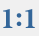
\includegraphics[scale=0.5]{tutorials/figures/1-1.png} button in the plot toolbar at the top of the page.}

\subsection{Orthogonal Curves}
\label{subsec:orthocurves}

In this example, we will show that the curves $x^2 - y^2 = 8$ and $-xy =~3$ are always perpendicular (orthogonal) at their intersection points.

\begin{maplegroup}
\begin{mapleinput}
\mapleinline{active}{1d}{curve1 := x\symbol{94}2 - y\symbol{94}2 = 8;
}{}
\end{mapleinput}
\mapleresult
\begin{maplelatex}
\mapleinline{inert}{2d}{curve1 := x^2-y^2 = 8}{\[\displaystyle {\it curve1}\, := \,{x}^{2}-{y}^{2}=8\]}
\end{maplelatex}
\end{maplegroup}


\begin{maplegroup}
\begin{mapleinput}
\mapleinline{active}{1d}{curve2 := -x*y = 3;
}{}
\end{mapleinput}
\mapleresult
\begin{maplelatex}
\mapleinline{inert}{2d}{curve2 := -x*y = 23}{\[\displaystyle {\it curve2}\, := \,-xy=3\]}
\end{maplelatex}
\end{maplegroup}

\begin{maplegroup}
\begin{mapleinput}
\mapleinline{active}{1d}{with(plots):
}{}
\end{mapleinput}
\end{maplegroup}

\marginnote[-1.5cm]{We must include multiplication between $x$ and $y$ here, otherwise Maple will think we want to use a variable called $xy$.}

\begin{maplegroup}
\begin{mapleinput}
\mapleinline{active}{1d}{implicitplot([curve1, curve2], x=-5..5, y=-5..5, colour=[red, blue], scaling=constrained);
}{}
\end{mapleinput}
\mapleresult
\mapleplot{tutorials/figures/OrthogonalCurves2.eps}
\end{maplegroup}

\marginnote[-1cm]{Using the \texttt{scaling=constrained} parameter will preserve right angles in your worksheet.}

From the graphs of these two curves, it appears that their intersections are perpendicular. This can be proven by showing that the derivative of one curve is equal to the negative reciprocal of the other, or that they multiply to equal $-1$.

The intersection points can be found by solving a system of equations.

\index{solving equations!intersection points}
\index{implicit functions!implicitdiff}
\index{subs}

\marginnote[0.5cm]{Using the option \texttt{explicit=true} here will avoid the use of \textit{RootOf} in the output. Optionally, using \texttt{fsolve()} may be preferable. Points involving $I$ are imaginary points and should not be considered.}

\begin{maplegroup}
\begin{mapleinput}
\mapleinline{active}{1d}{solve(\{curve1, curve2\}, \{x, y\}, explicit = true);
}{}
\end{mapleinput}
\mapleresult
\begin{maplelatex}
\mapleinline{inert}{2d}{{x = -3, y = 1}, {x = 3, y = -1}, {x = I, y = 3*I}, {x = -I, y = -3*I}}{\[\displaystyle  \left\{ x=-3,y=1 \right\} ,\, \left\{ x=3,y=-1 \right\} ,\, \left\{ x=I,y=3\,I \right\} ,\, \left\{ x= -I,y=-3\,I \right\} \]}
\end{maplelatex}
\end{maplegroup}

The derivatives of both curves can be found implicitly using the \texttt{implicitdiff()} command.

\begin{maplegroup}
\begin{mapleinput}
\mapleinline{active}{1d}{dydx1 := implicitdiff(curve1, y, x);
}{}
\end{mapleinput}
\mapleresult
\begin{maplelatex}
\mapleinline{inert}{2d}{dydx1 := x/y}{\[\displaystyle {\it dydx1}\, := \,{\frac {x}{y}}\]}
\end{maplelatex}
\end{maplegroup}

\begin{maplegroup}
\begin{mapleinput}
\mapleinline{active}{1d}{dydx2 := implicitdiff(curve2, y, x);
}{}
\end{mapleinput}
\mapleresult
\begin{maplelatex}
\mapleinline{inert}{2d}{dydx2 := -y/x}{\[\displaystyle {\it dydx2}\, := \,-{\frac {y}{x}}\]}
\end{maplelatex}
\end{maplegroup}

To show that the slopes are negative reciprocals, a point can be substituted into the two derivatives.

\begin{maplegroup}
\begin{mapleinput}
\mapleinline{active}{1d}{subs(x=-3, y=1, dydx1);
}{}
\end{mapleinput}
\mapleresult
\begin{maplelatex}
\mapleinline{inert}{2d}{-3}{\[\displaystyle -3\]}
\end{maplelatex}
\begin{mapleinput}
\mapleinline{active}{1d}{subs(x=-3, y=1, dydx2);
}{}
\end{mapleinput}
\mapleresult
\begin{maplelatex}
\mapleinline{inert}{2d}{\frac{1}{3}}{\[\displaystyle \frac{1}{3}\]}
\end{maplelatex}
\end{maplegroup}

Alternatively, it can be shown that the derivatives are negative reciprocals of each other in general.

\marginnote{Recall that two slopes $m_1$ and $m_2$ are perpendicular if $m_1 m_2 = -1$.}

\begin{maplegroup}
\begin{mapleinput}
\mapleinline{active}{1d}{dydx1*dydx2;
}{}
\end{mapleinput}
\mapleresult
\begin{maplelatex}
\mapleinline{inert}{2d}{-1}{\[\displaystyle -1\]}
\end{maplelatex}
\end{maplegroup}
\chapter{Riemann Sums and Approximations of Area}
\label{chp:riemann_sums_and_area_approximation}	

In this tutorial, we use numerical approximation to calculate definite integrals (namely, the right-sum, left-sum, midpoint, Simpson's, and trapezoidal methods). We then calculate these definite integrals using the Fundamental Theorem of Calculus. We will also learn how to find indefinite integrals as functions.

\section{Approximating the Area Under a Function Using ApproximateInt}
\label{sec:approximating_area_using_approximateint}

To use the \texttt{ApproximateInt()} command, we must load the \\
\noindent\texttt{Student[Calculus1]} package.

The function and interval must be specified. Other optional parameters may be included to change how the result is displayed and how the approximation is computed.

\index{integral approximation!ApproximateInt}
\index{integral approximation!ApproximateInt!method}
\index{integral approximation!ApproximateInt!output options}
\index{integral approximation!ApproximateInt!partition}

\begin{table}
\label{tbl:approximateint_options}
\centering
\begin{tabular}{lp{2.5in}}
\hline
Parameter & Description\\
\hline
\texttt{method = }\textit{method}	& Select the method for approximation (\texttt{left}, \texttt{right}, \texttt{lower}, 
									\texttt{upper}, \texttt{midpoint}, \texttt{trapezoid}, \texttt{simpson}).\\
\texttt{output = }\textit{output}	& Change how the output is displayed (\texttt{plot}, \texttt{value}, \texttt{sum}).\\
\texttt{partition = $n$}			& Change the number of subintervals to use for approximation.\\
\hline
\end{tabular}
\caption{A list of optional parameters for the \texttt{ApproximateInt()} command.}
\end{table}

Most of these methods of approximation are discussed in class: left-point, right-point, midpoint rule, trapezoid rule, and Simpson's rule. When using \texttt{method=upper}, the height of each rectangle corresponds to the maximum value of the function in each subinterval. Similarly, when using \texttt{method=lower}, the height of each rectangle corresponds to the minimum value of the function in each subinterval. 

\subsection{Approximating the Area under $10 {\rm e}^{-x}$}

We can use different methods for the rectangles, such as left-point and right-point. Let's define a function, $f(x)$ and calculate some approximations.
\marginnote[-1cm]{These are two common methods that we learn when first calculating Riemann sums.}

\index{mathematical functions!exponential}

\begin{maplegroup}
\begin{mapleinput}
\mapleinline{active}{1d}{f(x) := 10*exp(-x);
}{}
\end{mapleinput}
\mapleresult
\begin{maplelatex}
\mapleinline{inert}{2d}{f := proc (x) options operator, arrow; 10*exp(-x) end proc}{\[\displaystyle f\, := \,x\mapsto 10\,{{\rm e}^{-x}}\]}
\end{maplelatex}
\end{maplegroup}

\begin{maplegroup}
\begin{mapleinput}
\mapleinline{active}{1d}{ApproximateInt(f(x), x = 0..4, method=left, output=value, partition=8); evalf(%);
}{}
\end{mapleinput}
\mapleresult
\begin{maplelatex}
\mapleinline{inert}{2d}{5+5*exp(-1/2)+5*exp(-1)+5*exp(-3/2)+5*exp(-2)+5*exp(-5/2)+5*exp(-3)+5*exp(-7/2)}{\[\displaystyle 5+5\,{{\rm e}^{-1/2}}+5\,{{\rm e}^{-1}}+5\,{{\rm e}^{-3/2}}+5\,{{\rm e}^{-2}}+5\,{{\rm e}^{-5/2}}+5\,{{\rm e}^{-3}}
+5\,{{\rm e}^{-7/2}}\]}
\end{maplelatex}
\mapleresult
\begin{maplelatex}
\mapleinline{inert}{2d}{12.47472497}{\[\displaystyle  12.47472497\]}
\end{maplelatex}
\end{maplegroup}

\begin{maplegroup}
\begin{mapleinput}
\mapleinline{active}{1d}{ApproximateInt(f(x), x = 0..4, method=right, output=value, partition=8); evalf(%);
}{}
\end{mapleinput}
\mapleresult
\begin{maplelatex}
\mapleinline{inert}{2d}{5*exp(-1/2)+5*exp(-1)+5*exp(-3/2)+5*exp(-2)+5*exp(-5/2)+5*exp(-3)+5*exp(-7/2)+5*exp(-4)}{\[\displaystyle 5\,{{\rm e}^{-1/2}}+5\,{{\rm e}^{-1}}+5\,{{\rm e}^{-3/2}}+5\,{{\rm e}^{-2}}+5\,{{\rm e}^{-5/2}}+5\,{{\rm e}^{-3}}+5\,{{\rm e}^{-7/2}}+5\,{{\rm e}^{-4}}\]}
\end{maplelatex}
\mapleresult
\begin{maplelatex}
\mapleinline{inert}{2d}{7.566303166}{\[\displaystyle  7.566303166\]}
\end{maplelatex}
\end{maplegroup}

\index{integral approximation!ApproximateInt}
\index{integral approximation!ApproximateInt!method}
\index{integral approximation!ApproximateInt!output options}
\index{integral approximation!ApproximateInt!partition}
\index{integral approximation!Riemann sum}
\index{evalf}
\index{ditto operator}
\index{limit!at infinity}

If we wish to get the actual area under the curve, we can give the Riemann sum for $n$ rectangles and take the limit as $n\rightarrow\infty$.

\marginnote[1cm]{In some cases, Maple may not output this limit as a numerical value. Using the \texttt{value(\%)} command after the limit may help to convert the limit to a numerical result.}
\begin{maplegroup}
\begin{mapleinput}
\mapleinline{active}{1d}{ApproximateInt(f(x), x = 0..4, method=left, output=sum, partition=n); limit(%, n=infinity); evalf(%);}{}
\end{mapleinput}
\mapleresult
\begin{maplelatex}
\mapleinline{inert}{2d}{4*(Sum(10*exp(-4*i/n), i = 0 .. n-1))/n}{\[\displaystyle 4\,{\frac {1}{n}\sum _{i=0}^{n-1}10\,{{\rm e}^{-4\,{\frac {i}{n}}}}}\]}
\end{maplelatex}
\mapleresult
\begin{maplelatex}
\mapleinline{inert}{2d}{10-10*exp(-4)}{\[\displaystyle 10-10\,{{\rm e}^{-4}}\]}
\end{maplelatex}
\mapleresult
\begin{maplelatex}
\mapleinline{inert}{2d}{9.816843611}{\[\displaystyle  9.816843611\]}
\end{maplelatex}
\end{maplegroup}

\subsection{Approximating the Area under $x \sin(x)$}

We can define a function and approximate the area under the curve over a specified interval. In this example, we will use the \texttt{upper}, \texttt{lower}, and \texttt{midpoint} methods for approximating rectangles.

\index{packages!Student[Calculus1]}

\begin{maplegroup}
\begin{mapleinput}
\mapleinline{active}{1d}{with(Student[Calculus1]):
}{}
\end{mapleinput}
\end{maplegroup}

\index{mathematical functions!sine}

\begin{maplegroup}
\begin{mapleinput}
\mapleinline{active}{1d}{f(x) := x*sin(x);
}{}
\end{mapleinput}
\mapleresult
\begin{maplelatex}
\mapleinline{inert}{2d}{f := proc (x) options operator, arrow; x*sin(x) end proc}{\[\displaystyle f\, := \,x\mapsto x\sin \left( x \right) \]}
\end{maplelatex}
\end{maplegroup}

\begin{maplegroup}
\begin{mapleinput}
\mapleinline{active}{1d}{ApproximateInt(f(x), x=-3..3, method=upper, output=plot, partition=10);
}{}
\end{mapleinput}
\marginnote[-2cm]{The \texttt{method=upper} parameter always uses the \textbf{highest} rectangle in an interval. This will force an overestimate of the actual area underneath the curve.}
\mapleresult
\mapleplot{tutorials/figures/Riemann_Sumsplot2d1-eps-converted-to.pdf}
\end{maplegroup}
\marginnote[-0.5cm]{The \texttt{method=lower} parameter always uses the \textbf{lowest} rectangle in an interval. This will force an underestimate of the actual area underneath the curve.}

\begin{maplegroup}
\begin{mapleinput}
\mapleinline{active}{1d}{ApproximateInt(f(x), x=-3..3, method=upper, output=value, partition=10);}{}
\end{mapleinput}
\mapleresult
\begin{maplelatex}
\mapleinline{inert}{2d}{7.981170598}{\[\displaystyle  7.981170598\]}
\end{maplelatex}
\end{maplegroup}

\begin{maplegroup}
\begin{mapleinput}
\mapleinline{active}{1d}{ApproximateInt(f(x), x=-3..3, method=lower, output=value, partition=10);}{}
\end{mapleinput}
\mapleresult
\begin{maplelatex}
\mapleinline{inert}{2d}{4.202044853}{\[\displaystyle  4.202044853\]}
\end{maplelatex}
\end{maplegroup}

\index{integral approximation!ApproximateInt}
\index{integral approximation!ApproximateInt!method}
\index{integral approximation!ApproximateInt!output options}
\index{integral approximation!ApproximateInt!partition}
\begin{maplegroup}
\begin{mapleinput}
\mapleinline{active}{1d}{ApproximateInt(f(x), x=-3..3, method=midpoint, output=plot, partition=20);}{}
\end{mapleinput}
\mapleresult
\mapleplot{tutorials/figures/Riemann_Sumsplot2d2-eps-converted-to.pdf}
\end{maplegroup}

\section{Approximating the Value of a Definite Integral}
\label{sec:approximating_a_definite_integral}

We can also set up an integral to use numerical approximation on.

\marginnote{Use of the \texttt{Int()} command will be fully explained in Tutorial \ref{chp:definite_and_indefinite_Integrals} on page \pageref{chp:definite_and_indefinite_Integrals}.}
\begin{maplegroup}
\begin{mapleinput}
\mapleinline{active}{1d}{int1 := Int(x\symbol{94}2, x=0..2);
}{}
\end{mapleinput}
\mapleresult
\begin{maplelatex}
\mapleinline{inert}{2d}{int1 := Int(x^2, x = 0 .. 2)}{\[\displaystyle {\it int1}\, := \,\int _{0}^{2}\!{x}^{2}{dx}\]}
\end{maplelatex}
\end{maplegroup}

\index{integral!Int}

We can evaluate this integral with $4$ subintervals using three different methods.

\begin{maplegroup}
\begin{mapleinput}
\mapleinline{active}{1d}{ApproximateInt(int1, method=midpoint, output=value, partition=4);
}{}
\end{mapleinput}
\mapleresult
\begin{maplelatex}
\mapleinline{inert}{2d}{21/8}{\[\displaystyle {\frac {21}{8}}\]}
\end{maplelatex}
\end{maplegroup}

\begin{maplegroup}
\begin{mapleinput}
\mapleinline{active}{1d}{ApproximateInt(int1, method=trapezoid, output=value, partition=4);
}{}
\end{mapleinput}
\index{integral approximation!ApproximateInt!method}
\marginnote[-0.5cm]{The \texttt{method=trapezoid} parameter uses trapezoid shapes instead of rectangles to approximate the area. This usually gives a more accurate estimate of the area.}
\mapleresult
\begin{maplelatex}
\mapleinline{inert}{2d}{11/4}{\[\displaystyle \frac{11}{4}\]}
\end{maplelatex}
\end{maplegroup}

\begin{maplegroup}
	\begin{mapleinput}
		\mapleinline{active}{1d}{ApproximateInt(int1, method=simpson, output=value, partition=4);
		}{}
	\end{mapleinput}
	\mapleresult
	\begin{maplelatex}
		\mapleinline{inert}{2d}{8/3}{\[\displaystyle \frac{8}{3}\]}
	\end{maplelatex}
\end{maplegroup}

\index{integral approximation!ApproximateInt!method}
\marginnote[-1.5cm]{When using Simpson's rule, an additional sample point is used per subinterval. So, if $n$ subintervals are used, then the number of sample points is $2n$.}
Simpson's rule uses twice as many sample points as the other two methods used here. If we wish to have $4$ points used for Simpson's rule, we use \texttt{partition=2}.

To visualize the approximation using any of the above methods, we use the option \texttt{output=plot}.

\begin{maplegroup}
\begin{mapleinput}
\mapleinline{active}{1d}{ApproximateInt(int1, method=trapezoid, output=plot, partition=2);
}{}
\end{mapleinput}
\marginnote[-0.5cm]{Notice that trapezoidal shapes are used instead of rectangles.}
\mapleresult
\mapleplot{tutorials/figures/numerical_integration_using_ApproximateIntplot2d1-eps-converted-to.pdf}
\end{maplegroup}

\index{integral approximation!ApproximateInt!method}
\index{integral approximation!ApproximateInt}
\index{integral approximation!ApproximateInt!method}
\index{integral approximation!ApproximateInt!output options}
\index{integral approximation!ApproximateInt!partition}

\noindent
Maple can also give the Riemann sum for any of the above approximations.

\begin{maplegroup}
\begin{mapleinput}
\mapleinline{active}{1d}{ApproximateInt(int1, method=trapezoid, output=sum, partition=4);
}{}
\end{mapleinput}
\marginnote[0.5cm]{The \texttt{output=sum} shows you what the expanded summation looks like \textbf{before} it is evaluated.}
\mapleresult
\begin{maplelatex}
\mapleinline{inert}{2d}{(1/4)*(Sum((1/4)*i^2+((1/2)*i+1/2)^2, i = 0 .. 3))}{\[\displaystyle \frac{1}{4}\,\sum _{i=0}^{3}\frac{1}{4}\,{i}^{2}+ \left( \frac{1}{2}\,i+\frac{1}{2} \right) ^{2}\]}
\end{maplelatex}
\end{maplegroup}
\chapter{Definite and Indefinite Integrals}
\label{chp:definite_and_indefinite_Integrals}	

\section{Definite Integrals}
\label{sec:definite_integrals}

We now turn our attention to using the Fundamental Theorem of Calculus to calculate definite integrals to (in most cases) obtain the area underneath a curve.\\

The \texttt{int()} command allows us to compute integrals (both definite and indefinite) directly. The \texttt{Int()} command allows us to symbolically view the integral, or assign it to a variable to use later for other computations or calculations. Capitalization is important in Maple.

\subsection{The Definite Integral $\displaystyle\int_{-3}^{3}\frac{1}{x^2+1}\, dx$}

\begin{maplegroup}
\begin{mapleinput}
\mapleinline{active}{1d}{f(x) := 1/(1+x\symbol{94}2);
}{}
\end{mapleinput}
\mapleresult
\begin{maplelatex}
\mapleinline{inert}{2d}{f := proc (x) options operator, arrow; 1/(1+x^2) end proc}{\[\displaystyle f\, := \,x\mapsto  \frac{1}{ {x}^{2}+1 }\]}
\end{maplelatex}
\end{maplegroup}
\begin{maplegroup}
\begin{mapleinput}
\mapleinline{active}{1d}{plot(f(x), x=-3..3);
}{}
\end{mapleinput}
\mapleresult
\mapleplot{tutorials/figures/Definite_And_Indefinite_Integralsplot2d1-eps-converted-to.pdf}
\end{maplegroup}

\index{plot!axes intervals}
\index{integral!int!definite}
\index{integral!Int!definite}

We use the \texttt{Int()} command to display the integral, and the \texttt{int()} command to evaluate the integral.

\begin{maplegroup}
\begin{mapleinput}
\mapleinline{active}{1d}{Int(f(x), x=-3..3);
}{}
\end{mapleinput}
\marginnote{Note the capital ``I" in this command. This prevents Maple from automatically evaluating the integral.}
\mapleresult
\begin{maplelatex}
\mapleinline{inert}{2d}{Int(1/(x^2+1), x = -3 .. 3)}{\[\displaystyle \int _{-3}^{3}\! \frac{1}{ {x}^{2}+1 }\,{dx}\]}
\end{maplelatex}
\end{maplegroup}

\begin{maplegroup}
\begin{mapleinput}
\mapleinline{active}{1d}{int(f(x), x=-3..3); evalf(%);
}{}
\end{mapleinput}
\mapleresult
\begin{maplelatex}
\mapleinline{inert}{2d}{2*arctan(3)}{\[\displaystyle 2\,\arctan \left( 3 \right) \]}
\end{maplelatex}
\begin{maplelatex}
\mapleinline{inert}{2d}{2.498091544}{\[\displaystyle  2.498091544\]}
\end{maplelatex}
\end{maplegroup}

\subsection{The Definite Integral $\displaystyle\int_{1}^{10} \ln(x) \, dx$}	

\index{mathematical functions!logarithmic@natural logarithmic}

\begin{maplegroup}
\begin{mapleinput}
\mapleinline{active}{1d}{g(x) := ln(x);
}{}
\end{mapleinput}
\mapleresult
\begin{maplelatex}
\mapleinline{inert}{2d}{g := proc (x) options operator, arrow; ln(x) end proc}{\[\displaystyle g\, := \,x\mapsto \ln  \left( x \right) \]}
\end{maplelatex}
\end{maplegroup}
\begin{maplegroup}
\begin{mapleinput}
\mapleinline{active}{1d}{plot(g(x), x=1..10);
}{}
\end{mapleinput}
\mapleresult
\mapleplot{tutorials/figures/Definite_And_Indefinite_Integralsplot2d2-eps-converted-to.pdf}
\end{maplegroup}
\begin{maplegroup}
\begin{mapleinput}
\mapleinline{active}{1d}{int(g(x), x=1..10); evalf(%);
}{}
\end{mapleinput}
\mapleresult
\begin{maplelatex}
\mapleinline{inert}{2d}{-9+10*ln(2)+10*ln(5)}{\[\displaystyle -9+10\,\ln  \left( 2 \right) +10\,\ln  \left( 5 \right) \]}
\end{maplelatex}
\begin{maplelatex}
\mapleinline{inert}{2d}{14.02585093}{\[\displaystyle  14.02585093\]}
\end{maplelatex}
\end{maplegroup}

\index{plot!axes intervals}
\index{integral!int!definite}
\index{evalf}
\index{ditto operator}

\subsection{Improper Integrals}

\index{integral!int!improper}
\index{integral!Int!improper}

The \texttt{int()} and \texttt{Int()} commands can also be used to compute improper integrals.

\begin{maplegroup}
\begin{mapleinput}
\mapleinline{active}{1d}{h(x) := 1/x\symbol{94}2;
}{}
\end{mapleinput}
\mapleresult
\begin{maplelatex}
\mapleinline{inert}{2d}{h := proc (x) options operator, arrow; 1/x^2 end proc}{\[\displaystyle h\, := \,x\mapsto {x}^{-2}\]}
\end{maplelatex}
\end{maplegroup}
\begin{maplegroup}
\begin{mapleinput}
\mapleinline{active}{1d}{plot(h(x), x=0..infinity);
}{}
\end{mapleinput}
\mapleresult
\mapleplot{tutorials/figures/Definite_And_Indefinite_Integralsplot2d3-eps-converted-to.pdf}
\end{maplegroup}
\begin{maplegroup}
\begin{mapleinput}
\mapleinline{active}{1d}{Int(h(x), x=1..infinity);
}{}
\end{mapleinput}
\mapleresult
\begin{maplelatex}
\mapleinline{inert}{2d}{Int(1/x^2, x = 1 .. infinity)}{\[\displaystyle \int _{1}^{\infty }\!{x}^{-2}{dx}\]}
\end{maplelatex}
\end{maplegroup}
\begin{maplegroup}
\begin{mapleinput}
\mapleinline{active}{1d}{int(h(x), x=1..infinity);
}{}
\end{mapleinput}
\mapleresult
\begin{maplelatex}
\mapleinline{inert}{2d}{1}{\[\displaystyle 1\]}
\end{maplelatex}
\end{maplegroup}

\section{Indefinite Integrals and Antiderivatives}
\label{sec:indefinite_integrals_and_antiderivatives}

If we do not have limits of integration we still can use the \texttt{Int()} and \texttt{int()} commands to show and evaluate the integrals respectively.

\index{integral!int!indefinite}
\index{integral!Int!indefinite}
\index{mathematical functions!square root}

\marginnote{Recall that \texttt{Int()} displays the integral and \texttt{int()} evaluates the integral.}
\begin{maplegroup}
\begin{mapleinput}
\mapleinline{active}{1d}{Int(sin(x), x);
}{}
\end{mapleinput}
\mapleresult
\begin{maplelatex}
\mapleinline{inert}{2d}{Int(sin(x), x)}{\[\displaystyle \int \!\sin \left( x \right) {dx}\]}
\end{maplelatex}
\end{maplegroup}

\begin{maplegroup}
\begin{mapleinput}
\mapleinline{active}{1d}{int(sin(x), x);
}{}
\end{mapleinput}
\mapleresult
\begin{maplelatex}
\mapleinline{inert}{2d}{-cos(x)}{\[\displaystyle -\cos \left( x \right) \]}
\end{maplelatex}
\end{maplegroup}

\marginnote[-1cm]{Maple does not include the addition of the constant of integration $+C$ when evaluating indefinite integrals.}

\begin{maplegroup}
\begin{mapleinput}
\mapleinline{active}{1d}{p(x) := 1/sqrt(1 + x\symbol{94}2);
}{}
\end{mapleinput}
\mapleresult
\begin{maplelatex}
\mapleinline{inert}{2d}{p := proc (x) options operator, arrow; 1/sqrt(1+x^2) end proc}{\[\displaystyle p\, := \,x\mapsto {\frac {1}{\sqrt {{x}^{2}+1}}}\]}
\end{maplelatex}
\end{maplegroup}

\begin{maplegroup}
\begin{mapleinput}
\mapleinline{active}{1d}{Int(p(x), x);
}{}
\end{mapleinput}
\mapleresult
\begin{maplelatex}
\mapleinline{inert}{2d}{Int(1/sqrt(x^2+1), x)}{\[\displaystyle \int \! \left(  \sqrt{{x}^{2}+1} \right) ^{-1}{dx}\]}
\end{maplelatex}
\end{maplegroup}
\marginnote[-1cm]{The function arcsinh$()$ is called the inverse hyperbolic sine function. Functions like $\cosh()$ and $\sinh()$ are called hyperbolic functions. These functions are analogs of the ordinary trigonometric, or circular, functions; just as the points $(\cos(t), \sin(t))$ form a circle with a unit radius, the points $(\cosh(t), \sinh(t))$ form the right half of the equilateral hyperbola.}
\index{mathematical functions!inverse hyperbolic sine}
        \index{mathematical functions!hyperbolic functions!sinh}
         \index{mathematical functions!hyperbolic functions!cosh}
\begin{maplegroup}
\begin{mapleinput}
\mapleinline{active}{1d}{int(p(x), x);
}{}
\end{mapleinput}
\mapleresult
\begin{maplelatex}
\mapleinline{inert}{2d}{arcsinh(x)}{\[\displaystyle {\it arcsinh} \left( x \right) \]}
\end{maplelatex}
\end{maplegroup}

\section{The Integration Methods Tutor}
\label{sec:the_integration_methods_tutor}
\index{integral!integration methods tutor}

The Integration Methods tutor can be used to evaluate an integral step-by-step. You can either manually attempt different techniques on the integral, or let Maple decide which techniques to use. 

\begin{figure}[h]
\caption{Opening up the Integration Methods tutor using menus.}
\centering
\adjincludegraphics[width=\textwidth]{tutorials/figures/IntTutorLoad1-eps-converted-to.pdf}
\end{figure}

\begin{figure}[h]
\caption{Opening up the Integration Methods tutor using commands. The \texttt{Student[Calculus1]} package is required.}
\centering
\adjincludegraphics[width=\textwidth]{tutorials/figures/IntTutorLoad2-eps-converted-to.pdf}
\\
\end{figure}

\clearpage

\subsection{Evaluating $\displaystyle\int x^2e^x$ Using Integration by Parts}

\index{integral!integration methods tutor}

\begin{figure}[h]
\caption{If the Get Hint button is clicked, Maple will suggest an integration technique.}
\centering
\adjincludegraphics[width=0.8\textwidth,trim={0 {0.2\height} 0 0},clip]{tutorials/figures/IntTutorQ1-1-eps-converted-to.pdf}
\end{figure}

\marginnote[-4cm]{When typing out the function in the tutor, you will not have access to the palettes toolbar in Maple. You will need to type out commands such as \texttt{sqrt()} for square roots. You must also include the symbol * for multiplication.}

\begin{figure}[h]
\caption{Integration by parts  can be applied to integrals of the form $\int u~dv$, where $u=f(x)$ and $dv = g'(x) dx$.}
\centering
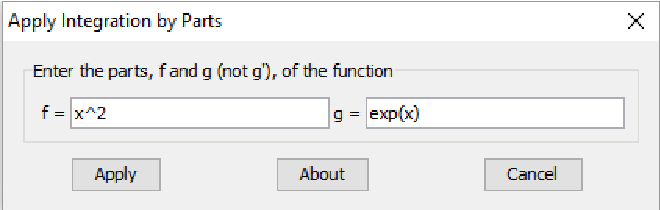
\includegraphics[width=0.6\textwidth]{tutorials/figures/IntTutorQ1-2-eps-converted-to.pdf}
\adjincludegraphics[width=0.8\textwidth,trim={0 {0.5\height} 0 0},clip]{tutorials/figures/IntTutorQ1-3-eps-converted-to.pdf}
\end{figure}

\begin{figure}[h]
\caption{Using the constant multiple rule, integration by parts a second time, and the exponential rule to evaluate the integral.}
\centering
\adjincludegraphics[width=0.8\textwidth,trim={0 {0.2\height} 0 0},clip]{tutorials/figures/IntTutorQ1-4-eps-converted-to.pdf}\\
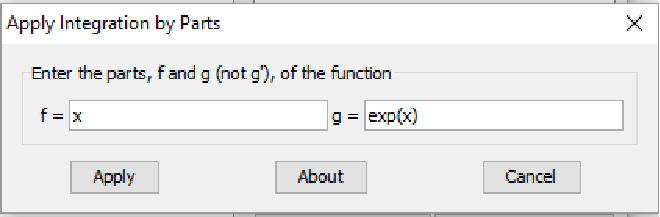
\includegraphics[width=0.6\textwidth]{tutorials/figures/IntTutorQ1-5-eps-converted-to.pdf}
\adjincludegraphics[width=0.8\textwidth,trim={0 {0.2\height} 0 0},clip]{tutorials/figures/IntTutorQ1-6-eps-converted-to.pdf}\\
\end{figure}

\clearpage

\subsection{Evaluating $\displaystyle\int_{-\pi/2}^{\pi/4} x\sin(x^2+1)$ Using Substitution}

\index{integral!integration methods tutor}

\begin{figure}[h]
\caption{If you use the All Steps button, then Maple will evaluate the integral, showing all steps.}
\centering
\adjincludegraphics[width=0.8\textwidth,trim={0 0 0 0},clip]{tutorials/figures/IntTutorQ2-eps-converted-to.pdf}\\
\end{figure}

\clearpage

\section{Volumes of Revolution}
\label{sec:volume_of_revolution_tutor}

\index{volume of revolution!tutor}
\index{packages!Student[Calculus1]}

The Volume of Revolution tutor is used to evaluate the volume of a solid obtained by rotating a region about a specified horizontal or vertical axis.

\begin{figure}[h]
\caption{Opening up the Volume of Revolution tutor using menus.}
\centering
\adjincludegraphics[width=\textwidth]{tutorials/figures/VoRTutorLoad1-eps-converted-to.pdf}
\end{figure}

\begin{figure}[h]
\caption{Opening up the Volume of Revolution tutor using commands. The \texttt{Student[Calculus1]} package is required.}
\centering
\adjincludegraphics[width=\textwidth]{tutorials/figures/VoRTutorLoad2-eps-converted-to.pdf}
\end{figure}

\newpage

\subsection{Volume Obtained by Rotating the Region Bounded by the Parabolas $y=x^2-4$ and $y=-x^2+4$ about $y=2$}

\index{plot!multiple functions}
\index{plot!axes intervals}
\index{volume of revolution!tutor}

It is a good idea to begin by plotting the two-dimensional regions to find the intersection points of the two curves.

\begin{maplegroup}
\begin{mapleinput}
\mapleinline{active}{1d}{plot([-x\symbol{94}2+4, x\symbol{94}2-4], x=-2..2);
}{}
\end{mapleinput}
\mapleresult
\mapleplot{tutorials/figures/volumeofrevolutionplot2d1-eps-converted-to.pdf}
\end{maplegroup}

In the Volume of Revolution Tutor, be sure to enter the functions, the interval for the variable, and the information about the axis of revolution.

\begin{figure}
\caption{Setting the Volume of Revolution tutor to revolve the region about a horizontal axis.}
\centering
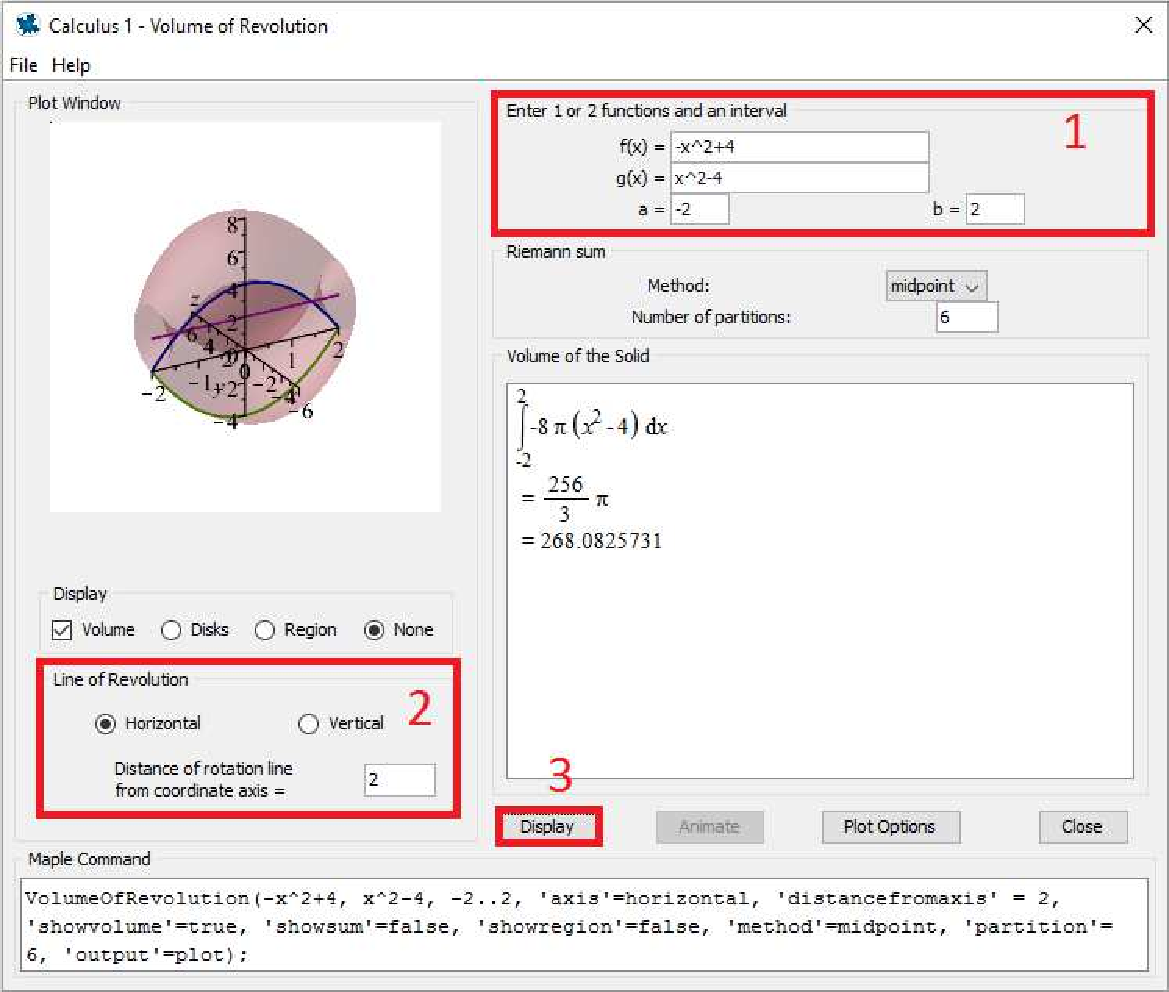
\includegraphics[width=0.9\textwidth]{tutorials/figures/VoRTutorQ1-1-eps-converted-to.pdf}
\end{figure}

\marginnote[-4cm]{When typing in the functions in the tutor, you will not have access to the palettes toolbar in Maple. You will need to type out commands such as \texttt{sqrt()} for square roots. You must also include the symbol * for multiplication.}

The Maple Command at the bottom of the tutor can be copied and pasted into a new Maple input in your worksheet. You can then change the various options in that command to output the plot of the solid, the integral used to obtain the volume, or the numerical value of the volume.

\begin{maplegroup}
\begin{mapleinput}
\mapleinline{active}{1d}{with(Student[Calculus1]):
}{}
\end{mapleinput}
\end{maplegroup}

\marginnote[1cm]{Using the output from the Volume of Revolution Tutor and changing the \texttt{output} option will let you display the region, the value of the volume, and the integral used to obtain the volume.}

\begin{maplegroup}
\begin{mapleinput}
\mapleinline{active}{1d}{VolumeOfRevolution(-x\symbol{94}2+4, x\symbol{94}2+4, -2..2, 'axis'=horizontal, 'distancefromaxis' = 0, 'showvolume'=true, 'showsum'=false, 'showregion'=false, 'method'=midpoint, 'partition'= 6, 'output'=plot);
}{}
\end{mapleinput}
\mapleresult
%\mapleplot{tutorials/figures/volumeofrevolutionplot3d1-eps-converted-to.pdf}
\mapleplot{tutorials/figures/volumeofrevolutionplot3d1-eps-converted-to.png}
\end{maplegroup}

\begin{maplegroup}
\begin{mapleinput}
\mapleinline{active}{1d}{VolumeOfRevolution(-x\symbol{94}2+4, x\symbol{94}2+4, -2..2, 'axis'=horizontal, 'distancefromaxis' = 0, 'showvolume'=true, 'showsum'=false, 'showregion'=false, 'method'=midpoint, 'partition'= 6, 'output'=integral);
}{}
\end{mapleinput}
\mapleresult
\begin{maplelatex}
\mapleinline{inert}{2d}{Int(16*Pi*x^2, x = -2 .. 2)}{\[\displaystyle \int_{-2}^{2}\!16\,\pi\,{x}^{2}\,{\rm d}x\]}
\end{maplelatex}
\end{maplegroup}

\index{volume of revolution!tutor}

\begin{maplegroup}
\begin{mapleinput}
\mapleinline{active}{1d}{VolumeOfRevolution(-x\symbol{94}2+4, x\symbol{94}2+4, -2..2, 'axis'=horizontal, 'distancefromaxis' = 0, 'showvolume'=true, 'showsum'=false, 'showregion'=false, 'method'=midpoint, 'partition'= 6, 'output'=value);
}{}
\end{mapleinput}
\mapleresult
\begin{maplelatex}
\mapleinline{inert}{2d}{(256/3)*Pi}{\[\displaystyle {\frac {256\,\pi}{3}}\]}
\end{maplelatex}
\end{maplegroup}

\clearpage

\subsection{Volume Obtained by Rotating the Region Bounded by the Parabolas $y=x^2-4$ and $y=-x^2+4$ about $x=-3$}

In this case, we will revolve the same region as above, but around a vertical axis.

\index{volume of revolution!tutor}

\begin{figure}
\caption{Setting the Volume of Revolution tutor to revolve the region about a vertical axis.}
\centering
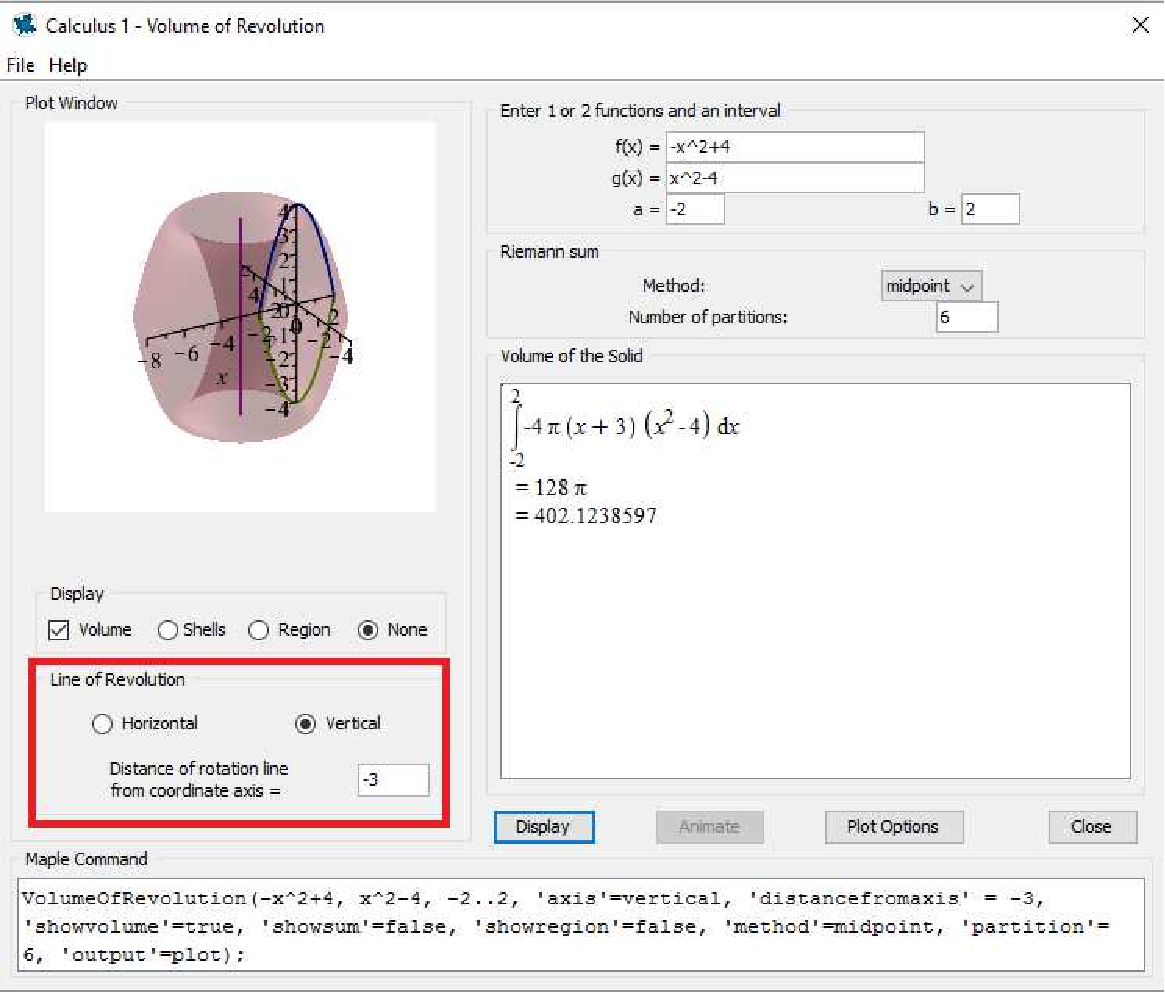
\includegraphics[width=0.9\textwidth]{tutorials/figures/VoRTutorQ1-2-eps-converted-to.pdf}
\end{figure}

\section{Arc Length}
\label{sec:arc_length}
We can use the \texttt{ArcLength()} command that is available in the \texttt{Student[Calculus1]} package to find the arc length of a function over a specified interval.

\index{packages!Student[Calculus1]}
\index{arc length}
\index{evalf}

\subsection{Arc Length of a Parabola}

\begin{maplegroup}
\begin{mapleinput}
\mapleinline{active}{1d}{with(Student[Calculus1]):
}{}
\end{mapleinput}
\end{maplegroup}

\begin{maplegroup}
\begin{mapleinput}
\mapleinline{active}{1d}{g(x) := x\symbol{94}2;
}{}
\end{mapleinput}
\mapleresult
\begin{maplelatex}
\mapleinline{inert}{2d}{g := proc (x) options operator, arrow; x^2 end proc}{\[\displaystyle g\, := \,x\mapsto {x}^{2}\]}
\end{maplelatex}
\end{maplegroup}

\begin{maplegroup}
\begin{mapleinput}
\mapleinline{active}{1d}{arcg := ArcLength(g(x), x=0..Pi);
}{}
\end{mapleinput}
\mapleresult
\begin{maplelatex}
\mapleinline{inert}{2d}{arcg := (1/2)*Pi*sqrt(4*Pi^2+1)-(1/4)*ln(-2*Pi+sqrt(4*Pi^2+1))}{\[\displaystyle {\it arcg}\, := \,1/2\,\pi \, \sqrt{4\,{\pi }^{2}+1}-1/4\,\ln  \left( -2\,\pi + \sqrt{4\,{\pi }^{2}+1} \right) \]}
\end{maplelatex}
\end{maplegroup}

\begin{maplegroup}
\begin{mapleinput}
\mapleinline{active}{1d}{evalf(arcg);
}{}
\end{mapleinput}
\mapleresult
\begin{maplelatex}
\mapleinline{inert}{2d}{10.62814707}{\[\displaystyle  10.62814707\]}
\end{maplelatex}
\end{maplegroup}
\clearpage

\subsection{Arc Length of a Sinusoid}

\index{mathematical functions!sine}

\begin{maplegroup}
\begin{mapleinput}
\mapleinline{active}{1d}{f(x) := sin(x);
}{}
\end{mapleinput}
\mapleresult
\begin{maplelatex}
\mapleinline{inert}{2d}{f := proc (x) options operator, arrow; sin(x) end proc}{\[\displaystyle f\, := \,x\mapsto \sin \left( x \right) \]}
\end{maplelatex}
\end{maplegroup}

\begin{maplegroup}
\begin{mapleinput}
\mapleinline{active}{1d}{arcf := ArcLength(f(x), x=0..Pi);
}{}
\end{mapleinput}
\mapleresult
\marginnote{\texttt{EllipticE()} is a special function in Maple that you don't have to know. We at least can evaluate it, however.}
\begin{maplelatex}
\mapleinline{inert}{2d}{arcf := 2*sqrt(2)*EllipticE((1/2)*sqrt(2))}{\[\displaystyle {\it arcf}\, := \,2\, \sqrt{2}{\it EllipticE} \left( 1/2\, \sqrt{2} \right) \]}
\end{maplelatex}
\end{maplegroup}

\begin{maplegroup}
\begin{mapleinput}
\mapleinline{active}{1d}{evalf(arcf);
}{}
\end{mapleinput}
\mapleresult
\begin{maplelatex}
\mapleinline{inert}{2d}{3.820197788}{\[\displaystyle  3.820197788\]}
\end{maplelatex}
\end{maplegroup}

\index{arc length}
\index{evalf}
\index{arc length!output=integral}


We can add the parameter \texttt{output = integral} to the \texttt{ArcLength()} command to display the integral for calculating the arc length.

\begin{maplegroup}
\begin{mapleinput}
\mapleinline{active}{1d}{ArcLength(f(x), x=0..Pi, output=integral);
}{}
\end{mapleinput}
\mapleresult
\begin{maplelatex}
\mapleinline{inert}{2d}{Int(sqrt(cos(x)^2+1), x = 0 .. Pi)}{\[\displaystyle \int _{0}^{\pi }\! \sqrt{ \left( \cos \left( x \right)  \right) ^{2}+1}\,\,{dx}\]}
\end{maplelatex}
\end{maplegroup}

\chapter{Differential Equations}
\label{chp:differential_equations}						

We want to find solutions (and potentially graph said solutions) of \textbf{differential equations} -- equations that contain functions and derivatives of these functions. For the sake of ease, we will look at \textbf{first-order differential equations}: differential equations that only contain the \textbf{first} derivative (no higher-order derivatives).

\section{Finding the General Solution to a Differential Equation}
\label{sec:finding_general_solution_to_DE}

As an example, let's consider the differential equation $$y'=x^2y,$$ which is a first-order differential equation, where we assume $y$ is a function of $x$. The goal is to find the function $y(x)$ that satisfies this equation. \\

When we define differential equations in Maple, we must ensure that we write $y$ in function notation; this means we write it as $y(x)$ and not as $y$.

\begin{maplegroup}
\begin{mapleinput}
\mapleinline{active}{1d}{de1 := y'(x)= x\symbol{94}2*y(x);
}{}
\end{mapleinput}
\mapleresult
\begin{maplelatex}
\mapleinline{inert}{2d}{de1 := y'(x) = x^2*y(x)}{\[\displaystyle {\it de1}\, := \,{\frac {d}{dx}}y \left( x \right) ={x}^{2}y \left( x \right) \]}
\end{maplelatex}
\end{maplegroup}

We use the \texttt{dsolve()} command to solve a differential equation.

\index{assignment operator!differential equations}
\index{differential equations!dsolve}

\begin{maplegroup}
\begin{mapleinput}
\mapleinline{active}{1d}{dsolve(de1, y(x));
}{}
\end{mapleinput}
\marginnote[-0.5cm]{A package does not need to be imported to use the \texttt{dsolve()} command.}
\mapleresult
\begin{maplelatex}
\mapleinline{inert}{2d}{y(x) = _C1*exp((1/3)*x^3)}{\[\displaystyle y \left( x \right) ={\it \_C1}\,{{\rm e}^{1/3\,{x}^{3}}}\]}
\end{maplelatex}
\end{maplegroup}

\noindent
Note that the result has $\_C1$ as the coefficient. This is an arbitrary constant that is part of the solution of the differential equation. By default, Maple names the constants $\_C1, \_C2, \_C3, \ldots \text{ etc}$.\\

We can clean this up a bit by substituting a `nicer' constant for $\_C1$.

\index{subs}
\index{differential equations!dsolve!general solution}

\begin{maplegroup}
	\begin{mapleinput}
		\mapleinline{active}{1d}{desoln := subs(_C1=A, _C1*exp((1/3)*x^3));
		}{}
	\end{mapleinput}
	\mapleresult
	\begin{maplelatex}
		\mapleinline{inert}{2d}{desoln := A*exp((1/3)*x^3)}{\[\displaystyle desoln :={\it A}\,{{\rm e}^{1/3\,{x}^{3}}}\]}
	\end{maplelatex}
\end{maplegroup}

\noindent
This solution with the arbitrary constant $A$, is known as the \textbf{general solution} to the differential equation.

\section{Finding the Particular Solution given Initial Conditions}
\label{sec:finding_particular_solution_given_IC}

\index{differential equations!dsolve!particular solution}
\index{differential equations!dsolve!initial condition}

The constant $A$ from the above example is arbitrary, meaning that the function $y(x)=A{\rm e}^{1/3\,{x}^{3}}$ is always a solution for the original differential equation, no matter the value of $A$.\\

If we are given an \textbf{initial condition} of the form $y(x_0)=y_0$ for constants $x_0$ and $y_0$, then we can find a unique solution for the differential equation. This will give us a new value for $A$ every time we change the initial condition.

For example, suppose that the function $y(x)$ goes through the point $(0,5)$. In this case, we have the initial condition $y(0)=5$.

To include this initial condition when solving the differential equation in Maple, we add it into the \texttt{dsolve()} command as follows:
\begin{maplegroup}
\begin{mapleinput}
\mapleinline{active}{1d}{dsolve([de1, y(0) = 5], y(x));
}{}
\end{mapleinput}

\mapleresult
\begin{maplelatex}
\mapleinline{inert}{2d}{y(x) = 5*exp((1/3)*x^3)}{\[\displaystyle y \left( x \right) =5\,{{\rm e}^{1/3\,{x}^{3}}}\]}
\end{maplelatex}
\marginnote[-0.5cm]{The particular solution to $y'=x^2y$ with the initial condition $y(0)=5$ is $y \left( x \right) =5\,{{\rm e}^{1/3\,{x}^{3}}}$.}
\end{maplegroup}

\section{Direction Fields}
\label{sec:direction_fields_tutorial}

\index{packages!DETools}

A direction field is a way to plot an entire family of solutions on a graph. Each arrow on this direction field represents the slope of the tangent line at every point in the graph's range. To access this command, we need to import the \texttt{DETools} package.

\begin{maplegroup}
\begin{mapleinput}
\mapleinline{active}{1d}{with(DETools):
}{}
\end{mapleinput}
\end{maplegroup}
\marginnote[-0.3cm]{The \texttt{DETools} package must be loaded to use the \texttt{DEplot()} command.}

\index{mathematical functions!sine}

\begin{maplegroup}
\begin{mapleinput}
\mapleinline{active}{1d}{de2 := y'(x) = x\symbol{94}2 * sin(y(x));
}{}
\end{mapleinput}
\mapleresult
\marginnote[0.5cm]{This differential equation may be written as $y'=x^2\sin(y)$.}
\begin{maplelatex}
\mapleinline{inert}{2d}{de2 := y'(x) = x^2*sin(y(x))}{\[\displaystyle {\it de2}\, := \,{\frac {d}{dx}}y \left( x \right) ={x}^{2}\sin \left( y \left( x \right)  \right) \]}
\end{maplelatex}
\end{maplegroup}

We can use \texttt{DEplot()} to plot the direction field for the differential equation. The required parameters for the \texttt{DEplot()} command are the differential equation, the function for which it is to be solved for, and the ranges of the two variables.

\index{differential equations!DEplot}

\begin{maplegroup}
\begin{mapleinput}
\mapleinline{active}{1d}{DEplot(de2, y(x), x=-2..2, y=-2..2);
}{}
\end{mapleinput}
\mapleresult
\mapleplot{tutorials/figures/direction_fieldsplot2d1-eps-converted-to.pdf}
\end{maplegroup}

The above direction field allows us to track a "solution curve" for any particular initial condition. To track this curve, we start at a point $(x_0, y_0)$ and follow the directions of the arrows. This will give us the \textbf{one} unique curve that satisfies the initial condition $y(x_0)=y_0$. 

\marginnote{Square brackets must be placed around the initial condition of a particular solution when plotting a solution curve.}
Maple will plot a particular solution if the initial condition is placed inside square brackets and included as an additional parameter in the \texttt{DEplot()} command.

\subsection{Plotting Solution Curves on a Direction Field}

\index{differential equations!DEplot!axes intervals}
\index{differential equations!DEplot!solution curves}
\index{differential equations!DEplot!linecolour}

If we want to force the \texttt{DEplot()} command to show a solution for one particular initial condition, say $y(0)=1$, we add the parameter as follows:

\begin{maplegroup}
\begin{mapleinput}
\mapleinline{active}{1d}{DEplot(de2, y(x), x=-2..2, y=-2..2, [y(0) = 1]);
}{}
\end{mapleinput}
\mapleresult
\mapleplot{tutorials/figures/direction_fieldsplot2d2-eps-converted-to.pdf}
\end{maplegroup}
\marginnote[-2cm]{Notice that this curve goes through the point $(0,1)$ and follows the direction of the arrows from the direction field.}

We now plot the solutions that correspond to the initial conditions $y(0)=1$ and $y(2)=-1$:

\begin{maplegroup}
\begin{mapleinput}
\mapleinline{active}{1d}{DEplot(de2, y(x), x=-2..2, y=-2..2, [y(0) = 1, y(2) = -1], linecolour=[blue, cyan]);
}{}
\end{mapleinput}
\mapleresult
\mapleplot{tutorials/figures/direction_fieldsplot2d3-eps-converted-to.pdf}
\end{maplegroup}

\marginnote[-2cm]{The \texttt{linecolour = }\textit{colour} parameter is used to adjust the colour of the solution curves, rather than the direction field.}
\chapter{Sequences and Series}
\label{chp:sequence_and_sseries}			

Suppose we want to generate a list of integers that are $2$ more than a multiple of $3$. For example, $32$ is one of these numbers because $32 = 3(10)+2$. In other words, we want to create a list of numbers of the form $3k+2$. \\

\index{sequences and series}

Or perhaps we want a nice way to express and generate all the odd numbers $1,3,5,7,9,\ldots$ (numbers of the form $2k+1$).\\

These lists are called \textit{sequences}. In both of these examples, $k$ is known as an \textit{index}.

\section{Sequences using \$ Notation}
\label{sec:sequences_using_dollar_notation}
\index{sequences and series!\$ notation}

The shortest way to list the terms in a sequence is using the \$ symbol. 

\begin{maplegroup}
\begin{mapleinput}
\mapleinline{active}{1d}{3*k\symbol{94}2+2 \$ k=0..3;
}{}
\end{mapleinput}
\marginnote{The notation for these sequences is \[\displaystyle\left(3k^2+2\right)_{k=0}^3\] and \[\displaystyle\left(2k^2-k\right)_{k=1}^5.\]}
\mapleresult
\begin{maplelatex}
\mapleinline{inert}{2d}{2, 5, 14, 29}{\[\displaystyle 2,\,5,\,14,\,29\]}
\end{maplelatex}
\end{maplegroup}

\noindent Now let's generate five integers of the form $2k^2-k$:

\begin{maplegroup}
\begin{mapleinput}
\mapleinline{active}{1d}{2*k\symbol{94}2-k \$ k=1..5;
}{}
\end{mapleinput}
\mapleresult
\begin{maplelatex}
\mapleinline{inert}{2d}{1, 6, 15, 28, 45}{\[\displaystyle 1,\,6,\,15,\,28,\,45\]}
\end{maplelatex}
\end{maplegroup}

\section{Sequences using the \texttt{seq()} Command}
\label{sec:sequences_using_the_seq_command}

We can also list the terms in a sequence by using the \texttt{seq()} command. This command essentially performs the same operation as the \$ symbol from the previous section.

\index{sequences and series!seq}

\begin{maplegroup}
\begin{mapleinput}
\mapleinline{active}{1d}{seq(2*k\symbol{94}2-k, k=1..5);
}{}
\end{mapleinput}
\marginnote{The sequence $\displaystyle\left(2k^2-k\right)_{k=1}^5$.}
\mapleresult
\begin{maplelatex}
\mapleinline{inert}{2d}{1, 6, 15, 28, 45}{\[\displaystyle 1,\,6,\,15,\,28,\,45\]}
\end{maplelatex}
\end{maplegroup}

\section{Defining and Evaluating Series}
\label{sec:defining_and_evaluating_series}

We use the capitalized \texttt{Sum()} command to display the summation notation for a series symbolically. This also makes it possible to assign a name to the sum and use it in other commands later.

Much like with sequences, we need a generating function involving an index, such as $k$. We then specify the range of indices for the terms in that sequence that are to be summed.

\marginnote[0.5cm]{This is a called a \textit{finite} sum, since only finitely many terms are summed.}
\begin{maplegroup}
\begin{mapleinput}
\mapleinline{active}{1d}{s1 := Sum(2*k\symbol{94}2-k, k=1..5);
}{}
\end{mapleinput}
\mapleresult
\begin{maplelatex}
\mapleinline{inert}{2d}{s1 := Sum(2*k^2-k, k = 1 .. 5)}{\[\displaystyle {\it s1}\, := \,\sum _{k=1}^{5}2\,{k}^{2}-k\]}
\end{maplelatex}
\end{maplegroup}

\index{sequences and series!Sum}

We use the lowercase \texttt{sum()} command to calculate the value of the sum. We may also use the \texttt{value()} command on the result of a capitalized \texttt{Sum()} command.

\begin{maplegroup}
\begin{mapleinput}
\mapleinline{active}{1d}{value(s1);
}{}
\end{mapleinput}
\mapleresult
\begin{maplelatex}
\mapleinline{inert}{2d}{95}{\[\displaystyle 95\]}
\end{maplelatex}
\end{maplegroup}

\begin{maplegroup}
\begin{mapleinput}
\mapleinline{active}{1d}{sum(2*k\symbol{94}2-k, k=1..5);
}{}
\end{mapleinput}
\mapleresult
\begin{maplelatex}
\mapleinline{inert}{2d}{95}{\[\displaystyle 95\]}
\end{maplelatex}
\end{maplegroup}

\index{value}
\index{sequences and series!sum}

To determine the value of the sum of infinitely many terms, we can use \texttt{infinity} as the a bound on the index. The value of an infinite sum may be a value (in the case of a convergent sum) or $\pm\infty$ (in the case of a divergent sum).

\begin{maplegroup}
\begin{mapleinput}
\mapleinline{active}{1d}{s2 := Sum((2/3)\symbol{94}k, k=0..infinity);
}{}
\end{mapleinput}
\marginnote[0.5cm]{The infinite sum $\displaystyle\sum_{k=0}^{\infty} \left(\dfrac{2}{3}\right)^k$ is said to be convergent.}
\mapleresult
\begin{maplelatex}
\mapleinline{inert}{2d}{s2 := Sum((2/3)^k, k = 0 .. infinity)}{\[\displaystyle {\it s2}\, := \,\sum _{k=0}^{\infty } \left( 2/3 \right) ^{k}\]}
\end{maplelatex}
\end{maplegroup}

\begin{maplegroup}
\begin{mapleinput}
\mapleinline{active}{1d}{value(s2);
}{}
\end{mapleinput}
\mapleresult
\begin{maplelatex}
\mapleinline{inert}{2d}{3}{\[\displaystyle 3\]}
\end{maplelatex}
\end{maplegroup}

\begin{maplegroup}
\begin{mapleinput}
\mapleinline{active}{1d}{s3 := Sum(sin(k)+1, k=1..infinity);
}{}
\end{mapleinput}
\marginnote[0.5cm]{The infinite sum $\,\,\,\,\displaystyle\sum_{k=1}^{\infty} (\sin(k)+1)$ is said to be divergent.}
\mapleresult
\begin{maplelatex}
\mapleinline{inert}{2d}{s3 := Sum(sin(k)+1, k = 1 .. infinity)}{\[\displaystyle {\it s3}\, := \,\sum _{k=1}^{\infty }\sin \left( k \right) +1\]}
\end{maplelatex}
\end{maplegroup}

\index{mathematical functions!sine}
\index{sequences and series!infinite series}

\begin{maplegroup}
\begin{mapleinput}
\mapleinline{active}{1d}{value(s3);
}{}
\end{mapleinput}
\mapleresult
\begin{maplelatex}
\mapleinline{inert}{2d}{infinity}{\[\displaystyle \infty \]}
\end{maplelatex}
\end{maplegroup}

\section{Taylor and Maclaurin Series}
\label{sec:taylor_and_maclaurin_series}

\index{sequences and series!Taylor and Maclaurin series}

One use of series is to find the Taylor series expansion of a function. Recall that the Taylor series of a function $f(x)$, centred at $x=a$, is the sum 
\begin{equation*}
\sum_{k=0}^{\infty} \dfrac{f^{(k)}(a)}{n!}(x-a)^k.
\end{equation*}
A Taylor series that is centred at $x=0$ is known as a Maclaurin series.

\subsection{Maclaurin Series Expansion of ${\rm e}^x$}

\index{mathematical functions!exponential}
\index{sequences and series!Taylor and Maclaurin series!taylor}

\marginnote[0.5cm]{Maple has given $7$ terms as an output. The $O(x^6)$ term in this expression means "plus a bunch more terms with power $6$ and higher".}
\begin{maplegroup}
\begin{mapleinput}
\mapleinline{active}{1d}{taylor(exp(x), x = 0);
}{}
\end{mapleinput}
\mapleresult
\begin{maplelatex}
\mapleinline{inert}{2d}{1+x+(1/2)*x^2+(1/6)*x^3+(1/24)*x^4+(1/120)*x^5+O(x^6)}{\[\displaystyle 1+x+\frac{1}{2}\,{x}^{2}+\frac{1}{6}\,{x}^{3}+\frac{1}{24}\,{x}^{4}+\frac{1}{120}\,{x}^{5}+O \left( {x}^{6} \right) \]}
\end{maplelatex}
\end{maplegroup}

We can specify the order (related to number of terms) of the Taylor series by adding a number as the final argument to the command.

\begin{maplegroup}
\begin{mapleinput}
\mapleinline{active}{1d}{taylor(exp(x), x = 0, 10);
}{}
\end{mapleinput}
\mapleresult
\begin{maplelatex}
\mapleinline{inert}{2d}{1+x+(1/2)*x^2+(1/6)*x^3+(1/24)*x^4+(1/120)*x^5+(1/720)*x^6+(1/5040)*x^7+(1/40320)*x^8+(1/362880)*x^9+O(x^10)}
{\[\begin{array}{l}\displaystyle 1+x+\frac{1}{2}\,{x}^{2}+\frac{1}{6}\,{x}^{3}+\frac{1}{24}\,{x}^{4}+\frac{1}{120}\,{x}^{5}\\
\displaystyle +{\frac {1}{720}}\,{x}^{6}+{\frac {1}{5040}}\,{x}^{7}+{\frac {1}{40320}}\,{x}^{8}+{\frac {1}{362880}}\,{x}^{9}+O \left( {x}^{10} \right) \end{array}\]}
\end{maplelatex}
\end{maplegroup}
\marginnote[-1cm]{In this example, Maple has displayed all the terms with powers less than $10$.}

\subsection{Taylor Series Expansion of $\sin(x)$, Centred at $x=5$}

\index{sequences and series!Taylor and Maclaurin series!taylor}
\index{mathematical functions!sine}

\begin{maplegroup}
\begin{mapleinput}
\mapleinline{active}{1d}{taylor(sin(x), x = 5, 4);
}{}
\end{mapleinput}
\mapleresult
\begin{maplelatex}
\mapleinline{inert}{2d}{sin(5)+cos(5)*(x-5)-(1/2)*sin(5)*(x-5)^2-(1/6)*cos(5)*(x-5)^3+O((x-5)^4)}
{\[\begin{array}{l}\displaystyle \sin \left( 5 \right) +\cos \left( 5 \right)  \left( x-5 \right) -\frac{1}{2}\,\sin \left( 5 \right)  \left( x-5 \right) ^{2}\\
\displaystyle -\frac{1}{6}\,\cos \left( 5 \right)  \left( x-5 \right) ^{3}+O \left(  \left( x-5 \right) ^{4} \right) \end{array} \]}
\end{maplelatex}
\end{maplegroup}

\subsection{Comparing the Graphs of $\sin(x)$ and its Maclaurin Series}

We can see how closely the Maclaurin (or Taylor) series expansion resembles the original function by plotting them on the same axes. To plot the Taylor series we need to get rid of the final term $O(\ldots)$. We use the \texttt{convert()} command to do this.

\index{sequences and series!Taylor and Maclaurin series!convert to polynomial}
\index{ditto operator}
\index{plot!axes intervals}
\index{plot!multiple functions}

\marginnote[0.5cm]{This \texttt{convert()} command lets Maple know that we wish for the result to be a truncated polynomial.}
\begin{maplegroup}
\begin{mapleinput}
\mapleinline{active}{1d}{taylor(sin(x), x = 0, 10); poly := convert(%, polynom);
}{}
\end{mapleinput}
\mapleresult
\begin{maplelatex}
\mapleinline{inert}{2d}{x-(1/6)*x^3+(1/120)*x^5-(1/5040)*x^7+(1/362880)*x^9+O(x^11)}{\[\displaystyle x-\frac{1}{6}\,{x}^{3}+{\frac {1}{120}}\,{x}^{5}-{\frac {1}{5040}}\,{x}^{7}+{\frac {1}{362880}}\,{x}^{9}+O \left( {x}^{11} \right) \]}
\end{maplelatex}
\begin{maplelatex}
\mapleinline{inert}{2d}{poly := x-(1/6)*x^3+(1/120)*x^5-(1/5040)*x^7+(1/362880)*x^9}{\[\displaystyle {\it poly}\, := \,x-\frac{1}{6}\,{x}^{3}+{\frac {1}{120}}\,{x}^{5}-{\frac {1}{5040}}\,{x}^{7}+{\frac {1}{362880}}\,{x}^{9}\]}
\end{maplelatex}
\end{maplegroup}

\begin{maplegroup}
\begin{mapleinput}
\mapleinline{active}{1d}{plot([sin(x), poly], x = -4*Pi..4*Pi, y = -10..10);
}{}
\end{mapleinput}
\mapleresult
\mapleplot{tutorials/figures/Taylor_and_Maclaurin_Seriesplot2d1-eps-converted-to.pdf}
\end{maplegroup}
\chapter{Conditional Statements and Loops}
\label{chp:conditional_statements_and_loops}	

\section{\texttt{if}/\texttt{else} Statements}

\index{conditional statements!if/else statements}

`If' and `else' statements allow us to test various conditions. The result then changes based on whether the given condition is \textbf{true} or \textbf{false}.\\

For example, let's say that someone makes the statement\\
\begin{center} \textit{"If it's sunny tomorrow, then I will go for a bike ride."} \end{center}

If it is, in fact, sunny tomorrow, then that person \textbf{will} go for a bike ride. In other words, since the "sunny tomorrow" condition becomes TRUE, then the following implication "go for a bike ride" will happen.\\

As the statement stands now, we have no idea what this person will do if it is \textbf{not} sunny. Perhaps they will still go for a bike ride, perhaps not. We can define this action with an `else' statement.\\

In other words, we can define what will happen if it is \textbf{not sunny}. For example:\\
\begin{center} \textit{"If it's sunny tomorrow, then I will go for a bike ride. Otherwise, I will read a book at home."} \end{center}

\noindent
From this example, we know that the following are true.
\begin{itemize}
	\item If it's sunny tomorrow, then I will go for a bike ride.
	\item If it's not sunny tomorrow, then I read a book at home.
\end{itemize}

\subsection{A Conditional Statement based on Numerical Value}

We will outline this concept with a silly example. We define two variables $a=2$ and $b=5$. If $a<b$ is \textbf{true} (which it is because obviously $2$ is less than $5$), we print the word "Mario". Otherwise (if it's \textbf{false}), we print the word "Luigi". Therefore, we expect that "Mario" will be printed.
\begin{maplegroup}
\begin{mapleinput}
\begin{verbatim}
> a := 2: b := 5:
> if a < b then
    print("Mario")
  else
    print("Luigi")
  end if
\end{verbatim}
\end{mapleinput}
\mapleresult
\begin{maplelatex}
\mapleinline{inert}{2d}{"Mario"}{\[\displaystyle \text{``Mario''}\]}
\end{maplelatex}
\end{maplegroup}
\marginnote[-1.5cm]{You can use Shift+Enter to create multiple lines within the same Maple input.}

\subsection{A Conditional Statement to Check Even/Odd}

Now we consider a more useful example. We define a function $f(x)$ and check whether substituting $x=2$ into this function outputs an \textbf{even} number or an \textbf{odd} number. 

\begin{maplegroup}
\begin{mapleinput}
\begin{verbatim}
> f(x) := x^2 + 3*x - 4:
> if type(f(2), even) then
    print(f(2), "even")
  else
    print(f(2), "odd")
  end if
\end{verbatim}
\end{mapleinput}
\marginnote[-1.5cm]{The \texttt{type()} command is used to check if the expression has the specified property.}
\mapleresult
\begin{maplelatex}
\mapleinline{inert}{2d}{6, "even"}{\[\displaystyle 6,\,\text{``even''}\]}
\end{maplelatex}
\end{maplegroup}

\subsection{A Conditional Statement to Check if a Limit Exists}

\index{conditional statements!if/else statements}
\index{limit}

We define a function $f(x)$ and then use an `if' statement to verify whether or not the limit of $f(x)$ as $x$ approaches $0$ is \textit{numeric}. In other words, we are checking to see whether or not this limit exists.

\begin{maplegroup}
\begin{mapleinput}
\begin{verbatim}
> f(x) := 1/x:
> L := limit(f(x), x=0):
> if type(L, numeric) then
    print("Limit is defined")
  else
    print("Limit is undefined")
  end if
\end{verbatim}
\end{mapleinput}
\mapleresult
\marginnote[-1cm]{Does $\displaystyle\lim_{x \to 0} \dfrac{1}{x}$ exist? Does the limit give a number $L$ as a result, or something that is \textbf{not} a number?}
\begin{maplelatex}
\mapleinline{inert}{2d}{"Limit is undefined"}{\[\displaystyle \text{``Limit is undefined''}\]}
\end{maplelatex}
\end{maplegroup}

\section{\texttt{if}/\texttt{elif}/\texttt{else} Statements}

\index{conditional statements!if/elif/else statements}

The \texttt{elif} (else if) command allows us to add more than one condition to our statement. For example, if we want to test whether a particular number is (i) positive, (ii) negative, or (iii) zero, and wish to have different outputs based on these \textbf{three} possibilities, we can do so with a combination of \texttt{if}, \texttt{else}, and \texttt{elif}.\\

\subsection{Using Conditional Statements to Interpret the First Derivative}
In this example, we will use one of these statements to illustrate the first derivative test in calculus. We would like to answer the following question: for a particular value $x=a$, is the function $g(x)$ (i) increasing (positive derivative), (ii) decreasing (negative derivative), or (iii) neither increasing nor decreasing (zero derivative)?

\begin{maplegroup}
\begin{mapleinput}
\begin{verbatim}
> g(x) := x^4 - 4*x^3 + 3*x^2:
> a := 0:
> if subs(x = a, diff(g(x), x)) > 0 then
    print("increasing")
  elif subs(x = a, diff(g(x), x)) < 0 then
    print("decreasing")
  else print("neither")
  end if
\end{verbatim}
\end{mapleinput}
\mapleresult
\begin{maplelatex}
\mapleinline{inert}{2d}{"neither"}{\[\displaystyle \text{``neither''}\]}
\end{maplelatex}
\end{maplegroup}
\marginnote{This implies that $g'(0)$ is equal to $0$.}

\index{conditional statements!if/elif/else statements}

\section{\texttt{for} Loops}

`For' loops allow us to carry out a computation repeatedly for an entire range of values. We can also combine these loops with conditional statements like `if' and `else'. To use a `for' loop, we are required to type\\

\index{loops!for}

\texttt{for i from a to b do}\\
\hspace{0.5cm}$\cdots$\\
\hspace{0.5cm}$\cdots$\\
\texttt{end do}\\

\noindent
where $i$ is a ``dummy variable", referred to as an index. On the first iteration of the loop, the index begins at $a$. At the end of each iteration, the index is incremented by one. In the last iteration, the index will be equal to $b$.

\subsection{Outputting the First $n$ Derivatives}

We will use a basic `for' loop to output the first $10$ derivatives of the function $f(x)=\sin(2x)$. To do this, we will use the \texttt{diff()} command. The `for' loop will output the $k$\textsuperscript{th} derivative, starting from $k=1$ and ending at $k=10$.
\marginnote{Recall that \texttt{diff(f(x), x\$k)} is the $k$\textsuperscript{th} derivative of $f$ with respect to $x$. Use of the \texttt{diff()} command is explained in Tutorial \ref{chp:derivative}, page \pageref{chp:derivative}.}

\index{mathematical functions!sine}
\index{derivative!diff!higher derivatives}

\begin{maplegroup}
	\begin{mapleinput}
		\begin{verbatim}
		> f(x) := sin(2*x);
		\end{verbatim}
	\end{mapleinput}
	\mapleresult
	\begin{maplelatex}
		\mapleinline{inert}{2d}{f := proc (x) options operator, arrow; sin(2*x) end proc}{\[\displaystyle f\, := \,x\mapsto \sin \left( 2\,x \right) \]}
	\end{maplelatex}
		\begin{mapleinput}
		\begin{verbatim}
		> for k from 1 to 10 do
		     diff(f(x), x$k)
		  end do
		\end{verbatim}
	\end{mapleinput}
	
	\mapleresult
	\begin{maplelatex}
		\mapleinline{inert}{2d}{2*cos(2*x)}{\[\displaystyle 2\,\cos \left( 2\,x \right) \]}
	\end{maplelatex}
	\mapleresult
	\begin{maplelatex}
		\mapleinline{inert}{2d}{-4*sin(2*x)}{\[\displaystyle -4\,\sin \left( 2\,x \right) \]}
	\end{maplelatex}
	\mapleresult
	\begin{maplelatex}
		\mapleinline{inert}{2d}{-8*cos(2*x)}{\[\displaystyle -8\,\cos \left( 2\,x \right) \]}
	\end{maplelatex}
	\mapleresult
	\begin{maplelatex}
		\mapleinline{inert}{2d}{16*sin(2*x)}{\[\displaystyle 16\,\sin \left( 2\,x \right) \]}
	\end{maplelatex}
	\mapleresult
	\begin{maplelatex}
		\mapleinline{inert}{2d}{32*cos(2*x)}{\[\displaystyle 32\,\cos \left( 2\,x \right) \]}
	\end{maplelatex}
	\mapleresult
	\begin{maplelatex}
		\mapleinline{inert}{2d}{-64*sin(2*x)}{\[\displaystyle -64\,\sin \left( 2\,x \right) \]}
	\end{maplelatex}
	\mapleresult
	\begin{maplelatex}
		\mapleinline{inert}{2d}{-128*cos(2*x)}{\[\displaystyle -128\,\cos \left( 2\,x \right) \]}
	\end{maplelatex}
	\mapleresult
	\begin{maplelatex}
		\mapleinline{inert}{2d}{256*sin(2*x)}{\[\displaystyle 256\,\sin \left( 2\,x \right) \]}
	\end{maplelatex}
	\mapleresult
	\begin{maplelatex}
		\mapleinline{inert}{2d}{512*cos(2*x)}{\[\displaystyle 512\,\cos \left( 2\,x \right) \]}
	\end{maplelatex}
	\mapleresult
	\begin{maplelatex}
		\mapleinline{inert}{2d}{-1024*sin(2*x)}{\[\displaystyle -1024\,\sin \left( 2\,x \right) \]}
	\end{maplelatex}
\end{maplegroup}


\subsection{Outputting the Primes up to $50$}

\index{loops!for}
\index{isprime}

Let's say we want to find all of the prime integers from $1$ to $50$. If we enter 
\begin{maplegroup}
	\begin{mapleinput}
		\begin{verbatim}
		> for i from 1 to 50 do
		    print(i);
		  end do
		\end{verbatim}
	\end{mapleinput}
\end{maplegroup}
\marginnote[-1.3cm]{You can use Shift+Enter to create multiple lines within the same Maple input.}
\noindent
into Maple, it will output all the integers from $1$ to $50$, rather than only the prime integers. We include an `if' statement that makes use of the \texttt{isprime()} command to only output primes. 

\begin{maplegroup}
\begin{mapleinput}
\begin{verbatim}
> for i from 1 to 50 do
    if isprime(i) then
      print(i);
    end if
  end do
\end{verbatim}
\end{mapleinput}
\mapleresult
\marginnote[-2cm]{Since we do not want Maple to do anything for a composite integer (an integer that is not prime), we can omit the 'else' component of this 'if' statement.}
\begin{maplelatex}
\mapleinline{inert}{2d}{2}{\[\displaystyle 2\]}
\end{maplelatex}
\mapleresult
\begin{maplelatex}
\mapleinline{inert}{2d}{3}{\[\displaystyle 3\]}
\end{maplelatex}
\mapleresult
\begin{maplelatex}
\mapleinline{inert}{2d}{5}{\[\displaystyle 5\]}
\end{maplelatex}
\mapleresult
\begin{maplelatex}
\mapleinline{inert}{2d}{7}{\[\displaystyle 7\]}
\end{maplelatex}
\mapleresult
\begin{maplelatex}
\mapleinline{inert}{2d}{11}{\[\displaystyle 11\]}
\end{maplelatex}
\mapleresult
\begin{maplelatex}
\mapleinline{inert}{2d}{13}{\[\displaystyle 13\]}
\end{maplelatex}
\mapleresult
\begin{maplelatex}
\mapleinline{inert}{2d}{17}{\[\displaystyle 17\]}
\end{maplelatex}
\mapleresult
\begin{maplelatex}
\mapleinline{inert}{2d}{19}{\[\displaystyle 19\]}
\end{maplelatex}
\begin{maplelatex}
	\mapleinline{inert}{2d}{...}{\[\vdots\]}
\end{maplelatex}
\end{maplegroup}

\section{\texttt{for}/\texttt{while} Loops}

\index{loops!while}

Adding a `while' is a short way of adding an inherent `if' for every value of the `for' loop. In the next example, we add \texttt{`while i\symbol{94}2 < 100'} to check that the square of the index $i$ is less than $100$ every time it increases in value. The moment that this condition is no longer met, the loop terminates.

Let's say we want to add the first few squares together: $1^2+2^2+3^2+\cdots$ until $i^2$ becomes greater than or equal to $100$. Instead of adding an `if' statement every time the loop increases, we can do the same thing with a `while':

\marginnote{We assign an initial total of $0$ so that we can add a value to it for each iteration of the loop. 
    \texttt{total := total + i}\string^\texttt{2}
	adds $i^2$ to the current value of \texttt{total} before reassigning the new value.}
\begin{maplegroup}
\begin{mapleinput}
\begin{verbatim}
> total := 0:
> for i from 1 while i^2 < 100 do
    total := total + i^2
  end do
\end{verbatim}
\end{mapleinput}
\mapleresult
\begin{maplelatex}
\mapleinline{inert}{2d}{total := 1}{\[\displaystyle {\it total}\, := \,1\]}
\end{maplelatex}
\mapleresult
\begin{maplelatex}
\mapleinline{inert}{2d}{total := 5}{\[\displaystyle {\it total}\, := \,5\]}
\end{maplelatex}
\mapleresult
\begin{maplelatex}
\mapleinline{inert}{2d}{total := 14}{\[\displaystyle {\it total}\, := \,14\]}
\end{maplelatex}
\mapleresult
\begin{maplelatex}
\mapleinline{inert}{2d}{total := 30}{\[\displaystyle {\it total}\, := \,30\]}
\end{maplelatex}
\mapleresult
\begin{maplelatex}
\mapleinline{inert}{2d}{total := 55}{\[\displaystyle {\it total}\, := \,55\]}
\end{maplelatex}
\mapleresult
\begin{maplelatex}
\mapleinline{inert}{2d}{total := 91}{\[\displaystyle {\it total}\, := \,91\]}
\end{maplelatex}
\mapleresult
\begin{maplelatex}
\mapleinline{inert}{2d}{total := 140}{\[\displaystyle {\it total}\, := \,140\]}
\end{maplelatex}
\mapleresult
\begin{maplelatex}
\mapleinline{inert}{2d}{total := 204}{\[\displaystyle {\it total}\, := \,204\]}
\end{maplelatex}
\mapleresult
\begin{maplelatex}
\mapleinline{inert}{2d}{total := 285}{\[\displaystyle {\it total}\, := \,285\]}
\end{maplelatex}
\end{maplegroup}
\begin{Maple Normal}{
\begin{Maple Normal}{
\mapleinline{inert}{2d}{}{\[\displaystyle \]}
}\end{Maple Normal}
}\end{Maple Normal}

\index{loops!while}

 \marginnote[-2cm]{This loop has calculated the value \[1^2+2^2+3^2+4^2+\cdots+7^2+8^2+9^2=285.\]}

\section{\texttt{for} Loops with Conditionals}

We now combine all of the various conditional statements and loops together into one example. Let's assume we have a function $g(x)$ and want to test whether this function is (i) increasing ($g'(x) > 0$), (ii) decreasing ($g'(x) < 0$), or (iii) neither (critical point ($g'(x) = 0$)).

The loop we have constructed behaves according to the following steps:

\index{loops!for}

\begin{enumerate}
	\item Begin with the value $j=-2$.
	\marginnote[-0.3cm]{Note that we can use any letter for the loop index, but the most common choices are $i$, $j$, $k$, and $l$.}
	\item If $g'(j)>0$, then $g$ is increasing at $x=j$.
	\item If $g'(j)<0$, then $g$ is decreasing at $x=j$.
	\item If $g'(j)=0$, then $g$ is neither increasing nor decreasing at $x=j$.
	\item Update $j$ to the next value in the list and repeat steps $2$ through $4$.
\end{enumerate}

\begin{maplegroup}
\begin{mapleinput}
\begin{verbatim}
> g(x) := x^4 - 4*x^3 + 3*x^2:
> for j in [-2, 0, 4] do
    if subs(x = j, diff(g(x), x)) > 0 then
      print(j, "increasing")
    elif subs(x = j, diff(g(x), x)) < 0 then
      print(j, "decreasing")
    else print(j, "neither")
    end if
  end do
\end{verbatim}
\end{mapleinput}
\mapleresult
\begin{maplelatex}
\mapleinline{inert}{2d}{-2, "decreasing"}{\[\displaystyle -2,\,\text{``decreasing''}\]}
\end{maplelatex}
\mapleresult
\begin{maplelatex}
\mapleinline{inert}{2d}{0, "neither"}{\[\displaystyle 0,\,\text{``neither''}\]}
\end{maplelatex}
\mapleresult
\begin{maplelatex}
\mapleinline{inert}{2d}{4, "increasing"}{\[\displaystyle 4,\,\text{``increasing''}\]}
\end{maplelatex}
\end{maplegroup}

\index{conditional statements!if/elif/else statements}
\index{loops!for}

\marginnote[-1cm]{From the output, we an see that $g'(-2) < 0$, $g'(0) = 0$, and $g'(4) > 0$.}


%----------------------------------------------------------------------------------------------%----------------------------------------------------------------------------------------------
\backmatter

% list of common errors
\chapter{List of Common Errors}
\label{chp:list_of_common_errors}

In this section, we will review some of the most common errors encountered when using Maple. Many of these errors are caused when using 2D Math, which makes complicated expressions look pretty, but can cause other issues. For a description of font styles, see Tutorial \ref{chp:maple_environment}, page \pageref{chp:maple_environment}.

\subsection{Missing Brackets}

In Maple, we will use several types of brackets such as parentheses, square brackets, and curly braces. Maple refers to these as delimiters. If these delimiters are not found in pairs, then Maple will be unable to understand the syntax of your command.

\marginnote{In this example, there is an open square bracket, but no square closed bracket.}
\begin{maplegroup}
\begin{mapleinput}
\mapleinline{active}{1d}{plot([f(x), g(x), x =-5..5);}{}
\end{mapleinput}
\mapleresult
\begin{maplelatex}
\mapleinline{inert}{2d}{Error, mismatched or missing bracket/operator}{\texttt{Error, mismatched or missing bracket/operator}}
\end{maplelatex}
\end{maplegroup}

\subsection{Spelling Errors}

Maple cannot correct for poor spelling. If a command is misspelled, then it will treat the command as a variable name.

\marginnote{Maple doesn't know to solve this equation if you don't spell the \texttt{solve()} command properly!}
\begin{maplegroup}
\begin{mapleinput}
\mapleinline{active}{1d}{slove(x^2 = 4);}{}
\end{mapleinput}
\mapleresult
\begin{maplelatex}
\mapleinline{inert}{2d}{slove(x^2 = 4)}{\[\displaystyle {\it slove} \left( {x}^{2}=4 \right) \]}
\end{maplelatex}
\end{maplegroup}

\subsection{The \texttt{\%} Shortcut Not Working as Intended}

The \texttt{\%} shortcut will only use the output command that was last run.

\marginnote{
	In this example, the expected output of the second command is the decimal value of $\cos(\pi)$, which is equal to $-1$. However, it appears that the second command was run after the third, producing the decimal approximation of the third command.
	\par It is usually a good practice to use the \texttt{\%} operator on the same line as the previous command. For example:
	\par 
	\texttt{
	> subs(x=Pi,cos(x)); evalf(\%);
	}
}

\begin{maplegroup}
\begin{mapleinput}
\mapleinline{active}{1d}{subs(x = Pi, cos(x));}{\[> {\it subs}\!\left( x=\pi,\cos \left( x \right)  \right); \]}{}
\end{mapleinput}
\mapleresult
\begin{maplelatex}
\mapleinline{inert}{2d}{cos(Pi)}{\[\displaystyle \cos \left( \pi \right) \]}
\end{maplelatex}
\end{maplegroup}

\begin{maplegroup}
\begin{mapleinput}
\mapleinline{active}{1d}{evalf(%);}{\[> {\it evalf}\!\left(  \% \right); \]}
\end{mapleinput}
\mapleresult
\begin{maplelatex}
\mapleinline{inert}{2d}{.6735930582}{\[\displaystyle  0.6735930582\]}
\end{maplelatex}
\end{maplegroup}

\begin{maplegroup}
\begin{mapleinput}
\mapleinline{active}{1d}{fsolve(x^3 + 4*x = 3);}{\[> {\it fsolve}\!\left( {x}^{3}+4\,x=3 \right); \]}
\end{mapleinput}
\mapleresult
\begin{maplelatex}
\mapleinline{inert}{2d}{.6735930582}{\[\displaystyle  0.6735930582\]}
\end{maplelatex}
\end{maplegroup}

\subsection{Missing Multiplication Between Variables}

Whenever two variables (such as $x$ and $y$) are multiplied together, you must explicitly include the multiplication sign between them. If no * or space is included between the variables, it may be interpreted as an entirely different variable name.

\marginnote{In this example, no multiplication was included between $x$ and $y$. Maple mistakenly thinks that $xy$ is the name of a third variable.}
\begin{maplegroup}
\begin{mapleinput}
\mapleinline{active}{1d}{implicitplot(x^2 + y^2 = 6xy, x =-5..5, y =-5..5);}{\[> {\it implicitplot}(x^2+y^2 = 6xy, x = -5 .. 5, y = -5 .. 5);\]}
\end{mapleinput}
\vspace{.3cm}
\mapleresult
\begin{maplelatex}
\mapleinline{inert}{2d}{}{\texttt{Error, (in plots/implicitplot) invalid input:}}
\mapleinline{inert}{2d}{}{\texttt{the following extra unknowns were found in}}
\mapleinline{inert}{2d}{}{\texttt{the input expression: \{xy\}}}
\end{maplelatex}
\end{maplegroup}

\subsection{Spaces and Parentheses: Multiplication versus Functions}

When typing in 2D Math (the default font), spaces and parentheses may be interpreted by Maple in unintended ways. 

When using commands, make sure that there is no space between the command name and its parentheses. This will be treated as multiplication.

\marginnote{In this example, Maple thinks that the word ``plot" should be multiplied by the expression in parentheses. This is why the name of the command appears in the output.}
\begin{maplegroup}
\begin{mapleinput}
\mapleinline{active}{1d}{plot (x^2 + 5);}{\[> {\it plot} \, \left( {x}^{2}+5 \right); \]}
\end{mapleinput}
\mapleresult
\begin{maplelatex}
\mapleinline{inert}{2d}{plot*(x^2+5)}{\[\displaystyle  {\it plot} \, \left( {x}^{2}+5 \right) \]}
\end{maplelatex}
\end{maplegroup}

Similarly, if there is no space or \texttt{*} between a variable name and the parentheses, the notation may be mistaken as function notation.

\marginnote{Clearly, Maple should be able to expand this basic expression. However, it misinterprets the user's input as being function notation. Maple reads this expression as ``$x$ of $x^3-1$".}
\begin{maplegroup}
\begin{mapleinput}
\mapleinline{active}{1d}{expand(2*x(x^3 - 1));}{\[{\it expand} \left( 2\,x\!\left( {x}^{3}-1 \right)  \right); \]}
\end{mapleinput}
\mapleresult
\begin{maplelatex}
\mapleinline{inert}{2d}{2*x(x^3-1)}{\[\displaystyle 2\,x \left( {x}^{3}-1 \right) \]}
\end{maplelatex}
\end{maplegroup}

\subsection{Assigning Expressions to $x$ or Other Common Variable Names}

It's never a good idea to assign an expression to $x$, $y$, $t$, or other common variable names. If you want to unassign everything at once, you can do this with the \texttt{restart} command on a separate line.

\marginnote{In this example, the value $3$ is assigned to $x$, so the expression $x^2-4x-12$ is equal to the value $-15$. This is remedied after using the \texttt{restart} command.}
\begin{maplegroup}
\begin{mapleinput}
\mapleinline{active}{1d}{x := 3; factor(x^2 - 4x - 12);}{\[> x := 3; \, {\it factor}(x^2-4x-12); \]}
\end{mapleinput}
\mapleresult
\begin{maplelatex}
\mapleinline{inert}{2d}{x := 3}{\[\displaystyle x\, := \,3\]}
\end{maplelatex}
\mapleresult
\begin{maplelatex}
\mapleinline{inert}{2d}{-15}{\[\displaystyle -15\]}
\end{maplelatex}
\end{maplegroup}

\marginnote[1cm]{You will need to load any required packages again after running the \texttt{restart} command.}
\begin{maplegroup}
\begin{mapleinput}
\mapleinline{active}{1d}{restart; factor(x^2 - 4x - 12);}{\[> restart; \, {\it factor}(x^2-4x-12); \]}
\end{mapleinput}
\mapleresult
\begin{maplelatex}
\mapleinline{inert}{2d}{(x+2)*(x-6)}{\[\displaystyle  \left( x+2 \right)  \left( x-6 \right) \]}
\end{maplelatex}
\end{maplegroup}
\clearpage

\subsection{Equals Signs versus Assignment Operator}

The equals sign \texttt{=} must be used for an equation and the assignment operator \texttt{:=} is used to store a value or expression for later use.

\marginnote{The equals sign is used for the \texttt{subs()} command, since we are not assigning the value for the remainder of the document.}
\begin{maplegroup}
\begin{mapleinput}
\mapleinline{active}{1d}{subs(x := 5, cos(x) - 1);}{\[>{\it subs}\!\left(x :=5,\cos \left(x \right)-1\right);\]}
\end{mapleinput}
\mapleresult
\begin{maplelatex}
\mapleinline{inert}{2d}{Error, invalid assignment}{\texttt{Error, invalid assignment}}
\end{maplelatex}
\end{maplegroup}

\subsection{Changing the Order of the Parameters in a Command}

Many commands have multiple parameters and often the order in which the parameters is listed is important. Typing the parameters in an incorrect order in certain commands may cause an error message to be displayed when the command is executed.
\begin{maplegroup}
\begin{mapleinput}
\mapleinline{active}{1d}{subs(4x-3, x=2);}{}
\end{mapleinput}
\vspace{.3cm}
\mapleresult
\begin{maplelatex}
\mapleinline{inert}{2d}{}{\texttt{Error, invalid input: subs received 4x-3,}}
\mapleinline{inert}{2d}{}{\texttt{which is not valid for its 1st argument}}

\end{maplelatex}
\end{maplegroup}
\marginnote[-1.5cm]{In this example, the two parameters in the \texttt{subs()} command need to be interchanged.}

\subsection{Assigning a Function and Not Using Function Notation}

If you have assigned a function (such as $f(x)$) in Maple, make sure to use function notation in other commands, rather than using only the name of the function.

\marginnote{In this example, the \texttt{factor()} command should be \texttt{factor(f(x))}.}
\begin{maplegroup}
\begin{mapleinput}
\mapleinline{active}{1d}{f(x) := x^2 - 4; factor(f);}{\[> f(x) := x^2-4; \, {\it factor}(f);\]}
\end{mapleinput}
\mapleresult
\begin{maplelatex}
\mapleinline{inert}{2d}{f := proc (x) options operator, arrow; x^2-4 end proc}{\[\displaystyle f\, := \,x\mapsto {x}^{2}-4\]}
\end{maplelatex}
\mapleresult
\begin{maplelatex}
\mapleinline{inert}{2d}{f}{\[\displaystyle f\]}
\end{maplelatex}
\end{maplegroup}

\subsection{Case-Sensitive Commands}

Commands are case-sensitive. Make sure to use the correct capitalization.

\marginnote{The correct command here is \texttt{solve()}, which needs a lowercase `s'.}
\begin{maplegroup}
\begin{mapleinput}
\mapleinline{active}{1d}{Solve(3*x + 5 = 2);}{\[> {\it Solve}\!\left( 3\,x+5=2 \right); \]}
\end{mapleinput}
\mapleresult
\begin{maplelatex}
\mapleinline{inert}{2d}{Solve(3*x+5 = 2)}{\[\displaystyle {\it Solve} \left( 3\,x+5=2 \right) \]}
\end{maplelatex}
\end{maplegroup}

There are examples of commands where the capitalized version behaves differently from the non-capitalized version.

\marginnote{In this example, the \texttt{Int()} command and \texttt{int()} command behave differently. Using \texttt{Int()} followed by \texttt{value(\%)} will display the integral and then evaluate it.}
\begin{maplegroup}
\begin{mapleinput}
\mapleinline{active}{1d}{Int(2x, x=10..13);}{\[> {\it Int}(2x, x = 10 .. 13);\]}
\end{mapleinput}
\mapleresult
\begin{maplelatex}
\mapleinline{inert}{2d}{Int(2*x, x = 10 .. 13)}{\[\displaystyle \int_{10}^{13}\!2\,x\,{\rm d}x\]}
\end{maplelatex}
\end{maplegroup}
\begin{maplegroup}
\begin{mapleinput}
\mapleinline{active}{1d}{int(2x, x=10..13);}{\[> {\it int}(2x, x = 10 .. 13);\]}
\end{mapleinput}
\mapleresult
\begin{maplelatex}
\mapleinline{inert}{2d}{69}{\[\displaystyle 69\]}
\end{maplelatex}
\end{maplegroup}

% list of common maple commands
\chapter{List of Common Commands}
\label{chp:list_of_common_commands}

\begin{fullwidth}
%\begin{landscape}
% Table generated by Excel2LaTeX
\begin{longtable}{p{0.33\linewidth} p{0.66\linewidth}}
    \multicolumn{2}{l}{\textbf{Keyboard Shortcuts}} \\
    \hline
    Ctrl+J, Ctrl+K & New execution group (after or before current line) \\
    Ctrl+Shift+J, Ctrl+Shift+K & New  paragraph (after or before current line) \\
    Ctrl+T & Convert line to Paragraph \\
    Ctrl+M & Convert line to Maple input \\
    Ctrl+. & Indent section \\
    Ctrl+, & Unindent section \\
    Ctrl+Delete & Delete section \\
    F4 & Merge consecutive execution groups \\
    F5 & Toggle between Text, Nonexecutable Math, and Math types \\
          &  \\
    \multicolumn{2}{l}{\textbf{Common Expressions}} \\
    \hline
    exp(x) & The exponential function \\
    sqrt(x) & The square root function \\
    abs(x) & The absolute value function \\
    surd(x,n) & The primitive $n$\textsuperscript{th} root, $x^{1/n}$ \\
          &  \\
    \multicolumn{2}{l}{\textbf{Manipulating Expressions}} \\
    \hline
    name := expression & Assigns an expression to a variable \\
    subs(x=a, expression) & Evaluate an expression at $x = a$ \\
    evalf(expression) & Evaluate the given expression as a (floating point) decimal \\
    factor(expression) & Factor the given expression \\
    simplify(expression) & Simplify the given expression \\
    expand(expression) & Expand the given expression \\
    collect(expression,var) & Collect terms of the expression by the specified variable \\
          &  \\
    \multicolumn{2}{l}{\textbf{Solving Equations}} \\
    \hline
    solve(equation,var) & Solves the given equation for the specified variable \\
    fsolve(equation,var) & Solves the given equation for the specified variable (as a decimal) \\
    fsolve(equation,var=a..b) & Solves the given equation for the specified variable (as a decimal) on the interval $[a,b]$ \\
    solve(\{eqn1,eqn2\},\{var1,var2\}) & Solves a system of equations for all specified variables \\
    fsolve(\{eqn1,eqn2\},\{var1,var2\}) & Solves a system of equations for all specified variables (as a decimal) \\
          &  \\
    \multicolumn{2}{l}{\textbf{Defining Functions}} \\
    \hline
    name(var) := expression & Assigns a function of the specified variable \\
    name := unapply(expression,var) & Convert an expression to a function of the specified variable\\
    name(var) := piecewise(condition,
 & Create a piecewise function of the specified variable where\\
    \hspace{1.5cm}   expr,…,condition,expr,…) & each condition is an interval\\
          &  \\
    \multicolumn{2}{l}{\textbf{Plotting Functions}} \\
    \hline
    plot(f(x),x=a..b) & Plot the given function, $f(x)$, over the interval $[a,b]$ \\
    plot([f(x),g(x)],x=a..b) & Plot two functions, $f(x)$ and $g(x)$, over the interval $[a,b]$ \\
          &  \\
    \multicolumn{2}{l}{\quad\quad\textbf{Additional Plot Parameters} (Include these after necessary parameters)} \\
    \quad\quad y=c..d & Only plot the range $c \leq y \leq d$ \\
   \quad\quad discont=true & Includes discontinuities in a plot \\
    \quad\quad colour=blue & Specify the colour for a graph (black, blue, red, etc.) \\
    \quad\quad linestyle=dotted & Specify the style of the line (dash, dot, etc.) \\
          &  \\
    \multicolumn{2}{l}{\textbf{Limits}} \\
    \hline
    limit(expression,var=a) & Find the limit of the expression as var approaches $a$ \\
    limit(expression,var=a,right) & Find the limit of the expression as var approaches $a$ from the right \\
    limit(expression,var=a,left) & Find the limit of the expression as var approaches $a$ from the left \\
    limit(expression,var=infinity) & Find the limit of the expression as var approaches infinity \\
          &  \\
    \multicolumn{2}{l}{\textbf{Derivatives}} \\
    \hline
    diff(expression,var) & The derivative of the given expression with respect to variable \\
    diff(expression,var,var) & The second derivative of the given expression with respect to variable \\
    diff(expression,var\$2) & The second derivative of the given expression with respect to variable \\
    f'(var) & The derivative of the function $f$ with respect to variable\\
    f\symbol{94}(n)(var) & The nth derivative of the function $f$ with respect to variable\\
          &  \\
    \multicolumn{2}{l}{\textbf{Implicit Functions} (requires "plots" package for plotting)} \\
    \hline
    implicitplot(equation,x=a..b,y=c..d) & Plot the implicit function over the specified region \\
    implicitdiff(equation,y,x) & The derivative of the implicit function, given as $dy/dx$ \\
          &  \\
        \newpage
    \multicolumn{2}{l}{\textbf{Riemann Sums and Numerical Integration} (requires "Student[Calculus1]" package)} \\
    \hline
    ApproximateInt(f(x),x=a..b) & Approximate the definite integral of $f(x)$ from $x=a$ to $x=b$ \\
          &  \\
    \multicolumn{2}{l}{\quad\quad\textbf{Additional ApproximateInt Parameters} (Include these after necessary parameters)} \\
    \quad\quad method=left & Choose left rectangles for approximation \\
    \quad\quad method=right & Choose right rectangles for approximation \\ 
    \quad\quad method=lower & Choose lower bound rectangles for approximation \\
    \quad\quad method=upper & Choose upper bound rectangles for approximation \\
    \quad\quad method=midpoint & Choose midpoint rectangles for approximation \\ 
    \quad\quad method=trapezoid & Choose trapezoid rule approximation \\
    \quad\quad method=simpson & Choose Simpson's rule approximation \\
    \quad\quad output=sum & Output summation notation for given approximation method \\
    \quad\quad output=value & Output exact value of approximation \\
    \quad\quad output=plot & Output graph of integrand function and approximation \\
    \quad\quad output=animation & Output animation of approximation as $n$ increases \\
    \quad\quad partition=n & Use $n$ equally spaced subintervals for approximation \\
          &  \\
    \multicolumn{2}{l}{\textbf{Sequences and Series}} \\
    \hline
    expression \$ var=a..b & Display the sequence of the expression from var = $a$ up to var = $b$ \\
    seq(expression,var=a..b) & Display the sequence of the expression from var = $a$ up to var = $b$ \\
    Sum(expression,var=a..b) & Display the sum for the expression from var = $a$ up to var = $b$) \\
    sum(expression,var=a..b) & Give the value of the sum of the expression from var = $a$ up to var = $b$ \\
    taylor(f(x),x=a,n) & Give the Taylor series expansion of $f(x)$ about $x=a$, including terms up to power $n-1$ \\
          &  \\
    \multicolumn{2}{l}{\textbf{Integrals}} \\
    \hline
    Int(f(x),x) & The indefinite integral, display "inert" form \\
    int(f(x),x) & The indefinite integral, evaluated \\
    Int(f(x),x=a..b) & The definite integral over the specified interval, display "inert" form \\
    int(f(x),x=a..b) & The definite integral over the specified interval, evaluated \\
          &  \\
    \multicolumn{2}{l}{\textbf{Differential Equations}} \\
    \hline
    dsolve(DE, y(x)) & Solves the given differential equation for $y(x)$ \\
    dsolve([DE, ICs], y(x)) & Solves the given differential equation with initial conditions for $y(x)$ \\
          &  \\
    \multicolumn{2}{l}{\textbf{Direction Fields} (Requires “DEtools” package)} \\
    \hline
    DEplot(DE,y(x),x=a..b,y=a..b) & Plot the direction field for the differential equation $dy/dx$  \\
    DEplot(DE,y(x),x=a..b,y=a..b,[ICs]) & Plot the direction field for the differential equation $dy/dx$ with initial conditions \\
          &  \\
    \multicolumn{2}{l}{\quad\quad\textbf{Additional DEplot Parameters} (Include these after necessary parameters)} \\
    \quad\quad arrows=line & Use lines for the direction field, rather than arrows \\
    \quad\quad colour=black & Change arrow colour \\
    \quad\quad linecolour=blue & Change solution curve colour \\
  \label{commands}%
\end{longtable}%
%\end{landscape}
\end{fullwidth}

% bibliography
%\bibliography{maplelab}
%\bibliographystyle{plainnat}

% index
\printindex

%----------------------------------------------------------------------------------------------%----------------------------------------------------------------------------------------------
\end{document}